\chapter{Testing of Massive IoT system} \label{ch:mass_test}
The focus of this chapter is to showcase the \gls{MDE} described in \autoref{ch:MassOver}. This is done in a series of test, where it is compared to the baseline emulator and to see if the changes made fulfills the goal set in \autoref{ch:MassOver}:

To emulate more than 15 devices, which do not interfere with each others workload and perform as well as the baseline emulator.


The test is done by comparing the \gls{MDE} to the baseline emulator, as well as testing the performance of the MDE at higher number of devices emulated.
The performance criteria that will be look into are:

\begin{itemize}
\item Error rate
\item Execution time
\item CPU usage
\item Memory usage
\end{itemize}

The error rate will showcase the stability of the MDE. This is done by starting the MDE multiple times and analyze the errors occurring. The errors can be analyzed from the log files.

The execution time is looked into to see if any processes in the MDE are taking longer, after the changes. This is measured by logging the time stamps, where the MDE goes from one step to another. 

CPU and memory usage is used to test for possible bottlenecks in the MDE. CPU usage is measured with the CPU stat tool, which can measure the CPU usage on the individual processes at a sample rate up to 3 Hz. The memory usage is measured using the top monitor tool, as all bigger buffers is allocated in the initialization and the used memory therefore is nearly static throughout the test. 

The parameters used for the eNB and SRS code is the default settings shown in \appref{app:Amarisoft} and \appref{app:SRSconfig}. The MDE are measured increasing the number of devices until the emulator hit 100\% in error rate multiple times in a row. Each point is measured 20 times. Besides testing the MDE, the baseline emulator is also tested, this is what the MDE is matched against. Note that baseline emulator can only emulate one device, the results will be extrapolated for comparison with multiple devices though.

\section{Error rate}
\label{sec:MTerror}
The error rate is analyzed from the log messages produces by the emulators. A successful run is defined by the emulator receiving msg2 in the NRAP, as this is as far as the baseline emulator is developed. These results can be seen on \autoref{fig:MT_error}.

\begin{figure}[H]
\tikzsetnextfilename{MT_error}
\centering
%\resizebox{0.5\textwidth}{!}{
% This file was created by matlab2tikz.
%
%The latest updates can be retrieved from
%  http://www.mathworks.com/matlabcentral/fileexchange/22022-matlab2tikz-matlab2tikz
%where you can also make suggestions and rate matlab2tikz.
%
\definecolor{mycolor1}{rgb}{0.00000,0.44700,0.74100}%
\definecolor{mycolor2}{rgb}{0.85000,0.32500,0.09800}%
%
\begin{tikzpicture}

\begin{axis}[%
width=4.521in,
height=3.566in,
at={(0.758in,0.481in)},
scale only axis,
xmin=1,
xmax=15,
xlabel={Number of UEs},
ymin=0,
ymax=100,
ylabel={Error rate (\%)},
axis background/.style={fill=white},
title style={font=\bfseries},
title={Error rate},
legend style={at={(0.03,0.97)},anchor=north west,legend cell align=left,align=left,draw=white!15!black}
]
\addplot [color=mycolor1,solid]
  table[row sep=crcr]{%
1	25\\
2	40\\
3	25\\
4	15\\
5	40\\
6	30\\
7	30\\
8	20\\
9	15\\
10	50\\
11	30\\
12	20\\
13	100\\
14	100\\
15	100\\
};
\addlegendentry{Change code};

\addplot [color=mycolor2,solid]
  table[row sep=crcr]{%
1	10\\
2	10\\
3	10\\
4	10\\
5	10\\
6	10\\
7	10\\
8	10\\
9	10\\
10	10\\
11	10\\
12	10\\
13	10\\
14	10\\
15	10\\
};
\addlegendentry{Baseline};

\end{axis}
\end{tikzpicture}%
\caption{Error rate for different number of devices.}
\label{fig:MT_error}
\end{figure}

As it can be seen on \autoref{fig:MT_error}, the error rate is higher for the MDE, than the baseline emulator. Another important aspect is that, when the number of devices hit 13, the error rate goes to 100\%, which shows the limit of the emulator. It should be noted that the process of monitoring and logging from the emulators might influence the outcome as up to 18 devices has been seen running on the MDE during the development. A more detailed overview of these errors, show that six different types of errors occur during the testing as shown on \autoref{fig:MT_error_dist}.

\begin{figure}[H]
\tikzsetnextfilename{MT_error_dist}
\centering
\resizebox{\textwidth}{!}{
% This file was created by matlab2tikz.
%
%The latest updates can be retrieved from
%  http://www.mathworks.com/matlabcentral/fileexchange/22022-matlab2tikz-matlab2tikz
%where you can also make suggestions and rate matlab2tikz.
%
\definecolor{mycolor1}{rgb}{0.20810,0.16630,0.52920}%
\definecolor{mycolor2}{rgb}{0.01651,0.42660,0.87863}%
\definecolor{mycolor3}{rgb}{0.02650,0.61370,0.81350}%
\definecolor{mycolor4}{rgb}{0.21783,0.72504,0.61926}%
\definecolor{mycolor5}{rgb}{0.64730,0.74560,0.41880}%
\definecolor{mycolor6}{rgb}{0.99377,0.74546,0.24035}%
\definecolor{mycolor7}{rgb}{0.97630,0.98310,0.05380}%
%
\begin{tikzpicture}

\begin{axis}[%
width=.8\textwidth,
height=.533\textwidth,
at={(0.533in,0.481in)},
scale only axis,
bar width=0.5,
xmin=-0.5,
xmax=15.5,
xtick={0,1,2,3,4,5,6,7,8,9,10,11,12,13,14,15},
xticklabels={{Base},{1},{2},{3},{4},{5},{6},{7},{8},{9},{10},{11},{12},{13},{14},{15}},
xlabel={Number of devices},
ymin=0,
ymax=100,
ylabel={Trials},
axis background/.style={fill=white},
title style={font=\bfseries},
title={Error distrubution},
legend style={at={(1.03,1)},anchor=north west,legend cell align=left,align=left,draw=white!15!black}
]
\addplot[ybar stacked,draw=black,fill=mycolor1,area legend] plot table[row sep=crcr] {%
0	90\\
1	75\\
2	60\\
3	75\\
4	85\\
5	60\\
6	70\\
7	70\\
8	80\\
9	85\\
10	50\\
11	70\\
12	80\\
13	0\\
14	0\\
15	0\\
};
\addlegendentry{No errors};

\addplot[ybar stacked,draw=black,fill=mycolor2,area legend] plot table[row sep=crcr] {%
0	0\\
1	0\\
2	0\\
3	0\\
4	0\\
5	0\\
6	0\\
7	0\\
8	5\\
9	0\\
10	0\\
11	0\\
12	0\\
13	5\\
14	0\\
15	0\\
};
\addlegendentry{Cell sync error};

\addplot[ybar stacked,draw=black,fill=mycolor3,area legend] plot table[row sep=crcr] {%
0	10\\
1	10\\
2	10\\
3	10\\
4	0\\
5	15\\
6	15\\
7	5\\
8	10\\
9	5\\
10	15\\
11	15\\
12	10\\
13	0\\
14	15\\
15	5\\
};
\addlegendentry{Radio error};

\addplot[ybar stacked,draw=black,fill=mycolor4,area legend] plot table[row sep=crcr] {%
0	0\\
1	10\\
2	30\\
3	15\\
4	15\\
5	25\\
6	10\\
7	25\\
8	5\\
9	5\\
10	30\\
11	5\\
12	5\\
13	80\\
14	65\\
15	60\\
};
\addlegendentry{Idle after MIB-NB};

\addplot[ybar stacked,draw=black,fill=mycolor5,area legend] plot table[row sep=crcr] {%
0	0\\
1	0\\
2	0\\
3	0\\
4	0\\
5	0\\
6	0\\
7	0\\
8	0\\
9	5\\
10	5\\
11	10\\
12	5\\
13	5\\
14	10\\
15	20\\
};
\addlegendentry{Transmission after NB-SIB1};

\addplot[ybar stacked,draw=black,fill=mycolor6,area legend] plot table[row sep=crcr] {%
0	0\\
1	0\\
2	0\\
3	0\\
4	0\\
5	0\\
6	5\\
7	0\\
8	0\\
9	0\\
10	0\\
11	0\\
12	0\\
13	10\\
14	10\\
15	10\\
};
\addlegendentry{NPRACH error};

\addplot[ybar stacked,draw=black,fill=mycolor7,area legend] plot table[row sep=crcr] 
\caption{The distribution of different errors for different number of devices.}
\label{fig:MT_error_dist}
\end{figure}

The \textit{Cell sync error} occurs when the emulator shuts down, before the device has synchronized to the cell and it goes to the MIB-NB step. This error is very rare, but as the error occurs so early in the process, these test runs will not give any data for any other step, beside initialization.

The \textit{radio error} comes from miscommunication between the radio class and the API for the USRP B210. It occurs when the process begins the search for NB-SIB1 message, where some radio parameters is changed. As the radio error is the only error occurring for the baseline emulator, this should be the only error, that is not produced by the changed made to the baseline emulator.

The \textit{idle after MIB-NB} error occur in the same part of the process as the radio error, where the emulator gets stuck and runs without retrying or closing down. This error type is the most frequently occurring among the errors produced by the changes to the emulator. An optimal place to improve the error rate, of the MDE, would be to look into the reason behind this error, especially for higher number of devices.


The \textit{transmission after NB-SIB1} is an error, that occurs at the NB-SIB1 step and the radio class transmit a signal, which causes the emulator to shut down. This error type have a tendency to occur with higher number of devices and can indicate a bottleneck in the process to get a higher number of devices.

The \textit{NPRACH error}, is an error that occurs, when some devices completes the NPRACH step, but other do not, as the system shuts down beforehand. This error type also have the tendency to occur at higher number of devices and likewise indicates a potential bottleneck.

The \textit{msg2 not received} error is when all devices have gone through the NPRACH step and are waiting on msg2, which is never received or not registered if received. This error is very rare and have no tendencies.

\section{Execution time}
\label{sec:exeTime}
To test the execution time for the emulator, the test is split up into the different steps of the code process discussed in \autoref{sub:MassStruct}.

\subsection{Initialization}
The execution time for the initialization step, is measured from the start of the MDE to the start of the cell seach step. The baseline emulator is measured as well, which gives the results seen on \autoref{fig:MT_Init_Time}.


\begin{figure}[H]
\tikzsetnextfilename{MT_Init_Time}
\centering
%\resizebox{0.7\textwidth}{!}{
% This file was created by matlab2tikz.
%
%The latest updates can be retrieved from
%  http://www.mathworks.com/matlabcentral/fileexchange/22022-matlab2tikz-matlab2tikz
%where you can also make suggestions and rate matlab2tikz.
%
\definecolor{mycolor1}{rgb}{0.00000,0.44700,0.74100}%
\definecolor{mycolor2}{rgb}{0.85000,0.32500,0.09800}%
%
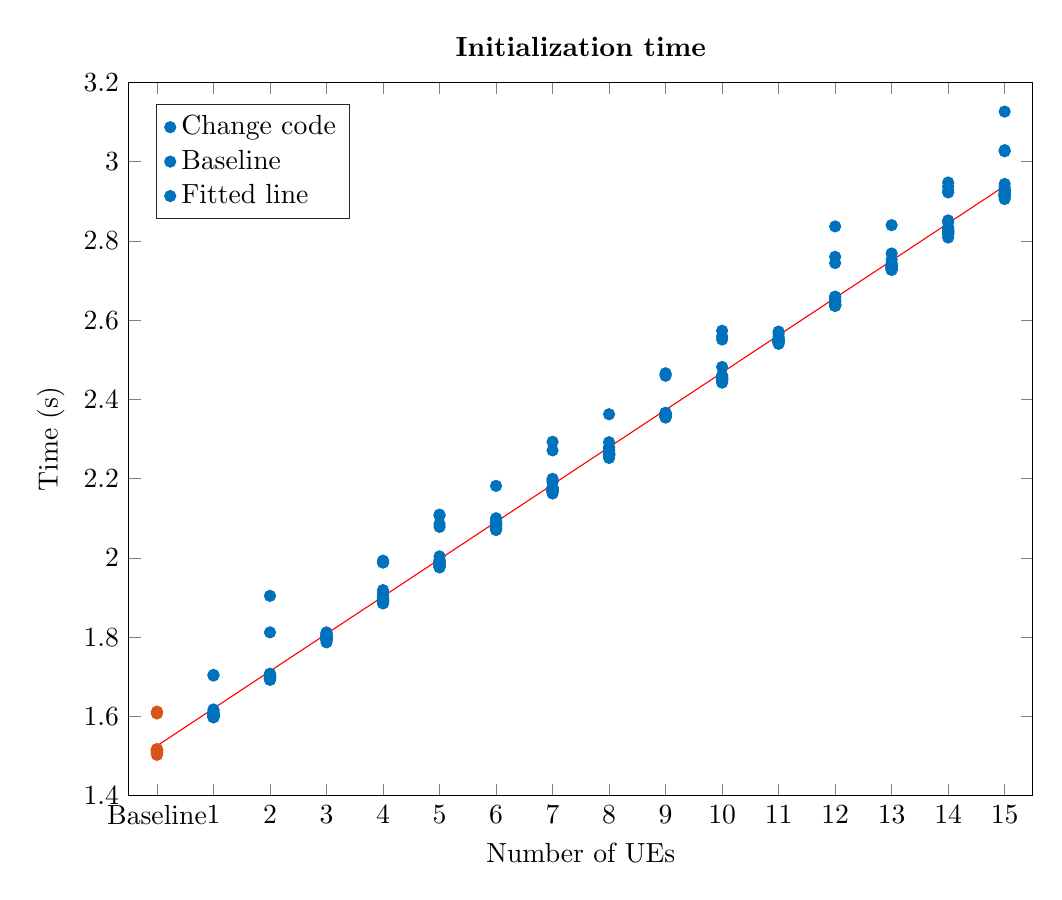
\begin{tikzpicture}

\begin{axis}[%
width=4.521in,
height=3.566in,
at={(0.758in,0.481in)},
scale only axis,
xmin=-0.5,
xmax=15.5,
xtick={0,1,2,3,4,5,6,7,8,9,10,11,12,13,14,15},
xticklabels={{Baseline},{1},{2},{3},{4},{5},{6},{7},{8},{9},{10},{11},{12},{13},{14},{15}},
xlabel={Number of UEs},
ymin=1.4,
ymax=3.2,
ylabel={Time (s)},
axis background/.style={fill=white},
title style={font=\bfseries},
title={Initialization time},
legend style={at={(0.03,0.97)},anchor=north west,legend cell align=left,align=left,draw=white!15!black}
]
\addplot [color=mycolor1,only marks,mark=*,mark options={solid}]
  table[row sep=crcr]{%
1	1.60657000541687\\
1	1.60206508636475\\
1	1.60402417182922\\
1	1.60998201370239\\
1	1.59828901290894\\
1	1.59890818595886\\
1	1.60678696632385\\
1	1.70481204986572\\
1	1.60345387458801\\
1	1.59799599647522\\
1	1.60137987136841\\
1	1.60408782958984\\
1	1.60380721092224\\
1	1.61764979362488\\
1	1.61315512657166\\
1	1.60408186912537\\
1	1.60214781761169\\
1	1.59820103645325\\
1	1.70323586463928\\
1	1.60239100456238\\
};
\addlegendentry{Change code};

\addplot [color=mycolor1,only marks,mark=*,mark options={solid}]
  table[row sep=crcr]{%
2	1.70376014709473\\
2	1.69752597808838\\
2	1.69991588592529\\
2	1.70224094390869\\
2	1.70335793495178\\
2	1.70019602775574\\
2	1.81223583221436\\
2	1.70259284973145\\
2	1.70058512687683\\
2	1.90431618690491\\
2	1.69746613502502\\
2	1.70056891441345\\
2	1.7057900428772\\
2	1.6926589012146\\
2	1.69660997390747\\
2	1.69284415245056\\
2	1.70735216140747\\
2	1.69585204124451\\
2	1.69405889511108\\
2	1.70744895935059\\
};
\addlegendentry{Baseline};

\addplot [color=mycolor1,only marks,mark=*,mark options={solid}]
  table[row sep=crcr]{%
3	1.79403805732727\\
3	1.80174088478088\\
3	1.80632400512695\\
3	1.79517197608948\\
3	1.7999119758606\\
3	1.80256199836731\\
3	1.79768395423889\\
3	1.79976677894592\\
3	1.79294800758362\\
3	1.80160784721375\\
3	1.81014108657837\\
3	1.8038489818573\\
3	1.79714298248291\\
3	1.78692388534546\\
3	1.80100011825562\\
3	1.79488515853882\\
3	1.81216788291931\\
3	1.79761385917664\\
3	1.80774402618408\\
3	1.79226994514465\\
};
\addlegendentry{Fitted line};

\addplot [color=mycolor1,only marks,mark=*,mark options={solid},forget plot]
  table[row sep=crcr]{%
4	1.98840284347534\\
4	1.98891401290894\\
4	1.90781497955322\\
4	1.90410208702087\\
4	1.89322519302368\\
4	1.89481401443481\\
4	1.89260292053223\\
4	1.89337205886841\\
4	1.89051008224487\\
4	1.99312591552734\\
4	1.89608120918274\\
4	1.98998594284058\\
4	1.9188380241394\\
4	1.88647603988647\\
4	1.89477205276489\\
4	1.89825892448425\\
4	1.90163683891296\\
4	1.89038610458374\\
4	1.91325998306274\\
4	1.88523697853088\\
};
\addplot [color=mycolor1,only marks,mark=*,mark options={solid},forget plot]
  table[row sep=crcr]{%
5	1.99140405654907\\
5	1.98323607444763\\
5	2.10928916931152\\
5	1.97859597206116\\
5	2.08593010902405\\
5	1.97863793373108\\
5	1.99062418937683\\
5	2.07845187187195\\
5	1.99165511131287\\
5	1.97789597511292\\
5	1.98802804946899\\
5	1.9954240322113\\
5	2.00401997566223\\
5	1.98706889152527\\
5	1.98496317863464\\
5	1.97689509391785\\
5	1.98235487937927\\
5	1.98183512687683\\
5	2.10645198822021\\
5	1.97618389129639\\
};
\addplot [color=mycolor1,only marks,mark=*,mark options={solid},forget plot]
  table[row sep=crcr]{%
6	2.07043600082397\\
6	2.08795213699341\\
6	2.08343291282654\\
6	2.09298491477966\\
6	2.07702803611755\\
6	2.07426118850708\\
6	2.1002459526062\\
6	2.09029412269592\\
6	2.08507609367371\\
6	2.07489895820618\\
6	2.08115887641907\\
6	2.09077501296997\\
6	2.08771395683289\\
6	2.07395005226135\\
6	2.07281303405762\\
6	2.1818699836731\\
6	2.08554911613464\\
6	2.0755889415741\\
6	2.09108996391296\\
6	2.08529710769653\\
};
\addplot [color=mycolor1,only marks,mark=*,mark options={solid},forget plot]
  table[row sep=crcr]{%
7	2.16757988929749\\
7	2.16262793540955\\
7	2.17564296722412\\
7	2.1759250164032\\
7	2.19155502319336\\
7	2.27151203155518\\
7	2.1676127910614\\
7	2.17567276954651\\
7	2.17186117172241\\
7	2.29317903518677\\
7	2.17238211631775\\
7	2.17540311813354\\
7	2.17659687995911\\
7	2.16815400123596\\
7	2.17439103126526\\
7	2.17733693122864\\
7	2.17026114463806\\
7	2.17389607429504\\
7	2.19961309432983\\
7	2.1946439743042\\
};
\addplot [color=mycolor1,only marks,mark=*,mark options={solid},forget plot]
  table[row sep=crcr]{%
8	2.27100706100464\\
8	2.26513481140137\\
8	2.26285195350647\\
8	2.2616548538208\\
8	2.27730703353882\\
8	2.27119493484497\\
8	2.26165103912354\\
8	2.25236415863037\\
8	2.26101899147034\\
8	2.36273288726807\\
8	2.25905799865723\\
8	2.27876305580139\\
8	2.29212021827698\\
8	2.26190590858459\\
8	2.27887606620789\\
8	2.25859999656677\\
8	2.26044893264771\\
8	2.26256895065308\\
8	2.26363897323608\\
8	2.26199913024902\\
};
\addplot [color=mycolor1,only marks,mark=*,mark options={solid},forget plot]
  table[row sep=crcr]{%
9	2.35985803604126\\
9	2.35758590698242\\
9	2.35490608215332\\
9	2.35805201530457\\
9	2.35813903808594\\
9	2.36619591712952\\
9	2.36291694641113\\
9	2.3615140914917\\
9	2.36494493484497\\
9	2.35645508766174\\
9	2.36352205276489\\
9	2.36592721939087\\
9	2.46607184410095\\
9	2.46248698234558\\
9	2.35874915122986\\
9	2.35979104042053\\
9	2.36403608322144\\
9	2.35437083244324\\
9	2.45976400375366\\
9	2.35649704933167\\
};
\addplot [color=mycolor1,only marks,mark=*,mark options={solid},forget plot]
  table[row sep=crcr]{%
10	2.4522500038147\\
10	2.45602107048035\\
10	2.45017790794373\\
10	2.46005892753601\\
10	2.4437301158905\\
10	2.45332884788513\\
10	2.45075607299805\\
10	2.44673299789429\\
10	2.44251298904419\\
10	2.45762705802917\\
10	2.45294904708862\\
10	2.48201680183411\\
10	2.45067620277405\\
10	2.57340097427368\\
10	2.44935178756714\\
10	2.45021200180054\\
10	2.55899405479431\\
10	2.55124402046204\\
10	2.45972394943237\\
10	2.4552149772644\\
};
\addplot [color=mycolor1,only marks,mark=*,mark options={solid},forget plot]
  table[row sep=crcr]{%
11	2.54409885406494\\
11	2.5580689907074\\
11	2.55131316184998\\
11	2.54538011550903\\
11	2.54991102218628\\
11	2.54586219787598\\
11	2.54519009590149\\
11	2.54685091972351\\
11	2.54958415031433\\
11	2.55115580558777\\
11	2.55340099334717\\
11	2.54899501800537\\
11	2.54859089851379\\
11	2.55042195320129\\
11	2.54939794540405\\
11	2.57132411003113\\
11	2.54307293891907\\
11	2.54036903381348\\
11	2.54952502250671\\
11	2.56598615646362\\
};
\addplot [color=mycolor1,only marks,mark=*,mark options={solid},forget plot]
  table[row sep=crcr]{%
12	2.63736891746521\\
12	2.6386501789093\\
12	2.63579487800598\\
12	2.76004385948181\\
12	2.64884686470032\\
12	2.63978505134583\\
12	2.65288496017456\\
12	2.6491858959198\\
12	2.64470791816711\\
12	2.65107917785645\\
12	2.83676886558533\\
12	2.63889098167419\\
12	2.65938687324524\\
12	2.6382257938385\\
12	2.63785290718079\\
12	2.65852999687195\\
12	2.74441695213318\\
12	2.64707398414612\\
12	2.63858604431152\\
12	2.65901207923889\\
};
\addplot [color=mycolor1,only marks,mark=*,mark options={solid},forget plot]
  table[row sep=crcr]{%
13	2.73925495147705\\
13	2.76844787597656\\
13	2.74468803405762\\
13	2.72794198989868\\
13	2.73288083076477\\
13	2.72759079933167\\
13	2.73981499671936\\
13	2.73808693885803\\
13	2.73037505149841\\
13	2.73060989379883\\
13	2.75299692153931\\
13	2.73150610923767\\
13	2.73392391204834\\
13	2.83988189697266\\
13	2.73668503761292\\
13	2.73319101333618\\
13	2.7269880771637\\
13	2.73366594314575\\
13	2.73546814918518\\
13	2.73145604133606\\
};
\addplot [color=mycolor1,only marks,mark=*,mark options={solid},forget plot]
  table[row sep=crcr]{%
14	2.93708896636963\\
14	2.8230938911438\\
14	2.82491183280945\\
14	2.81724190711975\\
14	2.83096098899841\\
14	2.82523608207703\\
14	2.92713284492493\\
14	2.83528399467468\\
14	2.81740093231201\\
14	2.94761514663696\\
14	2.84746098518372\\
14	2.92244791984558\\
14	2.82092189788818\\
14	2.82772517204285\\
14	2.82116103172302\\
14	2.8086531162262\\
14	2.82523202896118\\
14	2.82433700561523\\
14	2.85196495056152\\
14	2.82061409950256\\
};
\addplot [color=mycolor1,only marks,mark=*,mark options={solid},forget plot]
  table[row sep=crcr]{%
15	2.91355895996094\\
15	2.92956900596619\\
15	2.92799687385559\\
15	3.0291600227356\\
15	2.92018890380859\\
15	2.92904806137085\\
15	2.91579508781433\\
15	2.91569089889526\\
15	2.92359805107117\\
15	2.91793894767761\\
15	2.9355640411377\\
15	3.12653303146362\\
15	2.91362810134888\\
15	2.94397902488709\\
15	2.9135410785675\\
15	2.91744613647461\\
15	2.92062401771545\\
15	2.91158103942871\\
15	3.02637410163879\\
15	2.90584707260132\\
};
\addplot [color=mycolor2,only marks,mark=*,mark options={solid},forget plot]
  table[row sep=crcr]{%
0	1.51574110984802\\
0	1.60954785346985\\
0	1.61224007606506\\
0	1.51666712760925\\
0	1.51392078399658\\
0	1.51035499572754\\
0	1.50713300704956\\
0	1.51292109489441\\
0	1.51016092300415\\
0	1.5099790096283\\
0	1.51415991783142\\
0	1.51640319824219\\
0	1.51323890686035\\
0	1.51066589355469\\
0	1.5165901184082\\
0	1.50853300094604\\
0	1.50311899185181\\
0	1.60737919807434\\
0	1.51729917526245\\
0	1.50886988639832\\
};
\addplot [color=red,solid,forget plot]
  table[row sep=crcr]{%
0	1.52591009015129\\
0.015	1.52732309482467\\
0.03	1.52873609949805\\
0.045	1.53014910417142\\
0.06	1.5315621088448\\
0.075	1.53297511351818\\
0.09	1.53438811819156\\
0.105	1.53580112286494\\
0.12	1.53721412753832\\
0.135	1.5386271322117\\
0.15	1.54004013688508\\
0.165	1.54145314155845\\
0.18	1.54286614623183\\
0.195	1.54427915090521\\
0.21	1.54569215557859\\
0.225	1.54710516025197\\
0.24	1.54851816492535\\
0.255	1.54993116959873\\
0.27	1.55134417427211\\
0.285	1.55275717894549\\
0.3	1.55417018361886\\
0.315	1.55558318829224\\
0.33	1.55699619296562\\
0.345	1.558409197639\\
0.36	1.55982220231238\\
0.375	1.56123520698576\\
0.39	1.56264821165914\\
0.405	1.56406121633252\\
0.42	1.56547422100589\\
0.435	1.56688722567927\\
0.45	1.56830023035265\\
0.465	1.56971323502603\\
0.48	1.57112623969941\\
0.495	1.57253924437279\\
0.51	1.57395224904617\\
0.525	1.57536525371955\\
0.54	1.57677825839293\\
0.555	1.5781912630663\\
0.57	1.57960426773968\\
0.585	1.58101727241306\\
0.6	1.58243027708644\\
0.615	1.58384328175982\\
0.63	1.5852562864332\\
0.645	1.58666929110658\\
0.66	1.58808229577996\\
0.675	1.58949530045333\\
0.69	1.59090830512671\\
0.705	1.59232130980009\\
0.72	1.59373431447347\\
0.735	1.59514731914685\\
0.75	1.59656032382023\\
0.765	1.59797332849361\\
0.78	1.59938633316699\\
0.795	1.60079933784036\\
0.81	1.60221234251374\\
0.825	1.60362534718712\\
0.84	1.6050383518605\\
0.855	1.60645135653388\\
0.87	1.60786436120726\\
0.885	1.60927736588064\\
0.9	1.61069037055402\\
0.915	1.6121033752274\\
0.93	1.61351637990077\\
0.945	1.61492938457415\\
0.96	1.61634238924753\\
0.975	1.61775539392091\\
0.99	1.61916839859429\\
1.005	1.62058140326767\\
1.02	1.62199440794105\\
1.035	1.62340741261443\\
1.05	1.6248204172878\\
1.065	1.62623342196118\\
1.08	1.62764642663456\\
1.095	1.62905943130794\\
1.11	1.63047243598132\\
1.125	1.6318854406547\\
1.14	1.63329844532808\\
1.155	1.63471145000146\\
1.17	1.63612445467484\\
1.185	1.63753745934821\\
1.2	1.63895046402159\\
1.215	1.64036346869497\\
1.23	1.64177647336835\\
1.245	1.64318947804173\\
1.26	1.64460248271511\\
1.275	1.64601548738849\\
1.29	1.64742849206187\\
1.305	1.64884149673524\\
1.32	1.65025450140862\\
1.335	1.651667506082\\
1.35	1.65308051075538\\
1.365	1.65449351542876\\
1.38	1.65590652010214\\
1.395	1.65731952477552\\
1.41	1.6587325294489\\
1.425	1.66014553412227\\
1.44	1.66155853879565\\
1.455	1.66297154346903\\
1.47	1.66438454814241\\
1.485	1.66579755281579\\
1.5	1.66721055748917\\
1.515	1.66862356216255\\
1.53	1.67003656683593\\
1.545	1.67144957150931\\
1.56	1.67286257618268\\
1.575	1.67427558085606\\
1.59	1.67568858552944\\
1.605	1.67710159020282\\
1.62	1.6785145948762\\
1.635	1.67992759954958\\
1.65	1.68134060422296\\
1.665	1.68275360889634\\
1.68	1.68416661356971\\
1.695	1.68557961824309\\
1.71	1.68699262291647\\
1.725	1.68840562758985\\
1.74	1.68981863226323\\
1.755	1.69123163693661\\
1.77	1.69264464160999\\
1.785	1.69405764628337\\
1.8	1.69547065095674\\
1.815	1.69688365563012\\
1.83	1.6982966603035\\
1.845	1.69970966497688\\
1.86	1.70112266965026\\
1.875	1.70253567432364\\
1.89	1.70394867899702\\
1.905	1.7053616836704\\
1.92	1.70677468834378\\
1.935	1.70818769301715\\
1.95	1.70960069769053\\
1.965	1.71101370236391\\
1.98	1.71242670703729\\
1.995	1.71383971171067\\
2.01	1.71525271638405\\
2.025	1.71666572105743\\
2.04	1.71807872573081\\
2.055	1.71949173040418\\
2.07	1.72090473507756\\
2.085	1.72231773975094\\
2.1	1.72373074442432\\
2.115	1.7251437490977\\
2.13	1.72655675377108\\
2.145	1.72796975844446\\
2.16	1.72938276311784\\
2.175	1.73079576779121\\
2.19	1.73220877246459\\
2.205	1.73362177713797\\
2.22	1.73503478181135\\
2.235	1.73644778648473\\
2.25	1.73786079115811\\
2.265	1.73927379583149\\
2.28	1.74068680050487\\
2.295	1.74209980517825\\
2.31	1.74351280985162\\
2.325	1.744925814525\\
2.34	1.74633881919838\\
2.355	1.74775182387176\\
2.37	1.74916482854514\\
2.385	1.75057783321852\\
2.4	1.7519908378919\\
2.415	1.75340384256528\\
2.43	1.75481684723865\\
2.445	1.75622985191203\\
2.46	1.75764285658541\\
2.475	1.75905586125879\\
2.49	1.76046886593217\\
2.505	1.76188187060555\\
2.52	1.76329487527893\\
2.535	1.76470787995231\\
2.55	1.76612088462569\\
2.565	1.76753388929906\\
2.58	1.76894689397244\\
2.595	1.77035989864582\\
2.61	1.7717729033192\\
2.625	1.77318590799258\\
2.64	1.77459891266596\\
2.655	1.77601191733934\\
2.67	1.77742492201272\\
2.685	1.77883792668609\\
2.7	1.78025093135947\\
2.715	1.78166393603285\\
2.73	1.78307694070623\\
2.745	1.78448994537961\\
2.76	1.78590295005299\\
2.775	1.78731595472637\\
2.79	1.78872895939975\\
2.805	1.79014196407312\\
2.82	1.7915549687465\\
2.835	1.79296797341988\\
2.85	1.79438097809326\\
2.865	1.79579398276664\\
2.88	1.79720698744002\\
2.895	1.7986199921134\\
2.91	1.80003299678678\\
2.925	1.80144600146016\\
2.94	1.80285900613353\\
2.955	1.80427201080691\\
2.97	1.80568501548029\\
2.985	1.80709802015367\\
3	1.80851102482705\\
3.015	1.80992402950043\\
3.03	1.81133703417381\\
3.045	1.81275003884719\\
3.06	1.81416304352056\\
3.075	1.81557604819394\\
3.09	1.81698905286732\\
3.105	1.8184020575407\\
3.12	1.81981506221408\\
3.135	1.82122806688746\\
3.15	1.82264107156084\\
3.165	1.82405407623422\\
3.18	1.8254670809076\\
3.195	1.82688008558097\\
3.21	1.82829309025435\\
3.225	1.82970609492773\\
3.24	1.83111909960111\\
3.255	1.83253210427449\\
3.27	1.83394510894787\\
3.285	1.83535811362125\\
3.3	1.83677111829463\\
3.315	1.838184122968\\
3.33	1.83959712764138\\
3.345	1.84101013231476\\
3.36	1.84242313698814\\
3.375	1.84383614166152\\
3.39	1.8452491463349\\
3.405	1.84666215100828\\
3.42	1.84807515568166\\
3.435	1.84948816035503\\
3.45	1.85090116502841\\
3.465	1.85231416970179\\
3.48	1.85372717437517\\
3.495	1.85514017904855\\
3.51	1.85655318372193\\
3.525	1.85796618839531\\
3.54	1.85937919306869\\
3.555	1.86079219774207\\
3.57	1.86220520241544\\
3.585	1.86361820708882\\
3.6	1.8650312117622\\
3.615	1.86644421643558\\
3.63	1.86785722110896\\
3.645	1.86927022578234\\
3.66	1.87068323045572\\
3.675	1.8720962351291\\
3.69	1.87350923980247\\
3.705	1.87492224447585\\
3.72	1.87633524914923\\
3.735	1.87774825382261\\
3.75	1.87916125849599\\
3.765	1.88057426316937\\
3.78	1.88198726784275\\
3.795	1.88340027251613\\
3.81	1.88481327718951\\
3.825	1.88622628186288\\
3.84	1.88763928653626\\
3.855	1.88905229120964\\
3.87	1.89046529588302\\
3.885	1.8918783005564\\
3.9	1.89329130522978\\
3.915	1.89470430990316\\
3.93	1.89611731457654\\
3.945	1.89753031924991\\
3.96	1.89894332392329\\
3.975	1.90035632859667\\
3.99	1.90176933327005\\
4.005	1.90318233794343\\
4.02	1.90459534261681\\
4.035	1.90600834729019\\
4.05	1.90742135196357\\
4.065	1.90883435663694\\
4.08	1.91024736131032\\
4.095	1.9116603659837\\
4.11	1.91307337065708\\
4.125	1.91448637533046\\
4.14	1.91589938000384\\
4.155	1.91731238467722\\
4.17	1.9187253893506\\
4.185	1.92013839402397\\
4.2	1.92155139869735\\
4.215	1.92296440337073\\
4.23	1.92437740804411\\
4.245	1.92579041271749\\
4.26	1.92720341739087\\
4.275	1.92861642206425\\
4.29	1.93002942673763\\
4.305	1.93144243141101\\
4.32	1.93285543608438\\
4.335	1.93426844075776\\
4.35	1.93568144543114\\
4.365	1.93709445010452\\
4.38	1.9385074547779\\
4.395	1.93992045945128\\
4.41	1.94133346412466\\
4.425	1.94274646879804\\
4.44	1.94415947347141\\
4.455	1.94557247814479\\
4.47	1.94698548281817\\
4.485	1.94839848749155\\
4.5	1.94981149216493\\
4.515	1.95122449683831\\
4.53	1.95263750151169\\
4.545	1.95405050618507\\
4.56	1.95546351085845\\
4.575	1.95687651553182\\
4.59	1.9582895202052\\
4.605	1.95970252487858\\
4.62	1.96111552955196\\
4.635	1.96252853422534\\
4.65	1.96394153889872\\
4.665	1.9653545435721\\
4.68	1.96676754824548\\
4.695	1.96818055291885\\
4.71	1.96959355759223\\
4.725	1.97100656226561\\
4.74	1.97241956693899\\
4.755	1.97383257161237\\
4.77	1.97524557628575\\
4.785	1.97665858095913\\
4.8	1.97807158563251\\
4.815	1.97948459030588\\
4.83	1.98089759497926\\
4.845	1.98231059965264\\
4.86	1.98372360432602\\
4.875	1.9851366089994\\
4.89	1.98654961367278\\
4.905	1.98796261834616\\
4.92	1.98937562301954\\
4.935	1.99078862769292\\
4.95	1.99220163236629\\
4.965	1.99361463703967\\
4.98	1.99502764171305\\
4.995	1.99644064638643\\
5.01	1.99785365105981\\
5.025	1.99926665573319\\
5.04	2.00067966040657\\
5.055	2.00209266507995\\
5.07	2.00350566975332\\
5.085	2.0049186744267\\
5.1	2.00633167910008\\
5.115	2.00774468377346\\
5.13	2.00915768844684\\
5.145	2.01057069312022\\
5.16	2.0119836977936\\
5.175	2.01339670246698\\
5.19	2.01480970714035\\
5.205	2.01622271181373\\
5.22	2.01763571648711\\
5.235	2.01904872116049\\
5.25	2.02046172583387\\
5.265	2.02187473050725\\
5.28	2.02328773518063\\
5.295	2.02470073985401\\
5.31	2.02611374452739\\
5.325	2.02752674920076\\
5.34	2.02893975387414\\
5.355	2.03035275854752\\
5.37	2.0317657632209\\
5.385	2.03317876789428\\
5.4	2.03459177256766\\
5.415	2.03600477724104\\
5.43	2.03741778191442\\
5.445	2.03883078658779\\
5.46	2.04024379126117\\
5.475	2.04165679593455\\
5.49	2.04306980060793\\
5.505	2.04448280528131\\
5.52	2.04589580995469\\
5.535	2.04730881462807\\
5.55	2.04872181930145\\
5.565	2.05013482397483\\
5.58	2.0515478286482\\
5.595	2.05296083332158\\
5.61	2.05437383799496\\
5.625	2.05578684266834\\
5.64	2.05719984734172\\
5.655	2.0586128520151\\
5.67	2.06002585668848\\
5.685	2.06143886136186\\
5.7	2.06285186603523\\
5.715	2.06426487070861\\
5.73	2.06567787538199\\
5.745	2.06709088005537\\
5.76	2.06850388472875\\
5.775	2.06991688940213\\
5.79	2.07132989407551\\
5.805	2.07274289874889\\
5.82	2.07415590342226\\
5.835	2.07556890809564\\
5.85	2.07698191276902\\
5.865	2.0783949174424\\
5.88	2.07980792211578\\
5.895	2.08122092678916\\
5.91	2.08263393146254\\
5.925	2.08404693613592\\
5.94	2.0854599408093\\
5.955	2.08687294548267\\
5.97	2.08828595015605\\
5.985	2.08969895482943\\
6	2.09111195950281\\
6.015	2.09252496417619\\
6.03	2.09393796884957\\
6.045	2.09535097352295\\
6.06	2.09676397819633\\
6.075	2.0981769828697\\
6.09	2.09958998754308\\
6.105	2.10100299221646\\
6.12	2.10241599688984\\
6.135	2.10382900156322\\
6.15	2.1052420062366\\
6.165	2.10665501090998\\
6.18	2.10806801558336\\
6.195	2.10948102025674\\
6.21	2.11089402493011\\
6.225	2.11230702960349\\
6.24	2.11372003427687\\
6.255	2.11513303895025\\
6.27	2.11654604362363\\
6.285	2.11795904829701\\
6.3	2.11937205297039\\
6.315	2.12078505764377\\
6.33	2.12219806231714\\
6.345	2.12361106699052\\
6.36	2.1250240716639\\
6.375	2.12643707633728\\
6.39	2.12785008101066\\
6.405	2.12926308568404\\
6.42	2.13067609035742\\
6.435	2.1320890950308\\
6.45	2.13350209970417\\
6.465	2.13491510437755\\
6.48	2.13632810905093\\
6.495	2.13774111372431\\
6.51	2.13915411839769\\
6.525	2.14056712307107\\
6.54	2.14198012774445\\
6.555	2.14339313241783\\
6.57	2.14480613709121\\
6.585	2.14621914176458\\
6.6	2.14763214643796\\
6.615	2.14904515111134\\
6.63	2.15045815578472\\
6.645	2.1518711604581\\
6.66	2.15328416513148\\
6.675	2.15469716980486\\
6.69	2.15611017447824\\
6.705	2.15752317915161\\
6.72	2.15893618382499\\
6.735	2.16034918849837\\
6.75	2.16176219317175\\
6.765	2.16317519784513\\
6.78	2.16458820251851\\
6.795	2.16600120719189\\
6.81	2.16741421186527\\
6.825	2.16882721653865\\
6.84	2.17024022121202\\
6.855	2.1716532258854\\
6.87	2.17306623055878\\
6.885	2.17447923523216\\
6.9	2.17589223990554\\
6.915	2.17730524457892\\
6.93	2.1787182492523\\
6.945	2.18013125392568\\
6.96	2.18154425859905\\
6.975	2.18295726327243\\
6.99	2.18437026794581\\
7.005	2.18578327261919\\
7.02	2.18719627729257\\
7.035	2.18860928196595\\
7.05	2.19002228663933\\
7.065	2.19143529131271\\
7.08	2.19284829598608\\
7.095	2.19426130065946\\
7.11	2.19567430533284\\
7.125	2.19708731000622\\
7.14	2.1985003146796\\
7.155	2.19991331935298\\
7.17	2.20132632402636\\
7.185	2.20273932869974\\
7.2	2.20415233337312\\
7.215	2.20556533804649\\
7.23	2.20697834271987\\
7.245	2.20839134739325\\
7.26	2.20980435206663\\
7.275	2.21121735674001\\
7.29	2.21263036141339\\
7.305	2.21404336608677\\
7.32	2.21545637076015\\
7.335	2.21686937543352\\
7.35	2.2182823801069\\
7.365	2.21969538478028\\
7.38	2.22110838945366\\
7.395	2.22252139412704\\
7.41	2.22393439880042\\
7.425	2.2253474034738\\
7.44	2.22676040814718\\
7.455	2.22817341282055\\
7.47	2.22958641749393\\
7.485	2.23099942216731\\
7.5	2.23241242684069\\
7.515	2.23382543151407\\
7.53	2.23523843618745\\
7.545	2.23665144086083\\
7.56	2.23806444553421\\
7.575	2.23947745020759\\
7.59	2.24089045488096\\
7.605	2.24230345955434\\
7.62	2.24371646422772\\
7.635	2.2451294689011\\
7.65	2.24654247357448\\
7.665	2.24795547824786\\
7.68	2.24936848292124\\
7.695	2.25078148759462\\
7.71	2.25219449226799\\
7.725	2.25360749694137\\
7.74	2.25502050161475\\
7.755	2.25643350628813\\
7.77	2.25784651096151\\
7.785	2.25925951563489\\
7.8	2.26067252030827\\
7.815	2.26208552498165\\
7.83	2.26349852965503\\
7.845	2.2649115343284\\
7.86	2.26632453900178\\
7.875	2.26773754367516\\
7.89	2.26915054834854\\
7.905	2.27056355302192\\
7.92	2.2719765576953\\
7.935	2.27338956236868\\
7.95	2.27480256704206\\
7.965	2.27621557171543\\
7.98	2.27762857638881\\
7.995	2.27904158106219\\
8.01	2.28045458573557\\
8.025	2.28186759040895\\
8.04	2.28328059508233\\
8.055	2.28469359975571\\
8.07	2.28610660442909\\
8.085	2.28751960910246\\
8.1	2.28893261377584\\
8.115	2.29034561844922\\
8.13	2.2917586231226\\
8.145	2.29317162779598\\
8.16	2.29458463246936\\
8.175	2.29599763714274\\
8.19	2.29741064181612\\
8.205	2.2988236464895\\
8.22	2.30023665116287\\
8.235	2.30164965583625\\
8.25	2.30306266050963\\
8.265	2.30447566518301\\
8.28	2.30588866985639\\
8.295	2.30730167452977\\
8.31	2.30871467920315\\
8.325	2.31012768387653\\
8.34	2.3115406885499\\
8.355	2.31295369322328\\
8.37	2.31436669789666\\
8.385	2.31577970257004\\
8.4	2.31719270724342\\
8.415	2.3186057119168\\
8.43	2.32001871659018\\
8.445	2.32143172126356\\
8.46	2.32284472593693\\
8.475	2.32425773061031\\
8.49	2.32567073528369\\
8.505	2.32708373995707\\
8.52	2.32849674463045\\
8.535	2.32990974930383\\
8.55	2.33132275397721\\
8.565	2.33273575865059\\
8.58	2.33414876332397\\
8.595	2.33556176799734\\
8.61	2.33697477267072\\
8.625	2.3383877773441\\
8.64	2.33980078201748\\
8.655	2.34121378669086\\
8.67	2.34262679136424\\
8.685	2.34403979603762\\
8.7	2.345452800711\\
8.715	2.34686580538437\\
8.73	2.34827881005775\\
8.745	2.34969181473113\\
8.76	2.35110481940451\\
8.775	2.35251782407789\\
8.79	2.35393082875127\\
8.805	2.35534383342465\\
8.82	2.35675683809803\\
8.835	2.3581698427714\\
8.85	2.35958284744478\\
8.865	2.36099585211816\\
8.88	2.36240885679154\\
8.895	2.36382186146492\\
8.91	2.3652348661383\\
8.925	2.36664787081168\\
8.94	2.36806087548506\\
8.955	2.36947388015844\\
8.97	2.37088688483181\\
8.985	2.37229988950519\\
9	2.37371289417857\\
9.015	2.37512589885195\\
9.03	2.37653890352533\\
9.045	2.37795190819871\\
9.06	2.37936491287209\\
9.075	2.38077791754547\\
9.09	2.38219092221884\\
9.105	2.38360392689222\\
9.12	2.3850169315656\\
9.135	2.38642993623898\\
9.15	2.38784294091236\\
9.165	2.38925594558574\\
9.18	2.39066895025912\\
9.195	2.3920819549325\\
9.21	2.39349495960588\\
9.225	2.39490796427925\\
9.24	2.39632096895263\\
9.255	2.39773397362601\\
9.27	2.39914697829939\\
9.285	2.40055998297277\\
9.3	2.40197298764615\\
9.315	2.40338599231953\\
9.33	2.40479899699291\\
9.345	2.40621200166628\\
9.36	2.40762500633966\\
9.375	2.40903801101304\\
9.39	2.41045101568642\\
9.405	2.4118640203598\\
9.42	2.41327702503318\\
9.435	2.41469002970656\\
9.45	2.41610303437994\\
9.465	2.41751603905331\\
9.48	2.41892904372669\\
9.495	2.42034204840007\\
9.51	2.42175505307345\\
9.525	2.42316805774683\\
9.54	2.42458106242021\\
9.555	2.42599406709359\\
9.57	2.42740707176697\\
9.585	2.42882007644035\\
9.6	2.43023308111372\\
9.615	2.4316460857871\\
9.63	2.43305909046048\\
9.645	2.43447209513386\\
9.66	2.43588509980724\\
9.675	2.43729810448062\\
9.69	2.438711109154\\
9.705	2.44012411382738\\
9.72	2.44153711850075\\
9.735	2.44295012317413\\
9.75	2.44436312784751\\
9.765	2.44577613252089\\
9.78	2.44718913719427\\
9.795	2.44860214186765\\
9.81	2.45001514654103\\
9.825	2.45142815121441\\
9.84	2.45284115588779\\
9.855	2.45425416056116\\
9.87	2.45566716523454\\
9.885	2.45708016990792\\
9.9	2.4584931745813\\
9.915	2.45990617925468\\
9.93	2.46131918392806\\
9.945	2.46273218860144\\
9.96	2.46414519327482\\
9.975	2.46555819794819\\
9.99	2.46697120262157\\
10.005	2.46838420729495\\
10.02	2.46979721196833\\
10.035	2.47121021664171\\
10.05	2.47262322131509\\
10.065	2.47403622598847\\
10.08	2.47544923066185\\
10.095	2.47686223533522\\
10.11	2.4782752400086\\
10.125	2.47968824468198\\
10.14	2.48110124935536\\
10.155	2.48251425402874\\
10.17	2.48392725870212\\
10.185	2.4853402633755\\
10.2	2.48675326804888\\
10.215	2.48816627272226\\
10.23	2.48957927739563\\
10.245	2.49099228206901\\
10.26	2.49240528674239\\
10.275	2.49381829141577\\
10.29	2.49523129608915\\
10.305	2.49664430076253\\
10.32	2.49805730543591\\
10.335	2.49947031010929\\
10.35	2.50088331478266\\
10.365	2.50229631945604\\
10.38	2.50370932412942\\
10.395	2.5051223288028\\
10.41	2.50653533347618\\
10.425	2.50794833814956\\
10.44	2.50936134282294\\
10.455	2.51077434749632\\
10.47	2.51218735216969\\
10.485	2.51360035684307\\
10.5	2.51501336151645\\
10.515	2.51642636618983\\
10.53	2.51783937086321\\
10.545	2.51925237553659\\
10.56	2.52066538020997\\
10.575	2.52207838488335\\
10.59	2.52349138955673\\
10.605	2.5249043942301\\
10.62	2.52631739890348\\
10.635	2.52773040357686\\
10.65	2.52914340825024\\
10.665	2.53055641292362\\
10.68	2.531969417597\\
10.695	2.53338242227038\\
10.71	2.53479542694376\\
10.725	2.53620843161713\\
10.74	2.53762143629051\\
10.755	2.53903444096389\\
10.77	2.54044744563727\\
10.785	2.54186045031065\\
10.8	2.54327345498403\\
10.815	2.54468645965741\\
10.83	2.54609946433079\\
10.845	2.54751246900417\\
10.86	2.54892547367754\\
10.875	2.55033847835092\\
10.89	2.5517514830243\\
10.905	2.55316448769768\\
10.92	2.55457749237106\\
10.935	2.55599049704444\\
10.95	2.55740350171782\\
10.965	2.5588165063912\\
10.98	2.56022951106457\\
10.995	2.56164251573795\\
11.01	2.56305552041133\\
11.025	2.56446852508471\\
11.04	2.56588152975809\\
11.055	2.56729453443147\\
11.07	2.56870753910485\\
11.085	2.57012054377823\\
11.1	2.5715335484516\\
11.115	2.57294655312498\\
11.13	2.57435955779836\\
11.145	2.57577256247174\\
11.16	2.57718556714512\\
11.175	2.5785985718185\\
11.19	2.58001157649188\\
11.205	2.58142458116526\\
11.22	2.58283758583864\\
11.235	2.58425059051201\\
11.25	2.58566359518539\\
11.265	2.58707659985877\\
11.28	2.58848960453215\\
11.295	2.58990260920553\\
11.31	2.59131561387891\\
11.325	2.59272861855229\\
11.34	2.59414162322567\\
11.355	2.59555462789904\\
11.37	2.59696763257242\\
11.385	2.5983806372458\\
11.4	2.59979364191918\\
11.415	2.60120664659256\\
11.43	2.60261965126594\\
11.445	2.60403265593932\\
11.46	2.6054456606127\\
11.475	2.60685866528608\\
11.49	2.60827166995945\\
11.505	2.60968467463283\\
11.52	2.61109767930621\\
11.535	2.61251068397959\\
11.55	2.61392368865297\\
11.565	2.61533669332635\\
11.58	2.61674969799973\\
11.595	2.61816270267311\\
11.61	2.61957570734648\\
11.625	2.62098871201986\\
11.64	2.62240171669324\\
11.655	2.62381472136662\\
11.67	2.62522772604\\
11.685	2.62664073071338\\
11.7	2.62805373538676\\
11.715	2.62946674006014\\
11.73	2.63087974473351\\
11.745	2.63229274940689\\
11.76	2.63370575408027\\
11.775	2.63511875875365\\
11.79	2.63653176342703\\
11.805	2.63794476810041\\
11.82	2.63935777277379\\
11.835	2.64077077744717\\
11.85	2.64218378212054\\
11.865	2.64359678679392\\
11.88	2.6450097914673\\
11.895	2.64642279614068\\
11.91	2.64783580081406\\
11.925	2.64924880548744\\
11.94	2.65066181016082\\
11.955	2.6520748148342\\
11.97	2.65348781950758\\
11.985	2.65490082418095\\
12	2.65631382885433\\
12.015	2.65772683352771\\
12.03	2.65913983820109\\
12.045	2.66055284287447\\
12.06	2.66196584754785\\
12.075	2.66337885222123\\
12.09	2.66479185689461\\
12.105	2.66620486156798\\
12.12	2.66761786624136\\
12.135	2.66903087091474\\
12.15	2.67044387558812\\
12.165	2.6718568802615\\
12.18	2.67326988493488\\
12.195	2.67468288960826\\
12.21	2.67609589428164\\
12.225	2.67750889895502\\
12.24	2.67892190362839\\
12.255	2.68033490830177\\
12.27	2.68174791297515\\
12.285	2.68316091764853\\
12.3	2.68457392232191\\
12.315	2.68598692699529\\
12.33	2.68739993166867\\
12.345	2.68881293634205\\
12.36	2.69022594101542\\
12.375	2.6916389456888\\
12.39	2.69305195036218\\
12.405	2.69446495503556\\
12.42	2.69587795970894\\
12.435	2.69729096438232\\
12.45	2.6987039690557\\
12.465	2.70011697372908\\
12.48	2.70152997840245\\
12.495	2.70294298307583\\
12.51	2.70435598774921\\
12.525	2.70576899242259\\
12.54	2.70718199709597\\
12.555	2.70859500176935\\
12.57	2.71000800644273\\
12.585	2.71142101111611\\
12.6	2.71283401578949\\
12.615	2.71424702046286\\
12.63	2.71566002513624\\
12.645	2.71707302980962\\
12.66	2.718486034483\\
12.675	2.71989903915638\\
12.69	2.72131204382976\\
12.705	2.72272504850314\\
12.72	2.72413805317652\\
12.735	2.72555105784989\\
12.75	2.72696406252327\\
12.765	2.72837706719665\\
12.78	2.72979007187003\\
12.795	2.73120307654341\\
12.81	2.73261608121679\\
12.825	2.73402908589017\\
12.84	2.73544209056355\\
12.855	2.73685509523693\\
12.87	2.7382680999103\\
12.885	2.73968110458368\\
12.9	2.74109410925706\\
12.915	2.74250711393044\\
12.93	2.74392011860382\\
12.945	2.7453331232772\\
12.96	2.74674612795058\\
12.975	2.74815913262396\\
12.99	2.74957213729733\\
13.005	2.75098514197071\\
13.02	2.75239814664409\\
13.035	2.75381115131747\\
13.05	2.75522415599085\\
13.065	2.75663716066423\\
13.08	2.75805016533761\\
13.095	2.75946317001099\\
13.11	2.76087617468436\\
13.125	2.76228917935774\\
13.14	2.76370218403112\\
13.155	2.7651151887045\\
13.17	2.76652819337788\\
13.185	2.76794119805126\\
13.2	2.76935420272464\\
13.215	2.77076720739802\\
13.23	2.7721802120714\\
13.245	2.77359321674477\\
13.26	2.77500622141815\\
13.275	2.77641922609153\\
13.29	2.77783223076491\\
13.305	2.77924523543829\\
13.32	2.78065824011167\\
13.335	2.78207124478505\\
13.35	2.78348424945843\\
13.365	2.7848972541318\\
13.38	2.78631025880518\\
13.395	2.78772326347856\\
13.41	2.78913626815194\\
13.425	2.79054927282532\\
13.44	2.7919622774987\\
13.455	2.79337528217208\\
13.47	2.79478828684546\\
13.485	2.79620129151883\\
13.5	2.79761429619221\\
13.515	2.79902730086559\\
13.53	2.80044030553897\\
13.545	2.80185331021235\\
13.56	2.80326631488573\\
13.575	2.80467931955911\\
13.59	2.80609232423249\\
13.605	2.80750532890587\\
13.62	2.80891833357924\\
13.635	2.81033133825262\\
13.65	2.811744342926\\
13.665	2.81315734759938\\
13.68	2.81457035227276\\
13.695	2.81598335694614\\
13.71	2.81739636161952\\
13.725	2.8188093662929\\
13.74	2.82022237096627\\
13.755	2.82163537563965\\
13.77	2.82304838031303\\
13.785	2.82446138498641\\
13.8	2.82587438965979\\
13.815	2.82728739433317\\
13.83	2.82870039900655\\
13.845	2.83011340367993\\
13.86	2.83152640835331\\
13.875	2.83293941302668\\
13.89	2.83435241770006\\
13.905	2.83576542237344\\
13.92	2.83717842704682\\
13.935	2.8385914317202\\
13.95	2.84000443639358\\
13.965	2.84141744106696\\
13.98	2.84283044574034\\
13.995	2.84424345041371\\
14.01	2.84565645508709\\
14.025	2.84706945976047\\
14.04	2.84848246443385\\
14.055	2.84989546910723\\
14.07	2.85130847378061\\
14.085	2.85272147845399\\
14.1	2.85413448312737\\
14.115	2.85554748780075\\
14.13	2.85696049247412\\
14.145	2.8583734971475\\
14.16	2.85978650182088\\
14.175	2.86119950649426\\
14.19	2.86261251116764\\
14.205	2.86402551584102\\
14.22	2.8654385205144\\
14.235	2.86685152518778\\
14.25	2.86826452986115\\
14.265	2.86967753453453\\
14.28	2.87109053920791\\
14.295	2.87250354388129\\
14.31	2.87391654855467\\
14.325	2.87532955322805\\
14.34	2.87674255790143\\
14.355	2.87815556257481\\
14.37	2.87956856724818\\
14.385	2.88098157192156\\
14.4	2.88239457659494\\
14.415	2.88380758126832\\
14.43	2.8852205859417\\
14.445	2.88663359061508\\
14.46	2.88804659528846\\
14.475	2.88945959996184\\
14.49	2.89087260463522\\
14.505	2.89228560930859\\
14.52	2.89369861398197\\
14.535	2.89511161865535\\
14.55	2.89652462332873\\
14.565	2.89793762800211\\
14.58	2.89935063267549\\
14.595	2.90076363734887\\
14.61	2.90217664202225\\
14.625	2.90358964669562\\
14.64	2.905002651369\\
14.655	2.90641565604238\\
14.67	2.90782866071576\\
14.685	2.90924166538914\\
14.7	2.91065467006252\\
14.715	2.9120676747359\\
14.73	2.91348067940928\\
14.745	2.91489368408265\\
14.76	2.91630668875603\\
14.775	2.91771969342941\\
14.79	2.91913269810279\\
14.805	2.92054570277617\\
14.82	2.92195870744955\\
14.835	2.92337171212293\\
14.85	2.92478471679631\\
14.865	2.92619772146969\\
14.88	2.92761072614306\\
14.895	2.92902373081644\\
14.91	2.93043673548982\\
14.925	2.9318497401632\\
14.94	2.93326274483658\\
14.955	2.93467574950996\\
14.97	2.93608875418334\\
14.985	2.93750175885672\\
15	2.93891476353009\\
};
\end{axis}
\end{tikzpicture}%
\caption{Execution time for the initialization, for different number of devices and the baseline emulator. The fitted line is a linear approximation.}
\label{fig:MT_Init_Time}
\end{figure}

From \autoref{fig:MT_Init_Time} it can be seen that there is a linear tendency scaling with the number of devices. It is also seen that even if the baseline emulator and the MDE emulates one device, the baseline emulator have a lower execution time, with a estimated difference to be the same as a single step between different number of devices. The fitted line is estimated to be:

\begin{align}
&T_{init} (\text{NoD}) = 0.0942 \cdot \text{NoD} + 1.526 
\end{align}
\begin{where}
\va{$T_{Init}$}{is the execution time for the initialization step}{s}
\va{$\text{NoD}$}{is the number of devices emulated}{$\cdot$}
\end{where}


\subsection{Synchronization}
The execution time for the synchronization step is measured from the start of cell search to the start of the MIB-NB decoding, which gives the results seen on \autoref{fig:MT_Sync_Time}. As the error type cell sync, mentioned in \autoref{sec:MTerror}, occurs in this step of the process, some measurements will be equal to zero, as the execution time can not be calculated, due to fact that the measurement ends when an error occur. This impacts the number of measurement points further on as well.

\captionsetup{belowskip=0em}
\begin{minipage}{0.48\textwidth}
\begin{figure}[H]
\tikzsetnextfilename{MT_Sync_Time}
\centering
\resizebox{\textwidth}{!}{
% This file was created by matlab2tikz.
%
%The latest updates can be retrieved from
%  http://www.mathworks.com/matlabcentral/fileexchange/22022-matlab2tikz-matlab2tikz
%where you can also make suggestions and rate matlab2tikz.
%
\definecolor{mycolor1}{rgb}{0.00000,0.44700,0.74100}%
\definecolor{mycolor2}{rgb}{0.85000,0.32500,0.09800}%
%
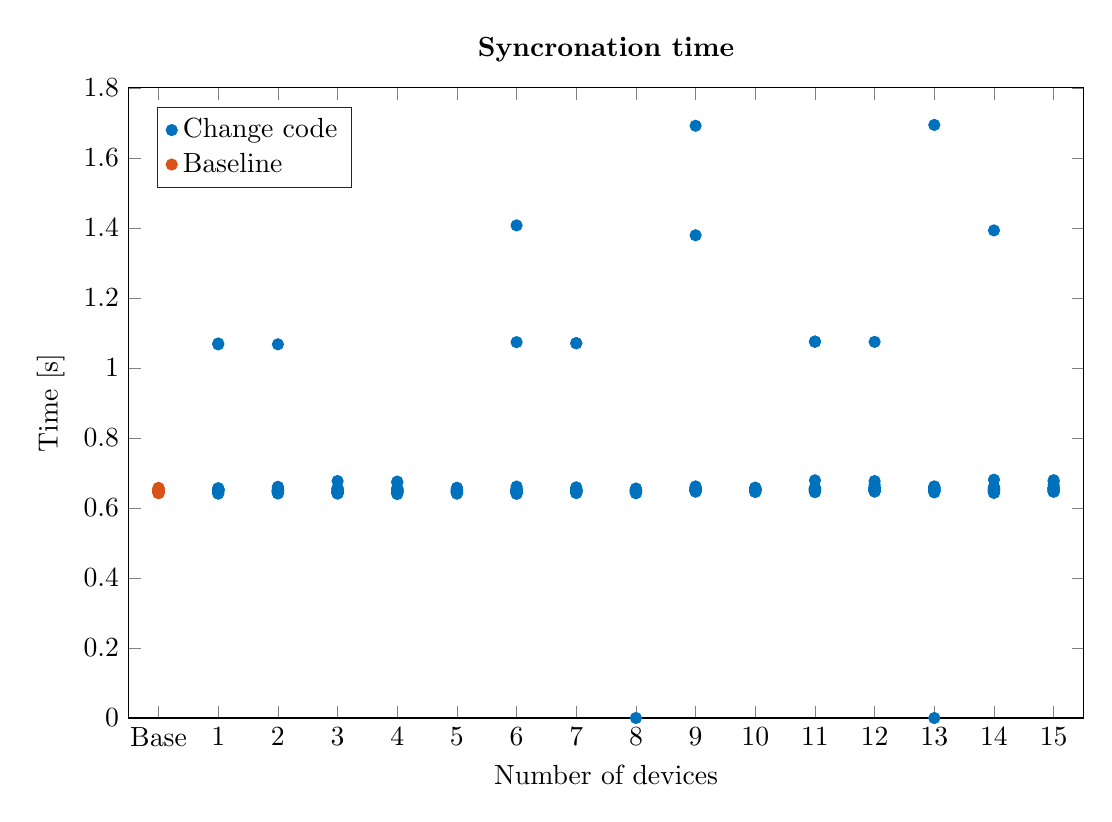
\begin{tikzpicture}

\begin{axis}[%
width=\textwidth,
height=.66\textwidth,
at={(0.758in,0.481in)},
scale only axis,
xmin=-0.5,
xmax=15.5,
xtick={0,1,2,3,4,5,6,7,8,9,10,11,12,13,14,15},
xticklabels={{Base},{1},{2},{3},{4},{5},{6},{7},{8},{9},{10},{11},{12},{13},{14},{15}},
xlabel={Number of devices},
ymin=0,
ymax=1.8,
ylabel={Time [s]},
axis background/.style={fill=white},
title style={font=\bfseries},
title={Syncronation time},
legend style={at={(0.03,0.97)},anchor=north west,legend cell align=left,align=left,draw=white!15!black}
]
\addplot [color=mycolor1,only marks,mark=*,mark options={solid}]
  table[row sep=crcr]{%
1	0.650609970092773\\
1	0.653857946395874\\
1	0.640816926956177\\
1	0.642185926437378\\
1	0.645545959472656\\
1	1.06731581687927\\
1	0.649732112884521\\
1	0.653727054595947\\
1	1.06988906860352\\
1	0.648482799530029\\
1	0.650296926498413\\
1	0.653731107711792\\
1	0.650707960128784\\
1	0.656582117080688\\
1	0.651366949081421\\
1	0.653976202011108\\
1	0.653213024139404\\
1	0.650224924087524\\
1	0.648483037948608\\
1	0.654691934585571\\
};
\addlegendentry{Change code};

\addplot [color=mycolor1,only marks,mark=*,mark options={solid},forget plot]
  table[row sep=crcr]{%
2	0.646949052810669\\
2	0.649175882339478\\
2	0.650078058242798\\
2	0.658921957015991\\
2	0.644191026687622\\
2	1.06752800941467\\
2	0.652630090713501\\
2	0.649014949798584\\
2	0.650974988937378\\
2	0.660398006439209\\
2	0.641355037689209\\
2	0.652486085891724\\
2	0.646153926849365\\
2	0.645971059799194\\
2	0.647706985473633\\
2	0.652987003326416\\
2	0.651640892028809\\
2	0.64258599281311\\
2	0.644962072372437\\
2	0.649473905563354\\
};


\addplot [color=mycolor1,only marks,mark=*,mark options={solid},forget plot]
  table[row sep=crcr]{%
3	0.643748044967651\\
3	0.644491195678711\\
3	0.642645835876465\\
3	0.656013965606689\\
3	0.647945880889893\\
3	0.646684885025024\\
3	0.641174077987671\\
3	0.647907018661499\\
3	0.644546985626221\\
3	0.645722150802612\\
3	0.64906907081604\\
3	0.648266077041626\\
3	0.642682075500488\\
3	0.652300119400024\\
3	0.641947031021118\\
3	0.676903009414673\\
3	0.648000955581665\\
3	0.655172109603882\\
3	0.648041009902954\\
3	0.656927108764648\\
};
\addplot [color=mycolor1,only marks,mark=*,mark options={solid},forget plot]
  table[row sep=crcr]{%
4	0.648493051528931\\
4	0.64559006690979\\
4	0.654642105102539\\
4	0.6754150390625\\
4	0.646654844284058\\
4	0.642754077911377\\
4	0.639609098434448\\
4	0.653938055038452\\
4	0.650071144104004\\
4	0.656721115112305\\
4	0.643237829208374\\
4	0.651222229003906\\
4	0.652673006057739\\
4	0.65081000328064\\
4	0.672778844833374\\
4	0.651262998580933\\
4	0.649074077606201\\
4	0.647204875946045\\
4	0.646042108535767\\
4	0.64453911781311\\
};
\addplot [color=mycolor1,only marks,mark=*,mark options={solid},forget plot]
  table[row sep=crcr]{%
5	0.650202989578247\\
5	0.648781776428223\\
5	0.640866994857788\\
5	0.649247169494629\\
5	0.65114688873291\\
5	0.643033027648926\\
5	0.644155025482178\\
5	0.657757997512817\\
5	0.650070905685425\\
5	0.65401291847229\\
5	0.646816968917847\\
5	0.64539098739624\\
5	0.654246091842651\\
5	0.655587911605835\\
5	0.645053863525391\\
5	0.64438796043396\\
5	0.648882150650024\\
5	0.652736902236938\\
5	0.643465995788574\\
5	0.653812170028687\\
};
\addplot [color=mycolor1,only marks,mark=*,mark options={solid},forget plot]
  table[row sep=crcr]{%
6	0.646232128143311\\
6	0.648225069046021\\
6	1.40721011161804\\
6	0.651366949081421\\
6	0.652253866195679\\
6	0.650762796401978\\
6	0.648574829101563\\
6	0.640298843383789\\
6	0.653538942337036\\
6	0.645024061203003\\
6	0.661158084869385\\
6	0.647090911865234\\
6	0.642549991607666\\
6	0.642514944076538\\
6	0.643571853637695\\
6	0.65564489364624\\
6	1.07363796234131\\
6	0.647010087966919\\
6	0.646505117416382\\
6	0.6438148021698\\
};
\addplot [color=mycolor1,only marks,mark=*,mark options={solid},forget plot]
  table[row sep=crcr]{%
7	1.07072401046753\\
7	0.652054071426392\\
7	1.07058906555176\\
7	0.648339986801147\\
7	0.652436017990112\\
7	0.642619132995605\\
7	0.643392086029053\\
7	0.648621082305908\\
7	0.645454883575439\\
7	0.652534961700439\\
7	0.64702582359314\\
7	0.644365072250366\\
7	0.659003973007202\\
7	0.652891874313354\\
7	0.646991968154907\\
7	0.655962944030762\\
7	0.651911020278931\\
7	0.649963140487671\\
7	0.650946855545044\\
7	0.650607109069824\\
};
\addplot [color=mycolor1,only marks,mark=*,mark options={solid},forget plot]
  table[row sep=crcr]{%
8	0.649052143096924\\
8	0.655632972717285\\
8	0.653681039810181\\
8	0.651021003723145\\
8	0.645121097564697\\
8	0.651643991470337\\
8	0.644710063934326\\
8	0.643614053726196\\
8	0.641947984695435\\
8	0.648487091064453\\
8	0.652446985244751\\
8	0.648170948028564\\
8	0.646777153015137\\
8	0.644640922546387\\
8	0.652256011962891\\
8	0.646914958953857\\
8	0.647845983505249\\
8	0.647209167480469\\
8	0.65062403678894\\
8	0\\
};
\addplot [color=mycolor1,only marks,mark=*,mark options={solid},forget plot]
  table[row sep=crcr]{%
9	0.650902032852173\\
9	0.653230905532837\\
9	0.651026964187622\\
9	1.37894892692566\\
9	0.658339023590088\\
9	0.6616530418396\\
9	0.650697946548462\\
9	0.65686297416687\\
9	0.646430015563965\\
9	0.652285814285278\\
9	0.657356977462769\\
9	0.648330926895142\\
9	0.652124166488647\\
9	0.650056838989258\\
9	0.649123907089233\\
9	1.69176697731018\\
9	0.648163080215454\\
9	0.653515100479126\\
9	0.648416042327881\\
9	0.652014017105103\\
};
\addplot [color=mycolor1,only marks,mark=*,mark options={solid},forget plot]
  table[row sep=crcr]{%
10	0.652431964874268\\
10	0.653368949890137\\
10	0.653976917266846\\
10	0.647805213928223\\
10	0.651004791259766\\
10	0.657984972000122\\
10	0.652050971984863\\
10	0.653388023376465\\
10	0.645644187927246\\
10	0.653051853179932\\
10	0.655381917953491\\
10	0.653103113174438\\
10	0.649111986160278\\
10	0.650975942611694\\
10	0.646430015563965\\
10	0.657355070114136\\
10	0.655450105667114\\
10	0.647177934646606\\
10	0.656944990158081\\
10	0.651263952255249\\
};
\addplot [color=mycolor1,only marks,mark=*,mark options={solid},forget plot]
  table[row sep=crcr]{%
11	0.651514053344727\\
11	0.65205192565918\\
11	0.658270835876465\\
11	0.649635076522827\\
11	1.07549595832825\\
11	0.654492855072021\\
11	0.653318881988525\\
11	0.65693998336792\\
11	0.65533185005188\\
11	1.07469415664673\\
11	0.647542953491211\\
11	0.678914070129395\\
11	0.654986143112183\\
11	0.646422863006592\\
11	0.650253057479858\\
11	0.652107954025269\\
11	0.655264139175415\\
11	0.651924133300781\\
11	0.645050048828125\\
11	0.648700952529907\\
};
\addplot [color=mycolor1,only marks,mark=*,mark options={solid},forget plot]
  table[row sep=crcr]{%
12	0.65892505645752\\
12	0.650825977325439\\
12	0.649593114852905\\
12	0.650028944015503\\
12	0.647899150848389\\
12	0.658643007278442\\
12	0.649430990219116\\
12	0.666985988616943\\
12	0.659577131271362\\
12	0.653954982757568\\
12	0.65661096572876\\
12	0.647140026092529\\
12	1.07442212104797\\
12	0.653070211410522\\
12	0.676941156387329\\
12	0.655467987060547\\
12	0.646998167037964\\
12	0.653201103210449\\
12	0.649198055267334\\
12	0.652733087539673\\
};
\addplot [color=mycolor1,only marks,mark=*,mark options={solid},forget plot]
  table[row sep=crcr]{%
13	0.647382974624634\\
13	0.653558015823364\\
13	0.647633075714111\\
13	0.650227069854736\\
13	0.655040979385376\\
13	0.644393920898438\\
13	0.656842947006226\\
13	0.650371074676514\\
13	1.69415903091431\\
13	0.651180028915405\\
13	0.649358034133911\\
13	0.650844097137451\\
13	0.659465074539185\\
13	0.648830890655518\\
13	0.65994119644165\\
13	0.655570030212402\\
13	0.661641120910645\\
13	0.654593944549561\\
13	0.656475782394409\\
13	0\\
};
\addplot [color=mycolor1,only marks,mark=*,mark options={solid},forget plot]
  table[row sep=crcr]{%
14	0.643074035644531\\
14	0.657819986343384\\
14	0.644295215606689\\
14	0.660433053970337\\
14	0.653297185897827\\
14	0.658216953277588\\
14	0.653433084487915\\
14	0.649707078933716\\
14	0.653749942779541\\
14	0.649873971939087\\
14	0.647374868392944\\
14	0.680761098861694\\
14	0.653578996658325\\
14	0.646941900253296\\
14	0.657058954238892\\
14	0.654543876647949\\
14	0.644098997116089\\
14	0.649263143539429\\
14	0.653286933898926\\
14	1.39285397529602\\
};
\addplot [color=mycolor1,only marks,mark=*,mark options={solid},forget plot]
  table[row sep=crcr]{%
15	0.654828071594238\\
15	0.648122787475586\\
15	0.656240224838257\\
15	0.646528005599976\\
15	0.648042917251587\\
15	0.657634973526001\\
15	0.656691074371338\\
15	0.654543161392212\\
15	0.665755033493042\\
15	0.655173063278198\\
15	0.675770044326782\\
15	0.679379940032959\\
15	0.654716014862061\\
15	0.655852794647217\\
15	0.657128095626831\\
15	0.646656036376953\\
15	0.647743940353394\\
15	0.651691913604736\\
15	0.657409906387329\\
15	0.656056880950928\\
};
\addplot [color=mycolor2,only marks,mark=*,mark options={solid}]
  table[row sep=crcr]
\caption{Execution time for the synchronization for different number of devices and the baseline emulator.}
\label{fig:MT_Sync_Time}
\end{figure}
\end{minipage}%
\hfill
\begin{minipage}{0.48\textwidth}
\begin{figure}[H]
\tikzsetnextfilename{MT_Sync_His}
\centering
\resizebox{\textwidth}{!}{
% This file was created by matlab2tikz.
%
%The latest updates can be retrieved from
%  http://www.mathworks.com/matlabcentral/fileexchange/22022-matlab2tikz-matlab2tikz
%where you can also make suggestions and rate matlab2tikz.
%
\definecolor{mycolor1}{rgb}{0.00000,0.44700,0.74100}%
%
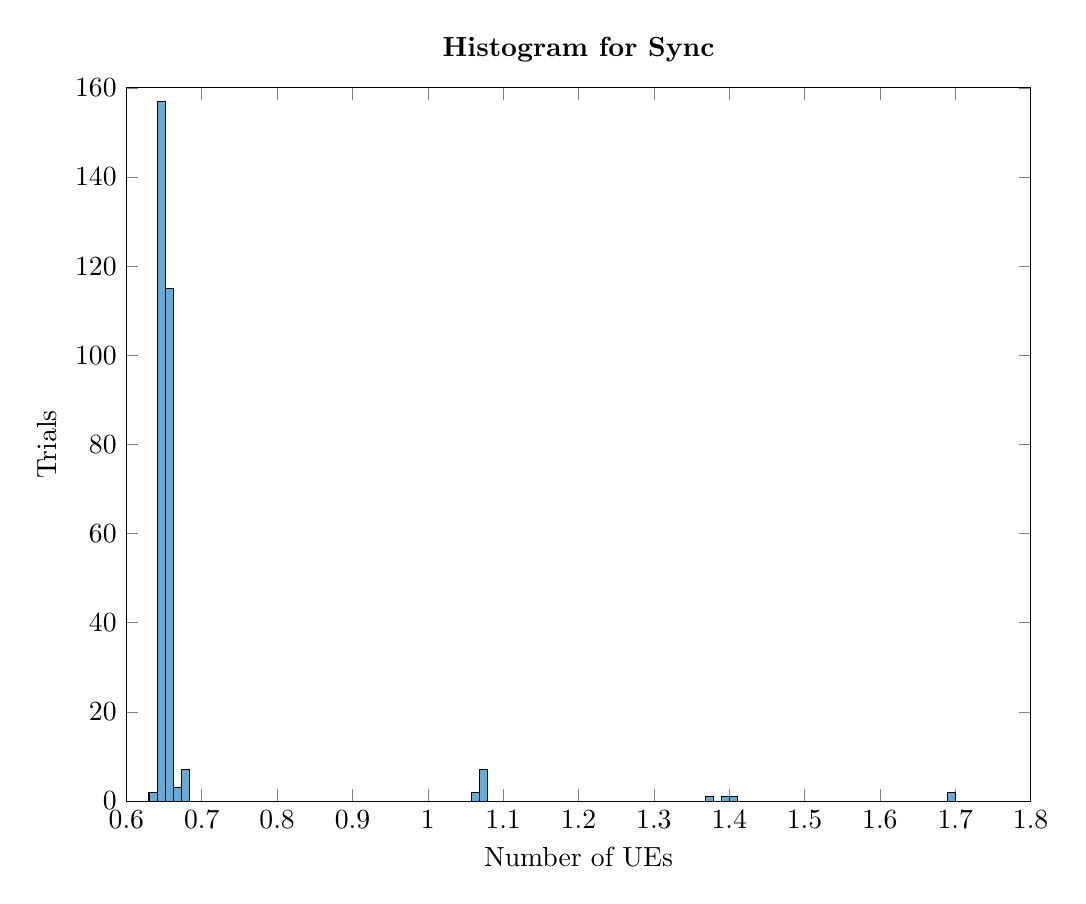
\begin{tikzpicture}

\begin{axis}[%
width=4.521in,
height=3.566in,
at={(0.758in,0.481in)},
scale only axis,
xmin=0.6,
xmax=1.8,
xlabel={Number of UEs},
ymin=0,
ymax=160,
ylabel={Trials},
axis background/.style={fill=white},
title style={font=\bfseries},
title={Histogram for Sync}
]
\addplot[fill=mycolor1,fill opacity=0.6,draw=black,ybar interval,area legend] plot table[row sep=crcr] {%
x	y\\
0.63	2\\
0.6407	157\\
0.6514	115\\
0.6621	3\\
0.6728	7\\
0.6835	0\\
0.6942	0\\
0.7049	0\\
0.7156	0\\
0.7263	0\\
0.737	0\\
0.7477	0\\
0.7584	0\\
0.7691	0\\
0.7798	0\\
0.7905	0\\
0.8012	0\\
0.8119	0\\
0.8226	0\\
0.8333	0\\
0.844	0\\
0.8547	0\\
0.8654	0\\
0.8761	0\\
0.8868	0\\
0.8975	0\\
0.9082	0\\
0.9189	0\\
0.9296	0\\
0.9403	0\\
0.951	0\\
0.9617	0\\
0.9724	0\\
0.9831	0\\
0.9938	0\\
1.0045	0\\
1.0152	0\\
1.0259	0\\
1.0366	0\\
1.0473	0\\
1.058	2\\
1.0687	7\\
1.0794	0\\
1.0901	0\\
1.1008	0\\
1.1115	0\\
1.1222	0\\
1.1329	0\\
1.1436	0\\
1.1543	0\\
1.165	0\\
1.1757	0\\
1.1864	0\\
1.1971	0\\
1.2078	0\\
1.2185	0\\
1.2292	0\\
1.2399	0\\
1.2506	0\\
1.2613	0\\
1.272	0\\
1.2827	0\\
1.2934	0\\
1.3041	0\\
1.3148	0\\
1.3255	0\\
1.3362	0\\
1.3469	0\\
1.3576	0\\
1.3683	1\\
1.379	0\\
1.3897	1\\
1.4004	1\\
1.4111	0\\
1.4218	0\\
1.4325	0\\
1.4432	0\\
1.4539	0\\
1.4646	0\\
1.4753	0\\
1.486	0\\
1.4967	0\\
1.5074	0\\
1.5181	0\\
1.5288	0\\
1.5395	0\\
1.5502	0\\
1.5609	0\\
1.5716	0\\
1.5823	0\\
1.593	0\\
1.6037	0\\
1.6144	0\\
1.6251	0\\
1.6358	0\\
1.6465	0\\
1.6572	0\\
1.6679	0\\
1.6786	0\\
1.6893	2\\
1.7	2\\
};
\end{axis}
\end{tikzpicture}%}
\caption{The distribution for the execution time for synchronization for all different number of devices.}
\label{fig:MT_Sync_His}
\end{figure}
\end{minipage}
\captionsetup{belowskip=-1.5em}

As seen on \autoref{fig:MT_Sync_Time} is the execution time for different number of devices is behaving equal to each other. Another aspect seen on the figure is that some measurements have taken some extra time to execute, but is aligning at the same time values, which also indicated on the histogram on \autoref{fig:MT_Sync_His}. Here it is seen that most measurements is placed at 0.6 s to 0.8 s and the amount at the other points is much lower. This is to be expected as the structure of the MDE only searches for the cell once independently of the number of devices.



\subsection{MIB-NB decoding}
The execution time for the MIB-NB decoding step is measured from just after a cell is found until the MIB-NB has been fully decoded, which gives the results seen on \autoref{fig:MT_MIB_Time}. However as the MDE sometimes fails, which results in it retrying the decoding, a bias is made to only use the time for the final and successful decoding of MIB-NB.


\captionsetup{belowskip=0em}
\begin{minipage}{0.48\textwidth}
\begin{figure}[H]
\tikzsetnextfilename{MT_MIB_Time}
\centering
\resizebox{\textwidth}{!}{
% This file was created by matlab2tikz.
%
%The latest updates can be retrieved from
%  http://www.mathworks.com/matlabcentral/fileexchange/22022-matlab2tikz-matlab2tikz
%where you can also make suggestions and rate matlab2tikz.
%
\definecolor{mycolor1}{rgb}{0.00000,0.44700,0.74100}%
\definecolor{mycolor2}{rgb}{0.85000,0.32500,0.09800}%
%
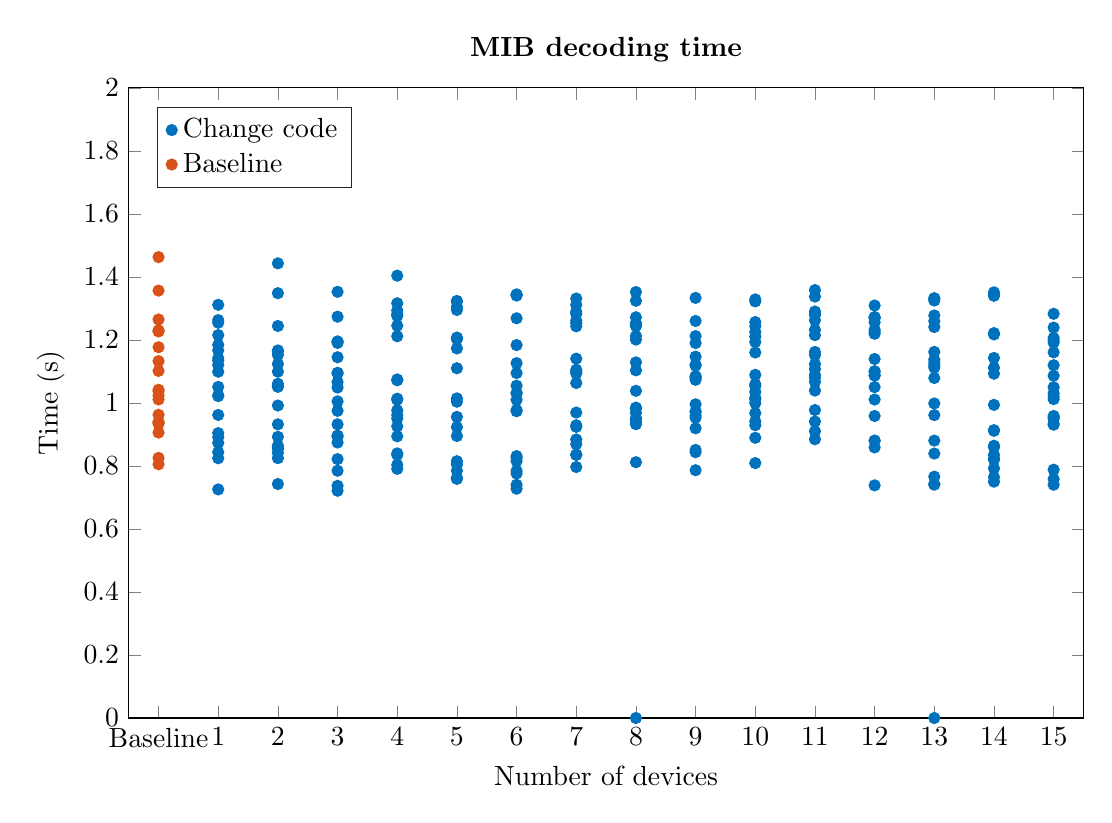
\begin{tikzpicture}

\begin{axis}[%
width=\textwidth,
height=.66\textwidth,
at={(0.758in,0.481in)},
scale only axis,
xmin=-0.5,
xmax=15.5,
xtick={0,1,2,3,4,5,6,7,8,9,10,11,12,13,14,15},
xticklabels={{Baseline},{1},{2},{3},{4},{5},{6},{7},{8},{9},{10},{11},{12},{13},{14},{15}},
xlabel={Number of devices},
ymin=0,
ymax=2,
ylabel={Time (s)},
axis background/.style={fill=white},
title style={font=\bfseries},
title={MIB decoding time},
legend style={at={(0.03,0.97)},anchor=north west,legend cell align=left,align=left,draw=white!15!black}
]
\addplot [color=mycolor1,only marks,mark=*,mark options={solid}]
  table[row sep=crcr]{%
1	1.18452787399292\\
1	1.02464199066162\\
1	1.16689705848694\\
1	0.904258966445923\\
1	0.843533992767334\\
1	1.13420486450195\\
1	0.824519872665405\\
1	0.961822032928467\\
1	0.891458988189697\\
1	1.3114321231842\\
1	0.72556209564209\\
1	1.26286196708679\\
1	1.25451898574829\\
1	1.12048602104187\\
1	1.02167701721191\\
1	1.09917998313904\\
1	0.873126983642578\\
1	1.14201807975769\\
1	1.21537899971008\\
1	1.05097317695618\\
};
\addlegendentry{Change code};

\addplot [color=mycolor1,only marks,mark=*,mark options={solid},forget plot]
  table[row sep=crcr]{%
2	0.742633819580078\\
2	1.12349700927734\\
2	0.862571001052856\\
2	1.09928011894226\\
2	1.06075310707092\\
2	0.841415166854858\\
2	0.824921131134033\\
2	1.05261611938477\\
2	1.0511691570282\\
2	1.34838080406189\\
2	1.16666889190674\\
2	0.892491817474365\\
2	0.863969087600708\\
2	0.991780996322632\\
2	1.16264510154724\\
2	1.15249800682068\\
2	1.24425196647644\\
2	0.853885173797607\\
2	1.44308090209961\\
2	0.932136058807373\\
};


\addplot [color=mycolor1,only marks,mark=*,mark options={solid},forget plot]
  table[row sep=crcr]{%
3	1.35272288322449\\
3	0.896404027938843\\
3	1.19529414176941\\
3	0.721312999725342\\
3	1.00501799583435\\
3	0.974997997283936\\
3	1.27371096611023\\
3	1.09565401077271\\
3	1.19446611404419\\
3	0.736949920654297\\
3	0.784852981567383\\
3	0.874388933181763\\
3	0.932243824005127\\
3	0.821744918823242\\
3	1.09404897689819\\
3	1.14502000808716\\
3	0.893469095230103\\
3	1.19056606292725\\
3	1.06648683547974\\
3	1.04886889457703\\
};
\addplot [color=mycolor1,only marks,mark=*,mark options={solid},forget plot]
  table[row sep=crcr]{%
4	1.21173596382141\\
4	0.894090890884399\\
4	0.950580835342407\\
4	1.31642508506775\\
4	0.83543586730957\\
4	0.925927877426147\\
4	0.976491928100586\\
4	1.28235483169556\\
4	0.803546905517578\\
4	0.790771007537842\\
4	1.27620601654053\\
4	1.01348495483398\\
4	1.07200884819031\\
4	1.01012992858887\\
4	0.839915037155151\\
4	0.962180137634277\\
4	1.07453393936157\\
4	1.29357409477234\\
4	1.40396094322205\\
4	1.24524092674255\\
};
\addplot [color=mycolor1,only marks,mark=*,mark options={solid},forget plot]
  table[row sep=crcr]{%
5	1.29511213302612\\
5	1.01446914672852\\
5	1.20752096176147\\
5	1.20313382148743\\
5	0.805004119873047\\
5	1.30468487739563\\
5	0.815110921859741\\
5	0.758973121643066\\
5	1.11016798019409\\
5	0.761851072311401\\
5	0.955629825592041\\
5	1.00391411781311\\
5	1.32148098945618\\
5	1.17293000221252\\
5	0.923401832580566\\
5	0.895086050033569\\
5	1.20391082763672\\
5	0.76114296913147\\
5	0.784970045089722\\
5	1.32375192642212\\
};
\addplot [color=mycolor1,only marks,mark=*,mark options={solid},forget plot]
  table[row sep=crcr]{%
6	1.12626886367798\\
6	0.784417867660522\\
6	0.973766088485718\\
6	1.34400105476379\\
6	1.03182911872864\\
6	1.00979208946228\\
6	1.18366503715515\\
6	0.977426052093506\\
6	0.831204891204834\\
6	1.34424090385437\\
6	1.26865386962891\\
6	0.815386056900024\\
6	0.72773003578186\\
6	1.09482884407043\\
6	0.776089191436768\\
6	1.34079313278198\\
6	0.740194082260132\\
6	0.825405120849609\\
6	1.03018093109131\\
6	1.05475306510925\\
};
\addplot [color=mycolor1,only marks,mark=*,mark options={solid},forget plot]
  table[row sep=crcr]{%
7	1.14058113098145\\
7	0.969480037689209\\
7	1.2895450592041\\
7	1.25373196601868\\
7	0.869355916976929\\
7	0.836460828781128\\
7	0.883985042572021\\
7	1.33135199546814\\
7	1.10523915290833\\
7	1.06331515312195\\
7	0.834944009780884\\
7	0.796628952026367\\
7	1.09889316558838\\
7	1.26145696640015\\
7	1.31127190589905\\
7	0.929186105728149\\
7	1.09361791610718\\
7	0.924177885055542\\
7	1.28277397155762\\
7	1.24324703216553\\
};
\addplot [color=mycolor1,only marks,mark=*,mark options={solid},forget plot]
  table[row sep=crcr]{%
8	1.21215677261353\\
8	0.811891078948975\\
8	1.35208201408386\\
8	1.25351810455322\\
8	1.24444103240967\\
8	0.96881103515625\\
8	1.32427191734314\\
8	1.24557089805603\\
8	0.985246181488037\\
8	1.10344481468201\\
8	0.947085857391357\\
8	1.03846478462219\\
8	0.940639019012451\\
8	1.27187204360962\\
8	0.932521820068359\\
8	1.20112204551697\\
8	0.952279090881348\\
8	0.981828927993774\\
8	1.12882900238037\\
8	0\\
};
\addplot [color=mycolor1,only marks,mark=*,mark options={solid},forget plot]
  table[row sep=crcr]{%
9	1.07991504669189\\
9	1.19017219543457\\
9	1.26013112068176\\
9	1.21215891838074\\
9	0.786477088928223\\
9	1.14683389663696\\
9	0.953114032745361\\
9	0.919471025466919\\
9	1.3333580493927\\
9	1.07340693473816\\
9	0.95987606048584\\
9	0.84372091293335\\
9	0.995597839355469\\
9	1.08392119407654\\
9	0.971073150634766\\
9	1.1183009147644\\
9	1.08447599411011\\
9	0.850917100906372\\
9	0.973115921020508\\
9	1.12152695655823\\
};
\addplot [color=mycolor1,only marks,mark=*,mark options={solid},forget plot]
  table[row sep=crcr]{%
10	1.25671696662903\\
10	1.05311989784241\\
10	0.929455041885376\\
10	1.19342279434204\\
10	1.05944609642029\\
10	1.01689720153809\\
10	0.967733860015869\\
10	1.21085119247437\\
10	1.22501087188721\\
10	1.08909916877747\\
10	0.941591024398804\\
10	1.1600980758667\\
10	1.24331402778625\\
10	0.889430046081543\\
10	1.32221412658691\\
10	1.01067590713501\\
10	0.999495983123779\\
10	1.3286120891571\\
10	1.03497505187988\\
10	0.809139966964722\\
};
\addplot [color=mycolor1,only marks,mark=*,mark options={solid},forget plot]
  table[row sep=crcr]{%
11	0.941027879714966\\
11	1.35822701454163\\
11	0.977467060089111\\
11	1.29018783569336\\
11	1.10762286186218\\
11	1.12313294410706\\
11	1.08049416542053\\
11	1.08900213241577\\
11	1.15175604820251\\
11	1.06713485717773\\
11	1.1618390083313\\
11	1.21526479721069\\
11	1.33760190010071\\
11	0.884803056716919\\
11	1.23175096511841\\
11	0.910167932510376\\
11	1.27922487258911\\
11	1.03915095329285\\
11	1.28432893753052\\
11	1.26249885559082\\
};
\addplot [color=mycolor1,only marks,mark=*,mark options={solid},forget plot]
  table[row sep=crcr]{%
12	0.858820915222168\\
12	1.21957588195801\\
12	0.880445003509521\\
12	1.05029010772705\\
12	1.23261284828186\\
12	1.30926299095154\\
12	0.879901170730591\\
12	1.27121210098267\\
12	1.13944888114929\\
12	0.958610057830811\\
12	1.08663201332092\\
12	1.01077389717102\\
12	1.08854699134827\\
12	1.2690908908844\\
12	1.22531986236572\\
12	1.09908199310303\\
12	1.27269697189331\\
12	1.25594997406006\\
12	1.10074591636658\\
12	0.738483905792236\\
};
\addplot [color=mycolor1,only marks,mark=*,mark options={solid},forget plot]
  table[row sep=crcr]{%
13	0.83938193321228\\
13	0.998347997665405\\
13	1.32503414154053\\
13	0.880541086196899\\
13	1.16189002990723\\
13	0.742758989334106\\
13	0.765993118286133\\
13	1.25955986976624\\
13	1.0792031288147\\
13	0.740605115890503\\
13	1.33235692977905\\
13	1.11989402770996\\
13	1.13771796226501\\
13	1.11200213432312\\
13	1.1292519569397\\
13	0.961405992507935\\
13	1.27758502960205\\
13	1.24095487594604\\
13	1.33164381980896\\
13	0\\
};
\addplot [color=mycolor1,only marks,mark=*,mark options={solid},forget plot]
  table[row sep=crcr]{%
14	0.835340976715088\\
14	1.21743702888489\\
14	1.1116509437561\\
14	0.764328956604004\\
14	1.3510730266571\\
14	1.34011006355286\\
14	0.861910104751587\\
14	1.09282898902893\\
14	1.14283895492554\\
14	1.34170484542847\\
14	0.792457103729248\\
14	0.864109992980957\\
14	0.750169038772583\\
14	1.22165703773499\\
14	0.819968938827515\\
14	0.823435068130493\\
14	0.993892908096313\\
14	0.913672924041748\\
14	0.91166090965271\\
14	0.859905958175659\\
};
\addplot [color=mycolor1,only marks,mark=*,mark options={solid},forget plot]
  table[row sep=crcr]{%
15	0.958617925643921\\
15	1.01214718818665\\
15	1.23916387557983\\
15	0.954987049102783\\
15	1.02038717269897\\
15	0.949368000030518\\
15	1.08639097213745\\
15	1.20632886886597\\
15	1.28288388252258\\
15	1.04977297782898\\
15	0.788140058517456\\
15	0.933758020401001\\
15	1.16064596176147\\
15	0.740518093109131\\
15	1.11970591545105\\
15	1.19137382507324\\
15	0.931004047393799\\
15	0.758590936660767\\
15	1.19861912727356\\
15	1.03083515167236\\
};
\addplot [color=mycolor2,only marks,mark=*,mark options={solid}]
  table[row sep=crcr]
\caption{Execution time for the decoding the MIB-NB for different number of devices and the baseline emulator. A single measurement for the base line is placed at 5.0834 s, which is not shown on this figure.}
\label{fig:MT_MIB_Time}
\end{figure}
\end{minipage}%
\hfill
\begin{minipage}{0.48\textwidth}
\begin{figure}[H]
\tikzsetnextfilename{MT_MIB_His}
\centering
\resizebox{\textwidth}{!}{
% This file was created by matlab2tikz.
%
%The latest updates can be retrieved from
%  http://www.mathworks.com/matlabcentral/fileexchange/22022-matlab2tikz-matlab2tikz
%where you can also make suggestions and rate matlab2tikz.
%
\definecolor{mycolor1}{rgb}{0.00000,0.44700,0.74100}%
%
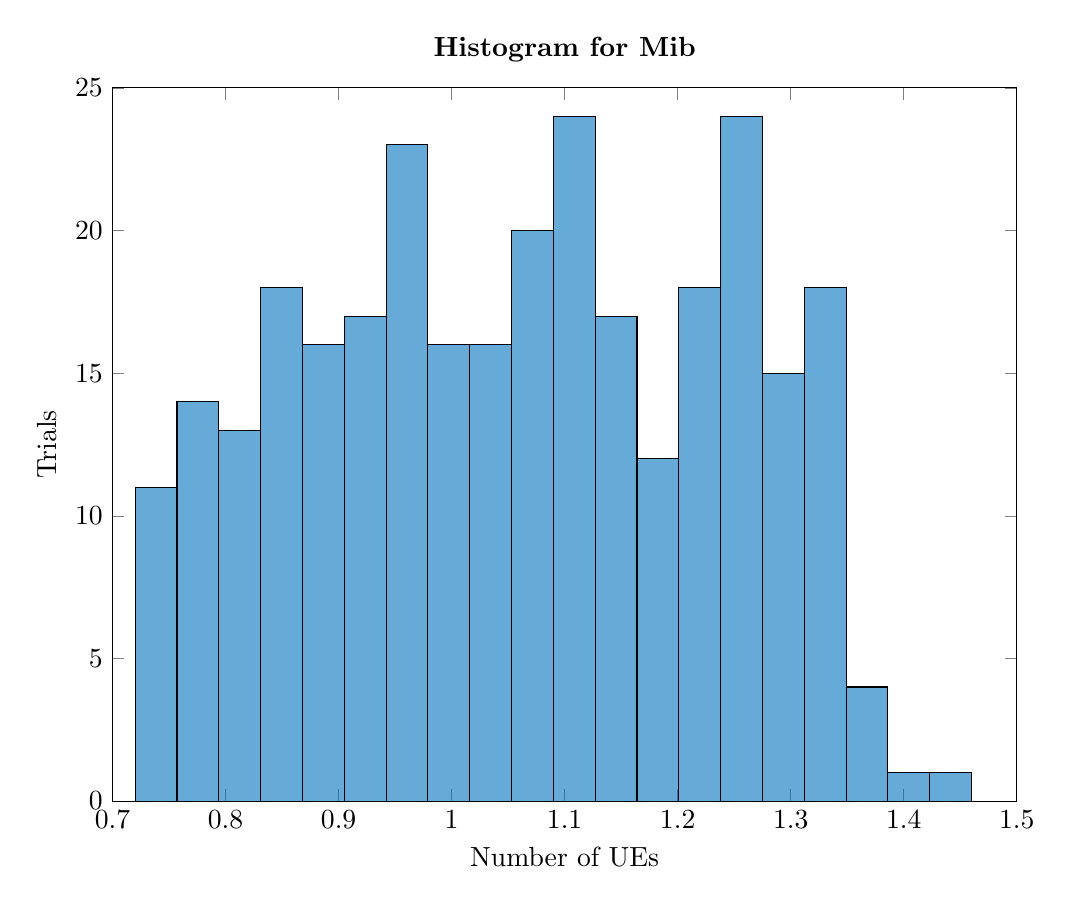
\begin{tikzpicture}

\begin{axis}[%
width=4.521in,
height=3.566in,
at={(0.758in,0.481in)},
scale only axis,
xmin=0.7,
xmax=1.5,
xlabel={Number of UEs},
ymin=0,
ymax=25,
ylabel={Trials},
axis background/.style={fill=white},
title style={font=\bfseries},
title={Histogram for Mib}
]
\addplot[fill=mycolor1,fill opacity=0.6,draw=black,ybar interval,area legend] plot table[row sep=crcr] 
\caption{The distribution for the execution time for decoding the MIB-NB for all different number of devices.}
\label{fig:MT_MIB_His}
\end{figure}
\end{minipage}
\captionsetup{belowskip=-1.5em}

As seen on \autoref{fig:MT_MIB_Time} the execution time for the MIB-NB decoding quite stable independently on the number of devices. The spread is big compared to the synchronazitation step, which also can be seen when comparing the histogram for the two steps, \autoref{fig:MT_Sync_His} and \autoref{fig:MT_MIB_His}. The baseline emulator have the same tendency as the MDE, which indicates that the changes do not effect this step, as expected. On \autoref{fig:MT_MIB_Tries} is it shown how many attempts the different measurements needed before completing the MIB-NB decoding step.

\begin{figure}[H]
\tikzsetnextfilename{MT_MIB_Tries}
\centering
%\resizebox{0.5\textwidth}{!}{
% This file was created by matlab2tikz.
%
%The latest updates can be retrieved from
%  http://www.mathworks.com/matlabcentral/fileexchange/22022-matlab2tikz-matlab2tikz
%where you can also make suggestions and rate matlab2tikz.
%
\definecolor{mycolor1}{rgb}{0.20810,0.16630,0.52920}%
\definecolor{mycolor2}{rgb}{0.02650,0.61370,0.81350}%
\definecolor{mycolor3}{rgb}{0.64730,0.74560,0.41880}%
\definecolor{mycolor4}{rgb}{0.97630,0.98310,0.05380}%
%
\begin{tikzpicture}

\begin{axis}[%
width=0.5\textwidth,
height=.33\textwidth,
at={(0.607in,0.481in)},
scale only axis,
bar width=0.5,
xmin=-0.5,
xmax=15.5,
xtick={0,1,2,3,4,5,6,7,8,9,10,11,12,13,14,15},
xticklabels={{Base},{1},{2},{3},{4},{5},{6},{7},{8},{9},{10},{11},{12},{13},{14},{15}},
xlabel={Number of devices},
ymin=0,
ymax=1,
ylabel={Trials},
axis background/.style={fill=white},
title style={font=\bfseries},
title={Number of tries for decoding MIB},
legend style={at={(1.03,1)},anchor=north west,legend cell align=left,align=left,draw=white!15!black}
]
\addplot[ybar stacked,draw=black,fill=mycolor1,area legend] plot table[row sep=crcr] {%
0	0.65\\
1	0.8\\
2	0.85\\
3	0.75\\
4	0.9\\
5	0.65\\
6	0.85\\
7	0.85\\
8	0.736842105263158\\
9	0.9\\
10	0.95\\
11	0.95\\
12	1\\
13	0.842105263157895\\
14	0.95\\
15	0.95\\
};
\addlegendentry{1 Attempts};

\addplot[ybar stacked,draw=black,fill=mycolor2,area legend] plot table[row sep=crcr] {%
0	0.25\\
1	0.15\\
2	0.05\\
3	0.2\\
4	0.1\\
5	0.25\\
6	0\\
7	0.15\\
8	0.263157894736842\\
9	0.1\\
10	0.05\\
11	0.05\\
12	0\\
13	0.157894736842105\\
14	0.05\\
15	0.05\\
};
\addlegendentry{2 Attempts};

\addplot[ybar stacked,draw=black,fill=mycolor3,area legend] plot table[row sep=crcr] {%
0	0.1\\
1	0.05\\
2	0.05\\
3	0.05\\
4	0\\
5	0.05\\
6	0.15\\
7	0\\
8	0\\
9	0\\
10	0\\
11	0\\
12	0\\
13	0\\
14	0\\
15	0\\
};
\addlegendentry{3 Attempts};

\addplot[ybar stacked,draw=black,fill=mycolor4,area legend] plot table[row sep=crcr] {%
0	0\\
1	0\\
2	0.05\\
3	0\\
4	0\\
5	0.05\\
6	0\\
7	0\\
8	0\\
9	0\\
10	0\\
11	0\\
12	0\\
13	0\\
14	0\\
15	0\\
};
\addlegendentry{4 Attempts};

\end{axis}
\end{tikzpicture}%
\caption{The distribution for number of attempts for decoding the MIB-NB for different number of devices.}
\label{fig:MT_MIB_Tries}
\end{figure}

It is seen on \autoref{fig:MT_MIB_Tries} that baseline emulator is not different from the MDE at a lower number of devices. At a higher number of devices it even seems like the MDE is more efficient, as the failed attempts decreases when the number of devices increases.

\subsection{NB-SIB1}
The execution time for the NB-SIB1 decoding step is measured from the MIB-NB is decoded to the NB-SIB1 is fully decoded, which gives the results seen on \autoref{fig:MT_SIB1_Time}. The test is executed with the different number of devices, but the results shown on \autoref{fig:MT_SIB1_Time} is only for one of the emulated devices, as each device demodulates the NB-SIB1 individually. This is done, so all number of devices have the same stand point compared to the measurements.
As both the radio error and idle after MIB-NB error occurs in this step of the process, the number of measurement points are lowered further.

\captionsetup{belowskip=0em}
\begin{minipage}{0.48\textwidth}
\begin{figure}[H]
\tikzsetnextfilename{MT_SIB1_Time}
\centering
\resizebox{\textwidth}{!}{
% This file was created by matlab2tikz.
%
%The latest updates can be retrieved from
%  http://www.mathworks.com/matlabcentral/fileexchange/22022-matlab2tikz-matlab2tikz
%where you can also make suggestions and rate matlab2tikz.
%
\definecolor{mycolor1}{rgb}{0.00000,0.44700,0.74100}%
\definecolor{mycolor2}{rgb}{0.85000,0.32500,0.09800}%
%
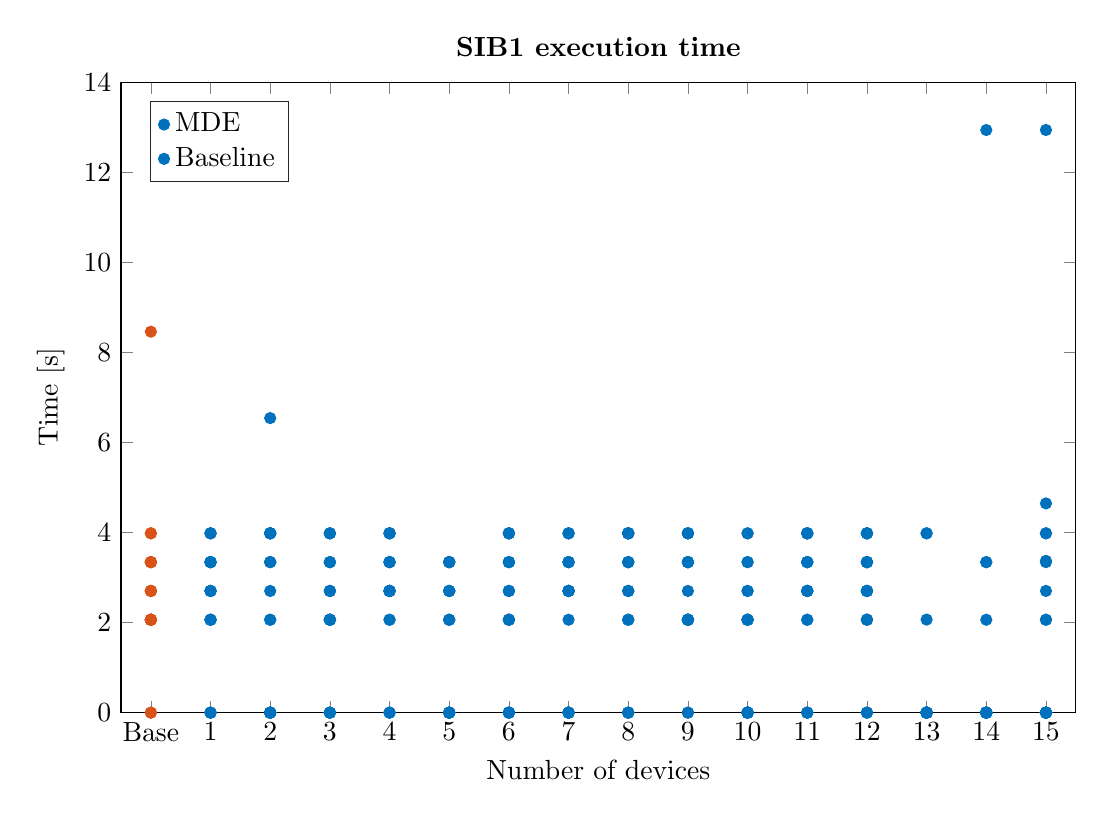
\begin{tikzpicture}

\begin{axis}[%
width=\textwidth,
height=.66\textwidth,
at={(0.758in,0.481in)},
scale only axis,
xmin=-0.5,
xmax=15.5,
xtick={0,1,2,3,4,5,6,7,8,9,10,11,12,13,14,15},
xticklabels={{Base},{1},{2},{3},{4},{5},{6},{7},{8},{9},{10},{11},{12},{13},{14},{15}},
xlabel={Number of devices},
ymin=0,
ymax=14,
ylabel={Time [s]},
axis background/.style={fill=white},
title style={font=\bfseries},
title={SIB1 execution time},
legend style={at={(0.03,0.97)},anchor=north west,legend cell align=left,align=left,draw=white!15!black}
]
\addplot [color=mycolor1,only marks,mark=*,mark options={solid}]
  table[row sep=crcr]{%
1	2.06326198577881\\
1	2.06440305709839\\
1	3.98324704170227\\
1	3.34370994567871\\
1	2.064288854599\\
1	2.06284713745117\\
1	3.34417414665222\\
1	0\\
1	3.98412108421326\\
1	0\\
1	0\\
1	3.34290599822998\\
1	3.98381996154785\\
1	2.70346093177795\\
1	2.7038140296936\\
1	3.34348487854004\\
1	2.70364594459534\\
1	3.34404802322388\\
1	2.70409893989563\\
1	0\\
};
\addlegendentry{MDE};

\addplot [color=mycolor1,only marks,mark=*,mark options={solid},forget plot]
  table[row sep=crcr]{%
2	0\\
2	2.06386804580688\\
2	3.9830470085144\\
2	2.70327496528625\\
2	3.98435401916504\\
2	3.34425902366638\\
2	0\\
2	0\\
2	3.34448194503784\\
2	3.98420310020447\\
2	3.98417806625366\\
2	0\\
2	0\\
2	0\\
2	2.06371593475342\\
2	0\\
2	3.98412013053894\\
2	6.54380798339844\\
2	3.34428119659424\\
2	0\\
};

\addplot [color=mycolor1,only marks,mark=*,mark options={solid}]
  table[row sep=crcr]{%
3	0\\
3	3.34311699867249\\
3	2.06403684616089\\
3	2.06435298919678\\
3	2.06442618370056\\
3	3.98329901695251\\
3	0\\
3	2.06374597549438\\
3	3.98314690589905\\
3	2.70358204841614\\
3	3.34318780899048\\
3	3.98370504379272\\
3	0\\
3	2.70299601554871\\
3	0\\
3	0\\
3	3.34412288665771\\
3	2.70408582687378\\
3	2.06382894515991\\
3	2.06484198570251\\
};
\addplot [color=mycolor1,only marks,mark=*,mark options={solid},forget plot]
  table[row sep=crcr]{%
4	3.34450602531433\\
4	2.70465612411499\\
4	3.9842541217804\\
4	0\\
4	0\\
4	2.70361804962158\\
4	3.34443497657776\\
4	3.3442051410675\\
4	3.98412203788757\\
4	0\\
4	2.70440602302551\\
4	2.70354795455933\\
4	3.98445606231689\\
4	3.34337210655212\\
4	2.7031729221344\\
4	2.06350088119507\\
4	2.7041220664978\\
4	3.98393082618713\\
4	2.7035870552063\\
4	2.06354808807373\\
};
\addplot [color=mycolor1,only marks,mark=*,mark options={solid},forget plot]
  table[row sep=crcr]{%
5	2.70302295684814\\
5	2.0638120174408\\
5	2.70368385314941\\
5	3.34371113777161\\
5	3.34336185455322\\
5	0\\
5	0\\
5	2.06377196311951\\
5	3.34426617622375\\
5	0\\
5	0\\
5	2.06288194656372\\
5	2.70433521270752\\
5	2.70352816581726\\
5	0\\
5	0\\
5	0\\
5	0\\
5	3.34436511993408\\
5	3.34376907348633\\
};
\addplot [color=mycolor1,only marks,mark=*,mark options={solid},forget plot]
  table[row sep=crcr]{%
6	2.70398306846619\\
6	3.98413896560669\\
6	2.70379996299744\\
6	2.06457901000977\\
6	3.34415984153748\\
6	2.06386399269104\\
6	0\\
6	3.98335313796997\\
6	2.06371712684631\\
6	3.34421420097351\\
6	3.98331713676453\\
6	0\\
6	3.98413610458374\\
6	2.06382918357849\\
6	0\\
6	3.34377503395081\\
6	0\\
6	0\\
6	3.34429097175598\\
6	2.70383501052856\\
};
\addplot [color=mycolor1,only marks,mark=*,mark options={solid},forget plot]
  table[row sep=crcr]{%
7	2.70354390144348\\
7	0\\
7	2.70460295677185\\
7	3.34423208236694\\
7	0\\
7	2.70423698425293\\
7	2.06377696990967\\
7	0\\
7	0\\
7	0\\
7	3.98403000831604\\
7	3.34456205368042\\
7	3.98315095901489\\
7	3.34323811531067\\
7	2.70326495170593\\
7	3.34363293647766\\
7	0\\
7	2.70313405990601\\
7	3.98417210578918\\
7	2.70344686508179\\
};
\addplot [color=mycolor1,only marks,mark=*,mark options={solid},forget plot]
  table[row sep=crcr]{%
8	3.34394001960754\\
8	3.9837920665741\\
8	3.98305892944336\\
8	2.06428194046021\\
8	0\\
8	2.06423997879028\\
8	3.9834680557251\\
8	0\\
8	2.70423197746277\\
8	3.34431982040405\\
8	0\\
8	2.7035391330719\\
8	0\\
8	3.34361791610718\\
8	2.06392502784729\\
8	3.98410606384277\\
8	2.70362114906311\\
8	3.34315776824951\\
8	3.98356890678406\\
8	3.98443794250488\\
};
\addplot [color=mycolor1,only marks,mark=*,mark options={solid},forget plot]
  table[row sep=crcr]{%
9	2.06394577026367\\
9	3.34412384033203\\
9	3.98399186134338\\
9	3.9841251373291\\
9	2.06348896026611\\
9	0\\
9	3.34316611289978\\
9	2.06286597251892\\
9	3.98410415649414\\
9	2.06404900550842\\
9	2.06381487846375\\
9	2.06389117240906\\
9	0\\
9	2.06410598754883\\
9	2.70342183113098\\
9	3.34323501586914\\
9	3.34321093559265\\
9	3.98393988609314\\
9	2.06367611885071\\
9	3.34430599212646\\
};
\addplot [color=mycolor1,only marks,mark=*,mark options={solid},forget plot]
  table[row sep=crcr]{%
10	0\\
10	3.98293900489807\\
10	3.34414911270142\\
10	2.06450819969177\\
10	0\\
10	0\\
10	0\\
10	3.34374499320984\\
10	0\\
10	0\\
10	3.98308205604553\\
10	2.06371092796326\\
10	2.06403684616089\\
10	2.06367516517639\\
10	0\\
10	2.7036759853363\\
10	2.06395602226257\\
10	2.70334911346436\\
10	0\\
10	0\\
};
\addplot [color=mycolor1,only marks,mark=*,mark options={solid},forget plot]
  table[row sep=crcr]{%
11	3.34377312660217\\
11	2.70394802093506\\
11	2.7042019367218\\
11	3.98395895957947\\
11	0\\
11	3.34369802474976\\
11	2.70436382293701\\
11	2.70322489738464\\
11	3.34422206878662\\
11	2.70361518859863\\
11	3.98409199714661\\
11	3.34430408477783\\
11	0\\
11	3.98311901092529\\
11	3.98332715034485\\
11	2.06374907493591\\
11	0\\
11	0\\
11	3.98366022109985\\
11	2.06314301490784\\
};
\addplot [color=mycolor1,only marks,mark=*,mark options={solid},forget plot]
  table[row sep=crcr]{%
12	2.7039110660553\\
12	2.06496000289917\\
12	2.70287799835205\\
12	2.7045431137085\\
12	3.98310804367065\\
12	2.70452785491943\\
12	3.34418082237244\\
12	0\\
12	3.98356199264526\\
12	0\\
12	3.34408807754517\\
12	3.34393095970154\\
12	3.98390102386475\\
12	0\\
12	3.98423719406128\\
12	3.34313797950745\\
12	2.70388698577881\\
12	3.34319090843201\\
12	2.06460905075073\\
12	2.06348609924316\\
};
\addplot [color=mycolor1,only marks,mark=*,mark options={solid},forget plot]
  table[row sep=crcr]{%
13	0\\
13	0\\
13	0\\
13	0\\
13	3.98369693756104\\
13	0\\
13	0\\
13	0\\
13	0\\
13	0\\
13	0\\
13	0\\
13	0\\
13	0\\
13	3.98429584503174\\
13	0\\
13	0\\
13	0\\
13	0\\
13	2.06700801849365\\
};
\addplot [color=mycolor1,only marks,mark=*,mark options={solid},forget plot]
  table[row sep=crcr]{%
14	0\\
14	2.06355404853821\\
14	0\\
14	0\\
14	0\\
14	0\\
14	0\\
14	3.34336185455322\\
14	0\\
14	0\\
14	3.34429407119751\\
14	0\\
14	0\\
14	0\\
14	0\\
14	0\\
14	12.9436860084534\\
14	0\\
14	0\\
14	0\\
};
\addplot [color=mycolor1,only marks,mark=*,mark options={solid},forget plot]
  table[row sep=crcr]{%
15	3.37162494659424\\
15	0\\
15	2.06366395950317\\
15	2.70392298698425\\
15	0\\
15	3.98395490646362\\
15	0\\
15	12.9445569515228\\
15	0\\
15	0\\
15	0\\
15	0\\
15	3.34374690055847\\
15	0\\
15	3.98381996154785\\
15	4.64827418327332\\
15	0\\
15	2.06406998634338\\
15	0\\
15	0\\
};
\addplot [color=mycolor2,only marks,mark=*,mark options={solid}]
  table[row sep=crcr]
\caption{Execution time for the decoding the NB-SIB1 step for different number of devices and the baseline emulator.}
\label{fig:MT_SIB1_Time}
\end{figure}
\end{minipage}%
\hfill
\begin{minipage}{0.48\textwidth}
\begin{figure}[H]
\tikzsetnextfilename{MT_SIB1_His}
\centering
\resizebox{\textwidth}{!}{
% This file was created by matlab2tikz.
%
%The latest updates can be retrieved from
%  http://www.mathworks.com/matlabcentral/fileexchange/22022-matlab2tikz-matlab2tikz
%where you can also make suggestions and rate matlab2tikz.
%
\definecolor{mycolor1}{rgb}{0.00000,0.44700,0.74100}%
%
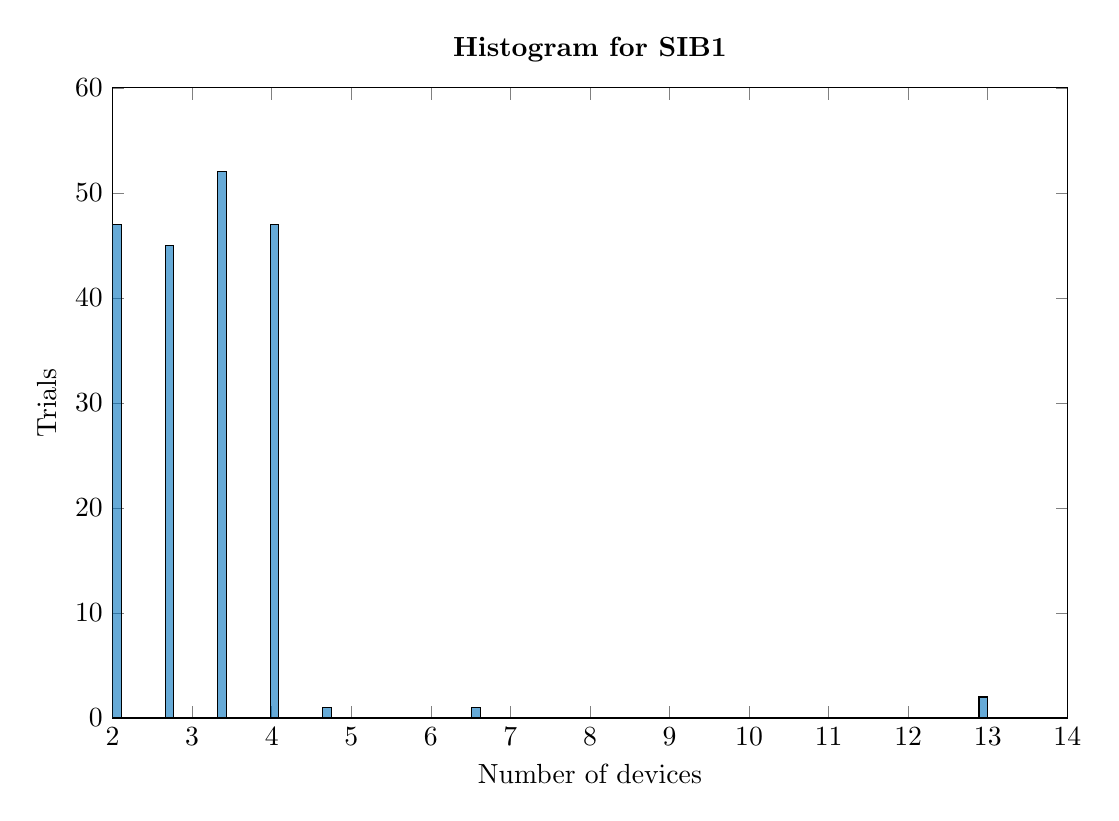
\begin{tikzpicture}

\begin{axis}[%
width=\textwidth,
height=0.66\textwidth,
at={(0.758in,0.481in)},
scale only axis,
xmin=2,
xmax=14,
xlabel={Number of devices},
ymin=0,
ymax=60,
ylabel={Trials},
axis background/.style={fill=white},
title style={font=\bfseries},
title={Histogram for SIB1}
]
\addplot[fill=mycolor1,fill opacity=0.6,draw=black,ybar interval,area legend] plot table[row sep=crcr] {%
x	y\\
2	47\\
2.11	0\\
2.22	0\\
2.33	0\\
2.44	0\\
2.55	0\\
2.66	45\\
2.77	0\\
2.88	0\\
2.99	0\\
3.1	0\\
3.21	0\\
3.32	52\\
3.43	0\\
3.54	0\\
3.65	0\\
3.76	0\\
3.87	0\\
3.98	47\\
4.09	0\\
4.2	0\\
4.31	0\\
4.42	0\\
4.53	0\\
4.64	1\\
4.75	0\\
4.86	0\\
4.97	0\\
5.08	0\\
5.19	0\\
5.3	0\\
5.41	0\\
5.52	0\\
5.63	0\\
5.74	0\\
5.85	0\\
5.96	0\\
6.07	0\\
6.18	0\\
6.29	0\\
6.4	0\\
6.51	1\\
6.62	0\\
6.73	0\\
6.84	0\\
6.95	0\\
7.06	0\\
7.17	0\\
7.28	0\\
7.39	0\\
7.5	0\\
7.61	0\\
7.72	0\\
7.83	0\\
7.94	0\\
8.05	0\\
8.16	0\\
8.27	0\\
8.38	0\\
8.49	0\\
8.6	0\\
8.71	0\\
8.82	0\\
8.93	0\\
9.04	0\\
9.15	0\\
9.26	0\\
9.37	0\\
9.48	0\\
9.59	0\\
9.7	0\\
9.81	0\\
9.92	0\\
10.03	0\\
10.14	0\\
10.25	0\\
10.36	0\\
10.47	0\\
10.58	0\\
10.69	0\\
10.8	0\\
10.91	0\\
11.02	0\\
11.13	0\\
11.24	0\\
11.35	0\\
11.46	0\\
11.57	0\\
11.68	0\\
11.79	0\\
11.9	0\\
12.01	0\\
12.12	0\\
12.23	0\\
12.34	0\\
12.45	0\\
12.56	0\\
12.67	0\\
12.78	0\\
12.89	2\\
13	2\\
};
\end{axis}
\end{tikzpicture}%}
\caption{Execution time for the decoding the NB-SIB1 step for different number of devices and the baseline emulator.}
\label{fig:MT_SIB1_His}
\end{figure}
\end{minipage}
\captionsetup{belowskip=-1.5em}

As seen on \autoref{fig:MT_SIB1_Time} the baseline emulator and the MDE have the same tendency around four different time values, with a few measurements way off. Compared to the previous steps, this step has a long execution time and the steps between the time values is around 600 ms. On \autoref{fig:MT_SIB1_His}  the distribution can be seen, where it is seen that the values is equally distributed between the four different time values. This indicates that the MDE begins the search at four different times, compared to the repeating of the NB-SIB1 message.
\todo{search? quite specific step size to be due to different start times}


\subsection{NB-SIB2}
The execution time for the NB-SIB2 decoding step is measured from the NB-SIB1 is decoded until NB-SIB2 is decoded, which gives the results seen on \autoref{fig:MT_SIB2_Time}. The transmission after NB-SIB1 error narrows the number of measurement points down even further for this step in the process.

\begin{figure}[H]
\tikzsetnextfilename{MT_SIB2_Time}
\centering
% This file was created by matlab2tikz.
%
%The latest updates can be retrieved from
%  http://www.mathworks.com/matlabcentral/fileexchange/22022-matlab2tikz-matlab2tikz
%where you can also make suggestions and rate matlab2tikz.
%
\definecolor{mycolor1}{rgb}{0.00000,0.44700,0.74100}%
\definecolor{mycolor2}{rgb}{0.85000,0.32500,0.09800}%
%
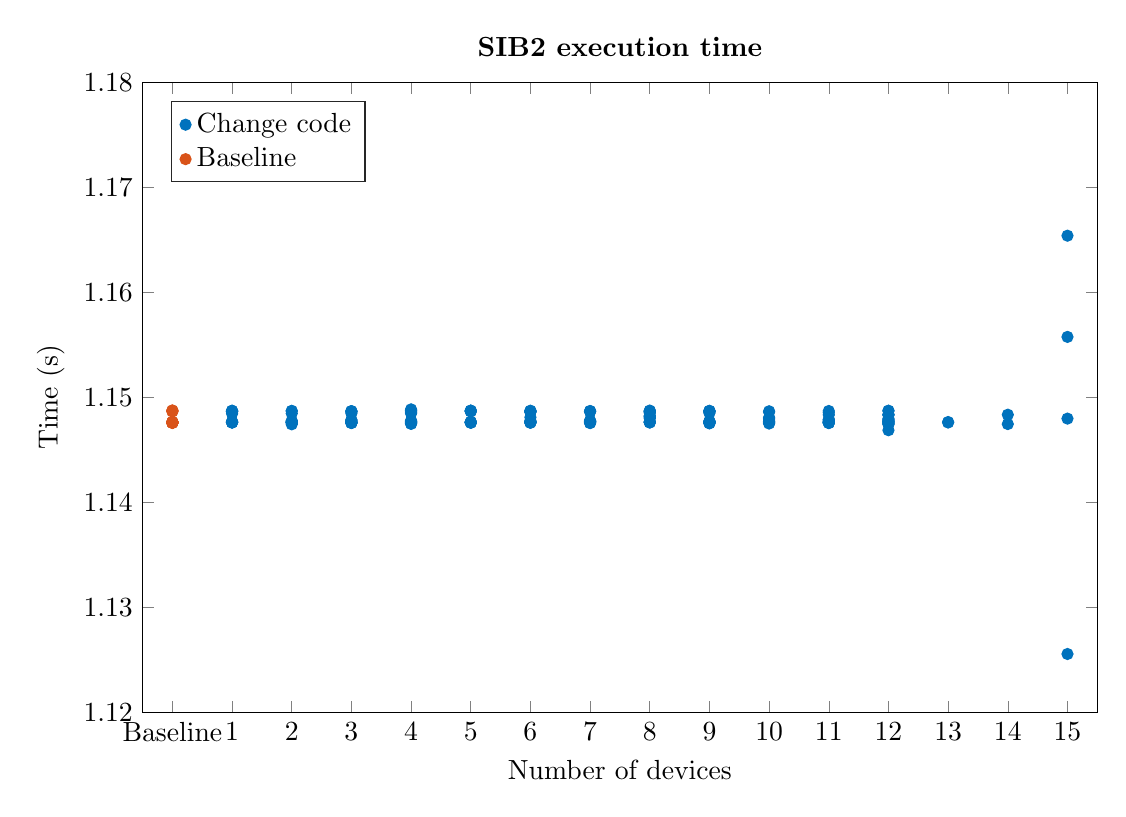
\begin{tikzpicture}

\begin{axis}[%
width=\textwidth,
height=.66\textwidth,
at={(0.758in,0.481in)},
scale only axis,
xmin=-0.5,
xmax=15.5,
xtick={0,1,2,3,4,5,6,7,8,9,10,11,12,13,14,15},
xticklabels={{Baseline},{1},{2},{3},{4},{5},{6},{7},{8},{9},{10},{11},{12},{13},{14},{15}},
xlabel={Number of devices},
ymin=1.12,
ymax=1.18,
ylabel={Time (s)},
axis background/.style={fill=white},
title style={font=\bfseries},
title={SIB2 execution time},
legend style={at={(0.03,0.97)},anchor=north west,legend cell align=left,align=left,draw=white!15!black}
]
\addplot [color=mycolor1,only marks,mark=*,mark options={solid}]
  table[row sep=crcr]{%
1	1.14861416816711\\
1	1.14764595031738\\
1	1.14869999885559\\
1	1.14867520332336\\
1	1.14768314361572\\
1	1.14871907234192\\
1	1.14760398864746\\
1	0\\
1	1.14761400222778\\
1	0\\
1	0\\
1	1.14873504638672\\
1	1.14866995811462\\
1	1.14762902259827\\
1	1.14844989776611\\
1	1.14772701263428\\
1	1.14866614341736\\
1	1.14762902259827\\
1	1.14766502380371\\
1	0\\
};
\addlegendentry{Change code};

\addplot [color=mycolor1,only marks,mark=*,mark options={solid},forget plot]
  table[row sep=crcr]{%
2	0\\
2	1.14869999885559\\
2	1.14872193336487\\
2	1.14743685722351\\
2	1.14759993553162\\
2	1.1476469039917\\
2	0\\
2	0\\
2	1.14758086204529\\
2	1.14762592315674\\
2	1.14773392677307\\
2	0\\
2	0\\
2	0\\
2	1.14763808250427\\
2	0\\
2	1.14763689041138\\
2	1.14846801757813\\
2	1.14778089523315\\
2	0\\
};

\addplot [color=mycolor1,only marks,mark=*,mark options={solid},forget plot]
  table[row sep=crcr]{%
3	0\\
3	1.1484739780426\\
3	1.14770102500916\\
3	1.14761209487915\\
3	1.14775395393372\\
3	1.14868903160095\\
3	0\\
3	1.14869093894959\\
3	1.14865207672119\\
3	1.14784407615662\\
3	1.14785313606262\\
3	1.14755582809448\\
3	0\\
3	1.14864993095398\\
3	0\\
3	0\\
3	1.14760112762451\\
3	1.14760613441467\\
3	1.14757800102234\\
3	1.14759707450867\\
};
\addplot [color=mycolor1,only marks,mark=*,mark options={solid},forget plot]
  table[row sep=crcr]{%
4	1.14768004417419\\
4	1.14766192436218\\
4	1.1485378742218\\
4	0\\
4	0\\
4	1.14876699447632\\
4	1.14763498306274\\
4	1.14748001098633\\
4	1.14754796028137\\
4	0\\
4	1.14770913124084\\
4	1.14860796928406\\
4	1.14766693115234\\
4	1.14847683906555\\
4	1.14886403083801\\
4	1.14751315116882\\
4	1.14781403541565\\
4	1.14758896827698\\
4	1.14863586425781\\
4	1.14876008033752\\
};
\addplot [color=mycolor1,only marks,mark=*,mark options={solid},forget plot]
  table[row sep=crcr]{%
5	1.14869904518127\\
5	1.14763689041138\\
5	1.14762902259827\\
5	1.14758992195129\\
5	1.14868807792664\\
5	0\\
5	0\\
5	1.14759087562561\\
5	1.14765095710754\\
5	0\\
5	0\\
5	1.14874196052551\\
5	1.14760994911194\\
5	1.14874196052551\\
5	0\\
5	0\\
5	0\\
5	0\\
5	1.1476788520813\\
5	1.14865398406982\\
};
\addplot [color=mycolor1,only marks,mark=*,mark options={solid},forget plot]
  table[row sep=crcr]{%
6	1.14870095252991\\
6	1.14779305458069\\
6	1.14860796928406\\
6	1.14767384529114\\
6	1.14760899543762\\
6	1.14768695831299\\
6	0\\
6	1.14863681793213\\
6	1.14810705184937\\
6	1.1475830078125\\
6	1.14868903160095\\
6	0\\
6	1.14762282371521\\
6	1.1486439704895\\
6	0\\
6	1.14873480796814\\
6	0\\
6	0\\
6	1.14763402938843\\
6	1.14762711524963\\
};
\addplot [color=mycolor1,only marks,mark=*,mark options={solid},forget plot]
  table[row sep=crcr]{%
7	1.14771604537964\\
7	0\\
7	1.14766097068787\\
7	1.14756989479065\\
7	0\\
7	1.14763617515564\\
7	1.1486930847168\\
7	0\\
7	0\\
7	0\\
7	1.14779114723206\\
7	1.14769601821899\\
7	1.14865589141846\\
7	1.14863991737366\\
7	1.14755702018738\\
7	1.1476879119873\\
7	0\\
7	1.14870691299438\\
7	1.14779496192932\\
7	1.14769411087036\\
};
\addplot [color=mycolor1,only marks,mark=*,mark options={solid},forget plot]
  table[row sep=crcr]{%
8	1.14765310287476\\
8	1.14868092536926\\
8	1.148521900177\\
8	1.14763808250427\\
8	0\\
8	1.14762806892395\\
8	1.14874792098999\\
8	0\\
8	1.14770197868347\\
8	1.14808297157288\\
8	0\\
8	1.14866805076599\\
8	0\\
8	1.14819407463074\\
8	1.14826083183289\\
8	1.14760708808899\\
8	1.14861392974854\\
8	1.1487021446228\\
8	1.14819502830505\\
8	1.14798307418823\\
};
\addplot [color=mycolor1,only marks,mark=*,mark options={solid},forget plot]
  table[row sep=crcr]{%
9	0\\
9	1.14850616455078\\
9	1.14752793312073\\
9	1.14864087104797\\
9	1.14869999885559\\
9	0\\
9	1.14872694015503\\
9	1.14868307113647\\
9	1.14765501022339\\
9	1.14763712882996\\
9	1.14769601821899\\
9	1.14774680137634\\
9	0\\
9	1.14756488800049\\
9	1.14765596389771\\
9	1.14865112304688\\
9	1.14868903160095\\
9	1.14756202697754\\
9	1.14766097068787\\
9	1.14769601821899\\
};
\addplot [color=mycolor1,only marks,mark=*,mark options={solid},forget plot]
  table[row sep=crcr]{%
10	0\\
10	1.14868307113647\\
10	1.14751195907593\\
10	1.14756798744202\\
10	0\\
10	0\\
10	0\\
10	1.14770293235779\\
10	0\\
10	0\\
10	1.14860892295837\\
10	1.1476309299469\\
10	1.14767909049988\\
10	0\\
10	0\\
10	1.14785599708557\\
10	1.14808678627014\\
10	1.1480119228363\\
10	0\\
10	0\\
};
\addplot [color=mycolor1,only marks,mark=*,mark options={solid},forget plot]
  table[row sep=crcr]{%
11	1.1487090587616\\
11	1.14756202697754\\
11	1.14763712882996\\
11	1.14790201187134\\
11	0\\
11	1.14756107330322\\
11	1.14760112762451\\
11	1.14776301383972\\
11	1.14790391921997\\
11	1.14773893356323\\
11	1.14760589599609\\
11	1.14763593673706\\
11	0\\
11	0\\
11	1.14833998680115\\
11	0\\
11	0\\
11	0\\
11	1.14766192436218\\
11	1.1485481262207\\
};
\addplot [color=mycolor1,only marks,mark=*,mark options={solid},forget plot]
  table[row sep=crcr]{%
12	1.147705078125\\
12	1.14687490463257\\
12	1.14872598648071\\
12	1.14797592163086\\
12	1.14834499359131\\
12	1.14762115478516\\
12	1.14752197265625\\
12	0\\
12	0\\
12	0\\
12	1.14772891998291\\
12	1.14748311042786\\
12	1.14785885810852\\
12	0\\
12	1.14766788482666\\
12	1.14836406707764\\
12	1.1478488445282\\
12	1.14873003959656\\
12	1.14742994308472\\
12	1.14833402633667\\
};
\addplot [color=mycolor1,only marks,mark=*,mark options={solid},forget plot]
  table[row sep=crcr]{%
13	0\\
13	0\\
13	0\\
13	0\\
13	1.14760804176331\\
13	0\\
13	0\\
13	0\\
13	0\\
13	0\\
13	0\\
13	0\\
13	0\\
13	0\\
13	1.1476571559906\\
13	0\\
13	0\\
13	0\\
13	0\\
13	0\\
};
\addplot [color=mycolor1,only marks,mark=*,mark options={solid},forget plot]
  table[row sep=crcr]{%
14	0\\
14	0\\
14	0\\
14	0\\
14	0\\
14	0\\
14	0\\
14	1.14835405349731\\
14	0\\
14	0\\
14	1.14746284484863\\
14	0\\
14	0\\
14	0\\
14	0\\
14	0\\
14	0\\
14	0\\
14	0\\
14	0\\
};
\addplot [color=mycolor1,only marks,mark=*,mark options={solid},forget plot]
  table[row sep=crcr]{%
15	1.12556910514832\\
15	0\\
15	0\\
15	1.14798092842102\\
15	0\\
15	1.15576195716858\\
15	0\\
15	0\\
15	0\\
15	0\\
15	0\\
15	0\\
15	1.16539812088013\\
15	0\\
15	0\\
15	0\\
15	0\\
15	0\\
15	0\\
15	0\\
};
\addplot [color=mycolor2,only marks,mark=*,mark options={solid}]
  table[row sep=crcr]{%
0	1.14874005317688\\
0	0\\
0	1.1475682258606\\
0	1.14761090278625\\
0	1.14760684967041\\
0	1.14865493774414\\
0	1.14760994911194\\
0	0\\
0	1.14760112762451\\
0	1.14764499664307\\
0	1.14870381355286\\
0	1.14764499664307\\
0	1.1476149559021\\
0	1.14760780334473\\
0	1.14760398864746\\
0	1.14765095710754\\
0	1.14761114120483\\
0	1.14876103401184\\
0	1.14763188362122\\
0	1.14761209487915\\
};
\addlegendentry{Baseline};

\end{axis}
\end{tikzpicture}%
\caption{Execution time for the decoding the NB-SIB2 step for different number of devices and the baseline emulator.}
\label{fig:MT_SIB2_Time}
\end{figure}


As seen on \autoref{fig:MT_SIB2_Time}, the baseline emulator and MDE have the same tendency, beside for when there is emulated 15 devices. There is not a big spread for the measurements of 1 through 14 devices, which is also expected as the timing between decoding NB-SIB1 and NB-SIB2 should only be the time until the whole NB-SIB2 have been received, with a small additional time for the decoding. 
\todo{explain why 15 is weird}


\subsection{NPRACH}
The execution time for the NPRACH step is measured from the decoding of NB-SIB2 is done until the msg1 is delivered to the transmit buffer, which gives the results seen on \autoref{fig:MT_Nprach_Time}. The NPRACH error occurs only when the MDE emulates more than 12 devices with a single exception. The NPRACH error happens, when only some of the devices get through the NPRACH step. As before the shown results are only for one of the emulated devices and the sample pool is not reduced by this error.
\todo{mads bør læse det her igen}

\begin{figure}[H]
\tikzsetnextfilename{MT_Nprach_Time}
\centering
\resizebox{0.5\textwidth}{!}{
% This file was created by matlab2tikz.
%
%The latest updates can be retrieved from
%  http://www.mathworks.com/matlabcentral/fileexchange/22022-matlab2tikz-matlab2tikz
%where you can also make suggestions and rate matlab2tikz.
%
\definecolor{mycolor1}{rgb}{0.00000,0.44700,0.74100}%
\definecolor{mycolor2}{rgb}{0.85000,0.32500,0.09800}%
%
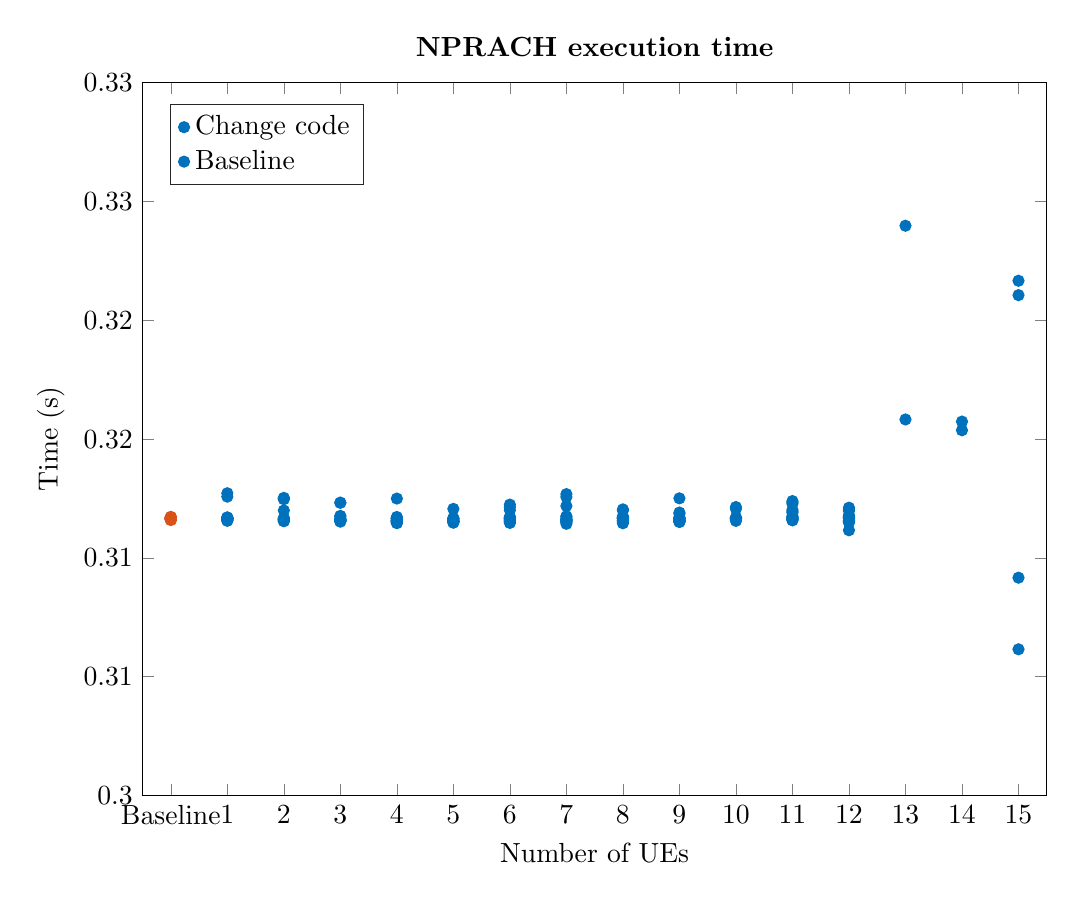
\begin{tikzpicture}

\begin{axis}[%
width=4.521in,
height=3.566in,
at={(0.758in,0.481in)},
scale only axis,
xmin=-0.5,
xmax=15.5,
xtick={0,1,2,3,4,5,6,7,8,9,10,11,12,13,14,15},
xticklabels={{Baseline},{1},{2},{3},{4},{5},{6},{7},{8},{9},{10},{11},{12},{13},{14},{15}},
xlabel={Number of UEs},
ymin=0.3,
ymax=0.33,
ylabel={Time (s)},
axis background/.style={fill=white},
title style={font=\bfseries},
title={NPRACH execution time},
legend style={at={(0.03,0.97)},anchor=north west,legend cell align=left,align=left,draw=white!15!black}
]
\addplot [color=mycolor1,only marks,mark=*,mark options={solid}]
  table[row sep=crcr]{%
1	0.311680793762207\\
1	0.311604022979736\\
1	0.311627864837646\\
1	0.311679840087891\\
1	0.311601877212524\\
1	0.311666011810303\\
1	0.311678886413574\\
1	0\\
1	0.311702966690063\\
1	0\\
1	0\\
1	0.311586856842041\\
1	0.311655044555664\\
1	0.311685085296631\\
1	0.311557054519653\\
1	0.312576055526733\\
1	0.311637878417969\\
1	0.312717914581299\\
1	0.311601161956787\\
1	0\\
};
\addlegendentry{Change code};

\addplot [color=mycolor1,only marks,mark=*,mark options={solid}]
  table[row sep=crcr]{%
2	0\\
2	0.311550140380859\\
2	0.311643123626709\\
2	0.31199312210083\\
2	0.311596870422363\\
2	0.31159496307373\\
2	0\\
2	0\\
2	0.311676025390625\\
2	0.311542987823486\\
2	0.312494993209839\\
2	0\\
2	0\\
2	0\\
2	0.311656951904297\\
2	0\\
2	0.312523126602173\\
2	0.311601877212524\\
2	0.312467098236084\\
2	0\\
};
\addlegendentry{Baseline};

\addplot [color=mycolor1,only marks,mark=*,mark options={solid},forget plot]
  table[row sep=crcr]{%
3	0\\
3	0.311551809310913\\
3	0.311765193939209\\
3	0.311564922332764\\
3	0.311563014984131\\
3	0.311522006988525\\
3	0\\
3	0.311599016189575\\
3	0.311592102050781\\
3	0.312321901321411\\
3	0.312319040298462\\
3	0.311748027801514\\
3	0\\
3	0.311631202697754\\
3	0\\
3	0\\
3	0.31165599822998\\
3	0.311599969863892\\
3	0.311576128005981\\
3	0.311599969863892\\
};
\addplot [color=mycolor1,only marks,mark=*,mark options={solid},forget plot]
  table[row sep=crcr]{%
4	0.311563014984131\\
4	0.311460018157959\\
4	0.311659097671509\\
4	0\\
4	0\\
4	0.311501979827881\\
4	0.311540126800537\\
4	0.311670064926147\\
4	0.31163501739502\\
4	0\\
4	0.311506986618042\\
4	0.311635971069336\\
4	0.31148099899292\\
4	0.311570167541504\\
4	0.311554193496704\\
4	0.311676979064941\\
4	0.312494039535522\\
4	0.311719179153442\\
4	0.311642169952393\\
4	0.311550855636597\\
};
\addplot [color=mycolor1,only marks,mark=*,mark options={solid},forget plot]
  table[row sep=crcr]{%
5	0.311535835266113\\
5	0.311478137969971\\
5	0.312060117721558\\
5	0.311666011810303\\
5	0.311637878417969\\
5	0\\
5	0\\
5	0.311530113220215\\
5	0.311499834060669\\
5	0\\
5	0\\
5	0.31154990196228\\
5	0.311671018600464\\
5	0.311539888381958\\
5	0\\
5	0\\
5	0\\
5	0\\
5	0.311614990234375\\
5	0.311556816101074\\
};
\addplot [color=mycolor1,only marks,mark=*,mark options={solid},forget plot]
  table[row sep=crcr]{%
6	0.311546087265015\\
6	0.311470031738281\\
6	0.311733961105347\\
6	0.311630010604858\\
6	0.312007188796997\\
6	0.311566114425659\\
6	0\\
6	0.311662197113037\\
6	0.31212592124939\\
6	0.3122398853302\\
6	0.311693906784058\\
6	0\\
6	0.311550140380859\\
6	0.311647891998291\\
6	0\\
6	0.311639070510864\\
6	0\\
6	0\\
6	0.311668872833252\\
6	0.311506032943726\\
};
\addplot [color=mycolor1,only marks,mark=*,mark options={solid},forget plot]
  table[row sep=crcr]{%
7	0.312558889389038\\
7	0\\
7	0.311611890792847\\
7	0.311638116836548\\
7	0\\
7	0.311750888824463\\
7	0.31158185005188\\
7	0\\
7	0\\
7	0\\
7	0.311608791351318\\
7	0.311516046524048\\
7	0.31172513961792\\
7	0.311556100845337\\
7	0.312680959701538\\
7	0.311551094055176\\
7	0\\
7	0.311511039733887\\
7	0.311432123184204\\
7	0.312183856964111\\
};
\addplot [color=mycolor1,only marks,mark=*,mark options={solid},forget plot]
  table[row sep=crcr]{%
8	0.311455965042114\\
8	0.311665058135986\\
8	0.311743974685669\\
8	0.311501026153564\\
8	0\\
8	0.311676025390625\\
8	0.311566114425659\\
8	0\\
8	0.311695098876953\\
8	0.311681032180786\\
8	0\\
8	0.311643838882446\\
8	0\\
8	0.312039852142334\\
8	0.31199312210083\\
8	0.311548948287964\\
8	0.311679840087891\\
8	0.311714887619019\\
8	0.31155800819397\\
8	0.311631917953491\\
};
\addplot [color=mycolor1,only marks,mark=*,mark options={solid},forget plot]
  table[row sep=crcr]{%
9	0\\
9	0.311545848846436\\
9	0.311694145202637\\
9	0.31157112121582\\
9	0.311569929122925\\
9	0\\
9	0.31165599822998\\
9	0.311696767807007\\
9	0.311599969863892\\
9	0.311621904373169\\
9	0.311509132385254\\
9	0.311530113220215\\
9	0\\
9	0.312504053115845\\
9	0.311852216720581\\
9	0.311555862426758\\
9	0.311640977859497\\
9	0.311907052993774\\
9	0.311527013778687\\
9	0.311538934707642\\
};
\addplot [color=mycolor1,only marks,mark=*,mark options={solid},forget plot]
  table[row sep=crcr]{%
10	0\\
10	0.311673879623413\\
10	0.311647891998291\\
10	0.311652898788452\\
10	0\\
10	0\\
10	0\\
10	0.311555862426758\\
10	0\\
10	0\\
10	0.31167197227478\\
10	0.312138080596924\\
10	0.31160306930542\\
10	0\\
10	0\\
10	0.312062978744507\\
10	0.311703205108643\\
10	0.311650991439819\\
10	0\\
10	0\\
};
\addplot [color=mycolor1,only marks,mark=*,mark options={solid},forget plot]
  table[row sep=crcr]{%
11	0.311681032180786\\
11	0.31174898147583\\
11	0.311945915222168\\
11	0.312388181686401\\
11	0\\
11	0.311898946762085\\
11	0.311634063720703\\
11	0.312273979187012\\
11	0.31233811378479\\
11	0.311637878417969\\
11	0.311670064926147\\
11	0.311576128005981\\
11	0\\
11	0\\
11	0.312019824981689\\
11	0\\
11	0\\
11	0\\
11	0.311609029769897\\
11	0.311727046966553\\
};
\addplot [color=mycolor1,only marks,mark=*,mark options={solid},forget plot]
  table[row sep=crcr]{%
12	0.311507940292358\\
12	0.311978101730347\\
12	0.311573028564453\\
12	0.311161041259766\\
12	0.312034130096436\\
12	0.311545848846436\\
12	0.311670064926147\\
12	0\\
12	0\\
12	0\\
12	0.311485052108765\\
12	0.311722993850708\\
12	0.311711072921753\\
12	0\\
12	0.31154990196228\\
12	0.311701059341431\\
12	0.31179404258728\\
12	0.311655044555664\\
12	0.311732053756714\\
12	0.312110900878906\\
};
\addplot [color=mycolor1,only marks,mark=*,mark options={solid},forget plot]
  table[row sep=crcr]{%
13	0\\
13	0\\
13	0\\
13	0\\
13	0.315821886062622\\
13	0\\
13	0\\
13	0\\
13	0\\
13	0\\
13	0\\
13	0\\
13	0\\
13	0\\
13	0.323969841003418\\
13	0\\
13	0\\
13	0\\
13	0\\
13	0\\
};
\addplot [color=mycolor1,only marks,mark=*,mark options={solid},forget plot]
  table[row sep=crcr]{%
14	0\\
14	0\\
14	0\\
14	0\\
14	0\\
14	0\\
14	0\\
14	0.315366983413696\\
14	0\\
14	0\\
14	0.315733194351196\\
14	0\\
14	0\\
14	0\\
14	0\\
14	0\\
14	0\\
14	0\\
14	0\\
14	0\\
};
\addplot [color=mycolor1,only marks,mark=*,mark options={solid},forget plot]
  table[row sep=crcr]{%
15	0.309165954589844\\
15	0\\
15	0\\
15	0.321655988693237\\
15	0\\
15	0.306154012680054\\
15	0\\
15	0\\
15	0\\
15	0\\
15	0\\
15	0\\
15	0.321050882339478\\
15	0\\
15	0\\
15	0\\
15	0\\
15	0\\
15	0\\
15	0\\
};
\addplot [color=mycolor2,only marks,mark=*,mark options={solid},forget plot]
  table[row sep=crcr]
\caption{Execution time for the NPRACH step for different number of devices and the baseline emulator.}
\label{fig:MT_Nprach_Time}
\end{figure}

As seen on \autoref{fig:MT_Nprach_Time} the baseline emulator and MDE takes approximately the same time, but the MDE has a bigger spread of its measurement points. All the measurements of the MDE with more than 12 devices, does not follow the tendency of the other measurements. This should come from the fact, that all the shown measurement points for these number of devices, is measurements where the NPRACH error occurred and none of them made it error free through, as seen on \autoref{fig:MT_error_dist}.

\subsection{RAR}
The execution time for the RAR step is measured from msg1 is delivered to the transmit buffer until msg2 is received, which gives the results seen on \autoref{fig:MT_Rar_Time}. The msg2 error occurs here, if no msg2 is received and the measurements are therefore excluded. 

\begin{figure}[H]
\tikzsetnextfilename{MT_Rar_Time}
\centering
\resizebox{0.5\textwidth}{!}{
% This file was created by matlab2tikz.
%
%The latest updates can be retrieved from
%  http://www.mathworks.com/matlabcentral/fileexchange/22022-matlab2tikz-matlab2tikz
%where you can also make suggestions and rate matlab2tikz.
%
\definecolor{mycolor1}{rgb}{0.00000,0.44700,0.74100}%
\definecolor{mycolor2}{rgb}{0.85000,0.32500,0.09800}%
%
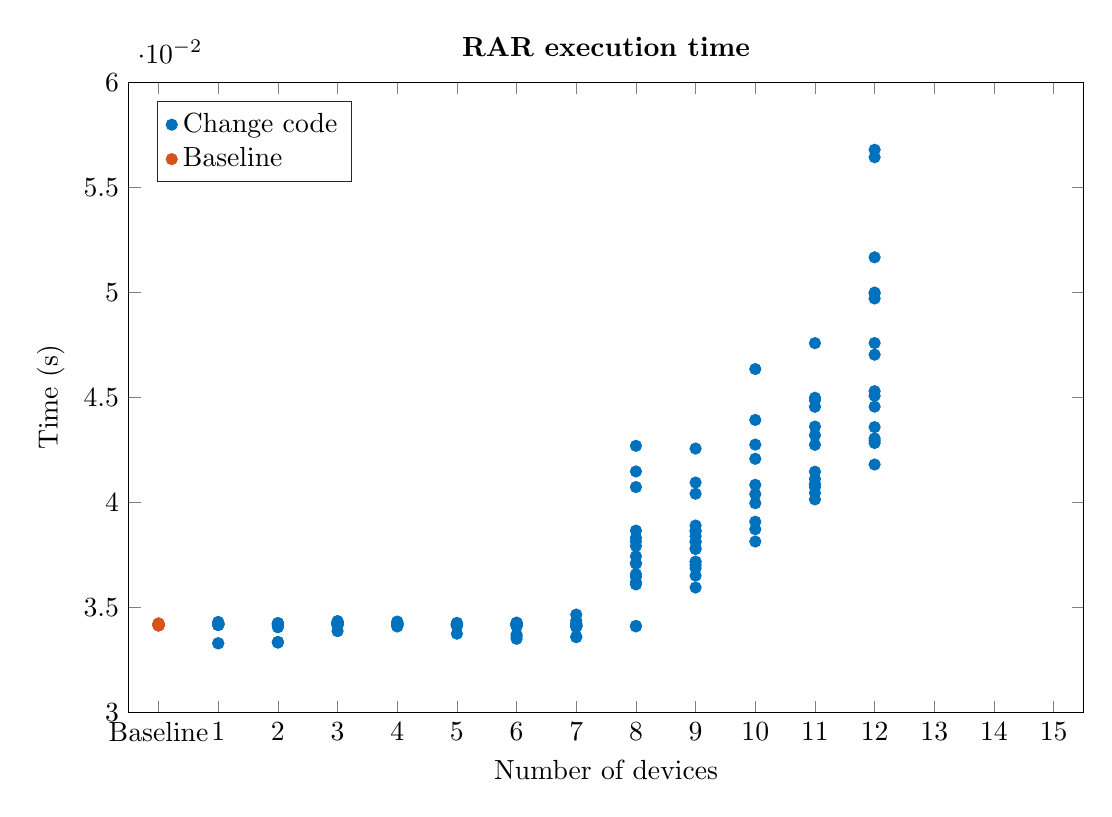
\begin{tikzpicture}

\begin{axis}[%
width=\textwidth,
height=.66\textwidth,
at={(0.758in,0.481in)},
scale only axis,
xmin=-0.5,
xmax=15.5,
xtick={0,1,2,3,4,5,6,7,8,9,10,11,12,13,14,15},
xticklabels={{Baseline},{1},{2},{3},{4},{5},{6},{7},{8},{9},{10},{11},{12},{13},{14},{15}},
xlabel={Number of devices},
ymin=0.03,
ymax=0.06,
ylabel={Time (s)},
axis background/.style={fill=white},
title style={font=\bfseries},
title={RAR execution time},
legend style={at={(0.03,0.97)},anchor=north west,legend cell align=left,align=left,draw=white!15!black}
]
\addplot [color=mycolor1,only marks,mark=*,mark options={solid}]
  table[row sep=crcr]{%
1	0.0341880321502686\\
1	0.034235954284668\\
1	0.0342159271240234\\
1	0.0342271327972412\\
1	0.0342719554901123\\
1	0.0341730117797852\\
1	0\\
1	0\\
1	0.0341699123382568\\
1	0\\
1	0\\
1	0.0342731475830078\\
1	0.0341849327087402\\
1	0.0341880321502686\\
1	0.0343189239501953\\
1	0.0333008766174316\\
1	0.0342051982879639\\
1	0.033297061920166\\
1	0.0342288017272949\\
1	0\\
};
\addlegendentry{Change code};

\addplot [color=mycolor1,only marks,mark=*,mark options={solid},forget plot]
  table[row sep=crcr]{%
2	0\\
2	0.0342118740081787\\
2	0.0341849327087402\\
2	0.0340640544891357\\
2	0.0342371463775635\\
2	0.0342140197753906\\
2	0\\
2	0\\
2	0.0341610908508301\\
2	0.0342671871185303\\
2	0.0333490371704102\\
2	0\\
2	0\\
2	0\\
2	0.0342299938201904\\
2	0\\
2	0.0333659648895264\\
2	0.0342400074005127\\
2	0.0333349704742432\\
2	0\\
};

\addplot [color=mycolor1,only marks,mark=*,mark options={solid},forget plot]
  table[row sep=crcr]{%
3	0\\
3	0.0342600345611572\\
3	0.0338799953460693\\
3	0.0342161655426025\\
3	0.0342400074005127\\
3	0.0343279838562012\\
3	0\\
3	0.0342199802398682\\
3	0.0342228412628174\\
3	0.0342550277709961\\
3	0.0343589782714844\\
3	0.0341391563415527\\
3	0\\
3	0.0343039035797119\\
3	0\\
3	0\\
3	0.0342159271240234\\
3	0.03420090675354\\
3	0.0342509746551514\\
3	0.0342059135437012\\
};
\addplot [color=mycolor1,only marks,mark=*,mark options={solid},forget plot]
  table[row sep=crcr]{%
4	0.0342638492584229\\
4	0.0343360900878906\\
4	0.0341908931732178\\
4	0\\
4	0\\
4	0.0342490673065186\\
4	0.0342738628387451\\
4	0.0342228412628174\\
4	0.0341949462890625\\
4	0\\
4	0.0342400074005127\\
4	0.0342440605163574\\
4	0.0342991352081299\\
4	0.0341489315032959\\
4	0.0341489315032959\\
4	0.0342459678649902\\
4	0.0341918468475342\\
4	0.0341000556945801\\
4	0.034153938293457\\
4	0.034203052520752\\
};
\addplot [color=mycolor1,only marks,mark=*,mark options={solid},forget plot]
  table[row sep=crcr]{%
5	0.0342710018157959\\
5	0.0341567993164063\\
5	0.0337579250335693\\
5	0.0341598987579346\\
5	0.0341479778289795\\
5	0\\
5	0\\
5	0.0342059135437012\\
5	0.0342340469360352\\
5	0\\
5	0\\
5	0.0342390537261963\\
5	0.0341389179229736\\
5	0.0341851711273193\\
5	0\\
5	0\\
5	0\\
5	0\\
5	0.034188985824585\\
5	0.0342321395874023\\
};
\addplot [color=mycolor1,only marks,mark=*,mark options={solid},forget plot]
  table[row sep=crcr]{%
6	0.0342798233032227\\
6	0.0341129302978516\\
6	0.0341250896453857\\
6	0.0342040061950684\\
6	0.0337188243865967\\
6	0.0342609882354736\\
6	0\\
6	0.0342237949371338\\
6	0.0336298942565918\\
6	0.0335140228271484\\
6	0.0341589450836182\\
6	0\\
6	0.0342769622802734\\
6	0.0342199802398682\\
6	0\\
6	0.0342271327972412\\
6	0\\
6	0\\
6	0.0341720581054688\\
6	0\\
};
\addplot [color=mycolor1,only marks,mark=*,mark options={solid},forget plot]
  table[row sep=crcr]{%
7	0.0336170196533203\\
7	0\\
7	0.0341181755065918\\
7	0.0341799259185791\\
7	0\\
7	0.0342490673065186\\
7	0.0342171192169189\\
7	0\\
7	0\\
7	0\\
7	0.0346660614013672\\
7	0.0343749523162842\\
7	0.0340960025787354\\
7	0.0341479778289795\\
7	0.0340781211853027\\
7	0.0341360569000244\\
7	0\\
7	0.0341110229492188\\
7	0.034153938293457\\
7	0.0335919857025146\\
};
\addplot [color=mycolor1,only marks,mark=*,mark options={solid},forget plot]
  table[row sep=crcr]{%
8	0.0365910530090332\\
8	0.0427010059356689\\
8	0.0370931625366211\\
8	0.0381538867950439\\
8	0\\
8	0.0364658832550049\\
8	0.0379340648651123\\
8	0\\
8	0.0374419689178467\\
8	0.0407381057739258\\
8	0\\
8	0.0341041088104248\\
8	0\\
8	0.0414822101593018\\
8	0.0361030101776123\\
8	0.0386650562286377\\
8	0.0383260250091553\\
8	0.0362110137939453\\
8	0.0341310501098633\\
8	0.037121057510376\\
};
\addplot [color=mycolor1,only marks,mark=*,mark options={solid},forget plot]
  table[row sep=crcr]{%
9	0\\
9	0.0370240211486816\\
9	0.0365219116210938\\
9	0.0378210544586182\\
9	0.038114070892334\\
9	0\\
9	0.037787914276123\\
9	0.0381491184234619\\
9	0.0389068126678467\\
9	0.0386679172515869\\
9	0.0383989810943604\\
9	0.0359559059143066\\
9	0\\
9	0.042572021484375\\
9	0.0371799468994141\\
9	0.0409531593322754\\
9	0.0386199951171875\\
9	0.0404210090637207\\
9	0.036876916885376\\
9	0.0371849536895752\\
};
\addplot [color=mycolor1,only marks,mark=*,mark options={solid},forget plot]
  table[row sep=crcr]{%
10	0\\
10	0.0420839786529541\\
10	0.0408451557159424\\
10	0.0439350605010986\\
10	0\\
10	0\\
10	0\\
10	0.0399701595306396\\
10	0\\
10	0\\
10	0.0381450653076172\\
10	0.0463569164276123\\
10	0.0390889644622803\\
10	0\\
10	0\\
10	0.0403990745544434\\
10	0.0427589416503906\\
10	0.0387308597564697\\
10	0\\
10	0\\
};
\addplot [color=mycolor1,only marks,mark=*,mark options={solid},forget plot]
  table[row sep=crcr]{%
11	0.0449898242950439\\
11	0.0432069301605225\\
11	0.0445609092712402\\
11	0.0408809185028076\\
11	0\\
11	0.0404579639434814\\
11	0.0427489280700684\\
11	0.0475912094116211\\
11	0.0448739528656006\\
11	0.0414700508117676\\
11	0.0436179637908936\\
11	0.0411219596862793\\
11	0\\
11	0\\
11	0.0407330989837646\\
11	0\\
11	0\\
11	0\\
11	0.0408778190612793\\
11	0.040151834487915\\
};
\addplot [color=mycolor1,only marks,mark=*,mark options={solid},forget plot]
  table[row sep=crcr]{%
12	0.0453028678894043\\
12	0.0516760349273682\\
12	0.0564429759979248\\
12	0.0475959777832031\\
12	0.0430538654327393\\
12	0.0450849533081055\\
12	0.0470409393310547\\
12	0\\
12	0\\
12	0\\
12	0.0429530143737793\\
12	0.0567960739135742\\
12	0.0497169494628906\\
12	0\\
12	0.0499541759490967\\
12	0.0428369045257568\\
12	0.0435919761657715\\
12	0.0445668697357178\\
12	0.0499989986419678\\
12	0.0418119430541992\\
};
\addplot [color=mycolor1,only marks,mark=*,mark options={solid},forget plot]
  table[row sep=crcr]{%
13	0\\
13	0\\
13	0\\
13	0\\
13	0\\
13	0\\
13	0\\
13	0\\
13	0\\
13	0\\
13	0\\
13	0\\
13	0\\
13	0\\
13	0\\
13	0\\
13	0\\
13	0\\
13	0\\
13	0\\
};
\addplot [color=mycolor1,only marks,mark=*,mark options={solid},forget plot]
  table[row sep=crcr]{%
14	0\\
14	0\\
14	0\\
14	0\\
14	0\\
14	0\\
14	0\\
14	0\\
14	0\\
14	0\\
14	0\\
14	0\\
14	0\\
14	0\\
14	0\\
14	0\\
14	0\\
14	0\\
14	0\\
14	0\\
};
\addplot [color=mycolor1,only marks,mark=*,mark options={solid},forget plot]
  table[row sep=crcr]{%
15	0\\
15	0\\
15	0\\
15	0\\
15	0\\
15	0\\
15	0\\
15	0\\
15	0\\
15	0\\
15	0\\
15	0\\
15	0\\
15	0\\
15	0\\
15	0\\
15	0\\
15	0\\
15	0\\
15	0\\
};
\addplot [color=mycolor2,only marks,mark=*,mark options={solid}]
  table[row sep=crcr]
\caption{Execution time for the decoding the MIB-NB for different number of devices and the baseline emulator. A single measurement for the baseline is placed at 5.0834 s, which is not shown on this figure.}
\label{fig:MT_Rar_Time}
\end{figure}

As seen on \autoref{fig:MT_Rar_Time} the MDE starts out following the tendency of the baseline emulator, but around eight devices it begins to get a higher and higher execution time and getting a wider spread compared to the values at a low number of devices, which indicates a possible bottleneck in the system.

\subsection{Summary}
When looking at the execution time, of the MDE compared to the baseline emulator, it can be seen that in most steps, the two emulators perform similarly. The initialization steps is where the biggest difference is, but as the extra is performed in a single thread, this is to be expected. This is however not a problem as the real time dependency of the system has not yet been invoked. A bottleneck that can be seen in these test, comes in the RAR step, where an increase in delay is seen, when the number of number of devices gets above eight. The results from 13 to 15 device do act as the other measurements, but with no successful runs, is this expected as well. \todo{what do you mean, with the last part}


\section{CPU usage}
To test the CPU usage of the MDE, the test is split up into different steps as discussed in \autoref{sub:MassStruct}. 

The results is shown as average CPU usage over the steps time period, as the executing time is not equal for all measurement. The errors mentioned thorughout \autoref{sec:exeTime} is also effecting the CPU measurements and the measurement points, which have an error is removed from the sample pool for all consecutive steps.

The sample rate is 3 Hz, this is a rather slow sample rate, compared to the execution time for the different steps. This is the highest sample rate of any tool tested. The time window for the RAR step is unfortunately too small to be measured with a 3 Hz sample rate. The tool can not distinguish between individual cores of the PC and adds the usage together. In \appref{app:PC_stat} the number of cores in the PC is shown to be 8. A conservative estimation is made, that only 7 of these is available for the MDE, with the final 1 running background programs on the PC. 

\subsection{Initialization}
The initialization step is measured from the start of the emulator to the cell search begin. The average CPU usage of the MDE and baseline emulator can be seen on \autoref{fig:CPU_init}.

\begin{figure}[H]
\tikzsetnextfilename{CPU_init}
\centering
\resizebox{0.5\textwidth}{!}{
% This file was created by matlab2tikz.
%
%The latest updates can be retrieved from
%  http://www.mathworks.com/matlabcentral/fileexchange/22022-matlab2tikz-matlab2tikz
%where you can also make suggestions and rate matlab2tikz.
%
\definecolor{mycolor1}{rgb}{0.00000,0.44700,0.74100}%
\definecolor{mycolor2}{rgb}{0.85000,0.32500,0.09800}%
%
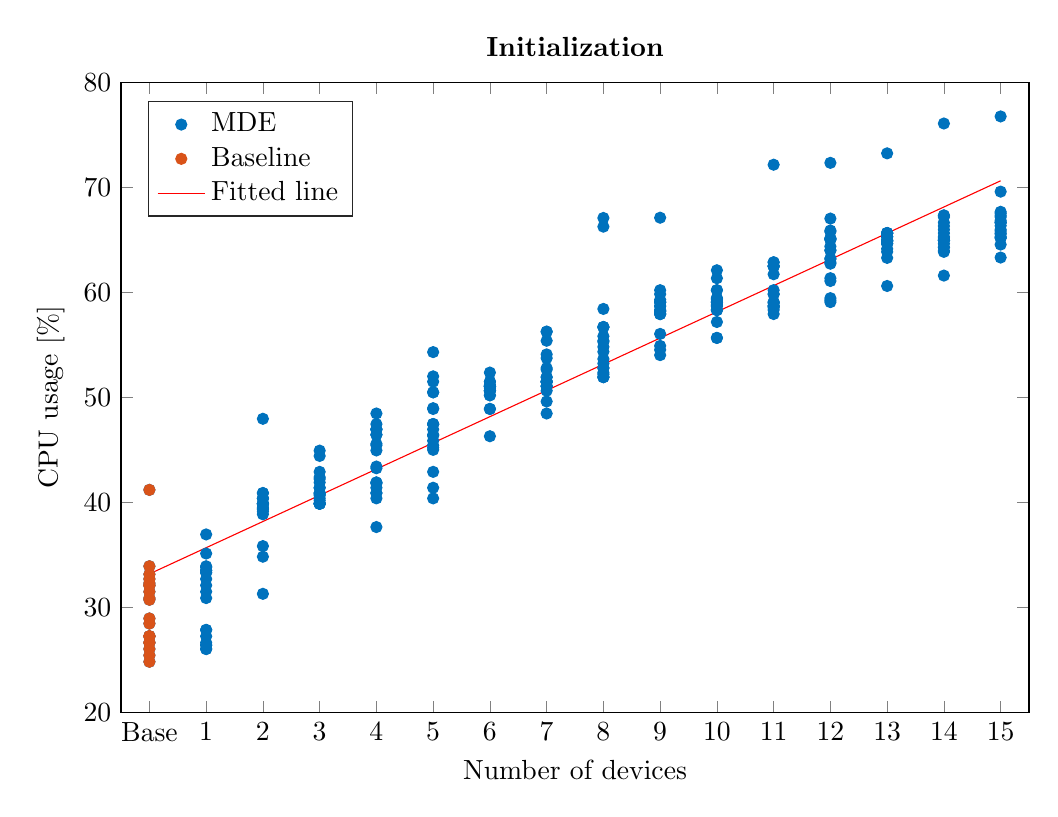
\begin{tikzpicture}

\begin{axis}[%
width=0.951\textwidth,
height=0.66\textwidth,
at={(0\textwidth,0\textwidth)},
scale only axis,
xmin=-0.5,
xmax=15.5,
xtick={0,1,2,3,4,5,6,7,8,9,10,11,12,13,14,15},
xticklabels={{Base},{1},{2},{3},{4},{5},{6},{7},{8},{9},{10},{11},{12},{13},{14},{15}},
xlabel={Number of devices},
ymin=20,
ymax=80,
ylabel={CPU usage [\%]},
axis background/.style={fill=white},
title style={font=\bfseries},
title={Initialization},
legend style={at={(0.03,0.97)},anchor=north west,legend cell align=left,align=left,draw=white!15!black},
y tick label style={/pgf/number format/fixed}
]
\addplot [color=mycolor1,only marks,mark=*,mark options={solid}]
  table[row sep=crcr]{%
0	32.12\\
1	35.15\\
2	39.5416666666667\\
3	40.9083333333333\\
4	37.67\\
5	48.9883333333333\\
6	51.0814285714286\\
7	49.6285714285714\\
8	55.8428571428571\\
9	58.18875\\
10	59.08875\\
11	58.71125\\
12	65.15\\
13	65.6566666666667\\
14	64.9822222222222\\
15	67.5488888888889\\
0	24.848\\
1	26.058\\
2	39.8983333333333\\
3	40.195\\
4	41.815\\
5	46.36\\
6	51.0828571428572\\
7	53.7571428571429\\
8	67.1\\
9	60.225\\
10	58.3325\\
11	62.51125\\
12	65.1725\\
13	65.3188888888889\\
14	65.3188888888889\\
15	65.8544444444444\\
0	41.21\\
1	26.434\\
2	40.9066666666667\\
3	41.9166666666667\\
4	46.465\\
5	48.9157142857143\\
6	48.9157142857143\\
7	52.8114285714286\\
8	56.7085714285714\\
9	59.3125\\
10	59.46875\\
11	62.87875\\
12	65.9075\\
13	60.6244444444444\\
14	64.9822222222222\\
15	65.6544444444444\\
0	28.484\\
1	26.416\\
2	40.9066666666667\\
3	42.9266666666667\\
4	46.9683333333333\\
5	40.4016666666667\\
6	51.5142857142857\\
7	51.0814285714286\\
8	51.9457142857143\\
9	56.06\\
10	59.08875\\
11	59.09\\
12	61.1\\
13	64.9811111111111\\
14	66.6666666666667\\
15	66.363\\
0	27.27\\
1	33.562\\
2	39.8966666666667\\
3	39.8966666666667\\
4	40.9066666666667\\
5	54.3285714285714\\
6	50.6485714285714\\
7	51.08\\
8	51.9457142857143\\
9	59.84625\\
10	60.225\\
11	57.95375\\
12	65.05\\
13	64.6455555555555\\
14	66.33\\
15	65.17\\
0	30.748\\
1	32.726\\
2	35.8566666666667\\
3	41.4116666666667\\
4	41.4116666666667\\
5	45.4533333333333\\
6	50.9157142857143\\
7	48.4828571428571\\
8	66.2728571428571\\
9	57.95375\\
10	59.09125\\
11	58.99\\
12	72.34875\\
13	64.6444444444444\\
14	67.34\\
15	76.7688888888889\\
0	33.172\\
1	26.058\\
2	34.8466666666667\\
3	40.67\\
4	46.9683333333333\\
5	46.9683333333333\\
6	50.6471428571429\\
7	51.5128571428571\\
8	52.8128571428571\\
9	57.95375\\
10	60.225\\
11	61.7425\\
12	67.04375\\
13	64.8744444444445\\
14	65.6555555555556\\
15	65.3177777777778\\
0	26.058\\
1	33.3316666666667\\
2	47.9783333333333\\
3	39.8983333333333\\
4	40.9066666666667\\
5	45.02\\
6	50.2157142857143\\
7	51.9457142857143\\
8	55.41\\
9	58.33125\\
10	59.32375\\
11	59.8475\\
12	65.79625\\
13	65.3188888888889\\
14	64.9811111111111\\
15	65.24\\
0	32.334\\
1	31.514\\
2	39.8233333333333\\
3	44.4416666666667\\
4	43.2683333333333\\
5	42.9266666666667\\
6	50.6471428571429\\
7	51.0814285714286\\
8	52.3785714285714\\
9	58.71125\\
10	58.7225\\
11	58.3425\\
12	64.01375\\
13	64.9822222222222\\
14	67.34\\
15	67.34\\
0	31.514\\
1	26.664\\
2	31.3116666666667\\
3	42.4216666666667\\
4	45.6016666666667\\
5	50.5033333333333\\
6	51.0814285714286\\
7	50.6471428571429\\
8	55.30125\\
9	58.19875\\
10	59.4675\\
11	58.56625\\
12	59.4675\\
13	63.8733333333333\\
14	64.6466666666667\\
15	65.9933333333333\\
0	32.726\\
1	33.332\\
2	40.4016666666667\\
3	42.2433333333333\\
4	48.4833333333333\\
5	46.4633333333333\\
6	50.2142857142857\\
7	51.5142857142857\\
8	56.7214285714286\\
9	58.71\\
10	58.71\\
11	59.09\\
12	59.2588888888889\\
13	65.6566666666667\\
14	67.1911111111111\\
15	69.6066666666667\\
0	30.908\\
1	36.968\\
2	40.4016666666667\\
3	39.8983333333333\\
4	40.4033333333333\\
5	47.4733333333333\\
6	52.38\\
7	56.2757142857143\\
8	52.8114285714286\\
9	59.09\\
10	62.12125\\
11	60.22625\\
12	63.17875\\
13	65.6566666666667\\
14	61.6144444444444\\
15	63.333\\
0	27.27\\
1	27.876\\
2	40.4016666666667\\
3	39.8966666666667\\
4	41.9166666666667\\
5	50.4942857142857\\
6	51.0814285714286\\
7	51.9457142857143\\
8	53.2442857142857\\
9	54.9225\\
10	58.3325\\
11	72.17125\\
12	62.745\\
13	65.3188888888889\\
14	64.3077777777778\\
15	64.5666666666667\\
0	27.27\\
1	27.876\\
2	39.3916666666667\\
3	39.8966666666667\\
4	44.965\\
5	45.2166666666667\\
6	50.6485714285714\\
7	51.5128571428572\\
8	53.6771428571429\\
9	54.0425\\
10	55.68125\\
11	62.49875\\
12	62.87875\\
13	63.2988888888889\\
14	63.9711111111111\\
15	67.6866666666667\\
0	32.104\\
1	33.938\\
2	38.8866666666667\\
3	40.7883333333333\\
4	45.455\\
5	41.4116666666667\\
6	51.5142857142857\\
7	54.11\\
8	52.2142857142857\\
9	67.125\\
10	58.33125\\
11	58.71\\
12	65.03875\\
13	64.8333333333333\\
14	65.2\\
15	66.8655555555556\\
0	26.664\\
1	33.528\\
2	39.155\\
3	39.8966666666667\\
4	46.4633333333333\\
5	47.4733333333333\\
6	46.3185714285714\\
7	51.5128571428571\\
8	54.3657142857143\\
9	57.9525\\
10	58.855\\
11	62.87875\\
12	64.01625\\
13	65.6566666666667\\
14	76.0944444444444\\
15	66.6655555555555\\
0	26.664\\
1	27.27\\
2	39.3916666666667\\
3	40.4033333333333\\
4	43.4316666666667\\
5	52.0183333333333\\
6	48.9171428571429\\
7	55.41\\
8	51.9457142857143\\
9	59.09\\
10	55.68\\
11	62.49875\\
12	61.3677777777778\\
13	64.9811111111111\\
14	64.9822222222222\\
15	65.5666666666667\\
0	25.452\\
1	32.12\\
2	39.8966666666667\\
3	40.9083333333333\\
4	46.9683333333333\\
5	51.5133333333333\\
6	51.1971428571429\\
7	52.6585714285714\\
8	58.44\\
9	59.09\\
10	57.195\\
11	59.84625\\
12	59.08875\\
13	64.16\\
14	65.9922222222222\\
15	66.6666666666667\\
0	33.938\\
1	33.8383333333333\\
2	39.8983333333333\\
3	41.4116666666667\\
4	47.4733333333333\\
5	45.8857142857143\\
6	51.08\\
7	51.5128571428572\\
8	54.8242857142857\\
9	54.54375\\
10	59.09\\
11	58.71\\
12	63.25625\\
13	73.2533333333333\\
14	64.3088888888889\\
15	66.666\\
0	28.966\\
1	30.908\\
2	39.8983333333333\\
3	44.9483333333333\\
4	41.9166666666667\\
5	47.4733333333333\\
6	51.08\\
7	56.2757142857143\\
8	56.7085714285714\\
9	58.31\\
10	61.3625\\
11	62.5\\
12	64.3925\\
13	65.6566666666667\\
14	63.8733333333333\\
15	67.1922222222222\\
};
\addlegendentry{MDE};

\addplot [color=mycolor2,only marks,mark=*,mark options={solid}]
  table[row sep=crcr]{%
0	32.12\\
0	24.848\\
0	41.21\\
0	28.484\\
0	27.27\\
0	30.748\\
0	33.172\\
0	26.058\\
0	32.334\\
0	31.514\\
0	32.726\\
0	30.908\\
0	27.27\\
0	27.27\\
0	32.104\\
0	26.664\\
0	26.664\\
0	25.452\\
0	33.938\\
0	28.966\\
};
\addlegendentry{Baseline};

\addplot [color=red,solid]
  table[row sep=crcr]{%
0	33.2067881900678\\
0.015	33.2442223433503\\
0.03	33.2816564966329\\
0.045	33.3190906499155\\
0.06	33.356524803198\\
0.075	33.3939589564806\\
0.09	33.4313931097632\\
0.105	33.4688272630457\\
0.12	33.5062614163283\\
0.135	33.5436955696108\\
0.15	33.5811297228934\\
0.165	33.618563876176\\
0.18	33.6559980294585\\
0.195	33.6934321827411\\
0.21	33.7308663360237\\
0.225	33.7683004893062\\
0.24	33.8057346425888\\
0.255	33.8431687958713\\
0.27	33.8806029491539\\
0.285	33.9180371024365\\
0.3	33.955471255719\\
0.315	33.9929054090016\\
0.33	34.0303395622842\\
0.345	34.0677737155667\\
0.36	34.1052078688493\\
0.375	34.1426420221318\\
0.39	34.1800761754144\\
0.405	34.217510328697\\
0.42	34.2549444819795\\
0.435	34.2923786352621\\
0.45	34.3298127885447\\
0.465	34.3672469418272\\
0.48	34.4046810951098\\
0.495	34.4421152483923\\
0.51	34.4795494016749\\
0.525	34.5169835549575\\
0.54	34.55441770824\\
0.555	34.5918518615226\\
0.57	34.6292860148052\\
0.585	34.6667201680877\\
0.6	34.7041543213703\\
0.615	34.7415884746529\\
0.63	34.7790226279354\\
0.645	34.816456781218\\
0.66	34.8538909345005\\
0.675	34.8913250877831\\
0.69	34.9287592410657\\
0.705	34.9661933943482\\
0.72	35.0036275476308\\
0.735	35.0410617009134\\
0.75	35.0784958541959\\
0.765	35.1159300074785\\
0.78	35.153364160761\\
0.795	35.1907983140436\\
0.81	35.2282324673262\\
0.825	35.2656666206087\\
0.84	35.3031007738913\\
0.855	35.3405349271739\\
0.87	35.3779690804564\\
0.885	35.415403233739\\
0.9	35.4528373870215\\
0.915	35.4902715403041\\
0.93	35.5277056935867\\
0.945	35.5651398468692\\
0.96	35.6025740001518\\
0.975	35.6400081534344\\
0.99	35.6774423067169\\
1.005	35.7148764599995\\
1.02	35.752310613282\\
1.035	35.7897447665646\\
1.05	35.8271789198472\\
1.065	35.8646130731297\\
1.08	35.9020472264123\\
1.095	35.9394813796949\\
1.11	35.9769155329774\\
1.125	36.01434968626\\
1.14	36.0517838395426\\
1.155	36.0892179928251\\
1.17	36.1266521461077\\
1.185	36.1640862993902\\
1.2	36.2015204526728\\
1.215	36.2389546059554\\
1.23	36.2763887592379\\
1.245	36.3138229125205\\
1.26	36.3512570658031\\
1.275	36.3886912190856\\
1.29	36.4261253723682\\
1.305	36.4635595256507\\
1.32	36.5009936789333\\
1.335	36.5384278322159\\
1.35	36.5758619854984\\
1.365	36.613296138781\\
1.38	36.6507302920636\\
1.395	36.6881644453461\\
1.41	36.7255985986287\\
1.425	36.7630327519112\\
1.44	36.8004669051938\\
1.455	36.8379010584764\\
1.47	36.8753352117589\\
1.485	36.9127693650415\\
1.5	36.9502035183241\\
1.515	36.9876376716066\\
1.53	37.0250718248892\\
1.545	37.0625059781718\\
1.56	37.0999401314543\\
1.575	37.1373742847369\\
1.59	37.1748084380194\\
1.605	37.212242591302\\
1.62	37.2496767445846\\
1.635	37.2871108978671\\
1.65	37.3245450511497\\
1.665	37.3619792044323\\
1.68	37.3994133577148\\
1.695	37.4368475109974\\
1.71	37.4742816642799\\
1.725	37.5117158175625\\
1.74	37.5491499708451\\
1.755	37.5865841241276\\
1.77	37.6240182774102\\
1.785	37.6614524306928\\
1.8	37.6988865839753\\
1.815	37.7363207372579\\
1.83	37.7737548905404\\
1.845	37.811189043823\\
1.86	37.8486231971056\\
1.875	37.8860573503881\\
1.89	37.9234915036707\\
1.905	37.9609256569533\\
1.92	37.9983598102358\\
1.935	38.0357939635184\\
1.95	38.0732281168009\\
1.965	38.1106622700835\\
1.98	38.1480964233661\\
1.995	38.1855305766486\\
2.01	38.2229647299312\\
2.025	38.2603988832138\\
2.04	38.2978330364963\\
2.055	38.3352671897789\\
2.07	38.3727013430615\\
2.085	38.410135496344\\
2.1	38.4475696496266\\
2.115	38.4850038029091\\
2.13	38.5224379561917\\
2.145	38.5598721094743\\
2.16	38.5973062627568\\
2.175	38.6347404160394\\
2.19	38.672174569322\\
2.205	38.7096087226045\\
2.22	38.7470428758871\\
2.235	38.7844770291696\\
2.25	38.8219111824522\\
2.265	38.8593453357348\\
2.28	38.8967794890173\\
2.295	38.9342136422999\\
2.31	38.9716477955825\\
2.325	39.009081948865\\
2.34	39.0465161021476\\
2.355	39.0839502554301\\
2.37	39.1213844087127\\
2.385	39.1588185619953\\
2.4	39.1962527152778\\
2.415	39.2336868685604\\
2.43	39.271121021843\\
2.445	39.3085551751255\\
2.46	39.3459893284081\\
2.475	39.3834234816906\\
2.49	39.4208576349732\\
2.505	39.4582917882558\\
2.52	39.4957259415383\\
2.535	39.5331600948209\\
2.55	39.5705942481035\\
2.565	39.608028401386\\
2.58	39.6454625546686\\
2.595	39.6828967079512\\
2.61	39.7203308612337\\
2.625	39.7577650145163\\
2.64	39.7951991677988\\
2.655	39.8326333210814\\
2.67	39.870067474364\\
2.685	39.9075016276465\\
2.7	39.9449357809291\\
2.715	39.9823699342117\\
2.73	40.0198040874942\\
2.745	40.0572382407768\\
2.76	40.0946723940593\\
2.775	40.1321065473419\\
2.79	40.1695407006245\\
2.805	40.206974853907\\
2.82	40.2444090071896\\
2.835	40.2818431604722\\
2.85	40.3192773137547\\
2.865	40.3567114670373\\
2.88	40.3941456203198\\
2.895	40.4315797736024\\
2.91	40.469013926885\\
2.925	40.5064480801675\\
2.94	40.5438822334501\\
2.955	40.5813163867327\\
2.97	40.6187505400152\\
2.985	40.6561846932978\\
3	40.6936188465804\\
3.015	40.7310529998629\\
3.03	40.7684871531455\\
3.045	40.805921306428\\
3.06	40.8433554597106\\
3.075	40.8807896129932\\
3.09	40.9182237662757\\
3.105	40.9556579195583\\
3.12	40.9930920728409\\
3.135	41.0305262261234\\
3.15	41.067960379406\\
3.165	41.1053945326885\\
3.18	41.1428286859711\\
3.195	41.1802628392537\\
3.21	41.2176969925362\\
3.225	41.2551311458188\\
3.24	41.2925652991014\\
3.255	41.3299994523839\\
3.27	41.3674336056665\\
3.285	41.404867758949\\
3.3	41.4423019122316\\
3.315	41.4797360655142\\
3.33	41.5171702187967\\
3.345	41.5546043720793\\
3.36	41.5920385253619\\
3.375	41.6294726786444\\
3.39	41.666906831927\\
3.405	41.7043409852095\\
3.42	41.7417751384921\\
3.435	41.7792092917747\\
3.45	41.8166434450572\\
3.465	41.8540775983398\\
3.48	41.8915117516224\\
3.495	41.9289459049049\\
3.51	41.9663800581875\\
3.525	42.0038142114701\\
3.54	42.0412483647526\\
3.555	42.0786825180352\\
3.57	42.1161166713177\\
3.585	42.1535508246003\\
3.6	42.1909849778829\\
3.615	42.2284191311654\\
3.63	42.265853284448\\
3.645	42.3032874377306\\
3.66	42.3407215910131\\
3.675	42.3781557442957\\
3.69	42.4155898975782\\
3.705	42.4530240508608\\
3.72	42.4904582041434\\
3.735	42.5278923574259\\
3.75	42.5653265107085\\
3.765	42.6027606639911\\
3.78	42.6401948172736\\
3.795	42.6776289705562\\
3.81	42.7150631238387\\
3.825	42.7524972771213\\
3.84	42.7899314304039\\
3.855	42.8273655836864\\
3.87	42.864799736969\\
3.885	42.9022338902516\\
3.9	42.9396680435341\\
3.915	42.9771021968167\\
3.93	43.0145363500992\\
3.945	43.0519705033818\\
3.96	43.0894046566644\\
3.975	43.1268388099469\\
3.99	43.1642729632295\\
4.005	43.2017071165121\\
4.02	43.2391412697946\\
4.035	43.2765754230772\\
4.05	43.3140095763598\\
4.065	43.3514437296423\\
4.08	43.3888778829249\\
4.095	43.4263120362074\\
4.11	43.46374618949\\
4.125	43.5011803427726\\
4.14	43.5386144960551\\
4.155	43.5760486493377\\
4.17	43.6134828026203\\
4.185	43.6509169559028\\
4.2	43.6883511091854\\
4.215	43.7257852624679\\
4.23	43.7632194157505\\
4.245	43.8006535690331\\
4.26	43.8380877223156\\
4.275	43.8755218755982\\
4.29	43.9129560288808\\
4.305	43.9503901821633\\
4.32	43.9878243354459\\
4.335	44.0252584887284\\
4.35	44.062692642011\\
4.365	44.1001267952936\\
4.38	44.1375609485761\\
4.395	44.1749951018587\\
4.41	44.2124292551413\\
4.425	44.2498634084238\\
4.44	44.2872975617064\\
4.455	44.324731714989\\
4.47	44.3621658682715\\
4.485	44.3996000215541\\
4.5	44.4370341748366\\
4.515	44.4744683281192\\
4.53	44.5119024814018\\
4.545	44.5493366346843\\
4.56	44.5867707879669\\
4.575	44.6242049412495\\
4.59	44.661639094532\\
4.605	44.6990732478146\\
4.62	44.7365074010971\\
4.635	44.7739415543797\\
4.65	44.8113757076623\\
4.665	44.8488098609448\\
4.68	44.8862440142274\\
4.695	44.92367816751\\
4.71	44.9611123207925\\
4.725	44.9985464740751\\
4.74	45.0359806273576\\
4.755	45.0734147806402\\
4.77	45.1108489339228\\
4.785	45.1482830872053\\
4.8	45.1857172404879\\
4.815	45.2231513937705\\
4.83	45.260585547053\\
4.845	45.2980197003356\\
4.86	45.3354538536181\\
4.875	45.3728880069007\\
4.89	45.4103221601833\\
4.905	45.4477563134658\\
4.92	45.4851904667484\\
4.935	45.522624620031\\
4.95	45.5600587733135\\
4.965	45.5974929265961\\
4.98	45.6349270798787\\
4.995	45.6723612331612\\
5.01	45.7097953864438\\
5.025	45.7472295397263\\
5.04	45.7846636930089\\
5.055	45.8220978462915\\
5.07	45.859531999574\\
5.085	45.8969661528566\\
5.1	45.9344003061392\\
5.115	45.9718344594217\\
5.13	46.0092686127043\\
5.145	46.0467027659868\\
5.16	46.0841369192694\\
5.175	46.121571072552\\
5.19	46.1590052258345\\
5.205	46.1964393791171\\
5.22	46.2338735323997\\
5.235	46.2713076856822\\
5.25	46.3087418389648\\
5.265	46.3461759922473\\
5.28	46.3836101455299\\
5.295	46.4210442988125\\
5.31	46.458478452095\\
5.325	46.4959126053776\\
5.34	46.5333467586602\\
5.355	46.5707809119427\\
5.37	46.6082150652253\\
5.385	46.6456492185078\\
5.4	46.6830833717904\\
5.415	46.720517525073\\
5.43	46.7579516783555\\
5.445	46.7953858316381\\
5.46	46.8328199849207\\
5.475	46.8702541382032\\
5.49	46.9076882914858\\
5.505	46.9451224447684\\
5.52	46.9825565980509\\
5.535	47.0199907513335\\
5.55	47.057424904616\\
5.565	47.0948590578986\\
5.58	47.1322932111812\\
5.595	47.1697273644637\\
5.61	47.2071615177463\\
5.625	47.2445956710289\\
5.64	47.2820298243114\\
5.655	47.319463977594\\
5.67	47.3568981308765\\
5.685	47.3943322841591\\
5.7	47.4317664374417\\
5.715	47.4692005907242\\
5.73	47.5066347440068\\
5.745	47.5440688972894\\
5.76	47.5815030505719\\
5.775	47.6189372038545\\
5.79	47.656371357137\\
5.805	47.6938055104196\\
5.82	47.7312396637022\\
5.835	47.7686738169847\\
5.85	47.8061079702673\\
5.865	47.8435421235499\\
5.88	47.8809762768324\\
5.895	47.918410430115\\
5.91	47.9558445833976\\
5.925	47.9932787366801\\
5.94	48.0307128899627\\
5.955	48.0681470432452\\
5.97	48.1055811965278\\
5.985	48.1430153498104\\
6	48.1804495030929\\
6.015	48.2178836563755\\
6.03	48.2553178096581\\
6.045	48.2927519629406\\
6.06	48.3301861162232\\
6.075	48.3676202695057\\
6.09	48.4050544227883\\
6.105	48.4424885760709\\
6.12	48.4799227293534\\
6.135	48.517356882636\\
6.15	48.5547910359186\\
6.165	48.5922251892011\\
6.18	48.6296593424837\\
6.195	48.6670934957662\\
6.21	48.7045276490488\\
6.225	48.7419618023314\\
6.24	48.7793959556139\\
6.255	48.8168301088965\\
6.27	48.8542642621791\\
6.285	48.8916984154616\\
6.3	48.9291325687442\\
6.315	48.9665667220267\\
6.33	49.0040008753093\\
6.345	49.0414350285919\\
6.36	49.0788691818744\\
6.375	49.116303335157\\
6.39	49.1537374884396\\
6.405	49.1911716417221\\
6.42	49.2286057950047\\
6.435	49.2660399482873\\
6.45	49.3034741015698\\
6.465	49.3409082548524\\
6.48	49.3783424081349\\
6.495	49.4157765614175\\
6.51	49.4532107147001\\
6.525	49.4906448679826\\
6.54	49.5280790212652\\
6.555	49.5655131745478\\
6.57	49.6029473278303\\
6.585	49.6403814811129\\
6.6	49.6778156343954\\
6.615	49.715249787678\\
6.63	49.7526839409606\\
6.645	49.7901180942431\\
6.66	49.8275522475257\\
6.675	49.8649864008083\\
6.69	49.9024205540908\\
6.705	49.9398547073734\\
6.72	49.9772888606559\\
6.735	50.0147230139385\\
6.75	50.0521571672211\\
6.765	50.0895913205036\\
6.78	50.1270254737862\\
6.795	50.1644596270688\\
6.81	50.2018937803513\\
6.825	50.2393279336339\\
6.84	50.2767620869164\\
6.855	50.314196240199\\
6.87	50.3516303934816\\
6.885	50.3890645467641\\
6.9	50.4264987000467\\
6.915	50.4639328533293\\
6.93	50.5013670066118\\
6.945	50.5388011598944\\
6.96	50.576235313177\\
6.975	50.6136694664595\\
6.99	50.6511036197421\\
7.005	50.6885377730246\\
7.02	50.7259719263072\\
7.035	50.7634060795898\\
7.05	50.8008402328723\\
7.065	50.8382743861549\\
7.08	50.8757085394375\\
7.095	50.91314269272\\
7.11	50.9505768460026\\
7.125	50.9880109992851\\
7.14	51.0254451525677\\
7.155	51.0628793058503\\
7.17	51.1003134591328\\
7.185	51.1377476124154\\
7.2	51.175181765698\\
7.215	51.2126159189805\\
7.23	51.2500500722631\\
7.245	51.2874842255456\\
7.26	51.3249183788282\\
7.275	51.3623525321108\\
7.29	51.3997866853933\\
7.305	51.4372208386759\\
7.32	51.4746549919585\\
7.335	51.512089145241\\
7.35	51.5495232985236\\
7.365	51.5869574518062\\
7.38	51.6243916050887\\
7.395	51.6618257583713\\
7.41	51.6992599116538\\
7.425	51.7366940649364\\
7.44	51.774128218219\\
7.455	51.8115623715015\\
7.47	51.8489965247841\\
7.485	51.8864306780667\\
7.5	51.9238648313492\\
7.515	51.9612989846318\\
7.53	51.9987331379143\\
7.545	52.0361672911969\\
7.56	52.0736014444795\\
7.575	52.111035597762\\
7.59	52.1484697510446\\
7.605	52.1859039043272\\
7.62	52.2233380576097\\
7.635	52.2607722108923\\
7.65	52.2982063641748\\
7.665	52.3356405174574\\
7.68	52.37307467074\\
7.695	52.4105088240225\\
7.71	52.4479429773051\\
7.725	52.4853771305877\\
7.74	52.5228112838702\\
7.755	52.5602454371528\\
7.77	52.5976795904353\\
7.785	52.6351137437179\\
7.8	52.6725478970005\\
7.815	52.709982050283\\
7.83	52.7474162035656\\
7.845	52.7848503568482\\
7.86	52.8222845101307\\
7.875	52.8597186634133\\
7.89	52.8971528166959\\
7.905	52.9345869699784\\
7.92	52.972021123261\\
7.935	53.0094552765435\\
7.95	53.0468894298261\\
7.965	53.0843235831087\\
7.98	53.1217577363912\\
7.995	53.1591918896738\\
8.01	53.1966260429564\\
8.025	53.2340601962389\\
8.04	53.2714943495215\\
8.055	53.308928502804\\
8.07	53.3463626560866\\
8.085	53.3837968093692\\
8.1	53.4212309626517\\
8.115	53.4586651159343\\
8.13	53.4960992692169\\
8.145	53.5335334224994\\
8.16	53.570967575782\\
8.175	53.6084017290645\\
8.19	53.6458358823471\\
8.205	53.6832700356297\\
8.22	53.7207041889122\\
8.235	53.7581383421948\\
8.25	53.7955724954774\\
8.265	53.8330066487599\\
8.28	53.8704408020425\\
8.295	53.907874955325\\
8.31	53.9453091086076\\
8.325	53.9827432618902\\
8.34	54.0201774151727\\
8.355	54.0576115684553\\
8.37	54.0950457217379\\
8.385	54.1324798750204\\
8.4	54.169914028303\\
8.415	54.2073481815856\\
8.43	54.2447823348681\\
8.445	54.2822164881507\\
8.46	54.3196506414332\\
8.475	54.3570847947158\\
8.49	54.3945189479984\\
8.505	54.4319531012809\\
8.52	54.4693872545635\\
8.535	54.5068214078461\\
8.55	54.5442555611286\\
8.565	54.5816897144112\\
8.58	54.6191238676937\\
8.595	54.6565580209763\\
8.61	54.6939921742589\\
8.625	54.7314263275414\\
8.64	54.768860480824\\
8.655	54.8062946341066\\
8.67	54.8437287873891\\
8.685	54.8811629406717\\
8.7	54.9185970939542\\
8.715	54.9560312472368\\
8.73	54.9934654005194\\
8.745	55.0308995538019\\
8.76	55.0683337070845\\
8.775	55.1057678603671\\
8.79	55.1432020136496\\
8.805	55.1806361669322\\
8.82	55.2180703202148\\
8.835	55.2555044734973\\
8.85	55.2929386267799\\
8.865	55.3303727800624\\
8.88	55.367806933345\\
8.895	55.4052410866276\\
8.91	55.4426752399101\\
8.925	55.4801093931927\\
8.94	55.5175435464753\\
8.955	55.5549776997578\\
8.97	55.5924118530404\\
8.985	55.6298460063229\\
9	55.6672801596055\\
9.015	55.7047143128881\\
9.03	55.7421484661706\\
9.045	55.7795826194532\\
9.06	55.8170167727358\\
9.075	55.8544509260183\\
9.09	55.8918850793009\\
9.105	55.9293192325835\\
9.12	55.966753385866\\
9.135	56.0041875391486\\
9.15	56.0416216924311\\
9.165	56.0790558457137\\
9.18	56.1164899989963\\
9.195	56.1539241522788\\
9.21	56.1913583055614\\
9.225	56.2287924588439\\
9.24	56.2662266121265\\
9.255	56.3036607654091\\
9.27	56.3410949186916\\
9.285	56.3785290719742\\
9.3	56.4159632252568\\
9.315	56.4533973785393\\
9.33	56.4908315318219\\
9.345	56.5282656851045\\
9.36	56.565699838387\\
9.375	56.6031339916696\\
9.39	56.6405681449521\\
9.405	56.6780022982347\\
9.42	56.7154364515173\\
9.435	56.7528706047998\\
9.45	56.7903047580824\\
9.465	56.827738911365\\
9.48	56.8651730646475\\
9.495	56.9026072179301\\
9.51	56.9400413712126\\
9.525	56.9774755244952\\
9.54	57.0149096777778\\
9.555	57.0523438310603\\
9.57	57.0897779843429\\
9.585	57.1272121376255\\
9.6	57.164646290908\\
9.615	57.2020804441906\\
9.63	57.2395145974731\\
9.645	57.2769487507557\\
9.66	57.3143829040383\\
9.675	57.3518170573208\\
9.69	57.3892512106034\\
9.705	57.426685363886\\
9.72	57.4641195171685\\
9.735	57.5015536704511\\
9.75	57.5389878237336\\
9.765	57.5764219770162\\
9.78	57.6138561302988\\
9.795	57.6512902835813\\
9.81	57.6887244368639\\
9.825	57.7261585901465\\
9.84	57.763592743429\\
9.855	57.8010268967116\\
9.87	57.8384610499942\\
9.885	57.8758952032767\\
9.9	57.9133293565593\\
9.915	57.9507635098418\\
9.93	57.9881976631244\\
9.945	58.025631816407\\
9.96	58.0630659696895\\
9.975	58.1005001229721\\
9.99	58.1379342762547\\
10.005	58.1753684295372\\
10.02	58.2128025828198\\
10.035	58.2502367361024\\
10.05	58.2876708893849\\
10.065	58.3251050426675\\
10.08	58.36253919595\\
10.095	58.3999733492326\\
10.11	58.4374075025152\\
10.125	58.4748416557977\\
10.14	58.5122758090803\\
10.155	58.5497099623628\\
10.17	58.5871441156454\\
10.185	58.624578268928\\
10.2	58.6620124222105\\
10.215	58.6994465754931\\
10.23	58.7368807287757\\
10.245	58.7743148820582\\
10.26	58.8117490353408\\
10.275	58.8491831886234\\
10.29	58.8866173419059\\
10.305	58.9240514951885\\
10.32	58.961485648471\\
10.335	58.9989198017536\\
10.35	59.0363539550362\\
10.365	59.0737881083187\\
10.38	59.1112222616013\\
10.395	59.1486564148839\\
10.41	59.1860905681664\\
10.425	59.223524721449\\
10.44	59.2609588747315\\
10.455	59.2983930280141\\
10.47	59.3358271812967\\
10.485	59.3732613345792\\
10.5	59.4106954878618\\
10.515	59.4481296411444\\
10.53	59.4855637944269\\
10.545	59.5229979477095\\
10.56	59.560432100992\\
10.575	59.5978662542746\\
10.59	59.6353004075572\\
10.605	59.6727345608397\\
10.62	59.7101687141223\\
10.635	59.7476028674049\\
10.65	59.7850370206874\\
10.665	59.82247117397\\
10.68	59.8599053272525\\
10.695	59.8973394805351\\
10.71	59.9347736338177\\
10.725	59.9722077871002\\
10.74	60.0096419403828\\
10.755	60.0470760936654\\
10.77	60.0845102469479\\
10.785	60.1219444002305\\
10.8	60.1593785535131\\
10.815	60.1968127067956\\
10.83	60.2342468600782\\
10.845	60.2716810133607\\
10.86	60.3091151666433\\
10.875	60.3465493199259\\
10.89	60.3839834732084\\
10.905	60.421417626491\\
10.92	60.4588517797736\\
10.935	60.4962859330561\\
10.95	60.5337200863387\\
10.965	60.5711542396213\\
10.98	60.6085883929038\\
10.995	60.6460225461864\\
11.01	60.6834566994689\\
11.025	60.7208908527515\\
11.04	60.7583250060341\\
11.055	60.7957591593166\\
11.07	60.8331933125992\\
11.085	60.8706274658817\\
11.1	60.9080616191643\\
11.115	60.9454957724469\\
11.13	60.9829299257294\\
11.145	61.020364079012\\
11.16	61.0577982322946\\
11.175	61.0952323855771\\
11.19	61.1326665388597\\
11.205	61.1701006921423\\
11.22	61.2075348454248\\
11.235	61.2449689987074\\
11.25	61.2824031519899\\
11.265	61.3198373052725\\
11.28	61.3572714585551\\
11.295	61.3947056118376\\
11.31	61.4321397651202\\
11.325	61.4695739184028\\
11.34	61.5070080716853\\
11.355	61.5444422249679\\
11.37	61.5818763782504\\
11.385	61.619310531533\\
11.4	61.6567446848156\\
11.415	61.6941788380981\\
11.43	61.7316129913807\\
11.445	61.7690471446633\\
11.46	61.8064812979458\\
11.475	61.8439154512284\\
11.49	61.8813496045109\\
11.505	61.9187837577935\\
11.52	61.9562179110761\\
11.535	61.9936520643586\\
11.55	62.0310862176412\\
11.565	62.0685203709238\\
11.58	62.1059545242063\\
11.595	62.1433886774889\\
11.61	62.1808228307714\\
11.625	62.218256984054\\
11.64	62.2556911373366\\
11.655	62.2931252906191\\
11.67	62.3305594439017\\
11.685	62.3679935971843\\
11.7	62.4054277504668\\
11.715	62.4428619037494\\
11.73	62.480296057032\\
11.745	62.5177302103145\\
11.76	62.5551643635971\\
11.775	62.5925985168796\\
11.79	62.6300326701622\\
11.805	62.6674668234448\\
11.82	62.7049009767273\\
11.835	62.7423351300099\\
11.85	62.7797692832925\\
11.865	62.817203436575\\
11.88	62.8546375898576\\
11.895	62.8920717431402\\
11.91	62.9295058964227\\
11.925	62.9669400497053\\
11.94	63.0043742029878\\
11.955	63.0418083562704\\
11.97	63.079242509553\\
11.985	63.1166766628355\\
12	63.1541108161181\\
12.015	63.1915449694006\\
12.03	63.2289791226832\\
12.045	63.2664132759658\\
12.06	63.3038474292483\\
12.075	63.3412815825309\\
12.09	63.3787157358135\\
12.105	63.416149889096\\
12.12	63.4535840423786\\
12.135	63.4910181956612\\
12.15	63.5284523489437\\
12.165	63.5658865022263\\
12.18	63.6033206555088\\
12.195	63.6407548087914\\
12.21	63.678188962074\\
12.225	63.7156231153565\\
12.24	63.7530572686391\\
12.255	63.7904914219217\\
12.27	63.8279255752042\\
12.285	63.8653597284868\\
12.3	63.9027938817693\\
12.315	63.9402280350519\\
12.33	63.9776621883345\\
12.345	64.015096341617\\
12.36	64.0525304948996\\
12.375	64.0899646481822\\
12.39	64.1273988014647\\
12.405	64.1648329547473\\
12.42	64.2022671080298\\
12.435	64.2397012613124\\
12.45	64.277135414595\\
12.465	64.3145695678775\\
12.48	64.3520037211601\\
12.495	64.3894378744427\\
12.51	64.4268720277252\\
12.525	64.4643061810078\\
12.54	64.5017403342903\\
12.555	64.5391744875729\\
12.57	64.5766086408555\\
12.585	64.614042794138\\
12.6	64.6514769474206\\
12.615	64.6889111007032\\
12.63	64.7263452539857\\
12.645	64.7637794072683\\
12.66	64.8012135605508\\
12.675	64.8386477138334\\
12.69	64.876081867116\\
12.705	64.9135160203985\\
12.72	64.9509501736811\\
12.735	64.9883843269637\\
12.75	65.0258184802462\\
12.765	65.0632526335288\\
12.78	65.1006867868114\\
12.795	65.1381209400939\\
12.81	65.1755550933765\\
12.825	65.212989246659\\
12.84	65.2504233999416\\
12.855	65.2878575532242\\
12.87	65.3252917065067\\
12.885	65.3627258597893\\
12.9	65.4001600130719\\
12.915	65.4375941663544\\
12.93	65.475028319637\\
12.945	65.5124624729196\\
12.96	65.5498966262021\\
12.975	65.5873307794847\\
12.99	65.6247649327672\\
13.005	65.6621990860498\\
13.02	65.6996332393324\\
13.035	65.7370673926149\\
13.05	65.7745015458975\\
13.065	65.8119356991801\\
13.08	65.8493698524626\\
13.095	65.8868040057452\\
13.11	65.9242381590277\\
13.125	65.9616723123103\\
13.14	65.9991064655929\\
13.155	66.0365406188754\\
13.17	66.073974772158\\
13.185	66.1114089254405\\
13.2	66.1488430787231\\
13.215	66.1862772320057\\
13.23	66.2237113852882\\
13.245	66.2611455385708\\
13.26	66.2985796918534\\
13.275	66.3360138451359\\
13.29	66.3734479984185\\
13.305	66.4108821517011\\
13.32	66.4483163049836\\
13.335	66.4857504582662\\
13.35	66.5231846115487\\
13.365	66.5606187648313\\
13.38	66.5980529181139\\
13.395	66.6354870713964\\
13.41	66.672921224679\\
13.425	66.7103553779615\\
13.44	66.7477895312441\\
13.455	66.7852236845267\\
13.47	66.8226578378092\\
13.485	66.8600919910918\\
13.5	66.8975261443744\\
13.515	66.9349602976569\\
13.53	66.9723944509395\\
13.545	67.0098286042221\\
13.56	67.0472627575046\\
13.575	67.0846969107872\\
13.59	67.1221310640697\\
13.605	67.1595652173523\\
13.62	67.1969993706349\\
13.635	67.2344335239174\\
13.65	67.2718676772\\
13.665	67.3093018304826\\
13.68	67.3467359837651\\
13.695	67.3841701370477\\
13.71	67.4216042903303\\
13.725	67.4590384436128\\
13.74	67.4964725968954\\
13.755	67.5339067501779\\
13.77	67.5713409034605\\
13.785	67.6087750567431\\
13.8	67.6462092100256\\
13.815	67.6836433633082\\
13.83	67.7210775165908\\
13.845	67.7585116698733\\
13.86	67.7959458231559\\
13.875	67.8333799764385\\
13.89	67.870814129721\\
13.905	67.9082482830036\\
13.92	67.9456824362861\\
13.935	67.9831165895687\\
13.95	68.0205507428513\\
13.965	68.0579848961338\\
13.98	68.0954190494164\\
13.995	68.132853202699\\
14.01	68.1702873559815\\
14.025	68.2077215092641\\
14.04	68.2451556625466\\
14.055	68.2825898158292\\
14.07	68.3200239691118\\
14.085	68.3574581223943\\
14.1	68.3948922756769\\
14.115	68.4323264289595\\
14.13	68.469760582242\\
14.145	68.5071947355246\\
14.16	68.5446288888072\\
14.175	68.5820630420897\\
14.19	68.6194971953723\\
14.205	68.6569313486548\\
14.22	68.6943655019374\\
14.235	68.73179965522\\
14.25	68.7692338085025\\
14.265	68.8066679617851\\
14.28	68.8441021150676\\
14.295	68.8815362683502\\
14.31	68.9189704216328\\
14.325	68.9564045749153\\
14.34	68.9938387281979\\
14.355	69.0312728814804\\
14.37	69.068707034763\\
14.385	69.1061411880456\\
14.4	69.1435753413281\\
14.415	69.1810094946107\\
14.43	69.2184436478933\\
14.445	69.2558778011758\\
14.46	69.2933119544584\\
14.475	69.330746107741\\
14.49	69.3681802610235\\
14.505	69.4056144143061\\
14.52	69.4430485675886\\
14.535	69.4804827208712\\
14.55	69.5179168741538\\
14.565	69.5553510274363\\
14.58	69.5927851807189\\
14.595	69.6302193340015\\
14.61	69.667653487284\\
14.625	69.7050876405666\\
14.64	69.7425217938492\\
14.655	69.7799559471317\\
14.67	69.8173901004143\\
14.685	69.8548242536968\\
14.7	69.8922584069794\\
14.715	69.929692560262\\
14.73	69.9671267135445\\
14.745	70.0045608668271\\
14.76	70.0419950201097\\
14.775	70.0794291733922\\
14.79	70.1168633266748\\
14.805	70.1542974799574\\
14.82	70.1917316332399\\
14.835	70.2291657865225\\
14.85	70.266599939805\\
14.865	70.3040340930876\\
14.88	70.3414682463702\\
14.895	70.3789023996527\\
14.91	70.4163365529353\\
14.925	70.4537707062179\\
14.94	70.4912048595004\\
14.955	70.528639012783\\
14.97	70.5660731660655\\
14.985	70.6035073193481\\
15	70.6409414726307\\
};
\addlegendentry{Fitted line};

\end{axis}
\end{tikzpicture}%}
\caption{CPU usage for the initialization step of the MDE for different number of devices and the baseline emulator. The fitted line is a linear approximation}
\label{fig:CPU_init}
\end{figure}

The fitted line for the CPU usage is estimated to be:
\begin{equation}
CPU_{init} = 2.50 \cdot NoD + 33.21
\end{equation}

As seen on \autoref{fig:CPU_init} the average CPU usage is rising with the number of devices, As only one thread is use during the initialization the CPU limit is 100\%, if this point is hit, the linear tendency, seen in \autoref{fig:MT_Init_Time} from the execution time measurement, would be expected to rise more. This is not an issue as the initialization is not effected by the real time constraints, like the rest of the MDE.

\subsection{Synchronization}
The synchronization is  measured from start of cell search till start of MIB-NB decoding, the average CPU usages can be seen on \autoref{fig:CPU_init}.

\begin{figure}[H]
\tikzsetnextfilename{CPU_sync}
\centering
\resizebox{0.5\textwidth}{!}{
% This file was created by matlab2tikz.
%
%The latest updates can be retrieved from
%  http://www.mathworks.com/matlabcentral/fileexchange/22022-matlab2tikz-matlab2tikz
%where you can also make suggestions and rate matlab2tikz.
%
\definecolor{mycolor1}{rgb}{0.00000,0.44700,0.74100}%
\definecolor{mycolor2}{rgb}{0.85000,0.32500,0.09800}%
%
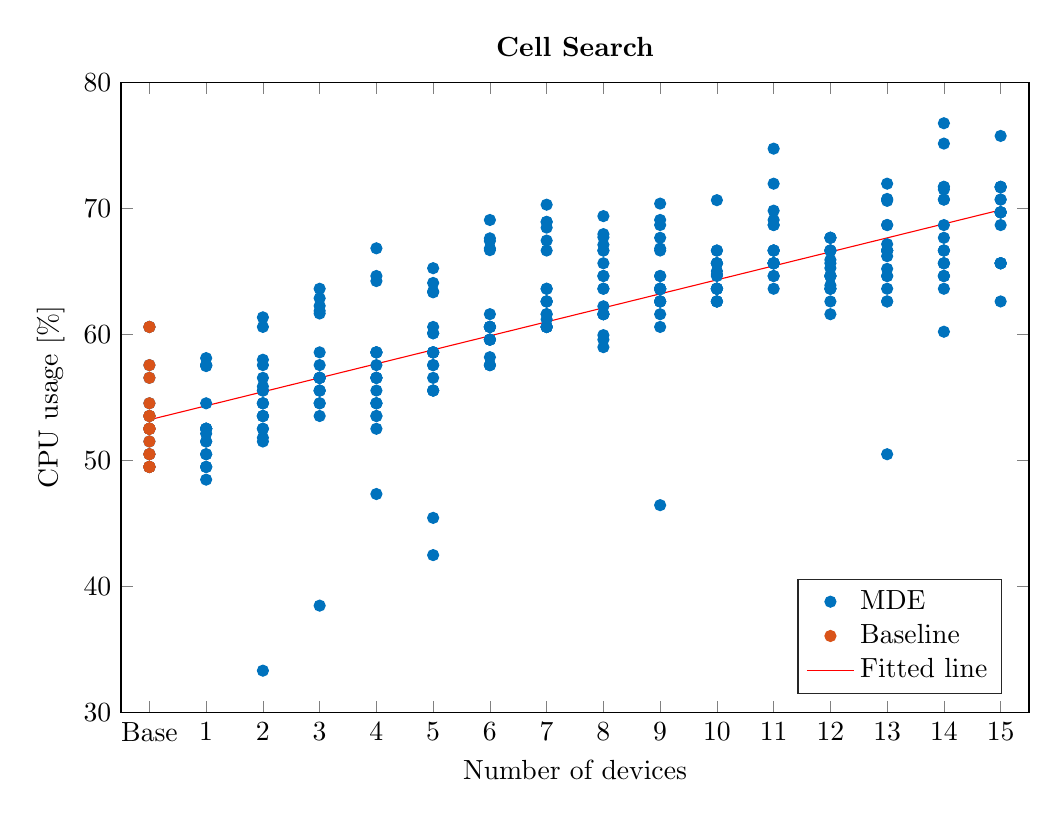
\begin{tikzpicture}

\begin{axis}[%
width=0.951\textwidth,
height=0.66\textwidth,
at={(0\textwidth,0\textwidth)},
scale only axis,
xmin=-0.5,
xmax=15.5,
xtick={0,1,2,3,4,5,6,7,8,9,10,11,12,13,14,15},
xticklabels={{Base},{1},{2},{3},{4},{5},{6},{7},{8},{9},{10},{11},{12},{13},{14},{15}},
xlabel={Number of devices},
ymin=30,
ymax=80,
ylabel={CPU usage [\%]},
axis background/.style={fill=white},
title style={font=\bfseries},
title={Cell Search},
legend style={at={(0.97,0.03)},anchor=south east,legend cell align=left,align=left,draw=white!15!black},
y tick label style={/pgf/number format/fixed}
]
\addplot [color=mycolor1,only marks,mark=*,mark options={solid}]
  table[row sep=crcr]{%
0	49.4966666666667\\
1	48.4866666666667\\
2	51.8133333333333\\
3	53.5366666666667\\
4	58.5833333333333\\
5	63.3504761904762\\
6	58.2033333333333\\
7	68.9375\\
8	61.6166666666667\\
9	62.6266666666667\\
10	63.6333333333333\\
11	65.6566666666667\\
12	64.6466666666667\\
13	71.972\\
14	64.6466666666667\\
15	71.72\\
0	52.5266666666667\\
1	51.5133333333333\\
2	57.5766666666667\\
3	55.5533333333333\\
4	53.5366666666667\\
5	58.5866666666667\\
6	57.5766666666667\\
7	61.2033333333333\\
8	59.5966666666667\\
9	63.6366666666667\\
10	64.7933333333333\\
11	68.69\\
12	64.6466666666667\\
13	66.6666666666667\\
14	66.6666666666667\\
15	69.7\\
0	57.5733333333333\\
1	52.14\\
2	55.5533333333333\\
3	56.5633333333333\\
4	55.5566666666667\\
5	58.5866666666667\\
6	69.09\\
7	68.94\\
8	64.6466666666667\\
9	69.0935\\
10	65.6566666666667\\
11	65.6566666666667\\
12	62.6233333333333\\
14	75.152\\
15	65.6533333333333\\
0	53.5366666666667\\
1	50.5033333333333\\
2	53.5333333333333\\
3	56.5633333333333\\
4	64.6466666666667\\
5	58.5833333333333\\
6	61.6166666666667\\
7	66.6666666666667\\
8	66.6666666666667\\
9	66.828\\
10	62.6233333333333\\
11	66.6666666666667\\
12	65.2733333333333\\
13	70.76\\
14	71.72\\
15	62.6266666666667\\
0	52.5233333333333\\
1	57.4975675675675\\
2	58.0006976744186\\
3	56.5633333333333\\
4	47.34625\\
5	45.4533333333333\\
6	59.5966666666667\\
7	60.6033333333333\\
8	66.6633333333333\\
9	63.6366666666667\\
10	65.6533333333333\\
11	71.97\\
12	66.6666666666667\\
13	66.6666666666667\\
14	70.71\\
15	71.6685\\
0	54.5466666666667\\
1	57.5742857142857\\
2	60.6075\\
3	56.5633333333333\\
4	56.5633333333333\\
5	58.5866666666667\\
6	67.6336363636363\\
7	63.6333333333333\\
8	59.9533333333333\\
9	63.5766666666667\\
10	63.6366666666667\\
11	66.6666666666667\\
12	63.6366666666667\\
13	64.6433333333333\\
14	70.71\\
15	65.6566666666667\\
0	49.4966666666667\\
1	51.5133333333333\\
2	53.5366666666667\\
3	62.275\\
4	56.5666666666667\\
5	55.5566666666667\\
6	59.5933333333333\\
7	62.6233333333333\\
8	65.6566666666667\\
9	64.6466666666667\\
10	66.6633333333333\\
11	68.69\\
12	61.6133333333333\\
13	62.6266666666667\\
14	65.6566666666667\\
15	69.6966666666667\\
0	60.6033333333333\\
1	54.5433333333333\\
2	33.33\\
3	61.879\\
4	56.5633333333333\\
5	58.5833333333333\\
6	59.5966666666667\\
7	70.304\\
9	62.6233333333333\\
10	62.6233333333333\\
11	66.6666666666667\\
12	63.6333333333333\\
13	68.69\\
14	65.6533333333334\\
15	65.6566666666667\\
0	49.4966666666667\\
1	58.13\\
2	55.8804\\
3	58.5866666666667\\
4	57.5733333333333\\
5	60.6033333333333\\
6	57.5733333333333\\
7	62.6266666666667\\
8	61.6133333333333\\
9	67.6766666666667\\
10	63.6366666666667\\
11	63.6333333333333\\
12	65.9233333333333\\
13	68.69\\
14	71.72\\
15	69.7\\
0	51.5166666666667\\
1	52.5233333333333\\
2	54.5433333333333\\
3	61.67\\
4	52.5233333333333\\
5	63.424347826087\\
6	60.6066666666667\\
7	61.6166666666667\\
8	61.6166666666667\\
9	70.3894736842105\\
10	65.6533333333333\\
11	69.83\\
12	64.6433333333333\\
13	67.1733333333333\\
14	68.6866666666667\\
15	71.72\\
0	50.5066666666667\\
1	49.4966666666667\\
2	53.5333333333333\\
3	55.5533333333333\\
4	54.5466666666667\\
5	42.4992857142857\\
6	60.6033333333333\\
7	62.6266666666667\\
8	59\\
9	63.6333333333333\\
10	63.6333333333333\\
11	65.6566666666667\\
12	67.68\\
13	63.6366666666667\\
14	66.6666666666667\\
15	69.6966666666667\\
0	53.5366666666667\\
1	49.4933333333333\\
2	54.5433333333333\\
3	57.5766666666667\\
4	58.5866666666667\\
5	64.094\\
6	60.6066666666667\\
7	68.486\\
8	67.7205\\
9	68.69\\
10	62.6266666666667\\
11	74.75\\
12	66.6666666666667\\
13	62.6266666666667\\
14	76.7666666666667\\
15	75.76\\
0	52.5233333333333\\
1	52.5233333333333\\
2	53.5333333333333\\
3	62.8815\\
4	58.5833333333333\\
5	65.2655\\
6	59.5966666666667\\
7	63.6333333333333\\
8	67.9676190476191\\
9	64.6433333333333\\
10	64.6466666666667\\
11	69.092\\
12	66.668\\
13	66.6666666666667\\
14	64.6433333333333\\
15	65.6566666666667\\
0	56.5666666666667\\
1	52.5233333333333\\
2	61.3655\\
3	54.5433333333333\\
4	58.5866666666667\\
5	57.5766666666667\\
6	60.6066666666667\\
7	60.6033333333333\\
8	69.3965\\
9	60.6033333333333\\
10	63.6366666666667\\
11	64.6466666666667\\
12	66.6666666666667\\
13	70.71\\
14	63.6333333333333\\
15	70.71\\
0	52.5266666666667\\
1	57.5766666666667\\
2	52.5233333333333\\
3	38.49\\
4	66.8433333333333\\
5	60.1\\
6	60.6066666666667\\
7	67.458\\
8	62.24\\
9	46.4633333333333\\
10	62.6233333333333\\
11	65.6533333333333\\
12	67.6766666666667\\
13	66.22\\
14	65.6566666666667\\
15	71.72\\
0	60.6033333333333\\
1	49.4966666666667\\
2	52.5266666666667\\
3	63.6333333333333\\
4	56.5666666666667\\
5	55.5566666666667\\
6	57.5733333333333\\
7	60.6033333333333\\
8	64.6466666666667\\
9	66.6666666666667\\
10	65.03\\
11	65.6566666666667\\
12	67.68\\
13	64.6466666666667\\
14	60.2233333333333\\
15	69.7\\
0	52.5233333333333\\
1	57.5733333333333\\
2	51.5133333333333\\
3	54.5466666666667\\
4	64.244\\
5	56.5633333333333\\
6	67.425\\
7	61.6166666666667\\
8	61.6133333333333\\
9	63.6366666666667\\
10	66.6666666666667\\
11	65.6566666666667\\
12	63.9033333333333\\
13	66.6633333333333\\
14	67.6766666666667\\
15	65.6566666666667\\
0	49.4966666666667\\
1	52.5266666666667\\
2	56.5633333333333\\
3	56.5666666666667\\
4	54.5466666666667\\
5	55.5533333333333\\
6	66.8436363636364\\
7	62.6266666666667\\
8	67.124\\
9	62.6266666666667\\
10	70.662\\
11	65.6533333333334\\
12	64.6433333333333\\
13	65.21\\
14	66.6666666666667\\
15	69.7\\
0	50.5066666666667\\
1	52.5266666666667\\
2	55.5566666666667\\
3	55.5533333333333\\
4	53.5366666666667\\
5	57.5733333333333\\
6	66.6983783783784\\
7	60.6033333333333\\
8	63.6366666666667\\
9	61.6133333333333\\
10	63.6366666666667\\
11	64.6433333333333\\
12	65.6566666666667\\
13	50.5033333333333\\
14	64.6466666666667\\
15	68.6866666666667\\
0	53.5366666666667\\
1	50.5033333333333\\
2	54.5466666666667\\
3	56.5666666666667\\
4	54.5433333333333\\
5	60.1016666666667\\
6	60.6033333333333\\
7	60.6066666666667\\
8	63.6366666666667\\
9	62.6266666666667\\
10	65.6566666666667\\
11	66.67\\
12	63.6366666666667\\
13	70.6085\\
14	71.516\\
15	70.71\\
};
\addlegendentry{MDE};

\addplot [color=mycolor2,only marks,mark=*,mark options={solid}]
  table[row sep=crcr]{%
0	49.4966666666667\\
0	52.5266666666667\\
0	57.5733333333333\\
0	53.5366666666667\\
0	52.5233333333333\\
0	54.5466666666667\\
0	49.4966666666667\\
0	60.6033333333333\\
0	49.4966666666667\\
0	51.5166666666667\\
0	50.5066666666667\\
0	53.5366666666667\\
0	52.5233333333333\\
0	56.5666666666667\\
0	52.5266666666667\\
0	60.6033333333333\\
0	52.5233333333333\\
0	49.4966666666667\\
0	50.5066666666667\\
0	53.5366666666667\\
};
\addlegendentry{Baseline};

\addplot [color=red,solid]
  table[row sep=crcr]{%
0	53.2363131267132\\
0.015	53.2529666207037\\
0.03	53.2696201146943\\
0.045	53.2862736086848\\
0.06	53.3029271026753\\
0.075	53.3195805966658\\
0.09	53.3362340906563\\
0.105	53.3528875846469\\
0.12	53.3695410786374\\
0.135	53.3861945726279\\
0.15	53.4028480666184\\
0.165	53.4195015606089\\
0.18	53.4361550545995\\
0.195	53.45280854859\\
0.21	53.4694620425805\\
0.225	53.486115536571\\
0.24	53.5027690305615\\
0.255	53.5194225245521\\
0.27	53.5360760185426\\
0.285	53.5527295125331\\
0.3	53.5693830065236\\
0.315	53.5860365005141\\
0.33	53.6026899945047\\
0.345	53.6193434884952\\
0.36	53.6359969824857\\
0.375	53.6526504764762\\
0.39	53.6693039704667\\
0.405	53.6859574644573\\
0.42	53.7026109584478\\
0.435	53.7192644524383\\
0.45	53.7359179464288\\
0.465	53.7525714404193\\
0.48	53.7692249344099\\
0.495	53.7858784284004\\
0.51	53.8025319223909\\
0.525	53.8191854163814\\
0.54	53.8358389103719\\
0.555	53.8524924043625\\
0.57	53.869145898353\\
0.585	53.8857993923435\\
0.6	53.902452886334\\
0.615	53.9191063803245\\
0.63	53.9357598743151\\
0.645	53.9524133683056\\
0.66	53.9690668622961\\
0.675	53.9857203562866\\
0.69	54.0023738502771\\
0.705	54.0190273442677\\
0.72	54.0356808382582\\
0.735	54.0523343322487\\
0.75	54.0689878262392\\
0.765	54.0856413202297\\
0.78	54.1022948142203\\
0.795	54.1189483082108\\
0.81	54.1356018022013\\
0.825	54.1522552961918\\
0.84	54.1689087901823\\
0.855	54.1855622841729\\
0.87	54.2022157781634\\
0.885	54.2188692721539\\
0.9	54.2355227661444\\
0.915	54.2521762601349\\
0.93	54.2688297541255\\
0.945	54.285483248116\\
0.96	54.3021367421065\\
0.975	54.318790236097\\
0.99	54.3354437300875\\
1.005	54.3520972240781\\
1.02	54.3687507180686\\
1.035	54.3854042120591\\
1.05	54.4020577060496\\
1.065	54.4187112000401\\
1.08	54.4353646940307\\
1.095	54.4520181880212\\
1.11	54.4686716820117\\
1.125	54.4853251760022\\
1.14	54.5019786699927\\
1.155	54.5186321639833\\
1.17	54.5352856579738\\
1.185	54.5519391519643\\
1.2	54.5685926459548\\
1.215	54.5852461399453\\
1.23	54.6018996339359\\
1.245	54.6185531279264\\
1.26	54.6352066219169\\
1.275	54.6518601159074\\
1.29	54.6685136098979\\
1.305	54.6851671038885\\
1.32	54.701820597879\\
1.335	54.7184740918695\\
1.35	54.73512758586\\
1.365	54.7517810798505\\
1.38	54.7684345738411\\
1.395	54.7850880678316\\
1.41	54.8017415618221\\
1.425	54.8183950558126\\
1.44	54.8350485498031\\
1.455	54.8517020437937\\
1.47	54.8683555377842\\
1.485	54.8850090317747\\
1.5	54.9016625257652\\
1.515	54.9183160197557\\
1.53	54.9349695137463\\
1.545	54.9516230077368\\
1.56	54.9682765017273\\
1.575	54.9849299957178\\
1.59	55.0015834897083\\
1.605	55.0182369836989\\
1.62	55.0348904776894\\
1.635	55.0515439716799\\
1.65	55.0681974656704\\
1.665	55.0848509596609\\
1.68	55.1015044536515\\
1.695	55.118157947642\\
1.71	55.1348114416325\\
1.725	55.151464935623\\
1.74	55.1681184296135\\
1.755	55.1847719236041\\
1.77	55.2014254175946\\
1.785	55.2180789115851\\
1.8	55.2347324055756\\
1.815	55.2513858995661\\
1.83	55.2680393935567\\
1.845	55.2846928875472\\
1.86	55.3013463815377\\
1.875	55.3179998755282\\
1.89	55.3346533695187\\
1.905	55.3513068635093\\
1.92	55.3679603574998\\
1.935	55.3846138514903\\
1.95	55.4012673454808\\
1.965	55.4179208394713\\
1.98	55.4345743334619\\
1.995	55.4512278274524\\
2.01	55.4678813214429\\
2.025	55.4845348154334\\
2.04	55.5011883094239\\
2.055	55.5178418034145\\
2.07	55.534495297405\\
2.085	55.5511487913955\\
2.1	55.567802285386\\
2.115	55.5844557793765\\
2.13	55.6011092733671\\
2.145	55.6177627673576\\
2.16	55.6344162613481\\
2.175	55.6510697553386\\
2.19	55.6677232493291\\
2.205	55.6843767433197\\
2.22	55.7010302373102\\
2.235	55.7176837313007\\
2.25	55.7343372252912\\
2.265	55.7509907192817\\
2.28	55.7676442132723\\
2.295	55.7842977072628\\
2.31	55.8009512012533\\
2.325	55.8176046952438\\
2.34	55.8342581892343\\
2.355	55.8509116832249\\
2.37	55.8675651772154\\
2.385	55.8842186712059\\
2.4	55.9008721651964\\
2.415	55.9175256591869\\
2.43	55.9341791531775\\
2.445	55.950832647168\\
2.46	55.9674861411585\\
2.475	55.984139635149\\
2.49	56.0007931291395\\
2.505	56.0174466231301\\
2.52	56.0341001171206\\
2.535	56.0507536111111\\
2.55	56.0674071051016\\
2.565	56.0840605990921\\
2.58	56.1007140930827\\
2.595	56.1173675870732\\
2.61	56.1340210810637\\
2.625	56.1506745750542\\
2.64	56.1673280690447\\
2.655	56.1839815630353\\
2.67	56.2006350570258\\
2.685	56.2172885510163\\
2.7	56.2339420450068\\
2.715	56.2505955389973\\
2.73	56.2672490329879\\
2.745	56.2839025269784\\
2.76	56.3005560209689\\
2.775	56.3172095149594\\
2.79	56.3338630089499\\
2.805	56.3505165029405\\
2.82	56.367169996931\\
2.835	56.3838234909215\\
2.85	56.400476984912\\
2.865	56.4171304789025\\
2.88	56.4337839728931\\
2.895	56.4504374668836\\
2.91	56.4670909608741\\
2.925	56.4837444548646\\
2.94	56.5003979488551\\
2.955	56.5170514428457\\
2.97	56.5337049368362\\
2.985	56.5503584308267\\
3	56.5670119248172\\
3.015	56.5836654188077\\
3.03	56.6003189127983\\
3.045	56.6169724067888\\
3.06	56.6336259007793\\
3.075	56.6502793947698\\
3.09	56.6669328887603\\
3.105	56.6835863827509\\
3.12	56.7002398767414\\
3.135	56.7168933707319\\
3.15	56.7335468647224\\
3.165	56.7502003587129\\
3.18	56.7668538527034\\
3.195	56.783507346694\\
3.21	56.8001608406845\\
3.225	56.816814334675\\
3.24	56.8334678286655\\
3.255	56.8501213226561\\
3.27	56.8667748166466\\
3.285	56.8834283106371\\
3.3	56.9000818046276\\
3.315	56.9167352986181\\
3.33	56.9333887926087\\
3.345	56.9500422865992\\
3.36	56.9666957805897\\
3.375	56.9833492745802\\
3.39	57.0000027685707\\
3.405	57.0166562625612\\
3.42	57.0333097565518\\
3.435	57.0499632505423\\
3.45	57.0666167445328\\
3.465	57.0832702385233\\
3.48	57.0999237325139\\
3.495	57.1165772265044\\
3.51	57.1332307204949\\
3.525	57.1498842144854\\
3.54	57.1665377084759\\
3.555	57.1831912024665\\
3.57	57.199844696457\\
3.585	57.2164981904475\\
3.6	57.233151684438\\
3.615	57.2498051784285\\
3.63	57.266458672419\\
3.645	57.2831121664096\\
3.66	57.2997656604001\\
3.675	57.3164191543906\\
3.69	57.3330726483811\\
3.705	57.3497261423717\\
3.72	57.3663796363622\\
3.735	57.3830331303527\\
3.75	57.3996866243432\\
3.765	57.4163401183337\\
3.78	57.4329936123243\\
3.795	57.4496471063148\\
3.81	57.4663006003053\\
3.825	57.4829540942958\\
3.84	57.4996075882863\\
3.855	57.5162610822768\\
3.87	57.5329145762674\\
3.885	57.5495680702579\\
3.9	57.5662215642484\\
3.915	57.5828750582389\\
3.93	57.5995285522295\\
3.945	57.61618204622\\
3.96	57.6328355402105\\
3.975	57.649489034201\\
3.99	57.6661425281915\\
4.005	57.682796022182\\
4.02	57.6994495161726\\
4.035	57.7161030101631\\
4.05	57.7327565041536\\
4.065	57.7494099981441\\
4.08	57.7660634921346\\
4.095	57.7827169861252\\
4.11	57.7993704801157\\
4.125	57.8160239741062\\
4.14	57.8326774680967\\
4.155	57.8493309620873\\
4.17	57.8659844560778\\
4.185	57.8826379500683\\
4.2	57.8992914440588\\
4.215	57.9159449380493\\
4.23	57.9325984320398\\
4.245	57.9492519260304\\
4.26	57.9659054200209\\
4.275	57.9825589140114\\
4.29	57.9992124080019\\
4.305	58.0158659019924\\
4.32	58.032519395983\\
4.335	58.0491728899735\\
4.35	58.065826383964\\
4.365	58.0824798779545\\
4.38	58.0991333719451\\
4.395	58.1157868659356\\
4.41	58.1324403599261\\
4.425	58.1490938539166\\
4.44	58.1657473479071\\
4.455	58.1824008418976\\
4.47	58.1990543358882\\
4.485	58.2157078298787\\
4.5	58.2323613238692\\
4.515	58.2490148178597\\
4.53	58.2656683118502\\
4.545	58.2823218058408\\
4.56	58.2989752998313\\
4.575	58.3156287938218\\
4.59	58.3322822878123\\
4.605	58.3489357818029\\
4.62	58.3655892757934\\
4.635	58.3822427697839\\
4.65	58.3988962637744\\
4.665	58.4155497577649\\
4.68	58.4322032517554\\
4.695	58.448856745746\\
4.71	58.4655102397365\\
4.725	58.482163733727\\
4.74	58.4988172277175\\
4.755	58.515470721708\\
4.77	58.5321242156986\\
4.785	58.5487777096891\\
4.8	58.5654312036796\\
4.815	58.5820846976701\\
4.83	58.5987381916607\\
4.845	58.6153916856512\\
4.86	58.6320451796417\\
4.875	58.6486986736322\\
4.89	58.6653521676227\\
4.905	58.6820056616132\\
4.92	58.6986591556038\\
4.935	58.7153126495943\\
4.95	58.7319661435848\\
4.965	58.7486196375753\\
4.98	58.7652731315658\\
4.995	58.7819266255564\\
5.01	58.7985801195469\\
5.025	58.8152336135374\\
5.04	58.8318871075279\\
5.055	58.8485406015184\\
5.07	58.865194095509\\
5.085	58.8818475894995\\
5.1	58.89850108349\\
5.115	58.9151545774805\\
5.13	58.931808071471\\
5.145	58.9484615654616\\
5.16	58.9651150594521\\
5.175	58.9817685534426\\
5.19	58.9984220474331\\
5.205	59.0150755414236\\
5.22	59.0317290354142\\
5.235	59.0483825294047\\
5.25	59.0650360233952\\
5.265	59.0816895173857\\
5.28	59.0983430113762\\
5.295	59.1149965053668\\
5.31	59.1316499993573\\
5.325	59.1483034933478\\
5.34	59.1649569873383\\
5.355	59.1816104813288\\
5.37	59.1982639753194\\
5.385	59.2149174693099\\
5.4	59.2315709633004\\
5.415	59.2482244572909\\
5.43	59.2648779512814\\
5.445	59.281531445272\\
5.46	59.2981849392625\\
5.475	59.314838433253\\
5.49	59.3314919272435\\
5.505	59.348145421234\\
5.52	59.3647989152246\\
5.535	59.3814524092151\\
5.55	59.3981059032056\\
5.565	59.4147593971961\\
5.58	59.4314128911866\\
5.595	59.4480663851772\\
5.61	59.4647198791677\\
5.625	59.4813733731582\\
5.64	59.4980268671487\\
5.655	59.5146803611392\\
5.67	59.5313338551298\\
5.685	59.5479873491203\\
5.7	59.5646408431108\\
5.715	59.5812943371013\\
5.73	59.5979478310918\\
5.745	59.6146013250824\\
5.76	59.6312548190729\\
5.775	59.6479083130634\\
5.79	59.6645618070539\\
5.805	59.6812153010444\\
5.82	59.697868795035\\
5.835	59.7145222890255\\
5.85	59.731175783016\\
5.865	59.7478292770065\\
5.88	59.764482770997\\
5.895	59.7811362649876\\
5.91	59.7977897589781\\
5.925	59.8144432529686\\
5.94	59.8310967469591\\
5.955	59.8477502409496\\
5.97	59.8644037349402\\
5.985	59.8810572289307\\
6	59.8977107229212\\
6.015	59.9143642169117\\
6.03	59.9310177109022\\
6.045	59.9476712048928\\
6.06	59.9643246988833\\
6.075	59.9809781928738\\
6.09	59.9976316868643\\
6.105	60.0142851808548\\
6.12	60.0309386748454\\
6.135	60.0475921688359\\
6.15	60.0642456628264\\
6.165	60.0808991568169\\
6.18	60.0975526508074\\
6.195	60.114206144798\\
6.21	60.1308596387885\\
6.225	60.147513132779\\
6.24	60.1641666267695\\
6.255	60.18082012076\\
6.27	60.1974736147506\\
6.285	60.2141271087411\\
6.3	60.2307806027316\\
6.315	60.2474340967221\\
6.33	60.2640875907126\\
6.345	60.2807410847032\\
6.36	60.2973945786937\\
6.375	60.3140480726842\\
6.39	60.3307015666747\\
6.405	60.3473550606652\\
6.42	60.3640085546558\\
6.435	60.3806620486463\\
6.45	60.3973155426368\\
6.465	60.4139690366273\\
6.48	60.4306225306178\\
6.495	60.4472760246084\\
6.51	60.4639295185989\\
6.525	60.4805830125894\\
6.54	60.4972365065799\\
6.555	60.5138900005704\\
6.57	60.530543494561\\
6.585	60.5471969885515\\
6.6	60.563850482542\\
6.615	60.5805039765325\\
6.63	60.597157470523\\
6.645	60.6138109645136\\
6.66	60.6304644585041\\
6.675	60.6471179524946\\
6.69	60.6637714464851\\
6.705	60.6804249404756\\
6.72	60.6970784344662\\
6.735	60.7137319284567\\
6.75	60.7303854224472\\
6.765	60.7470389164377\\
6.78	60.7636924104282\\
6.795	60.7803459044188\\
6.81	60.7969993984093\\
6.825	60.8136528923998\\
6.84	60.8303063863903\\
6.855	60.8469598803808\\
6.87	60.8636133743714\\
6.885	60.8802668683619\\
6.9	60.8969203623524\\
6.915	60.9135738563429\\
6.93	60.9302273503334\\
6.945	60.946880844324\\
6.96	60.9635343383145\\
6.975	60.980187832305\\
6.99	60.9968413262955\\
7.005	61.013494820286\\
7.02	61.0301483142766\\
7.035	61.0468018082671\\
7.05	61.0634553022576\\
7.065	61.0801087962481\\
7.08	61.0967622902386\\
7.095	61.1134157842292\\
7.11	61.1300692782197\\
7.125	61.1467227722102\\
7.14	61.1633762662007\\
7.155	61.1800297601912\\
7.17	61.1966832541818\\
7.185	61.2133367481723\\
7.2	61.2299902421628\\
7.215	61.2466437361533\\
7.23	61.2632972301438\\
7.245	61.2799507241344\\
7.26	61.2966042181249\\
7.275	61.3132577121154\\
7.29	61.3299112061059\\
7.305	61.3465647000964\\
7.32	61.363218194087\\
7.335	61.3798716880775\\
7.35	61.396525182068\\
7.365	61.4131786760585\\
7.38	61.429832170049\\
7.395	61.4464856640396\\
7.41	61.4631391580301\\
7.425	61.4797926520206\\
7.44	61.4964461460111\\
7.455	61.5130996400016\\
7.47	61.5297531339922\\
7.485	61.5464066279827\\
7.5	61.5630601219732\\
7.515	61.5797136159637\\
7.53	61.5963671099542\\
7.545	61.6130206039448\\
7.56	61.6296740979353\\
7.575	61.6463275919258\\
7.59	61.6629810859163\\
7.605	61.6796345799068\\
7.62	61.6962880738974\\
7.635	61.7129415678879\\
7.65	61.7295950618784\\
7.665	61.7462485558689\\
7.68	61.7629020498594\\
7.695	61.77955554385\\
7.71	61.7962090378405\\
7.725	61.812862531831\\
7.74	61.8295160258215\\
7.755	61.846169519812\\
7.77	61.8628230138026\\
7.785	61.8794765077931\\
7.8	61.8961300017836\\
7.815	61.9127834957741\\
7.83	61.9294369897646\\
7.845	61.9460904837552\\
7.86	61.9627439777457\\
7.875	61.9793974717362\\
7.89	61.9960509657267\\
7.905	62.0127044597172\\
7.92	62.0293579537078\\
7.935	62.0460114476983\\
7.95	62.0626649416888\\
7.965	62.0793184356793\\
7.98	62.0959719296698\\
7.995	62.1126254236604\\
8.01	62.1292789176509\\
8.025	62.1459324116414\\
8.04	62.1625859056319\\
8.055	62.1792393996224\\
8.07	62.195892893613\\
8.085	62.2125463876035\\
8.1	62.229199881594\\
8.115	62.2458533755845\\
8.13	62.262506869575\\
8.145	62.2791603635656\\
8.16	62.2958138575561\\
8.175	62.3124673515466\\
8.19	62.3291208455371\\
8.205	62.3457743395276\\
8.22	62.3624278335182\\
8.235	62.3790813275087\\
8.25	62.3957348214992\\
8.265	62.4123883154897\\
8.28	62.4290418094802\\
8.295	62.4456953034708\\
8.31	62.4623487974613\\
8.325	62.4790022914518\\
8.34	62.4956557854423\\
8.355	62.5123092794328\\
8.37	62.5289627734234\\
8.385	62.5456162674139\\
8.4	62.5622697614044\\
8.415	62.5789232553949\\
8.43	62.5955767493854\\
8.445	62.612230243376\\
8.46	62.6288837373665\\
8.475	62.645537231357\\
8.49	62.6621907253475\\
8.505	62.678844219338\\
8.52	62.6954977133286\\
8.535	62.7121512073191\\
8.55	62.7288047013096\\
8.565	62.7454581953001\\
8.58	62.7621116892906\\
8.595	62.7787651832812\\
8.61	62.7954186772717\\
8.625	62.8120721712622\\
8.64	62.8287256652527\\
8.655	62.8453791592432\\
8.67	62.8620326532338\\
8.685	62.8786861472243\\
8.7	62.8953396412148\\
8.715	62.9119931352053\\
8.73	62.9286466291958\\
8.745	62.9453001231864\\
8.76	62.9619536171769\\
8.775	62.9786071111674\\
8.79	62.9952606051579\\
8.805	63.0119140991484\\
8.82	63.028567593139\\
8.835	63.0452210871295\\
8.85	63.06187458112\\
8.865	63.0785280751105\\
8.88	63.095181569101\\
8.895	63.1118350630916\\
8.91	63.1284885570821\\
8.925	63.1451420510726\\
8.94	63.1617955450631\\
8.955	63.1784490390536\\
8.97	63.1951025330442\\
8.985	63.2117560270347\\
9	63.2284095210252\\
9.015	63.2450630150157\\
9.03	63.2617165090062\\
9.045	63.2783700029968\\
9.06	63.2950234969873\\
9.075	63.3116769909778\\
9.09	63.3283304849683\\
9.105	63.3449839789588\\
9.12	63.3616374729494\\
9.135	63.3782909669399\\
9.15	63.3949444609304\\
9.165	63.4115979549209\\
9.18	63.4282514489114\\
9.195	63.444904942902\\
9.21	63.4615584368925\\
9.225	63.478211930883\\
9.24	63.4948654248735\\
9.255	63.511518918864\\
9.27	63.5281724128546\\
9.285	63.5448259068451\\
9.3	63.5614794008356\\
9.315	63.5781328948261\\
9.33	63.5947863888166\\
9.345	63.6114398828072\\
9.36	63.6280933767977\\
9.375	63.6447468707882\\
9.39	63.6614003647787\\
9.405	63.6780538587692\\
9.42	63.6947073527598\\
9.435	63.7113608467503\\
9.45	63.7280143407408\\
9.465	63.7446678347313\\
9.48	63.7613213287218\\
9.495	63.7779748227124\\
9.51	63.7946283167029\\
9.525	63.8112818106934\\
9.54	63.8279353046839\\
9.555	63.8445887986744\\
9.57	63.861242292665\\
9.585	63.8778957866555\\
9.6	63.894549280646\\
9.615	63.9112027746365\\
9.63	63.927856268627\\
9.645	63.9445097626176\\
9.66	63.9611632566081\\
9.675	63.9778167505986\\
9.69	63.9944702445891\\
9.705	64.0111237385796\\
9.72	64.0277772325702\\
9.735	64.0444307265607\\
9.75	64.0610842205512\\
9.765	64.0777377145417\\
9.78	64.0943912085322\\
9.795	64.1110447025227\\
9.81	64.1276981965133\\
9.825	64.1443516905038\\
9.84	64.1610051844943\\
9.855	64.1776586784848\\
9.87	64.1943121724754\\
9.885	64.2109656664659\\
9.9	64.2276191604564\\
9.915	64.2442726544469\\
9.93	64.2609261484374\\
9.945	64.277579642428\\
9.96	64.2942331364185\\
9.975	64.310886630409\\
9.99	64.3275401243995\\
10.005	64.34419361839\\
10.02	64.3608471123806\\
10.035	64.3775006063711\\
10.05	64.3941541003616\\
10.065	64.4108075943521\\
10.08	64.4274610883426\\
10.095	64.4441145823332\\
10.11	64.4607680763237\\
10.125	64.4774215703142\\
10.14	64.4940750643047\\
10.155	64.5107285582952\\
10.17	64.5273820522858\\
10.185	64.5440355462763\\
10.2	64.5606890402668\\
10.215	64.5773425342573\\
10.23	64.5939960282478\\
10.245	64.6106495222383\\
10.26	64.6273030162289\\
10.275	64.6439565102194\\
10.29	64.6606100042099\\
10.305	64.6772634982004\\
10.32	64.693916992191\\
10.335	64.7105704861815\\
10.35	64.727223980172\\
10.365	64.7438774741625\\
10.38	64.760530968153\\
10.395	64.7771844621436\\
10.41	64.7938379561341\\
10.425	64.8104914501246\\
10.44	64.8271449441151\\
10.455	64.8437984381056\\
10.47	64.8604519320962\\
10.485	64.8771054260867\\
10.5	64.8937589200772\\
10.515	64.9104124140677\\
10.53	64.9270659080582\\
10.545	64.9437194020488\\
10.56	64.9603728960393\\
10.575	64.9770263900298\\
10.59	64.9936798840203\\
10.605	65.0103333780108\\
10.62	65.0269868720013\\
10.635	65.0436403659919\\
10.65	65.0602938599824\\
10.665	65.0769473539729\\
10.68	65.0936008479634\\
10.695	65.1102543419539\\
10.71	65.1269078359445\\
10.725	65.143561329935\\
10.74	65.1602148239255\\
10.755	65.176868317916\\
10.77	65.1935218119066\\
10.785	65.2101753058971\\
10.8	65.2268287998876\\
10.815	65.2434822938781\\
10.83	65.2601357878686\\
10.845	65.2767892818592\\
10.86	65.2934427758497\\
10.875	65.3100962698402\\
10.89	65.3267497638307\\
10.905	65.3434032578212\\
10.92	65.3600567518118\\
10.935	65.3767102458023\\
10.95	65.3933637397928\\
10.965	65.4100172337833\\
10.98	65.4266707277738\\
10.995	65.4433242217644\\
11.01	65.4599777157549\\
11.025	65.4766312097454\\
11.04	65.4932847037359\\
11.055	65.5099381977264\\
11.07	65.526591691717\\
11.085	65.5432451857075\\
11.1	65.559898679698\\
11.115	65.5765521736885\\
11.13	65.593205667679\\
11.145	65.6098591616695\\
11.16	65.6265126556601\\
11.175	65.6431661496506\\
11.19	65.6598196436411\\
11.205	65.6764731376316\\
11.22	65.6931266316222\\
11.235	65.7097801256127\\
11.25	65.7264336196032\\
11.265	65.7430871135937\\
11.28	65.7597406075842\\
11.295	65.7763941015748\\
11.31	65.7930475955653\\
11.325	65.8097010895558\\
11.34	65.8263545835463\\
11.355	65.8430080775368\\
11.37	65.8596615715274\\
11.385	65.8763150655179\\
11.4	65.8929685595084\\
11.415	65.9096220534989\\
11.43	65.9262755474894\\
11.445	65.94292904148\\
11.46	65.9595825354705\\
11.475	65.976236029461\\
11.49	65.9928895234515\\
11.505	66.009543017442\\
11.52	66.0261965114325\\
11.535	66.0428500054231\\
11.55	66.0595034994136\\
11.565	66.0761569934041\\
11.58	66.0928104873946\\
11.595	66.1094639813851\\
11.61	66.1261174753757\\
11.625	66.1427709693662\\
11.64	66.1594244633567\\
11.655	66.1760779573472\\
11.67	66.1927314513378\\
11.685	66.2093849453283\\
11.7	66.2260384393188\\
11.715	66.2426919333093\\
11.73	66.2593454272998\\
11.745	66.2759989212904\\
11.76	66.2926524152809\\
11.775	66.3093059092714\\
11.79	66.3259594032619\\
11.805	66.3426128972524\\
11.82	66.359266391243\\
11.835	66.3759198852335\\
11.85	66.392573379224\\
11.865	66.4092268732145\\
11.88	66.425880367205\\
11.895	66.4425338611956\\
11.91	66.4591873551861\\
11.925	66.4758408491766\\
11.94	66.4924943431671\\
11.955	66.5091478371576\\
11.97	66.5258013311481\\
11.985	66.5424548251387\\
12	66.5591083191292\\
12.015	66.5757618131197\\
12.03	66.5924153071102\\
12.045	66.6090688011007\\
12.06	66.6257222950913\\
12.075	66.6423757890818\\
12.09	66.6590292830723\\
12.105	66.6756827770628\\
12.12	66.6923362710534\\
12.135	66.7089897650439\\
12.15	66.7256432590344\\
12.165	66.7422967530249\\
12.18	66.7589502470154\\
12.195	66.775603741006\\
12.21	66.7922572349965\\
12.225	66.808910728987\\
12.24	66.8255642229775\\
12.255	66.842217716968\\
12.27	66.8588712109585\\
12.285	66.8755247049491\\
12.3	66.8921781989396\\
12.315	66.9088316929301\\
12.33	66.9254851869206\\
12.345	66.9421386809111\\
12.36	66.9587921749017\\
12.375	66.9754456688922\\
12.39	66.9920991628827\\
12.405	67.0087526568732\\
12.42	67.0254061508637\\
12.435	67.0420596448543\\
12.45	67.0587131388448\\
12.465	67.0753666328353\\
12.48	67.0920201268258\\
12.495	67.1086736208163\\
12.51	67.1253271148069\\
12.525	67.1419806087974\\
12.54	67.1586341027879\\
12.555	67.1752875967784\\
12.57	67.191941090769\\
12.585	67.2085945847595\\
12.6	67.22524807875\\
12.615	67.2419015727405\\
12.63	67.258555066731\\
12.645	67.2752085607216\\
12.66	67.2918620547121\\
12.675	67.3085155487026\\
12.69	67.3251690426931\\
12.705	67.3418225366836\\
12.72	67.3584760306741\\
12.735	67.3751295246647\\
12.75	67.3917830186552\\
12.765	67.4084365126457\\
12.78	67.4250900066362\\
12.795	67.4417435006267\\
12.81	67.4583969946173\\
12.825	67.4750504886078\\
12.84	67.4917039825983\\
12.855	67.5083574765888\\
12.87	67.5250109705793\\
12.885	67.5416644645699\\
12.9	67.5583179585604\\
12.915	67.5749714525509\\
12.93	67.5916249465414\\
12.945	67.6082784405319\\
12.96	67.6249319345225\\
12.975	67.641585428513\\
12.99	67.6582389225035\\
13.005	67.674892416494\\
13.02	67.6915459104846\\
13.035	67.7081994044751\\
13.05	67.7248528984656\\
13.065	67.7415063924561\\
13.08	67.7581598864466\\
13.095	67.7748133804371\\
13.11	67.7914668744277\\
13.125	67.8081203684182\\
13.14	67.8247738624087\\
13.155	67.8414273563992\\
13.17	67.8580808503897\\
13.185	67.8747343443803\\
13.2	67.8913878383708\\
13.215	67.9080413323613\\
13.23	67.9246948263518\\
13.245	67.9413483203423\\
13.26	67.9580018143329\\
13.275	67.9746553083234\\
13.29	67.9913088023139\\
13.305	68.0079622963044\\
13.32	68.0246157902949\\
13.335	68.0412692842855\\
13.35	68.057922778276\\
13.365	68.0745762722665\\
13.38	68.091229766257\\
13.395	68.1078832602475\\
13.41	68.1245367542381\\
13.425	68.1411902482286\\
13.44	68.1578437422191\\
13.455	68.1744972362096\\
13.47	68.1911507302002\\
13.485	68.2078042241907\\
13.5	68.2244577181812\\
13.515	68.2411112121717\\
13.53	68.2577647061622\\
13.545	68.2744182001528\\
13.56	68.2910716941433\\
13.575	68.3077251881338\\
13.59	68.3243786821243\\
13.605	68.3410321761148\\
13.62	68.3576856701053\\
13.635	68.3743391640959\\
13.65	68.3909926580864\\
13.665	68.4076461520769\\
13.68	68.4242996460674\\
13.695	68.4409531400579\\
13.71	68.4576066340485\\
13.725	68.474260128039\\
13.74	68.4909136220295\\
13.755	68.50756711602\\
13.77	68.5242206100105\\
13.785	68.5408741040011\\
13.8	68.5575275979916\\
13.815	68.5741810919821\\
13.83	68.5908345859726\\
13.845	68.6074880799631\\
13.86	68.6241415739537\\
13.875	68.6407950679442\\
13.89	68.6574485619347\\
13.905	68.6741020559252\\
13.92	68.6907555499158\\
13.935	68.7074090439063\\
13.95	68.7240625378968\\
13.965	68.7407160318873\\
13.98	68.7573695258778\\
13.995	68.7740230198683\\
14.01	68.7906765138589\\
14.025	68.8073300078494\\
14.04	68.8239835018399\\
14.055	68.8406369958304\\
14.07	68.8572904898209\\
14.085	68.8739439838115\\
14.1	68.890597477802\\
14.115	68.9072509717925\\
14.13	68.923904465783\\
14.145	68.9405579597735\\
14.16	68.9572114537641\\
14.175	68.9738649477546\\
14.19	68.9905184417451\\
14.205	69.0071719357356\\
14.22	69.0238254297261\\
14.235	69.0404789237167\\
14.25	69.0571324177072\\
14.265	69.0737859116977\\
14.28	69.0904394056882\\
14.295	69.1070928996787\\
14.31	69.1237463936693\\
14.325	69.1403998876598\\
14.34	69.1570533816503\\
14.355	69.1737068756408\\
14.37	69.1903603696314\\
14.385	69.2070138636219\\
14.4	69.2236673576124\\
14.415	69.2403208516029\\
14.43	69.2569743455934\\
14.445	69.2736278395839\\
14.46	69.2902813335745\\
14.475	69.306934827565\\
14.49	69.3235883215555\\
14.505	69.340241815546\\
14.52	69.3568953095365\\
14.535	69.3735488035271\\
14.55	69.3902022975176\\
14.565	69.4068557915081\\
14.58	69.4235092854986\\
14.595	69.4401627794891\\
14.61	69.4568162734797\\
14.625	69.4734697674702\\
14.64	69.4901232614607\\
14.655	69.5067767554512\\
14.67	69.5234302494417\\
14.685	69.5400837434323\\
14.7	69.5567372374228\\
14.715	69.5733907314133\\
14.73	69.5900442254038\\
14.745	69.6066977193943\\
14.76	69.6233512133849\\
14.775	69.6400047073754\\
14.79	69.6566582013659\\
14.805	69.6733116953564\\
14.82	69.6899651893469\\
14.835	69.7066186833375\\
14.85	69.723272177328\\
14.865	69.7399256713185\\
14.88	69.756579165309\\
14.895	69.7732326592995\\
14.91	69.7898861532901\\
14.925	69.8065396472806\\
14.94	69.8231931412711\\
14.955	69.8398466352616\\
14.97	69.8565001292521\\
14.985	69.8731536232427\\
15	69.8898071172332\\
};
\addlegendentry{Fitted line};

\end{axis}
\end{tikzpicture}%}
\caption{CPU usage for the synchronization step of the MDE for different number of devices and the baseline emulator. The fitted line is a linear approximation}
\label{fig:CPU_sync}
\end{figure}

The fitted line for the CPU usage is estimated to be:
\begin{equation}
CPU_{sync} = 1.11 \cdot NoD + 53.24
\end{equation}

As seen on \autoref{fig:CPU_sync}, the average CPU usage is rising with the number of devices. This is a problem, as it will hit full usage at some point, which can effect the ability to synchronize with the cell. The synchronization is performed in a single thread, which sets the limit at 100\%, but the increase in CPU usage could be explained by the higher number of threads that is running in all the higher layer classes of each device, which means the limit could be as high as 700\%. 

\subsection{Decoding of MIB-NB}
The decoding of MIB-NB is measured from just after a cell is found until the MIB-NB has been fully decoded, the average CPU usage of this step is seen on \autoref{fig:CPU_init}. The measurements are showing only the CPU usage of the last attempt at decoding the MIB-NB if multiple attempts was made.

\begin{figure}[H]
\tikzsetnextfilename{CPU_MIB}
\centering
\resizebox{0.5\textwidth}{!}{
% This file was created by matlab2tikz.
%
%The latest updates can be retrieved from
%  http://www.mathworks.com/matlabcentral/fileexchange/22022-matlab2tikz-matlab2tikz
%where you can also make suggestions and rate matlab2tikz.
%
\definecolor{mycolor1}{rgb}{0.00000,0.44700,0.74100}%
\definecolor{mycolor2}{rgb}{0.85000,0.32500,0.09800}%
%
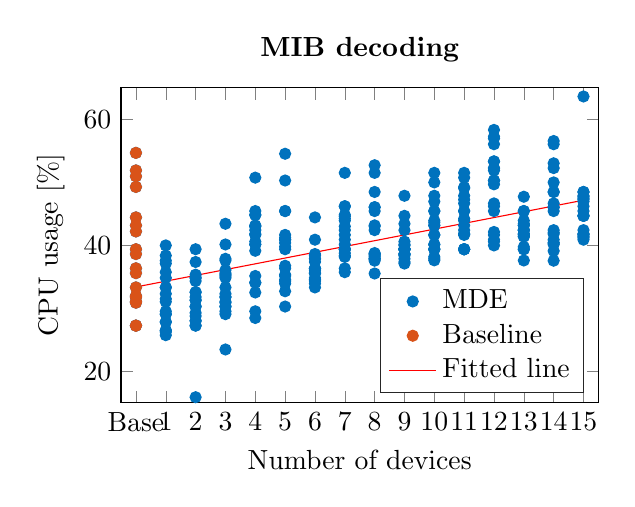
\begin{tikzpicture}

\begin{axis}[%
width=0.5\textwidth,
height=0.33\textwidth,
at={(0\textwidth,0\textwidth)},
scale only axis,
xmin=-0.5,
xmax=15.5,
xtick={0,1,2,3,4,5,6,7,8,9,10,11,12,13,14,15},
xticklabels={{Base},{1},{2},{3},{4},{5},{6},{7},{8},{9},{10},{11},{12},{13},{14},{15}},
xlabel={Number of devices},
ymin=15,
ymax=65,
ylabel={CPU usage [\%]},
axis background/.style={fill=white},
title style={font=\bfseries},
title={MIB decoding},
legend style={at={(0.97,0.03)},anchor=south east,legend cell align=left,align=left,draw=white!15!black},
y tick label style={/pgf/number format/fixed}
]
\addplot [color=mycolor1,only marks,mark=*,mark options={solid}]
  table[row sep=crcr]{%
0	31.9855555555556\\
1	37.574\\
2	39.3933333333333\\
3	29.088\\
4	35.148\\
5	35.148\\
6	36.0725\\
7	39.39\\
8	46.058\\
9	37.875\\
10	43.634\\
11	41.6625\\
12	56.0575\\
13	42.42\\
14	52.27\\
15	48.4825\\
0	31.8175\\
1	26.5125\\
2	31.815\\
3	31.0575\\
4	45.4525\\
5	41.665\\
6	36.36\\
7	46.21\\
8	37.875\\
9	38.6325\\
10	40.1475\\
11	44.24\\
12	51.888\\
13	39.39\\
14	41.814\\
15	44.695\\
0	50.9730769230769\\
1	27.876\\
2	29.29\\
3	35.6025\\
4	40.15\\
5	40.9075\\
6	37.875\\
7	43.028\\
8	46.058\\
9	39.996\\
10	39.39\\
11	49.24\\
12	57.2625\\
14	46.06\\
15	41.208\\
0	27.27\\
1	25.755\\
2	32.5725\\
3	36.0933333333333\\
4	43.028\\
5	33.936\\
6	34.542\\
7	38.784\\
8	43.028\\
9	42.42\\
10	39.39\\
11	39.39\\
12	42.1325\\
13	41.816\\
14	48.4833333333333\\
15	41.41\\
0	31.815\\
1	33.33\\
2	32.5725\\
3	30.3\\
4	41.665\\
5	34.34\\
6	36.36\\
7	43.9375\\
8	45.452\\
9	39.39\\
10	43.1775\\
11	47.27\\
12	53.33\\
13	43.43\\
14	46.058\\
15	44.6925\\
0	43.168947368421\\
1	27.8275\\
2	34.34\\
3	34.845\\
4	29.5425\\
5	39.802\\
6	35.6025\\
7	40.1475\\
8	37.875\\
9	38.6325\\
10	45.4525\\
11	43.1775\\
12	39.996\\
13	43.1775\\
14	46.664\\
15	42.4225\\
0	39.3925\\
1	29.5425\\
2	35.35\\
3	30.906\\
4	39.1475\\
5	45.4525\\
6	34.845\\
7	39.39\\
8	38.784\\
9	37.37\\
10	46.9675\\
11	45.4525\\
12	58.33\\
13	41.41\\
14	56.0575\\
15	44.695\\
0	51.89625\\
1	32.32\\
2	15.9075\\
3	31.815\\
4	32.528\\
5	36.36\\
6	35.6025\\
7	44.24\\
9	39.39\\
10	41.6625\\
11	39.39\\
12	53.33\\
13	45.4533333333333\\
14	42.42\\
15	41.814\\
0	38.635\\
1	26.26\\
2	28.0275\\
3	40.15\\
4	34.0875\\
5	36.77\\
6	34.34\\
7	41.665\\
8	37.572\\
9	40.602\\
10	43.18\\
11	39.39\\
12	50.3\\
13	45.4525\\
14	53.03\\
15	45.452\\
0	33.332\\
1	29.088\\
2	30.3\\
3	43.4333333333333\\
4	50.755\\
5	40.4\\
6	34.542\\
7	42.422\\
8	38.38\\
9	47.876\\
10	43.9375\\
11	45.452\\
12	45.4525\\
13	37.6075\\
14	48.482\\
15	47.725\\
0	54.6859090909091\\
1	38.3833333333333\\
2	28.0275\\
3	35.35\\
4	43.028\\
5	39.3925\\
6	33.936\\
7	38.38\\
8	52.724\\
9	39.39\\
10	40.1475\\
11	42.422\\
12	46.21\\
13	41.41\\
14	56.5666666666667\\
15	63.635\\
0	27.27\\
1	39.998\\
2	27.27\\
3	30.3\\
4	42.4225\\
5	40.9075\\
6	44.4433333333333\\
7	51.5125\\
8	38.6325\\
9	43.4333333333333\\
10	49.9975\\
11	46.666\\
12	52.27\\
13	42.42\\
14	49.9975\\
15	46.9675\\
0	31.0575\\
1	29.088\\
2	37.37\\
3	37.875\\
4	34.0875\\
5	34.542\\
6	36.36\\
7	39.39\\
8	37.875\\
9	44.695\\
10	39.39\\
11	39.39\\
12	40.905\\
13	42.4225\\
14	40.4\\
15	41.814\\
0	44.445\\
1	31.512\\
2	34.845\\
3	32.32\\
4	40.15\\
5	41.21\\
6	37.875\\
7	35.754\\
8	48.4825\\
9	37.1175\\
10	37.875\\
11	51.5125\\
12	49.694\\
13	47.725\\
14	37.572\\
15	48.4825\\
0	36.3625\\
1	37.12\\
2	27.27\\
3	35.15\\
4	44.8275\\
5	30.3\\
6	38.3833333333333\\
7	44.616\\
8	38.178\\
9	38.38\\
10	38.178\\
11	41.814\\
12	56.966\\
13	43.1775\\
14	40.4\\
15	47.272\\
0	42.2178947368421\\
1	35.756\\
2	34.845\\
3	33.33\\
4	43.18\\
5	45.4525\\
6	33.33\\
7	36.36\\
8	42.4225\\
9	40.1475\\
10	37.63\\
11	50.755\\
12	46.664\\
13	41.665\\
14	42.0366666666667\\
15	47.878\\
0	31.0575\\
1	31.0575\\
2	28.785\\
3	29.5425\\
4	41.816\\
5	50.3\\
6	37.37\\
7	46.21\\
8	35.54\\
9	38.6325\\
10	45.4525\\
11	49.09\\
12	41.6625\\
13	43.935\\
14	45.45\\
15	40.905\\
0	35.605\\
1	33.332\\
2	31.31\\
3	23.4825\\
4	40.604\\
5	54.5425\\
6	35.6025\\
7	40.9075\\
8	51.5125\\
9	39.39\\
10	47.876\\
11	43.9375\\
12	40.602\\
13	39.766\\
14	39.1225\\
15	47.4733333333333\\
0	30.908\\
1	26.5125\\
2	30.3\\
3	31.815\\
4	44.846\\
5	35.35\\
6	40.905\\
7	38.178\\
8	43.18\\
9	39.39\\
10	41.665\\
11	41.814\\
12	50.3\\
13	39.39\\
14	40.1475\\
15	41.6625\\
0	49.2844736842105\\
1	34.845\\
2	31.31\\
3	37.61\\
4	28.482\\
5	32.724\\
6	38.6325\\
7	44.846\\
8	38.6325\\
9	39.39\\
10	51.5133333333333\\
11	47.878\\
12	52.27\\
13	41.814\\
14	40.905\\
15	46.21\\
};
\addlegendentry{MDE};

\addplot [color=mycolor2,only marks,mark=*,mark options={solid}]
  table[row sep=crcr]{%
0	31.9855555555556\\
0	31.8175\\
0	50.9730769230769\\
0	27.27\\
0	31.815\\
0	43.168947368421\\
0	39.3925\\
0	51.89625\\
0	38.635\\
0	33.332\\
0	54.6859090909091\\
0	27.27\\
0	31.0575\\
0	44.445\\
0	36.3625\\
0	42.2178947368421\\
0	31.0575\\
0	35.605\\
0	30.908\\
0	49.2844736842105\\
};
\addlegendentry{Baseline};

\addplot [color=red,solid]
  table[row sep=crcr]{%
0	33.4040515760645\\
0.015	33.4178189165826\\
0.03	33.4315862571007\\
0.045	33.4453535976188\\
0.06	33.4591209381369\\
0.075	33.472888278655\\
0.09	33.4866556191731\\
0.105	33.5004229596912\\
0.12	33.5141903002093\\
0.135	33.5279576407274\\
0.15	33.5417249812455\\
0.165	33.5554923217636\\
0.18	33.5692596622817\\
0.195	33.5830270027998\\
0.21	33.5967943433179\\
0.225	33.610561683836\\
0.24	33.6243290243541\\
0.255	33.6380963648722\\
0.27	33.6518637053903\\
0.285	33.6656310459084\\
0.3	33.6793983864265\\
0.315	33.6931657269446\\
0.33	33.7069330674627\\
0.345	33.7207004079808\\
0.36	33.7344677484989\\
0.375	33.748235089017\\
0.39	33.7620024295351\\
0.405	33.7757697700532\\
0.42	33.7895371105713\\
0.435	33.8033044510894\\
0.45	33.8170717916075\\
0.465	33.8308391321256\\
0.48	33.8446064726437\\
0.495	33.8583738131618\\
0.51	33.8721411536799\\
0.525	33.885908494198\\
0.54	33.8996758347161\\
0.555	33.9134431752342\\
0.57	33.9272105157523\\
0.585	33.9409778562704\\
0.6	33.9547451967885\\
0.615	33.9685125373066\\
0.63	33.9822798778247\\
0.645	33.9960472183428\\
0.66	34.0098145588609\\
0.675	34.023581899379\\
0.69	34.0373492398971\\
0.705	34.0511165804152\\
0.72	34.0648839209333\\
0.735	34.0786512614514\\
0.75	34.0924186019695\\
0.765	34.1061859424876\\
0.78	34.1199532830057\\
0.795	34.1337206235238\\
0.81	34.1474879640419\\
0.825	34.16125530456\\
0.84	34.1750226450781\\
0.855	34.1887899855962\\
0.87	34.2025573261143\\
0.885	34.2163246666324\\
0.9	34.2300920071505\\
0.915	34.2438593476686\\
0.93	34.2576266881867\\
0.945	34.2713940287048\\
0.96	34.2851613692229\\
0.975	34.298928709741\\
0.99	34.3126960502591\\
1.005	34.3264633907772\\
1.02	34.3402307312953\\
1.035	34.3539980718134\\
1.05	34.3677654123315\\
1.065	34.3815327528496\\
1.08	34.3953000933677\\
1.095	34.4090674338858\\
1.11	34.4228347744039\\
1.125	34.436602114922\\
1.14	34.4503694554401\\
1.155	34.4641367959582\\
1.17	34.4779041364762\\
1.185	34.4916714769943\\
1.2	34.5054388175124\\
1.215	34.5192061580305\\
1.23	34.5329734985487\\
1.245	34.5467408390667\\
1.26	34.5605081795848\\
1.275	34.5742755201029\\
1.29	34.588042860621\\
1.305	34.6018102011391\\
1.32	34.6155775416572\\
1.335	34.6293448821753\\
1.35	34.6431122226934\\
1.365	34.6568795632115\\
1.38	34.6706469037296\\
1.395	34.6844142442477\\
1.41	34.6981815847658\\
1.425	34.7119489252839\\
1.44	34.725716265802\\
1.455	34.7394836063201\\
1.47	34.7532509468382\\
1.485	34.7670182873563\\
1.5	34.7807856278744\\
1.515	34.7945529683925\\
1.53	34.8083203089106\\
1.545	34.8220876494287\\
1.56	34.8358549899468\\
1.575	34.8496223304649\\
1.59	34.863389670983\\
1.605	34.8771570115011\\
1.62	34.8909243520192\\
1.635	34.9046916925373\\
1.65	34.9184590330554\\
1.665	34.9322263735735\\
1.68	34.9459937140916\\
1.695	34.9597610546097\\
1.71	34.9735283951278\\
1.725	34.9872957356459\\
1.74	35.001063076164\\
1.755	35.0148304166821\\
1.77	35.0285977572002\\
1.785	35.0423650977183\\
1.8	35.0561324382364\\
1.815	35.0698997787545\\
1.83	35.0836671192726\\
1.845	35.0974344597907\\
1.86	35.1112018003088\\
1.875	35.1249691408269\\
1.89	35.138736481345\\
1.905	35.1525038218631\\
1.92	35.1662711623812\\
1.935	35.1800385028993\\
1.95	35.1938058434174\\
1.965	35.2075731839355\\
1.98	35.2213405244536\\
1.995	35.2351078649717\\
2.01	35.2488752054898\\
2.025	35.2626425460079\\
2.04	35.276409886526\\
2.055	35.2901772270441\\
2.07	35.3039445675622\\
2.085	35.3177119080803\\
2.1	35.3314792485984\\
2.115	35.3452465891165\\
2.13	35.3590139296346\\
2.145	35.3727812701527\\
2.16	35.3865486106708\\
2.175	35.4003159511889\\
2.19	35.414083291707\\
2.205	35.4278506322251\\
2.22	35.4416179727432\\
2.235	35.4553853132613\\
2.25	35.4691526537794\\
2.265	35.4829199942975\\
2.28	35.4966873348156\\
2.295	35.5104546753337\\
2.31	35.5242220158518\\
2.325	35.5379893563699\\
2.34	35.551756696888\\
2.355	35.5655240374061\\
2.37	35.5792913779242\\
2.385	35.5930587184423\\
2.4	35.6068260589604\\
2.415	35.6205933994785\\
2.43	35.6343607399966\\
2.445	35.6481280805147\\
2.46	35.6618954210328\\
2.475	35.6756627615509\\
2.49	35.689430102069\\
2.505	35.7031974425871\\
2.52	35.7169647831052\\
2.535	35.7307321236233\\
2.55	35.7444994641414\\
2.565	35.7582668046595\\
2.58	35.7720341451776\\
2.595	35.7858014856957\\
2.61	35.7995688262138\\
2.625	35.8133361667319\\
2.64	35.82710350725\\
2.655	35.840870847768\\
2.67	35.8546381882861\\
2.685	35.8684055288042\\
2.7	35.8821728693223\\
2.715	35.8959402098404\\
2.73	35.9097075503585\\
2.745	35.9234748908766\\
2.76	35.9372422313947\\
2.775	35.9510095719128\\
2.79	35.9647769124309\\
2.805	35.978544252949\\
2.82	35.9923115934671\\
2.835	36.0060789339852\\
2.85	36.0198462745033\\
2.865	36.0336136150214\\
2.88	36.0473809555395\\
2.895	36.0611482960576\\
2.91	36.0749156365757\\
2.925	36.0886829770938\\
2.94	36.1024503176119\\
2.955	36.11621765813\\
2.97	36.1299849986481\\
2.985	36.1437523391662\\
3	36.1575196796843\\
3.015	36.1712870202024\\
3.03	36.1850543607205\\
3.045	36.1988217012386\\
3.06	36.2125890417567\\
3.075	36.2263563822748\\
3.09	36.2401237227929\\
3.105	36.253891063311\\
3.12	36.2676584038291\\
3.135	36.2814257443472\\
3.15	36.2951930848653\\
3.165	36.3089604253834\\
3.18	36.3227277659015\\
3.195	36.3364951064196\\
3.21	36.3502624469377\\
3.225	36.3640297874558\\
3.24	36.3777971279739\\
3.255	36.391564468492\\
3.27	36.4053318090101\\
3.285	36.4190991495282\\
3.3	36.4328664900463\\
3.315	36.4466338305644\\
3.33	36.4604011710825\\
3.345	36.4741685116006\\
3.36	36.4879358521187\\
3.375	36.5017031926368\\
3.39	36.5154705331549\\
3.405	36.529237873673\\
3.42	36.5430052141911\\
3.435	36.5567725547092\\
3.45	36.5705398952273\\
3.465	36.5843072357454\\
3.48	36.5980745762635\\
3.495	36.6118419167816\\
3.51	36.6256092572997\\
3.525	36.6393765978178\\
3.54	36.6531439383359\\
3.555	36.666911278854\\
3.57	36.6806786193721\\
3.585	36.6944459598902\\
3.6	36.7082133004083\\
3.615	36.7219806409264\\
3.63	36.7357479814445\\
3.645	36.7495153219626\\
3.66	36.7632826624807\\
3.675	36.7770500029988\\
3.69	36.7908173435169\\
3.705	36.804584684035\\
3.72	36.8183520245531\\
3.735	36.8321193650712\\
3.75	36.8458867055893\\
3.765	36.8596540461074\\
3.78	36.8734213866255\\
3.795	36.8871887271436\\
3.81	36.9009560676617\\
3.825	36.9147234081798\\
3.84	36.9284907486979\\
3.855	36.942258089216\\
3.87	36.9560254297341\\
3.885	36.9697927702522\\
3.9	36.9835601107703\\
3.915	36.9973274512884\\
3.93	37.0110947918065\\
3.945	37.0248621323246\\
3.96	37.0386294728427\\
3.975	37.0523968133608\\
3.99	37.0661641538789\\
4.005	37.079931494397\\
4.02	37.0936988349151\\
4.035	37.1074661754332\\
4.05	37.1212335159513\\
4.065	37.1350008564694\\
4.08	37.1487681969874\\
4.095	37.1625355375055\\
4.11	37.1763028780236\\
4.125	37.1900702185417\\
4.14	37.2038375590598\\
4.155	37.2176048995779\\
4.17	37.231372240096\\
4.185	37.2451395806141\\
4.2	37.2589069211322\\
4.215	37.2726742616503\\
4.23	37.2864416021684\\
4.245	37.3002089426865\\
4.26	37.3139762832046\\
4.275	37.3277436237227\\
4.29	37.3415109642408\\
4.305	37.3552783047589\\
4.32	37.369045645277\\
4.335	37.3828129857951\\
4.35	37.3965803263132\\
4.365	37.4103476668313\\
4.38	37.4241150073494\\
4.395	37.4378823478675\\
4.41	37.4516496883856\\
4.425	37.4654170289037\\
4.44	37.4791843694218\\
4.455	37.4929517099399\\
4.47	37.506719050458\\
4.485	37.5204863909761\\
4.5	37.5342537314942\\
4.515	37.5480210720123\\
4.53	37.5617884125304\\
4.545	37.5755557530485\\
4.56	37.5893230935666\\
4.575	37.6030904340847\\
4.59	37.6168577746028\\
4.605	37.6306251151209\\
4.62	37.644392455639\\
4.635	37.6581597961571\\
4.65	37.6719271366752\\
4.665	37.6856944771933\\
4.68	37.6994618177114\\
4.695	37.7132291582295\\
4.71	37.7269964987476\\
4.725	37.7407638392657\\
4.74	37.7545311797838\\
4.755	37.7682985203019\\
4.77	37.78206586082\\
4.785	37.7958332013381\\
4.8	37.8096005418562\\
4.815	37.8233678823743\\
4.83	37.8371352228924\\
4.845	37.8509025634105\\
4.86	37.8646699039286\\
4.875	37.8784372444467\\
4.89	37.8922045849648\\
4.905	37.9059719254829\\
4.92	37.919739266001\\
4.935	37.9335066065191\\
4.95	37.9472739470372\\
4.965	37.9610412875553\\
4.98	37.9748086280734\\
4.995	37.9885759685915\\
5.01	38.0023433091096\\
5.025	38.0161106496277\\
5.04	38.0298779901458\\
5.055	38.0436453306639\\
5.07	38.057412671182\\
5.085	38.0711800117001\\
5.1	38.0849473522182\\
5.115	38.0987146927363\\
5.13	38.1124820332544\\
5.145	38.1262493737725\\
5.16	38.1400167142906\\
5.175	38.1537840548087\\
5.19	38.1675513953268\\
5.205	38.1813187358449\\
5.22	38.195086076363\\
5.235	38.2088534168811\\
5.25	38.2226207573992\\
5.265	38.2363880979173\\
5.28	38.2501554384354\\
5.295	38.2639227789535\\
5.31	38.2776901194716\\
5.325	38.2914574599897\\
5.34	38.3052248005078\\
5.355	38.3189921410259\\
5.37	38.332759481544\\
5.385	38.3465268220621\\
5.4	38.3602941625802\\
5.415	38.3740615030983\\
5.43	38.3878288436164\\
5.445	38.4015961841345\\
5.46	38.4153635246526\\
5.475	38.4291308651707\\
5.49	38.4428982056887\\
5.505	38.4566655462069\\
5.52	38.470432886725\\
5.535	38.4842002272431\\
5.55	38.4979675677612\\
5.565	38.5117349082792\\
5.58	38.5255022487973\\
5.595	38.5392695893154\\
5.61	38.5530369298335\\
5.625	38.5668042703516\\
5.64	38.5805716108697\\
5.655	38.5943389513878\\
5.67	38.6081062919059\\
5.685	38.621873632424\\
5.7	38.6356409729421\\
5.715	38.6494083134602\\
5.73	38.6631756539783\\
5.745	38.6769429944964\\
5.76	38.6907103350145\\
5.775	38.7044776755326\\
5.79	38.7182450160507\\
5.805	38.7320123565688\\
5.82	38.7457796970869\\
5.835	38.759547037605\\
5.85	38.7733143781231\\
5.865	38.7870817186412\\
5.88	38.8008490591593\\
5.895	38.8146163996774\\
5.91	38.8283837401955\\
5.925	38.8421510807136\\
5.94	38.8559184212317\\
5.955	38.8696857617498\\
5.97	38.8834531022679\\
5.985	38.897220442786\\
6	38.9109877833041\\
6.015	38.9247551238222\\
6.03	38.9385224643403\\
6.045	38.9522898048584\\
6.06	38.9660571453765\\
6.075	38.9798244858946\\
6.09	38.9935918264127\\
6.105	39.0073591669308\\
6.12	39.0211265074489\\
6.135	39.034893847967\\
6.15	39.0486611884851\\
6.165	39.0624285290032\\
6.18	39.0761958695213\\
6.195	39.0899632100394\\
6.21	39.1037305505575\\
6.225	39.1174978910756\\
6.24	39.1312652315937\\
6.255	39.1450325721118\\
6.27	39.1587999126299\\
6.285	39.172567253148\\
6.3	39.1863345936661\\
6.315	39.2001019341842\\
6.33	39.2138692747023\\
6.345	39.2276366152204\\
6.36	39.2414039557385\\
6.375	39.2551712962566\\
6.39	39.2689386367747\\
6.405	39.2827059772928\\
6.42	39.2964733178109\\
6.435	39.310240658329\\
6.45	39.3240079988471\\
6.465	39.3377753393652\\
6.48	39.3515426798833\\
6.495	39.3653100204014\\
6.51	39.3790773609195\\
6.525	39.3928447014376\\
6.54	39.4066120419557\\
6.555	39.4203793824738\\
6.57	39.4341467229919\\
6.585	39.44791406351\\
6.6	39.4616814040281\\
6.615	39.4754487445462\\
6.63	39.4892160850643\\
6.645	39.5029834255824\\
6.66	39.5167507661005\\
6.675	39.5305181066186\\
6.69	39.5442854471367\\
6.705	39.5580527876548\\
6.72	39.5718201281729\\
6.735	39.585587468691\\
6.75	39.5993548092091\\
6.765	39.6131221497272\\
6.78	39.6268894902453\\
6.795	39.6406568307634\\
6.81	39.6544241712815\\
6.825	39.6681915117996\\
6.84	39.6819588523177\\
6.855	39.6957261928358\\
6.87	39.7094935333539\\
6.885	39.723260873872\\
6.9	39.7370282143901\\
6.915	39.7507955549082\\
6.93	39.7645628954263\\
6.945	39.7783302359444\\
6.96	39.7920975764625\\
6.975	39.8058649169806\\
6.99	39.8196322574986\\
7.005	39.8333995980167\\
7.02	39.8471669385348\\
7.035	39.8609342790529\\
7.05	39.874701619571\\
7.065	39.8884689600891\\
7.08	39.9022363006072\\
7.095	39.9160036411253\\
7.11	39.9297709816434\\
7.125	39.9435383221615\\
7.14	39.9573056626796\\
7.155	39.9710730031977\\
7.17	39.9848403437158\\
7.185	39.9986076842339\\
7.2	40.012375024752\\
7.215	40.0261423652701\\
7.23	40.0399097057882\\
7.245	40.0536770463063\\
7.26	40.0674443868244\\
7.275	40.0812117273425\\
7.29	40.0949790678606\\
7.305	40.1087464083787\\
7.32	40.1225137488968\\
7.335	40.1362810894149\\
7.35	40.150048429933\\
7.365	40.1638157704511\\
7.38	40.1775831109692\\
7.395	40.1913504514873\\
7.41	40.2051177920054\\
7.425	40.2188851325235\\
7.44	40.2326524730416\\
7.455	40.2464198135597\\
7.47	40.2601871540778\\
7.485	40.2739544945959\\
7.5	40.287721835114\\
7.515	40.3014891756321\\
7.53	40.3152565161502\\
7.545	40.3290238566683\\
7.56	40.3427911971864\\
7.575	40.3565585377045\\
7.59	40.3703258782226\\
7.605	40.3840932187407\\
7.62	40.3978605592588\\
7.635	40.4116278997769\\
7.65	40.425395240295\\
7.665	40.4391625808131\\
7.68	40.4529299213312\\
7.695	40.4666972618493\\
7.71	40.4804646023674\\
7.725	40.4942319428855\\
7.74	40.5079992834036\\
7.755	40.5217666239217\\
7.77	40.5355339644398\\
7.785	40.5493013049579\\
7.8	40.563068645476\\
7.815	40.5768359859941\\
7.83	40.5906033265122\\
7.845	40.6043706670303\\
7.86	40.6181380075484\\
7.875	40.6319053480665\\
7.89	40.6456726885846\\
7.905	40.6594400291027\\
7.92	40.6732073696208\\
7.935	40.6869747101389\\
7.95	40.700742050657\\
7.965	40.7145093911751\\
7.98	40.7282767316932\\
7.995	40.7420440722113\\
8.01	40.7558114127294\\
8.025	40.7695787532475\\
8.04	40.7833460937656\\
8.055	40.7971134342837\\
8.07	40.8108807748018\\
8.085	40.8246481153199\\
8.1	40.838415455838\\
8.115	40.8521827963561\\
8.13	40.8659501368742\\
8.145	40.8797174773923\\
8.16	40.8934848179104\\
8.175	40.9072521584285\\
8.19	40.9210194989466\\
8.205	40.9347868394647\\
8.22	40.9485541799828\\
8.235	40.9623215205009\\
8.25	40.976088861019\\
8.265	40.9898562015371\\
8.28	41.0036235420552\\
8.295	41.0173908825733\\
8.31	41.0311582230914\\
8.325	41.0449255636095\\
8.34	41.0586929041276\\
8.355	41.0724602446457\\
8.37	41.0862275851638\\
8.385	41.0999949256819\\
8.4	41.1137622662\\
8.415	41.127529606718\\
8.43	41.1412969472362\\
8.445	41.1550642877543\\
8.46	41.1688316282723\\
8.475	41.1825989687904\\
8.49	41.1963663093085\\
8.505	41.2101336498266\\
8.52	41.2239009903447\\
8.535	41.2376683308628\\
8.55	41.2514356713809\\
8.565	41.265203011899\\
8.58	41.2789703524171\\
8.595	41.2927376929352\\
8.61	41.3065050334533\\
8.625	41.3202723739714\\
8.64	41.3340397144895\\
8.655	41.3478070550076\\
8.67	41.3615743955257\\
8.685	41.3753417360438\\
8.7	41.3891090765619\\
8.715	41.40287641708\\
8.73	41.4166437575981\\
8.745	41.4304110981162\\
8.76	41.4441784386343\\
8.775	41.4579457791524\\
8.79	41.4717131196705\\
8.805	41.4854804601886\\
8.82	41.4992478007067\\
8.835	41.5130151412248\\
8.85	41.5267824817429\\
8.865	41.540549822261\\
8.88	41.5543171627791\\
8.895	41.5680845032972\\
8.91	41.5818518438153\\
8.925	41.5956191843334\\
8.94	41.6093865248515\\
8.955	41.6231538653696\\
8.97	41.6369212058877\\
8.985	41.6506885464058\\
9	41.6644558869239\\
9.015	41.678223227442\\
9.03	41.6919905679601\\
9.045	41.7057579084782\\
9.06	41.7195252489963\\
9.075	41.7332925895144\\
9.09	41.7470599300325\\
9.105	41.7608272705506\\
9.12	41.7745946110687\\
9.135	41.7883619515868\\
9.15	41.8021292921049\\
9.165	41.815896632623\\
9.18	41.8296639731411\\
9.195	41.8434313136592\\
9.21	41.8571986541773\\
9.225	41.8709659946954\\
9.24	41.8847333352135\\
9.255	41.8985006757316\\
9.27	41.9122680162497\\
9.285	41.9260353567678\\
9.3	41.9398026972859\\
9.315	41.953570037804\\
9.33	41.9673373783221\\
9.345	41.9811047188402\\
9.36	41.9948720593583\\
9.375	42.0086393998764\\
9.39	42.0224067403945\\
9.405	42.0361740809126\\
9.42	42.0499414214307\\
9.435	42.0637087619488\\
9.45	42.0774761024669\\
9.465	42.091243442985\\
9.48	42.1050107835031\\
9.495	42.1187781240212\\
9.51	42.1325454645393\\
9.525	42.1463128050574\\
9.54	42.1600801455755\\
9.555	42.1738474860936\\
9.57	42.1876148266117\\
9.585	42.2013821671298\\
9.6	42.2151495076479\\
9.615	42.228916848166\\
9.63	42.2426841886841\\
9.645	42.2564515292022\\
9.66	42.2702188697203\\
9.675	42.2839862102384\\
9.69	42.2977535507565\\
9.705	42.3115208912746\\
9.72	42.3252882317927\\
9.735	42.3390555723108\\
9.75	42.3528229128289\\
9.765	42.366590253347\\
9.78	42.3803575938651\\
9.795	42.3941249343832\\
9.81	42.4078922749013\\
9.825	42.4216596154194\\
9.84	42.4354269559375\\
9.855	42.4491942964556\\
9.87	42.4629616369736\\
9.885	42.4767289774917\\
9.9	42.4904963180098\\
9.915	42.5042636585279\\
9.93	42.518030999046\\
9.945	42.5317983395641\\
9.96	42.5455656800822\\
9.975	42.5593330206003\\
9.99	42.5731003611184\\
10.005	42.5868677016365\\
10.02	42.6006350421546\\
10.035	42.6144023826727\\
10.05	42.6281697231908\\
10.065	42.6419370637089\\
10.08	42.655704404227\\
10.095	42.6694717447451\\
10.11	42.6832390852632\\
10.125	42.6970064257813\\
10.14	42.7107737662994\\
10.155	42.7245411068175\\
10.17	42.7383084473356\\
10.185	42.7520757878537\\
10.2	42.7658431283718\\
10.215	42.7796104688899\\
10.23	42.793377809408\\
10.245	42.8071451499261\\
10.26	42.8209124904442\\
10.275	42.8346798309623\\
10.29	42.8484471714804\\
10.305	42.8622145119985\\
10.32	42.8759818525166\\
10.335	42.8897491930347\\
10.35	42.9035165335528\\
10.365	42.9172838740709\\
10.38	42.931051214589\\
10.395	42.9448185551071\\
10.41	42.9585858956252\\
10.425	42.9723532361433\\
10.44	42.9861205766614\\
10.455	42.9998879171795\\
10.47	43.0136552576976\\
10.485	43.0274225982157\\
10.5	43.0411899387338\\
10.515	43.0549572792519\\
10.53	43.06872461977\\
10.545	43.0824919602881\\
10.56	43.0962593008062\\
10.575	43.1100266413243\\
10.59	43.1237939818424\\
10.605	43.1375613223605\\
10.62	43.1513286628786\\
10.635	43.1650960033967\\
10.65	43.1788633439148\\
10.665	43.1926306844329\\
10.68	43.206398024951\\
10.695	43.2201653654691\\
10.71	43.2339327059872\\
10.725	43.2477000465053\\
10.74	43.2614673870234\\
10.755	43.2752347275415\\
10.77	43.2890020680596\\
10.785	43.3027694085777\\
10.8	43.3165367490958\\
10.815	43.3303040896139\\
10.83	43.344071430132\\
10.845	43.3578387706501\\
10.86	43.3716061111682\\
10.875	43.3853734516863\\
10.89	43.3991407922044\\
10.905	43.4129081327225\\
10.92	43.4266754732406\\
10.935	43.4404428137587\\
10.95	43.4542101542768\\
10.965	43.4679774947949\\
10.98	43.481744835313\\
10.995	43.4955121758311\\
11.01	43.5092795163492\\
11.025	43.5230468568673\\
11.04	43.5368141973854\\
11.055	43.5505815379035\\
11.07	43.5643488784216\\
11.085	43.5781162189397\\
11.1	43.5918835594578\\
11.115	43.6056508999759\\
11.13	43.619418240494\\
11.145	43.6331855810121\\
11.16	43.6469529215302\\
11.175	43.6607202620483\\
11.19	43.6744876025664\\
11.205	43.6882549430845\\
11.22	43.7020222836026\\
11.235	43.7157896241207\\
11.25	43.7295569646388\\
11.265	43.7433243051569\\
11.28	43.757091645675\\
11.295	43.770858986193\\
11.31	43.7846263267111\\
11.325	43.7983936672292\\
11.34	43.8121610077473\\
11.355	43.8259283482655\\
11.37	43.8396956887836\\
11.385	43.8534630293016\\
11.4	43.8672303698197\\
11.415	43.8809977103378\\
11.43	43.8947650508559\\
11.445	43.908532391374\\
11.46	43.9222997318921\\
11.475	43.9360670724102\\
11.49	43.9498344129283\\
11.505	43.9636017534464\\
11.52	43.9773690939645\\
11.535	43.9911364344826\\
11.55	44.0049037750007\\
11.565	44.0186711155188\\
11.58	44.0324384560369\\
11.595	44.046205796555\\
11.61	44.0599731370731\\
11.625	44.0737404775912\\
11.64	44.0875078181093\\
11.655	44.1012751586274\\
11.67	44.1150424991455\\
11.685	44.1288098396636\\
11.7	44.1425771801817\\
11.715	44.1563445206998\\
11.73	44.1701118612179\\
11.745	44.183879201736\\
11.76	44.1976465422541\\
11.775	44.2114138827722\\
11.79	44.2251812232903\\
11.805	44.2389485638084\\
11.82	44.2527159043265\\
11.835	44.2664832448446\\
11.85	44.2802505853627\\
11.865	44.2940179258808\\
11.88	44.3077852663989\\
11.895	44.321552606917\\
11.91	44.3353199474351\\
11.925	44.3490872879532\\
11.94	44.3628546284713\\
11.955	44.3766219689894\\
11.97	44.3903893095075\\
11.985	44.4041566500256\\
12	44.4179239905437\\
12.015	44.4316913310618\\
12.03	44.4454586715799\\
12.045	44.459226012098\\
12.06	44.4729933526161\\
12.075	44.4867606931342\\
12.09	44.5005280336523\\
12.105	44.5142953741704\\
12.12	44.5280627146885\\
12.135	44.5418300552066\\
12.15	44.5555973957247\\
12.165	44.5693647362428\\
12.18	44.5831320767609\\
12.195	44.596899417279\\
12.21	44.6106667577971\\
12.225	44.6244340983152\\
12.24	44.6382014388333\\
12.255	44.6519687793514\\
12.27	44.6657361198695\\
12.285	44.6795034603876\\
12.3	44.6932708009057\\
12.315	44.7070381414238\\
12.33	44.7208054819419\\
12.345	44.73457282246\\
12.36	44.7483401629781\\
12.375	44.7621075034962\\
12.39	44.7758748440143\\
12.405	44.7896421845324\\
12.42	44.8034095250505\\
12.435	44.8171768655686\\
12.45	44.8309442060867\\
12.465	44.8447115466048\\
12.48	44.8584788871229\\
12.495	44.872246227641\\
12.51	44.8860135681591\\
12.525	44.8997809086772\\
12.54	44.9135482491953\\
12.555	44.9273155897134\\
12.57	44.9410829302315\\
12.585	44.9548502707496\\
12.6	44.9686176112677\\
12.615	44.9823849517858\\
12.63	44.9961522923039\\
12.645	45.009919632822\\
12.66	45.0236869733401\\
12.675	45.0374543138582\\
12.69	45.0512216543763\\
12.705	45.0649889948944\\
12.72	45.0787563354125\\
12.735	45.0925236759306\\
12.75	45.1062910164487\\
12.765	45.1200583569668\\
12.78	45.1338256974849\\
12.795	45.147593038003\\
12.81	45.161360378521\\
12.825	45.1751277190391\\
12.84	45.1888950595572\\
12.855	45.2026624000753\\
12.87	45.2164297405934\\
12.885	45.2301970811115\\
12.9	45.2439644216296\\
12.915	45.2577317621477\\
12.93	45.2714991026658\\
12.945	45.2852664431839\\
12.96	45.299033783702\\
12.975	45.3128011242201\\
12.99	45.3265684647382\\
13.005	45.3403358052563\\
13.02	45.3541031457744\\
13.035	45.3678704862925\\
13.05	45.3816378268106\\
13.065	45.3954051673287\\
13.08	45.4091725078468\\
13.095	45.4229398483649\\
13.11	45.436707188883\\
13.125	45.4504745294011\\
13.14	45.4642418699192\\
13.155	45.4780092104373\\
13.17	45.4917765509554\\
13.185	45.5055438914735\\
13.2	45.5193112319916\\
13.215	45.5330785725097\\
13.23	45.5468459130278\\
13.245	45.5606132535459\\
13.26	45.574380594064\\
13.275	45.5881479345821\\
13.29	45.6019152751002\\
13.305	45.6156826156183\\
13.32	45.6294499561364\\
13.335	45.6432172966545\\
13.35	45.6569846371726\\
13.365	45.6707519776907\\
13.38	45.6845193182088\\
13.395	45.6982866587269\\
13.41	45.712053999245\\
13.425	45.7258213397631\\
13.44	45.7395886802812\\
13.455	45.7533560207993\\
13.47	45.7671233613174\\
13.485	45.7808907018355\\
13.5	45.7946580423536\\
13.515	45.8084253828717\\
13.53	45.8221927233898\\
13.545	45.8359600639079\\
13.56	45.849727404426\\
13.575	45.8634947449441\\
13.59	45.8772620854622\\
13.605	45.8910294259803\\
13.62	45.9047967664984\\
13.635	45.9185641070165\\
13.65	45.9323314475346\\
13.665	45.9460987880527\\
13.68	45.9598661285708\\
13.695	45.9736334690889\\
13.71	45.987400809607\\
13.725	46.0011681501251\\
13.74	46.0149354906432\\
13.755	46.0287028311613\\
13.77	46.0424701716794\\
13.785	46.0562375121975\\
13.8	46.0700048527156\\
13.815	46.0837721932337\\
13.83	46.0975395337518\\
13.845	46.1113068742699\\
13.86	46.125074214788\\
13.875	46.1388415553061\\
13.89	46.1526088958242\\
13.905	46.1663762363423\\
13.92	46.1801435768604\\
13.935	46.1939109173785\\
13.95	46.2076782578966\\
13.965	46.2214455984147\\
13.98	46.2352129389328\\
13.995	46.2489802794509\\
14.01	46.262747619969\\
14.025	46.2765149604871\\
14.04	46.2902823010052\\
14.055	46.3040496415233\\
14.07	46.3178169820414\\
14.085	46.3315843225595\\
14.1	46.3453516630776\\
14.115	46.3591190035957\\
14.13	46.3728863441138\\
14.145	46.3866536846319\\
14.16	46.40042102515\\
14.175	46.4141883656681\\
14.19	46.4279557061862\\
14.205	46.4417230467043\\
14.22	46.4554903872223\\
14.235	46.4692577277404\\
14.25	46.4830250682585\\
14.265	46.4967924087766\\
14.28	46.5105597492947\\
14.295	46.5243270898128\\
14.31	46.5380944303309\\
14.325	46.551861770849\\
14.34	46.5656291113671\\
14.355	46.5793964518852\\
14.37	46.5931637924033\\
14.385	46.6069311329214\\
14.4	46.6206984734395\\
14.415	46.6344658139576\\
14.43	46.6482331544757\\
14.445	46.6620004949938\\
14.46	46.6757678355119\\
14.475	46.68953517603\\
14.49	46.7033025165481\\
14.505	46.7170698570662\\
14.52	46.7308371975843\\
14.535	46.7446045381024\\
14.55	46.7583718786205\\
14.565	46.7721392191386\\
14.58	46.7859065596567\\
14.595	46.7996739001748\\
14.61	46.8134412406929\\
14.625	46.827208581211\\
14.64	46.8409759217291\\
14.655	46.8547432622472\\
14.67	46.8685106027653\\
14.685	46.8822779432834\\
14.7	46.8960452838015\\
14.715	46.9098126243196\\
14.73	46.9235799648377\\
14.745	46.9373473053558\\
14.76	46.9511146458739\\
14.775	46.964881986392\\
14.79	46.9786493269101\\
14.805	46.9924166674282\\
14.82	47.0061840079463\\
14.835	47.0199513484644\\
14.85	47.0337186889825\\
14.865	47.0474860295006\\
14.88	47.0612533700187\\
14.895	47.0750207105368\\
14.91	47.0887880510549\\
14.925	47.102555391573\\
14.94	47.1163227320911\\
14.955	47.1300900726092\\
14.97	47.1438574131273\\
14.985	47.1576247536454\\
15	47.1713920941635\\
};
\addlegendentry{Fitted line};

\end{axis}
\end{tikzpicture}%}
\caption{CPU usage for the decoding of MIB-NB step of the MDE for different number of devices and the baseline emulator. The fitted line is a linear approximation}
\label{fig:CPU_MIB}
\end{figure}

The fitted line for the CPU usage is estimated to be:
\begin{equation}
CPU_{MIB-NB} = 0.92 \cdot NoD + 33.40
\end{equation}


As seen on \autoref{fig:CPU_MIB} the tendency the same, as for the synchronization step, but with bigger spread on the results. The spread is expected to be caused by the big spread in execution time for this step, while the workload is the same, when looking at the decoding part. The tendency of a rising CPU usage compare to the number of devices, should have the same fundamental explanation as the CPU usage in the synchronization step.

\subsection{NB-SIB1}
The NB-SIB1 step is measured from the MIB-NB is decoded to the NB-SIB1 is fully decoded and the average CPU usage can be seen on\autoref{fig:CPU_init}. The measurements is only shown for a single device out of all the emulated devices, as each device demodulates the NB-SIB1 individually. This is done, so all number of devices have the same stand point compared to the measurements.


\begin{figure}[H]
\tikzsetnextfilename{CPU_SIB1}
\centering
\resizebox{0.5\textwidth}{!}{
% This file was created by matlab2tikz.
%
%The latest updates can be retrieved from
%  http://www.mathworks.com/matlabcentral/fileexchange/22022-matlab2tikz-matlab2tikz
%where you can also make suggestions and rate matlab2tikz.
%
\definecolor{mycolor1}{rgb}{0.00000,0.44700,0.74100}%
\definecolor{mycolor2}{rgb}{0.85000,0.32500,0.09800}%
%
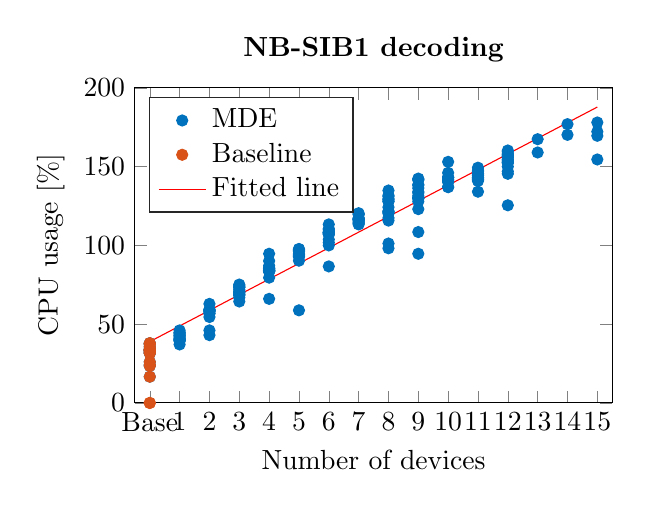
\begin{tikzpicture}

\begin{axis}[%
width=0.5\textwidth,
height=0.33\textwidth,
at={(0\textwidth,0\textwidth)},
scale only axis,
xmin=-0.5,
xmax=15.5,
xtick={0,1,2,3,4,5,6,7,8,9,10,11,12,13,14,15},
xticklabels={{Base},{1},{2},{3},{4},{5},{6},{7},{8},{9},{10},{11},{12},{13},{14},{15}},
xlabel={Number of devices},
ymin=0,
ymax=200,
ylabel={CPU usage [\%]},
axis background/.style={fill=white},
title style={font=\bfseries},
title={NB-SIB1 decoding},
legend style={at={(0.03,0.97)},anchor=north west,legend cell align=left,align=left,draw=white!15!black},
y tick label style={/pgf/number format/fixed}
]
\addplot [color=mycolor1,only marks,mark=*,mark options={solid}]
  table[row sep=crcr]{%
0	31.512\\
1	44.6925\\
4	66.062\\
5	96.97\\
6	86.666\\
7	114.3925\\
8	129.5425\\
11	143.0275\\
12	159.396\\
15	172.21\\
1	40.1475\\
2	58.186\\
3	70.4575\\
4	85.456\\
5	96.97\\
6	106.8175\\
8	117.4225\\
9	108.482\\
10	143.1775\\
11	145.454\\
12	157.578\\
0	16.665\\
1	39.39\\
2	46.064\\
3	73.4875\\
4	90.1525\\
5	92.728\\
6	110.605\\
7	116.362\\
8	127.876\\
9	131.4825\\
10	140.905\\
11	149.342\\
12	158.074\\
0	33.33\\
1	41.6625\\
2	62.8825\\
3	68.488\\
5	96.2125\\
6	108.3325\\
7	115.9075\\
8	124.24\\
9	123.028\\
10	141.6625\\
11	143.07\\
12	154.55\\
15	169.5875\\
0	31.815\\
1	42.42\\
2	56.8225\\
3	71.9725\\
5	58.788\\
6	108.3325\\
9	127.876\\
12	156.8225\\
13	158.986\\
0	23.4825\\
1	39.996\\
2	54.548\\
3	73.4875\\
4	84.0925\\
6	100\\
7	116.665\\
8	98.18\\
11	134.09\\
12	125.456\\
15	154.546\\
0	33.33\\
1	40.1475\\
4	84.85\\
7	116.665\\
8	121.21\\
9	129.694\\
11	147.722\\
12	155.76\\
3	74.548\\
4	87.1225\\
5	97.576\\
6	107.575\\
9	138.635\\
10	136.966\\
11	142.424\\
14	170.18\\
0	32.724\\
1	40.602\\
2	59.095\\
3	68.736\\
4	83.638\\
5	93.1825\\
6	113.332\\
8	115.756\\
9	130.14\\
11	146.9725\\
0	34.0875\\
2	43.034\\
3	69.7\\
6	103.7425\\
8	120.23\\
9	141.665\\
11	140.9075\\
0	33.936\\
2	58.3375\\
3	75.154\\
4	84.35\\
6	107.878\\
7	113.938\\
9	133.33\\
10	140.1475\\
11	145.7675\\
12	146.97\\
14	176.972\\
0	24.24\\
1	46.056\\
3	68.486\\
4	83.335\\
5	93.94\\
7	120.4525\\
8	101.21\\
9	130.104\\
10	153.0325\\
11	144.695\\
12	160.25\\
0	33.936\\
1	40.905\\
4	85.456\\
5	94.6975\\
6	108.3325\\
7	113.332\\
10	143.25\\
12	156.3975\\
15	178.03\\
0	33.33\\
1	37.1175\\
3	70.912\\
4	83.638\\
5	90.304\\
6	101.818\\
7	117.4225\\
8	129.088\\
9	138.18\\
0	37.875\\
1	43.026\\
2	59.398\\
4	85.6075\\
7	117.022\\
8	121.21\\
9	94.695\\
11	141.6625\\
12	152.73\\
13	167.4275\\
0	31.815\\
1	44.6925\\
4	84.244\\
6	107.272\\
7	116.665\\
8	131.0575\\
9	142.42\\
10	137.1175\\
12	150.0025\\
0	37.1175\\
1	43.935\\
2	58.792\\
3	64.395\\
4	79.5475\\
8	128.0275\\
9	130.3\\
10	146.06\\
12	152.275\\
0	35.6025\\
1	39.39\\
2	58.3375\\
3	73.4875\\
4	94.6975\\
7	119.695\\
8	131.815\\
9	136.36\\
10	143.026\\
12	145.456\\
0	37.875\\
1	43.026\\
2	56.8225\\
3	70.306\\
4	84.0925\\
5	93.94\\
6	109.8475\\
7	115.15\\
8	121.816\\
9	141.6625\\
11	141.6625\\
12	154.145\\
0	26.058\\
3	66.884\\
4	84.0925\\
5	97.7275\\
6	108.3325\\
7	119.695\\
8	134.845\\
9	134.0875\\
11	144.242\\
12	153.0325\\
};
\addlegendentry{MDE};

\addplot [color=mycolor2,only marks,mark=*,mark options={solid}]
  table[row sep=crcr]{%
0	31.512\\
0	0\\
0	16.665\\
0	33.33\\
0	31.815\\
0	23.4825\\
0	33.33\\
0	0\\
0	32.724\\
0	34.0875\\
0	33.936\\
0	24.24\\
0	33.936\\
0	33.33\\
0	37.875\\
0	31.815\\
0	37.1175\\
0	35.6025\\
0	37.875\\
0	26.058\\
};
\addlegendentry{Baseline};

\addplot [color=red,solid]
  table[row sep=crcr]{%
0	38.917490750578\\
0.015	39.0664021316152\\
0.03	39.2153135126525\\
0.045	39.3642248936897\\
0.06	39.513136274727\\
0.075	39.6620476557642\\
0.09	39.8109590368015\\
0.105	39.9598704178388\\
0.12	40.108781798876\\
0.135	40.2576931799133\\
0.15	40.4066045609505\\
0.165	40.5555159419878\\
0.18	40.704427323025\\
0.195	40.8533387040623\\
0.21	41.0022500850995\\
0.225	41.1511614661368\\
0.24	41.300072847174\\
0.255	41.4489842282113\\
0.27	41.5978956092485\\
0.285	41.7468069902858\\
0.3	41.895718371323\\
0.315	42.0446297523603\\
0.33	42.1935411333975\\
0.345	42.3424525144348\\
0.36	42.491363895472\\
0.375	42.6402752765093\\
0.39	42.7891866575465\\
0.405	42.9380980385838\\
0.42	43.087009419621\\
0.435	43.2359208006583\\
0.45	43.3848321816955\\
0.465	43.5337435627328\\
0.48	43.68265494377\\
0.495	43.8315663248073\\
0.51	43.9804777058445\\
0.525	44.1293890868818\\
0.54	44.278300467919\\
0.555	44.4272118489563\\
0.57	44.5761232299935\\
0.585	44.7250346110308\\
0.6	44.873945992068\\
0.615	45.0228573731053\\
0.63	45.1717687541425\\
0.645	45.3206801351798\\
0.66	45.4695915162171\\
0.675	45.6185028972543\\
0.69	45.7674142782916\\
0.705	45.9163256593288\\
0.72	46.0652370403661\\
0.735	46.2141484214033\\
0.75	46.3630598024406\\
0.765	46.5119711834778\\
0.78	46.6608825645151\\
0.795	46.8097939455523\\
0.81	46.9587053265896\\
0.825	47.1076167076268\\
0.84	47.2565280886641\\
0.855	47.4054394697013\\
0.87	47.5543508507386\\
0.885	47.7032622317758\\
0.9	47.8521736128131\\
0.915	48.0010849938503\\
0.93	48.1499963748876\\
0.945	48.2989077559248\\
0.96	48.4478191369621\\
0.975	48.5967305179993\\
0.99	48.7456418990366\\
1.005	48.8945532800738\\
1.02	49.0434646611111\\
1.035	49.1923760421483\\
1.05	49.3412874231856\\
1.065	49.4901988042228\\
1.08	49.6391101852601\\
1.095	49.7880215662973\\
1.11	49.9369329473346\\
1.125	50.0858443283718\\
1.14	50.2347557094091\\
1.155	50.3836670904463\\
1.17	50.5325784714836\\
1.185	50.6814898525208\\
1.2	50.8304012335581\\
1.215	50.9793126145953\\
1.23	51.1282239956326\\
1.245	51.2771353766698\\
1.26	51.4260467577071\\
1.275	51.5749581387444\\
1.29	51.7238695197816\\
1.305	51.8727809008189\\
1.32	52.0216922818561\\
1.335	52.1706036628934\\
1.35	52.3195150439306\\
1.365	52.4684264249679\\
1.38	52.6173378060051\\
1.395	52.7662491870424\\
1.41	52.9151605680796\\
1.425	53.0640719491169\\
1.44	53.2129833301541\\
1.455	53.3618947111914\\
1.47	53.5108060922286\\
1.485	53.6597174732659\\
1.5	53.8086288543031\\
1.515	53.9575402353404\\
1.53	54.1064516163776\\
1.545	54.2553629974149\\
1.56	54.4042743784521\\
1.575	54.5531857594894\\
1.59	54.7020971405266\\
1.605	54.8510085215639\\
1.62	54.9999199026011\\
1.635	55.1488312836384\\
1.65	55.2977426646756\\
1.665	55.4466540457129\\
1.68	55.5955654267501\\
1.695	55.7444768077874\\
1.71	55.8933881888246\\
1.725	56.0422995698619\\
1.74	56.1912109508991\\
1.755	56.3401223319364\\
1.77	56.4890337129737\\
1.785	56.6379450940109\\
1.8	56.7868564750481\\
1.815	56.9357678560854\\
1.83	57.0846792371227\\
1.845	57.2335906181599\\
1.86	57.3825019991972\\
1.875	57.5314133802344\\
1.89	57.6803247612717\\
1.905	57.8292361423089\\
1.92	57.9781475233462\\
1.935	58.1270589043834\\
1.95	58.2759702854207\\
1.965	58.4248816664579\\
1.98	58.5737930474952\\
1.995	58.7227044285324\\
2.01	58.8716158095697\\
2.025	59.0205271906069\\
2.04	59.1694385716442\\
2.055	59.3183499526814\\
2.07	59.4672613337187\\
2.085	59.6161727147559\\
2.1	59.7650840957932\\
2.115	59.9139954768304\\
2.13	60.0629068578677\\
2.145	60.2118182389049\\
2.16	60.3607296199422\\
2.175	60.5096410009794\\
2.19	60.6585523820167\\
2.205	60.8074637630539\\
2.22	60.9563751440912\\
2.235	61.1052865251284\\
2.25	61.2541979061657\\
2.265	61.4031092872029\\
2.28	61.5520206682402\\
2.295	61.7009320492774\\
2.31	61.8498434303147\\
2.325	61.9987548113519\\
2.34	62.1476661923892\\
2.355	62.2965775734264\\
2.37	62.4454889544637\\
2.385	62.594400335501\\
2.4	62.7433117165382\\
2.415	62.8922230975755\\
2.43	63.0411344786127\\
2.445	63.19004585965\\
2.46	63.3389572406872\\
2.475	63.4878686217245\\
2.49	63.6367800027617\\
2.505	63.785691383799\\
2.52	63.9346027648362\\
2.535	64.0835141458735\\
2.55	64.2324255269107\\
2.565	64.381336907948\\
2.58	64.5302482889852\\
2.595	64.6791596700225\\
2.61	64.8280710510597\\
2.625	64.976982432097\\
2.64	65.1258938131342\\
2.655	65.2748051941715\\
2.67	65.4237165752087\\
2.685	65.572627956246\\
2.7	65.7215393372832\\
2.715	65.8704507183205\\
2.73	66.0193620993577\\
2.745	66.168273480395\\
2.76	66.3171848614322\\
2.775	66.4660962424695\\
2.79	66.6150076235067\\
2.805	66.763919004544\\
2.82	66.9128303855812\\
2.835	67.0617417666185\\
2.85	67.2106531476557\\
2.865	67.359564528693\\
2.88	67.5084759097302\\
2.895	67.6573872907675\\
2.91	67.8062986718047\\
2.925	67.955210052842\\
2.94	68.1041214338792\\
2.955	68.2530328149165\\
2.97	68.4019441959537\\
2.985	68.550855576991\\
3	68.6997669580282\\
3.015	68.8486783390655\\
3.03	68.9975897201028\\
3.045	69.14650110114\\
3.06	69.2954124821773\\
3.075	69.4443238632145\\
3.09	69.5932352442518\\
3.105	69.742146625289\\
3.12	69.8910580063263\\
3.135	70.0399693873635\\
3.15	70.1888807684008\\
3.165	70.337792149438\\
3.18	70.4867035304753\\
3.195	70.6356149115125\\
3.21	70.7845262925498\\
3.225	70.933437673587\\
3.24	71.0823490546243\\
3.255	71.2312604356615\\
3.27	71.3801718166988\\
3.285	71.529083197736\\
3.3	71.6779945787733\\
3.315	71.8269059598105\\
3.33	71.9758173408478\\
3.345	72.124728721885\\
3.36	72.2736401029223\\
3.375	72.4225514839595\\
3.39	72.5714628649968\\
3.405	72.720374246034\\
3.42	72.8692856270713\\
3.435	73.0181970081085\\
3.45	73.1671083891458\\
3.465	73.316019770183\\
3.48	73.4649311512203\\
3.495	73.6138425322576\\
3.51	73.7627539132948\\
3.525	73.9116652943321\\
3.54	74.0605766753693\\
3.555	74.2094880564065\\
3.57	74.3583994374438\\
3.585	74.5073108184811\\
3.6	74.6562221995183\\
3.615	74.8051335805555\\
3.63	74.9540449615928\\
3.645	75.1029563426301\\
3.66	75.2518677236673\\
3.675	75.4007791047046\\
3.69	75.5496904857418\\
3.705	75.6986018667791\\
3.72	75.8475132478163\\
3.735	75.9964246288536\\
3.75	76.1453360098908\\
3.765	76.2942473909281\\
3.78	76.4431587719653\\
3.795	76.5920701530026\\
3.81	76.7409815340398\\
3.825	76.8898929150771\\
3.84	77.0388042961143\\
3.855	77.1877156771516\\
3.87	77.3366270581888\\
3.885	77.4855384392261\\
3.9	77.6344498202633\\
3.915	77.7833612013006\\
3.93	77.9322725823378\\
3.945	78.0811839633751\\
3.96	78.2300953444123\\
3.975	78.3790067254496\\
3.99	78.5279181064869\\
4.005	78.6768294875241\\
4.02	78.8257408685613\\
4.035	78.9746522495986\\
4.05	79.1235636306359\\
4.065	79.2724750116731\\
4.08	79.4213863927104\\
4.095	79.5702977737476\\
4.11	79.7192091547848\\
4.125	79.8681205358221\\
4.14	80.0170319168594\\
4.155	80.1659432978966\\
4.17	80.3148546789339\\
4.185	80.4637660599711\\
4.2	80.6126774410084\\
4.215	80.7615888220456\\
4.23	80.9105002030829\\
4.245	81.0594115841201\\
4.26	81.2083229651574\\
4.275	81.3572343461946\\
4.29	81.5061457272319\\
4.305	81.6550571082691\\
4.32	81.8039684893064\\
4.335	81.9528798703436\\
4.35	82.1017912513809\\
4.365	82.2507026324181\\
4.38	82.3996140134554\\
4.395	82.5485253944926\\
4.41	82.6974367755299\\
4.425	82.8463481565671\\
4.44	82.9952595376044\\
4.455	83.1441709186416\\
4.47	83.2930822996789\\
4.485	83.4419936807161\\
4.5	83.5909050617534\\
4.515	83.7398164427906\\
4.53	83.8887278238279\\
4.545	84.0376392048651\\
4.56	84.1865505859024\\
4.575	84.3354619669396\\
4.59	84.4843733479769\\
4.605	84.6332847290142\\
4.62	84.7821961100514\\
4.635	84.9311074910887\\
4.65	85.0800188721259\\
4.665	85.2289302531632\\
4.68	85.3778416342004\\
4.695	85.5267530152377\\
4.71	85.6756643962749\\
4.725	85.8245757773122\\
4.74	85.9734871583494\\
4.755	86.1223985393867\\
4.77	86.2713099204239\\
4.785	86.4202213014612\\
4.8	86.5691326824984\\
4.815	86.7180440635357\\
4.83	86.8669554445729\\
4.845	87.0158668256102\\
4.86	87.1647782066474\\
4.875	87.3136895876847\\
4.89	87.4626009687219\\
4.905	87.6115123497592\\
4.92	87.7604237307964\\
4.935	87.9093351118337\\
4.95	88.0582464928709\\
4.965	88.2071578739082\\
4.98	88.3560692549454\\
4.995	88.5049806359827\\
5.01	88.6538920170199\\
5.025	88.8028033980572\\
5.04	88.9517147790944\\
5.055	89.1006261601317\\
5.07	89.2495375411689\\
5.085	89.3984489222062\\
5.1	89.5473603032434\\
5.115	89.6962716842807\\
5.13	89.8451830653179\\
5.145	89.9940944463552\\
5.16	90.1430058273924\\
5.175	90.2919172084297\\
5.19	90.4408285894669\\
5.205	90.5897399705042\\
5.22	90.7386513515414\\
5.235	90.8875627325787\\
5.25	91.036474113616\\
5.265	91.1853854946532\\
5.28	91.3342968756905\\
5.295	91.4832082567277\\
5.31	91.632119637765\\
5.325	91.7810310188022\\
5.34	91.9299423998395\\
5.355	92.0788537808767\\
5.37	92.227765161914\\
5.385	92.3766765429512\\
5.4	92.5255879239885\\
5.415	92.6744993050257\\
5.43	92.823410686063\\
5.445	92.9723220671002\\
5.46	93.1212334481375\\
5.475	93.2701448291747\\
5.49	93.419056210212\\
5.505	93.5679675912492\\
5.52	93.7168789722865\\
5.535	93.8657903533237\\
5.55	94.014701734361\\
5.565	94.1636131153982\\
5.58	94.3125244964355\\
5.595	94.4614358774727\\
5.61	94.61034725851\\
5.625	94.7592586395472\\
5.64	94.9081700205845\\
5.655	95.0570814016217\\
5.67	95.205992782659\\
5.685	95.3549041636962\\
5.7	95.5038155447335\\
5.715	95.6527269257707\\
5.73	95.801638306808\\
5.745	95.9505496878453\\
5.76	96.0994610688825\\
5.775	96.2483724499197\\
5.79	96.397283830957\\
5.805	96.5461952119942\\
5.82	96.6951065930315\\
5.835	96.8440179740687\\
5.85	96.992929355106\\
5.865	97.1418407361433\\
5.88	97.2907521171805\\
5.895	97.4396634982178\\
5.91	97.588574879255\\
5.925	97.7374862602923\\
5.94	97.8863976413295\\
5.955	98.0353090223668\\
5.97	98.184220403404\\
5.985	98.3331317844413\\
6	98.4820431654785\\
6.015	98.6309545465158\\
6.03	98.779865927553\\
6.045	98.9287773085903\\
6.06	99.0776886896275\\
6.075	99.2266000706648\\
6.09	99.375511451702\\
6.105	99.5244228327393\\
6.12	99.6733342137765\\
6.135	99.8222455948138\\
6.15	99.971156975851\\
6.165	100.120068356888\\
6.18	100.268979737926\\
6.195	100.417891118963\\
6.21	100.5668025\\
6.225	100.715713881037\\
6.24	100.864625262075\\
6.255	101.013536643112\\
6.27	101.162448024149\\
6.285	101.311359405186\\
6.3	101.460270786224\\
6.315	101.609182167261\\
6.33	101.758093548298\\
6.345	101.907004929335\\
6.36	102.055916310373\\
6.375	102.20482769141\\
6.39	102.353739072447\\
6.405	102.502650453484\\
6.42	102.651561834522\\
6.435	102.800473215559\\
6.45	102.949384596596\\
6.465	103.098295977633\\
6.48	103.247207358671\\
6.495	103.396118739708\\
6.51	103.545030120745\\
6.525	103.693941501782\\
6.54	103.84285288282\\
6.555	103.991764263857\\
6.57	104.140675644894\\
6.585	104.289587025931\\
6.6	104.438498406969\\
6.615	104.587409788006\\
6.63	104.736321169043\\
6.645	104.88523255008\\
6.66	105.034143931118\\
6.675	105.183055312155\\
6.69	105.331966693192\\
6.705	105.480878074229\\
6.72	105.629789455267\\
6.735	105.778700836304\\
6.75	105.927612217341\\
6.765	106.076523598378\\
6.78	106.225434979416\\
6.795	106.374346360453\\
6.81	106.52325774149\\
6.825	106.672169122527\\
6.84	106.821080503565\\
6.855	106.969991884602\\
6.87	107.118903265639\\
6.885	107.267814646676\\
6.9	107.416726027714\\
6.915	107.565637408751\\
6.93	107.714548789788\\
6.945	107.863460170825\\
6.96	108.012371551863\\
6.975	108.1612829329\\
6.99	108.310194313937\\
7.005	108.459105694974\\
7.02	108.608017076012\\
7.035	108.756928457049\\
7.05	108.905839838086\\
7.065	109.054751219123\\
7.08	109.203662600161\\
7.095	109.352573981198\\
7.11	109.501485362235\\
7.125	109.650396743272\\
7.14	109.79930812431\\
7.155	109.948219505347\\
7.17	110.097130886384\\
7.185	110.246042267421\\
7.2	110.394953648459\\
7.215	110.543865029496\\
7.23	110.692776410533\\
7.245	110.84168779157\\
7.26	110.990599172608\\
7.275	111.139510553645\\
7.29	111.288421934682\\
7.305	111.437333315719\\
7.32	111.586244696757\\
7.335	111.735156077794\\
7.35	111.884067458831\\
7.365	112.032978839868\\
7.38	112.181890220906\\
7.395	112.330801601943\\
7.41	112.47971298298\\
7.425	112.628624364017\\
7.44	112.777535745055\\
7.455	112.926447126092\\
7.47	113.075358507129\\
7.485	113.224269888166\\
7.5	113.373181269204\\
7.515	113.522092650241\\
7.53	113.671004031278\\
7.545	113.819915412315\\
7.56	113.968826793353\\
7.575	114.11773817439\\
7.59	114.266649555427\\
7.605	114.415560936464\\
7.62	114.564472317502\\
7.635	114.713383698539\\
7.65	114.862295079576\\
7.665	115.011206460613\\
7.68	115.160117841651\\
7.695	115.309029222688\\
7.71	115.457940603725\\
7.725	115.606851984762\\
7.74	115.7557633658\\
7.755	115.904674746837\\
7.77	116.053586127874\\
7.785	116.202497508911\\
7.8	116.351408889949\\
7.815	116.500320270986\\
7.83	116.649231652023\\
7.845	116.79814303306\\
7.86	116.947054414098\\
7.875	117.095965795135\\
7.89	117.244877176172\\
7.905	117.393788557209\\
7.92	117.542699938247\\
7.935	117.691611319284\\
7.95	117.840522700321\\
7.965	117.989434081358\\
7.98	118.138345462396\\
7.995	118.287256843433\\
8.01	118.43616822447\\
8.025	118.585079605507\\
8.04	118.733990986545\\
8.055	118.882902367582\\
8.07	119.031813748619\\
8.085	119.180725129656\\
8.1	119.329636510694\\
8.115	119.478547891731\\
8.13	119.627459272768\\
8.145	119.776370653805\\
8.16	119.925282034843\\
8.175	120.07419341588\\
8.19	120.223104796917\\
8.205	120.372016177954\\
8.22	120.520927558992\\
8.235	120.669838940029\\
8.25	120.818750321066\\
8.265	120.967661702103\\
8.28	121.116573083141\\
8.295	121.265484464178\\
8.31	121.414395845215\\
8.325	121.563307226252\\
8.34	121.71221860729\\
8.355	121.861129988327\\
8.37	122.010041369364\\
8.385	122.158952750401\\
8.4	122.307864131439\\
8.415	122.456775512476\\
8.43	122.605686893513\\
8.445	122.75459827455\\
8.46	122.903509655588\\
8.475	123.052421036625\\
8.49	123.201332417662\\
8.505	123.350243798699\\
8.52	123.499155179737\\
8.535	123.648066560774\\
8.55	123.796977941811\\
8.565	123.945889322849\\
8.58	124.094800703886\\
8.595	124.243712084923\\
8.61	124.39262346596\\
8.625	124.541534846998\\
8.64	124.690446228035\\
8.655	124.839357609072\\
8.67	124.988268990109\\
8.685	125.137180371147\\
8.7	125.286091752184\\
8.715	125.435003133221\\
8.73	125.583914514258\\
8.745	125.732825895296\\
8.76	125.881737276333\\
8.775	126.03064865737\\
8.79	126.179560038407\\
8.805	126.328471419445\\
8.82	126.477382800482\\
8.835	126.626294181519\\
8.85	126.775205562556\\
8.865	126.924116943594\\
8.88	127.073028324631\\
8.895	127.221939705668\\
8.91	127.370851086705\\
8.925	127.519762467743\\
8.94	127.66867384878\\
8.955	127.817585229817\\
8.97	127.966496610854\\
8.985	128.115407991892\\
9	128.264319372929\\
9.015	128.413230753966\\
9.03	128.562142135003\\
9.045	128.711053516041\\
9.06	128.859964897078\\
9.075	129.008876278115\\
9.09	129.157787659152\\
9.105	129.30669904019\\
9.12	129.455610421227\\
9.135	129.604521802264\\
9.15	129.753433183301\\
9.165	129.902344564339\\
9.18	130.051255945376\\
9.195	130.200167326413\\
9.21	130.34907870745\\
9.225	130.497990088488\\
9.24	130.646901469525\\
9.255	130.795812850562\\
9.27	130.944724231599\\
9.285	131.093635612637\\
9.3	131.242546993674\\
9.315	131.391458374711\\
9.33	131.540369755748\\
9.345	131.689281136786\\
9.36	131.838192517823\\
9.375	131.98710389886\\
9.39	132.136015279897\\
9.405	132.284926660935\\
9.42	132.433838041972\\
9.435	132.582749423009\\
9.45	132.731660804046\\
9.465	132.880572185084\\
9.48	133.029483566121\\
9.495	133.178394947158\\
9.51	133.327306328195\\
9.525	133.476217709233\\
9.54	133.62512909027\\
9.555	133.774040471307\\
9.57	133.922951852344\\
9.585	134.071863233382\\
9.6	134.220774614419\\
9.615	134.369685995456\\
9.63	134.518597376493\\
9.645	134.667508757531\\
9.66	134.816420138568\\
9.675	134.965331519605\\
9.69	135.114242900642\\
9.705	135.26315428168\\
9.72	135.412065662717\\
9.735	135.560977043754\\
9.75	135.709888424791\\
9.765	135.858799805829\\
9.78	136.007711186866\\
9.795	136.156622567903\\
9.81	136.30553394894\\
9.825	136.454445329978\\
9.84	136.603356711015\\
9.855	136.752268092052\\
9.87	136.901179473089\\
9.885	137.050090854127\\
9.9	137.199002235164\\
9.915	137.347913616201\\
9.93	137.496824997238\\
9.945	137.645736378276\\
9.96	137.794647759313\\
9.975	137.94355914035\\
9.99	138.092470521387\\
10.005	138.241381902425\\
10.02	138.390293283462\\
10.035	138.539204664499\\
10.05	138.688116045536\\
10.065	138.837027426574\\
10.08	138.985938807611\\
10.095	139.134850188648\\
10.11	139.283761569685\\
10.125	139.432672950723\\
10.14	139.58158433176\\
10.155	139.730495712797\\
10.17	139.879407093834\\
10.185	140.028318474872\\
10.2	140.177229855909\\
10.215	140.326141236946\\
10.23	140.475052617983\\
10.245	140.623963999021\\
10.26	140.772875380058\\
10.275	140.921786761095\\
10.29	141.070698142132\\
10.305	141.21960952317\\
10.32	141.368520904207\\
10.335	141.517432285244\\
10.35	141.666343666281\\
10.365	141.815255047319\\
10.38	141.964166428356\\
10.395	142.113077809393\\
10.41	142.26198919043\\
10.425	142.410900571468\\
10.44	142.559811952505\\
10.455	142.708723333542\\
10.47	142.857634714579\\
10.485	143.006546095617\\
10.5	143.155457476654\\
10.515	143.304368857691\\
10.53	143.453280238728\\
10.545	143.602191619766\\
10.56	143.751103000803\\
10.575	143.90001438184\\
10.59	144.048925762877\\
10.605	144.197837143915\\
10.62	144.346748524952\\
10.635	144.495659905989\\
10.65	144.644571287026\\
10.665	144.793482668064\\
10.68	144.942394049101\\
10.695	145.091305430138\\
10.71	145.240216811175\\
10.725	145.389128192213\\
10.74	145.53803957325\\
10.755	145.686950954287\\
10.77	145.835862335324\\
10.785	145.984773716362\\
10.8	146.133685097399\\
10.815	146.282596478436\\
10.83	146.431507859473\\
10.845	146.580419240511\\
10.86	146.729330621548\\
10.875	146.878242002585\\
10.89	147.027153383622\\
10.905	147.17606476466\\
10.92	147.324976145697\\
10.935	147.473887526734\\
10.95	147.622798907771\\
10.965	147.771710288809\\
10.98	147.920621669846\\
10.995	148.069533050883\\
11.01	148.21844443192\\
11.025	148.367355812958\\
11.04	148.516267193995\\
11.055	148.665178575032\\
11.07	148.814089956069\\
11.085	148.963001337107\\
11.1	149.111912718144\\
11.115	149.260824099181\\
11.13	149.409735480218\\
11.145	149.558646861256\\
11.16	149.707558242293\\
11.175	149.85646962333\\
11.19	150.005381004367\\
11.205	150.154292385405\\
11.22	150.303203766442\\
11.235	150.452115147479\\
11.25	150.601026528516\\
11.265	150.749937909554\\
11.28	150.898849290591\\
11.295	151.047760671628\\
11.31	151.196672052665\\
11.325	151.345583433703\\
11.34	151.49449481474\\
11.355	151.643406195777\\
11.37	151.792317576815\\
11.385	151.941228957852\\
11.4	152.090140338889\\
11.415	152.239051719926\\
11.43	152.387963100964\\
11.445	152.536874482001\\
11.46	152.685785863038\\
11.475	152.834697244075\\
11.49	152.983608625113\\
11.505	153.13252000615\\
11.52	153.281431387187\\
11.535	153.430342768224\\
11.55	153.579254149262\\
11.565	153.728165530299\\
11.58	153.877076911336\\
11.595	154.025988292373\\
11.61	154.174899673411\\
11.625	154.323811054448\\
11.64	154.472722435485\\
11.655	154.621633816522\\
11.67	154.77054519756\\
11.685	154.919456578597\\
11.7	155.068367959634\\
11.715	155.217279340671\\
11.73	155.366190721709\\
11.745	155.515102102746\\
11.76	155.664013483783\\
11.775	155.81292486482\\
11.79	155.961836245858\\
11.805	156.110747626895\\
11.82	156.259659007932\\
11.835	156.408570388969\\
11.85	156.557481770007\\
11.865	156.706393151044\\
11.88	156.855304532081\\
11.895	157.004215913118\\
11.91	157.153127294156\\
11.925	157.302038675193\\
11.94	157.45095005623\\
11.955	157.599861437267\\
11.97	157.748772818305\\
11.985	157.897684199342\\
12	158.046595580379\\
12.015	158.195506961416\\
12.03	158.344418342454\\
12.045	158.493329723491\\
12.06	158.642241104528\\
12.075	158.791152485565\\
12.09	158.940063866603\\
12.105	159.08897524764\\
12.12	159.237886628677\\
12.135	159.386798009714\\
12.15	159.535709390752\\
12.165	159.684620771789\\
12.18	159.833532152826\\
12.195	159.982443533863\\
12.21	160.131354914901\\
12.225	160.280266295938\\
12.24	160.429177676975\\
12.255	160.578089058012\\
12.27	160.72700043905\\
12.285	160.875911820087\\
12.3	161.024823201124\\
12.315	161.173734582161\\
12.33	161.322645963199\\
12.345	161.471557344236\\
12.36	161.620468725273\\
12.375	161.76938010631\\
12.39	161.918291487348\\
12.405	162.067202868385\\
12.42	162.216114249422\\
12.435	162.365025630459\\
12.45	162.513937011497\\
12.465	162.662848392534\\
12.48	162.811759773571\\
12.495	162.960671154608\\
12.51	163.109582535646\\
12.525	163.258493916683\\
12.54	163.40740529772\\
12.555	163.556316678757\\
12.57	163.705228059795\\
12.585	163.854139440832\\
12.6	164.003050821869\\
12.615	164.151962202906\\
12.63	164.300873583944\\
12.645	164.449784964981\\
12.66	164.598696346018\\
12.675	164.747607727055\\
12.69	164.896519108093\\
12.705	165.04543048913\\
12.72	165.194341870167\\
12.735	165.343253251204\\
12.75	165.492164632242\\
12.765	165.641076013279\\
12.78	165.789987394316\\
12.795	165.938898775353\\
12.81	166.087810156391\\
12.825	166.236721537428\\
12.84	166.385632918465\\
12.855	166.534544299502\\
12.87	166.68345568054\\
12.885	166.832367061577\\
12.9	166.981278442614\\
12.915	167.130189823651\\
12.93	167.279101204689\\
12.945	167.428012585726\\
12.96	167.576923966763\\
12.975	167.7258353478\\
12.99	167.874746728838\\
13.005	168.023658109875\\
13.02	168.172569490912\\
13.035	168.321480871949\\
13.05	168.470392252987\\
13.065	168.619303634024\\
13.08	168.768215015061\\
13.095	168.917126396098\\
13.11	169.066037777136\\
13.125	169.214949158173\\
13.14	169.36386053921\\
13.155	169.512771920247\\
13.17	169.661683301285\\
13.185	169.810594682322\\
13.2	169.959506063359\\
13.215	170.108417444396\\
13.23	170.257328825434\\
13.245	170.406240206471\\
13.26	170.555151587508\\
13.275	170.704062968545\\
13.29	170.852974349583\\
13.305	171.00188573062\\
13.32	171.150797111657\\
13.335	171.299708492694\\
13.35	171.448619873732\\
13.365	171.597531254769\\
13.38	171.746442635806\\
13.395	171.895354016843\\
13.41	172.044265397881\\
13.425	172.193176778918\\
13.44	172.342088159955\\
13.455	172.490999540992\\
13.47	172.63991092203\\
13.485	172.788822303067\\
13.5	172.937733684104\\
13.515	173.086645065141\\
13.53	173.235556446179\\
13.545	173.384467827216\\
13.56	173.533379208253\\
13.575	173.68229058929\\
13.59	173.831201970328\\
13.605	173.980113351365\\
13.62	174.129024732402\\
13.635	174.277936113439\\
13.65	174.426847494477\\
13.665	174.575758875514\\
13.68	174.724670256551\\
13.695	174.873581637588\\
13.71	175.022493018626\\
13.725	175.171404399663\\
13.74	175.3203157807\\
13.755	175.469227161737\\
13.77	175.618138542775\\
13.785	175.767049923812\\
13.8	175.915961304849\\
13.815	176.064872685886\\
13.83	176.213784066924\\
13.845	176.362695447961\\
13.86	176.511606828998\\
13.875	176.660518210035\\
13.89	176.809429591073\\
13.905	176.95834097211\\
13.92	177.107252353147\\
13.935	177.256163734184\\
13.95	177.405075115222\\
13.965	177.553986496259\\
13.98	177.702897877296\\
13.995	177.851809258333\\
14.01	178.000720639371\\
14.025	178.149632020408\\
14.04	178.298543401445\\
14.055	178.447454782482\\
14.07	178.59636616352\\
14.085	178.745277544557\\
14.1	178.894188925594\\
14.115	179.043100306632\\
14.13	179.192011687669\\
14.145	179.340923068706\\
14.16	179.489834449743\\
14.175	179.63874583078\\
14.19	179.787657211818\\
14.205	179.936568592855\\
14.22	180.085479973892\\
14.235	180.23439135493\\
14.25	180.383302735967\\
14.265	180.532214117004\\
14.28	180.681125498041\\
14.295	180.830036879079\\
14.31	180.978948260116\\
14.325	181.127859641153\\
14.34	181.27677102219\\
14.355	181.425682403228\\
14.37	181.574593784265\\
14.385	181.723505165302\\
14.4	181.872416546339\\
14.415	182.021327927377\\
14.43	182.170239308414\\
14.445	182.319150689451\\
14.46	182.468062070488\\
14.475	182.616973451526\\
14.49	182.765884832563\\
14.505	182.9147962136\\
14.52	183.063707594637\\
14.535	183.212618975675\\
14.55	183.361530356712\\
14.565	183.510441737749\\
14.58	183.659353118786\\
14.595	183.808264499824\\
14.61	183.957175880861\\
14.625	184.106087261898\\
14.64	184.254998642935\\
14.655	184.403910023973\\
14.67	184.55282140501\\
14.685	184.701732786047\\
14.7	184.850644167084\\
14.715	184.999555548122\\
14.73	185.148466929159\\
14.745	185.297378310196\\
14.76	185.446289691233\\
14.775	185.595201072271\\
14.79	185.744112453308\\
14.805	185.893023834345\\
14.82	186.041935215382\\
14.835	186.19084659642\\
14.85	186.339757977457\\
14.865	186.488669358494\\
14.88	186.637580739531\\
14.895	186.786492120569\\
14.91	186.935403501606\\
14.925	187.084314882643\\
14.94	187.23322626368\\
14.955	187.382137644718\\
14.97	187.531049025755\\
14.985	187.679960406792\\
15	187.828871787829\\
};
\addlegendentry{Fitted line};

\end{axis}
\end{tikzpicture}%}
\caption{CPU usage for the NB-SIB1 step of the MDE for different number of devices and the baseline emulator. The fitted line is a linear approximation}
\label{fig:CPU_SIB1}
\end{figure}

The fitted line for the CPU usage is estimated to be:
\begin{equation}
CPU_{NB-SIB1} = 9.93 \cdot NoD + 38.92
\end{equation}

As seen on \autoref{fig:CPU_SIB1}, this step also have a higher CPU usage at higher number of devices. It is also seen that the CPU usage is raising above 100\%, but as there is multiple threads in work at this point, multiple kernels is also in use, where the CPU usage for each kernel is added together by the CPU stat tool. As mentioned a limit of seven CPU's are assumed, which gives a upper limit of 700\%. The reason for increase in CPU usage, compared to the previous steps, is that the individual devices is used at this point. In the previous two steps only the Co\_Phy was active.

\subsection{NB-SIB2}
The NB-SIB2 step is measured from the NB-SIB1 is decoded until NB-SIB2 is decoded, which gives the results seen on \autoref{fig:CPU_init}. 

\begin{figure}[H]
\tikzsetnextfilename{CPU_SIB2}
\centering
\resizebox{0.5\textwidth}{!}{
% This file was created by matlab2tikz.
%
%The latest updates can be retrieved from
%  http://www.mathworks.com/matlabcentral/fileexchange/22022-matlab2tikz-matlab2tikz
%where you can also make suggestions and rate matlab2tikz.
%
\definecolor{mycolor1}{rgb}{0.00000,0.44700,0.74100}%
\definecolor{mycolor2}{rgb}{0.85000,0.32500,0.09800}%
%
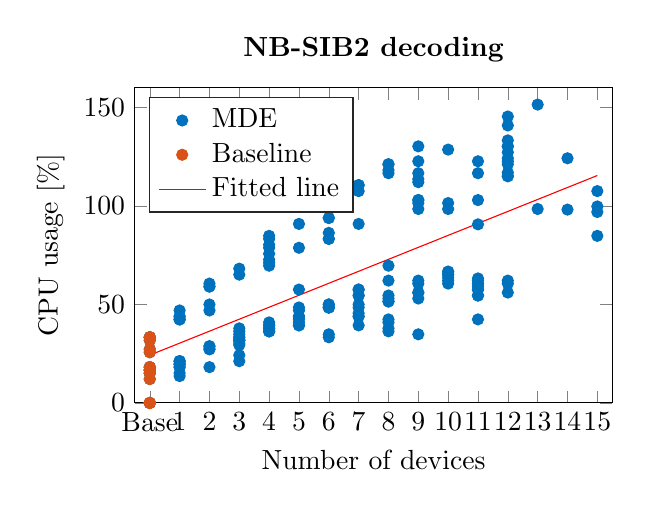
\begin{tikzpicture}

\begin{axis}[%
width=0.5\textwidth,
height=0.33\textwidth,
at={(0\textwidth,0\textwidth)},
scale only axis,
xmin=-0.5,
xmax=15.5,
xtick={0,1,2,3,4,5,6,7,8,9,10,11,12,13,14,15},
xticklabels={{Base},{1},{2},{3},{4},{5},{6},{7},{8},{9},{10},{11},{12},{13},{14},{15}},
xlabel={Number of devices},
ymin=0,
ymax=160,
ylabel={CPU usage [\%]},
axis background/.style={fill=white},
title style={font=\bfseries},
title={NB-SIB2 decoding},
legend style={at={(0.03,0.97)},anchor=north west,legend cell align=left,align=left,draw=white!15!black},
y tick label style={/pgf/number format/fixed}
]
\addplot [color=mycolor1,only marks,mark=*,mark options={solid}]
  table[row sep=crcr]{%
0	12.12\\
1	43.935\\
5	46.97\\
7	50\\
8	118.18\\
11	60.295\\
12	130.3\\
15	96.97\\
1	13.635\\
2	60.61\\
3	34.85\\
4	37.88\\
5	43.94\\
6	50\\
8	37.88\\
10	66.665\\
11	57.575\\
12	127.27\\
1	15.15\\
3	36.365\\
4	80.305\\
5	90.91\\
6	86.365\\
7	43.94\\
8	53.03\\
9	56.06\\
10	98.485\\
11	60.605\\
12	145.45\\
0	16.665\\
1	19.695\\
2	59.095\\
3	31.82\\
5	43.94\\
6	83.335\\
7	48.485\\
8	42.425\\
9	34.85\\
10	66.665\\
11	90.69\\
12	130.305\\
15	99.78\\
0	15.15\\
1	42.42\\
2	46.97\\
3	68.185\\
6	48.485\\
9	103.03\\
12	140.91\\
13	98.485\\
1	19.695\\
2	18.18\\
3	65.155\\
4	40.91\\
6	33.335\\
7	57.575\\
11	42.425\\
15	84.85\\
0	33.33\\
1	19.695\\
4	75.76\\
7	57.575\\
8	36.365\\
9	112.12\\
11	63.235\\
12	133.33\\
3	37.88\\
4	69.7\\
5	39.395\\
6	83.335\\
9	98.485\\
10	62.12\\
11	54.545\\
14	98.175\\
0	16.665\\
1	18.18\\
2	50\\
3	29.41\\
4	36.365\\
5	39.395\\
6	48.485\\
8	69.7\\
9	60.605\\
11	62.12\\
0	27.27\\
3	33.335\\
6	48.485\\
8	40.91\\
9	116.665\\
11	54.545\\
0	16.665\\
2	27.275\\
3	33.335\\
4	78.79\\
6	48.485\\
7	39.395\\
9	103.03\\
10	65.15\\
11	57.575\\
12	62.12\\
14	124.245\\
1	42.42\\
3	24.24\\
4	36.365\\
5	42.425\\
7	110.605\\
9	53.03\\
10	128.65\\
11	122.725\\
12	115.15\\
0	15.15\\
1	21.21\\
4	37.88\\
5	78.79\\
6	50\\
7	43.94\\
10	65.15\\
12	116.98\\
15	107.575\\
0	25.755\\
1	18.18\\
3	31.82\\
4	36.365\\
5	57.58\\
6	34.85\\
7	90.91\\
8	54.545\\
9	56.06\\
0	18.18\\
1	21.21\\
2	28.79\\
4	71.215\\
7	45.59\\
8	51.515\\
11	116.665\\
12	115.15\\
13	151.515\\
0	33.33\\
1	42.42\\
4	39.395\\
6	93.94\\
7	54.545\\
8	116.665\\
9	130.3\\
10	101.515\\
12	122.725\\
0	33.33\\
1	46.97\\
2	28.79\\
3	21.21\\
4	39.395\\
8	62.12\\
9	113.635\\
10	60.605\\
12	60.605\\
0	18.18\\
1	43.94\\
2	59.095\\
3	30.305\\
4	83.335\\
7	110.605\\
8	121.21\\
9	101.515\\
10	63.635\\
12	56.06\\
0	31.815\\
1	21.21\\
2	27.275\\
3	31.82\\
4	84.85\\
5	40.91\\
6	93.94\\
7	54.545\\
8	51.515\\
9	122.725\\
11	103.03\\
12	124.245\\
3	31.82\\
4	72.73\\
5	48.485\\
6	101.515\\
7	107.575\\
8	121.21\\
9	62.12\\
11	59.09\\
12	121.21\\
};
\addlegendentry{MDE};

\addplot [color=mycolor2,only marks,mark=*,mark options={solid}]
  table[row sep=crcr]{%
0	12.12\\
0	0\\
0	0\\
0	16.665\\
0	15.15\\
0	0\\
0	33.33\\
0	0\\
0	16.665\\
0	27.27\\
0	16.665\\
0	0\\
0	15.15\\
0	25.755\\
0	18.18\\
0	33.33\\
0	33.33\\
0	18.18\\
0	31.815\\
0	0\\
};
\addlegendentry{Baseline};

\addplot [color=red,solid]
  table[row sep=crcr]{%
0	24.2822432698915\\
0.015	24.3734563678329\\
0.03	24.4646694657743\\
0.045	24.5558825637157\\
0.06	24.6470956616571\\
0.075	24.7383087595984\\
0.09	24.8295218575398\\
0.105	24.9207349554812\\
0.12	25.0119480534226\\
0.135	25.103161151364\\
0.15	25.1943742493053\\
0.165	25.2855873472467\\
0.18	25.3768004451881\\
0.195	25.4680135431295\\
0.21	25.5592266410708\\
0.225	25.6504397390122\\
0.24	25.7416528369536\\
0.255	25.832865934895\\
0.27	25.9240790328364\\
0.285	26.0152921307777\\
0.3	26.1065052287191\\
0.315	26.1977183266605\\
0.33	26.2889314246019\\
0.345	26.3801445225433\\
0.36	26.4713576204846\\
0.375	26.562570718426\\
0.39	26.6537838163674\\
0.405	26.7449969143088\\
0.42	26.8362100122501\\
0.435	26.9274231101915\\
0.45	27.0186362081329\\
0.465	27.1098493060743\\
0.48	27.2010624040157\\
0.495	27.292275501957\\
0.51	27.3834885998984\\
0.525	27.4747016978398\\
0.54	27.5659147957812\\
0.555	27.6571278937226\\
0.57	27.7483409916639\\
0.585	27.8395540896053\\
0.6	27.9307671875467\\
0.615	28.0219802854881\\
0.63	28.1131933834294\\
0.645	28.2044064813708\\
0.66	28.2956195793122\\
0.675	28.3868326772536\\
0.69	28.478045775195\\
0.705	28.5692588731363\\
0.72	28.6604719710777\\
0.735	28.7516850690191\\
0.75	28.8428981669605\\
0.765	28.9341112649019\\
0.78	29.0253243628432\\
0.795	29.1165374607846\\
0.81	29.207750558726\\
0.825	29.2989636566674\\
0.84	29.3901767546087\\
0.855	29.4813898525501\\
0.87	29.5726029504915\\
0.885	29.6638160484329\\
0.9	29.7550291463743\\
0.915	29.8462422443156\\
0.93	29.937455342257\\
0.945	30.0286684401984\\
0.96	30.1198815381398\\
0.975	30.2110946360812\\
0.99	30.3023077340225\\
1.005	30.3935208319639\\
1.02	30.4847339299053\\
1.035	30.5759470278467\\
1.05	30.667160125788\\
1.065	30.7583732237294\\
1.08	30.8495863216708\\
1.095	30.9407994196122\\
1.11	31.0320125175536\\
1.125	31.1232256154949\\
1.14	31.2144387134363\\
1.155	31.3056518113777\\
1.17	31.3968649093191\\
1.185	31.4880780072605\\
1.2	31.5792911052018\\
1.215	31.6705042031432\\
1.23	31.7617173010846\\
1.245	31.852930399026\\
1.26	31.9441434969673\\
1.275	32.0353565949087\\
1.29	32.1265696928501\\
1.305	32.2177827907915\\
1.32	32.3089958887329\\
1.335	32.4002089866742\\
1.35	32.4914220846156\\
1.365	32.582635182557\\
1.38	32.6738482804984\\
1.395	32.7650613784398\\
1.41	32.8562744763811\\
1.425	32.9474875743225\\
1.44	33.0387006722639\\
1.455	33.1299137702053\\
1.47	33.2211268681466\\
1.485	33.312339966088\\
1.5	33.4035530640294\\
1.515	33.4947661619708\\
1.53	33.5859792599122\\
1.545	33.6771923578535\\
1.56	33.7684054557949\\
1.575	33.8596185537363\\
1.59	33.9508316516777\\
1.605	34.0420447496191\\
1.62	34.1332578475604\\
1.635	34.2244709455018\\
1.65	34.3156840434432\\
1.665	34.4068971413846\\
1.68	34.4981102393259\\
1.695	34.5893233372673\\
1.71	34.6805364352087\\
1.725	34.7717495331501\\
1.74	34.8629626310915\\
1.755	34.9541757290328\\
1.77	35.0453888269742\\
1.785	35.1366019249156\\
1.8	35.227815022857\\
1.815	35.3190281207984\\
1.83	35.4102412187397\\
1.845	35.5014543166811\\
1.86	35.5926674146225\\
1.875	35.6838805125639\\
1.89	35.7750936105052\\
1.905	35.8663067084466\\
1.92	35.957519806388\\
1.935	36.0487329043294\\
1.95	36.1399460022708\\
1.965	36.2311591002121\\
1.98	36.3223721981535\\
1.995	36.4135852960949\\
2.01	36.5047983940363\\
2.025	36.5960114919777\\
2.04	36.687224589919\\
2.055	36.7784376878604\\
2.07	36.8696507858018\\
2.085	36.9608638837432\\
2.1	37.0520769816846\\
2.115	37.1432900796259\\
2.13	37.2345031775673\\
2.145	37.3257162755087\\
2.16	37.4169293734501\\
2.175	37.5081424713914\\
2.19	37.5993555693328\\
2.205	37.6905686672742\\
2.22	37.7817817652156\\
2.235	37.872994863157\\
2.25	37.9642079610983\\
2.265	38.0554210590397\\
2.28	38.1466341569811\\
2.295	38.2378472549225\\
2.31	38.3290603528638\\
2.325	38.4202734508052\\
2.34	38.5114865487466\\
2.355	38.602699646688\\
2.37	38.6939127446294\\
2.385	38.7851258425707\\
2.4	38.8763389405121\\
2.415	38.9675520384535\\
2.43	39.0587651363949\\
2.445	39.1499782343363\\
2.46	39.2411913322776\\
2.475	39.332404430219\\
2.49	39.4236175281604\\
2.505	39.5148306261018\\
2.52	39.6060437240431\\
2.535	39.6972568219845\\
2.55	39.7884699199259\\
2.565	39.8796830178673\\
2.58	39.9708961158087\\
2.595	40.06210921375\\
2.61	40.1533223116914\\
2.625	40.2445354096328\\
2.64	40.3357485075742\\
2.655	40.4269616055156\\
2.67	40.5181747034569\\
2.685	40.6093878013983\\
2.7	40.7006008993397\\
2.715	40.7918139972811\\
2.73	40.8830270952224\\
2.745	40.9742401931638\\
2.76	41.0654532911052\\
2.775	41.1566663890466\\
2.79	41.247879486988\\
2.805	41.3390925849293\\
2.82	41.4303056828707\\
2.835	41.5215187808121\\
2.85	41.6127318787535\\
2.865	41.7039449766949\\
2.88	41.7951580746362\\
2.895	41.8863711725776\\
2.91	41.977584270519\\
2.925	42.0687973684604\\
2.94	42.1600104664017\\
2.955	42.2512235643431\\
2.97	42.3424366622845\\
2.985	42.4336497602259\\
3	42.5248628581673\\
3.015	42.6160759561086\\
3.03	42.70728905405\\
3.045	42.7985021519914\\
3.06	42.8897152499328\\
3.075	42.9809283478742\\
3.09	43.0721414458155\\
3.105	43.1633545437569\\
3.12	43.2545676416983\\
3.135	43.3457807396397\\
3.15	43.436993837581\\
3.165	43.5282069355224\\
3.18	43.6194200334638\\
3.195	43.7106331314052\\
3.21	43.8018462293466\\
3.225	43.8930593272879\\
3.24	43.9842724252293\\
3.255	44.0754855231707\\
3.27	44.1666986211121\\
3.285	44.2579117190535\\
3.3	44.3491248169948\\
3.315	44.4403379149362\\
3.33	44.5315510128776\\
3.345	44.622764110819\\
3.36	44.7139772087603\\
3.375	44.8051903067017\\
3.39	44.8964034046431\\
3.405	44.9876165025845\\
3.42	45.0788296005259\\
3.435	45.1700426984672\\
3.45	45.2612557964086\\
3.465	45.35246889435\\
3.48	45.4436819922914\\
3.495	45.5348950902328\\
3.51	45.6261081881741\\
3.525	45.7173212861155\\
3.54	45.8085343840569\\
3.555	45.8997474819983\\
3.57	45.9909605799396\\
3.585	46.082173677881\\
3.6	46.1733867758224\\
3.615	46.2645998737638\\
3.63	46.3558129717052\\
3.645	46.4470260696465\\
3.66	46.5382391675879\\
3.675	46.6294522655293\\
3.69	46.7206653634707\\
3.705	46.8118784614121\\
3.72	46.9030915593534\\
3.735	46.9943046572948\\
3.75	47.0855177552362\\
3.765	47.1767308531776\\
3.78	47.2679439511189\\
3.795	47.3591570490603\\
3.81	47.4503701470017\\
3.825	47.5415832449431\\
3.84	47.6327963428845\\
3.855	47.7240094408258\\
3.87	47.8152225387672\\
3.885	47.9064356367086\\
3.9	47.99764873465\\
3.915	48.0888618325913\\
3.93	48.1800749305327\\
3.945	48.2712880284741\\
3.96	48.3625011264155\\
3.975	48.4537142243569\\
3.99	48.5449273222982\\
4.005	48.6361404202396\\
4.02	48.727353518181\\
4.035	48.8185666161224\\
4.05	48.9097797140638\\
4.065	49.0009928120051\\
4.08	49.0922059099465\\
4.095	49.1834190078879\\
4.11	49.2746321058293\\
4.125	49.3658452037707\\
4.14	49.457058301712\\
4.155	49.5482713996534\\
4.17	49.6394844975948\\
4.185	49.7306975955362\\
4.2	49.8219106934775\\
4.215	49.9131237914189\\
4.23	50.0043368893603\\
4.245	50.0955499873017\\
4.26	50.1867630852431\\
4.275	50.2779761831844\\
4.29	50.3691892811258\\
4.305	50.4604023790672\\
4.32	50.5516154770086\\
4.335	50.64282857495\\
4.35	50.7340416728913\\
4.365	50.8252547708327\\
4.38	50.9164678687741\\
4.395	51.0076809667155\\
4.41	51.0988940646568\\
4.425	51.1901071625982\\
4.44	51.2813202605396\\
4.455	51.372533358481\\
4.47	51.4637464564224\\
4.485	51.5549595543637\\
4.5	51.6461726523051\\
4.515	51.7373857502465\\
4.53	51.8285988481879\\
4.545	51.9198119461293\\
4.56	52.0110250440706\\
4.575	52.102238142012\\
4.59	52.1934512399534\\
4.605	52.2846643378948\\
4.62	52.3758774358361\\
4.635	52.4670905337775\\
4.65	52.5583036317189\\
4.665	52.6495167296603\\
4.68	52.7407298276017\\
4.695	52.831942925543\\
4.71	52.9231560234844\\
4.725	53.0143691214258\\
4.74	53.1055822193672\\
4.755	53.1967953173086\\
4.77	53.2880084152499\\
4.785	53.3792215131913\\
4.8	53.4704346111327\\
4.815	53.5616477090741\\
4.83	53.6528608070154\\
4.845	53.7440739049568\\
4.86	53.8352870028982\\
4.875	53.9265001008396\\
4.89	54.017713198781\\
4.905	54.1089262967223\\
4.92	54.2001393946637\\
4.935	54.2913524926051\\
4.95	54.3825655905465\\
4.965	54.4737786884879\\
4.98	54.5649917864292\\
4.995	54.6562048843706\\
5.01	54.747417982312\\
5.025	54.8386310802534\\
5.04	54.9298441781947\\
5.055	55.0210572761361\\
5.07	55.1122703740775\\
5.085	55.2034834720189\\
5.1	55.2946965699603\\
5.115	55.3859096679016\\
5.13	55.477122765843\\
5.145	55.5683358637844\\
5.16	55.6595489617258\\
5.175	55.7507620596672\\
5.19	55.8419751576085\\
5.205	55.9331882555499\\
5.22	56.0244013534913\\
5.235	56.1156144514327\\
5.25	56.206827549374\\
5.265	56.2980406473154\\
5.28	56.3892537452568\\
5.295	56.4804668431982\\
5.31	56.5716799411396\\
5.325	56.6628930390809\\
5.34	56.7541061370223\\
5.355	56.8453192349637\\
5.37	56.9365323329051\\
5.385	57.0277454308465\\
5.4	57.1189585287878\\
5.415	57.2101716267292\\
5.43	57.3013847246706\\
5.445	57.392597822612\\
5.46	57.4838109205533\\
5.475	57.5750240184947\\
5.49	57.6662371164361\\
5.505	57.7574502143775\\
5.52	57.8486633123189\\
5.535	57.9398764102602\\
5.55	58.0310895082016\\
5.565	58.122302606143\\
5.58	58.2135157040844\\
5.595	58.3047288020258\\
5.61	58.3959418999671\\
5.625	58.4871549979085\\
5.64	58.5783680958499\\
5.655	58.6695811937913\\
5.67	58.7607942917326\\
5.685	58.852007389674\\
5.7	58.9432204876154\\
5.715	59.0344335855568\\
5.73	59.1256466834982\\
5.745	59.2168597814395\\
5.76	59.3080728793809\\
5.775	59.3992859773223\\
5.79	59.4904990752637\\
5.805	59.581712173205\\
5.82	59.6729252711464\\
5.835	59.7641383690878\\
5.85	59.8553514670292\\
5.865	59.9465645649706\\
5.88	60.037777662912\\
5.895	60.1289907608533\\
5.91	60.2202038587947\\
5.925	60.3114169567361\\
5.94	60.4026300546775\\
5.955	60.4938431526188\\
5.97	60.5850562505602\\
5.985	60.6762693485016\\
6	60.767482446443\\
6.015	60.8586955443843\\
6.03	60.9499086423257\\
6.045	61.0411217402671\\
6.06	61.1323348382085\\
6.075	61.2235479361499\\
6.09	61.3147610340912\\
6.105	61.4059741320326\\
6.12	61.497187229974\\
6.135	61.5884003279154\\
6.15	61.6796134258568\\
6.165	61.7708265237981\\
6.18	61.8620396217395\\
6.195	61.9532527196809\\
6.21	62.0444658176223\\
6.225	62.1356789155636\\
6.24	62.226892013505\\
6.255	62.3181051114464\\
6.27	62.4093182093878\\
6.285	62.5005313073292\\
6.3	62.5917444052705\\
6.315	62.6829575032119\\
6.33	62.7741706011533\\
6.345	62.8653836990947\\
6.36	62.9565967970361\\
6.375	63.0478098949774\\
6.39	63.1390229929188\\
6.405	63.2302360908602\\
6.42	63.3214491888016\\
6.435	63.4126622867429\\
6.45	63.5038753846843\\
6.465	63.5950884826257\\
6.48	63.6863015805671\\
6.495	63.7775146785085\\
6.51	63.8687277764498\\
6.525	63.9599408743912\\
6.54	64.0511539723326\\
6.555	64.142367070274\\
6.57	64.2335801682154\\
6.585	64.3247932661567\\
6.6	64.4160063640981\\
6.615	64.5072194620395\\
6.63	64.5984325599809\\
6.645	64.6896456579222\\
6.66	64.7808587558636\\
6.675	64.872071853805\\
6.69	64.9632849517464\\
6.705	65.0544980496878\\
6.72	65.1457111476291\\
6.735	65.2369242455705\\
6.75	65.3281373435119\\
6.765	65.4193504414533\\
6.78	65.5105635393947\\
6.795	65.601776637336\\
6.81	65.6929897352774\\
6.825	65.7842028332188\\
6.84	65.8754159311602\\
6.855	65.9666290291016\\
6.87	66.0578421270429\\
6.885	66.1490552249843\\
6.9	66.2402683229257\\
6.915	66.3314814208671\\
6.93	66.4226945188084\\
6.945	66.5139076167498\\
6.96	66.6051207146912\\
6.975	66.6963338126326\\
6.99	66.787546910574\\
7.005	66.8787600085153\\
7.02	66.9699731064567\\
7.035	67.0611862043981\\
7.05	67.1523993023395\\
7.065	67.2436124002809\\
7.08	67.3348254982222\\
7.095	67.4260385961636\\
7.11	67.517251694105\\
7.125	67.6084647920464\\
7.14	67.6996778899877\\
7.155	67.7908909879291\\
7.17	67.8821040858705\\
7.185	67.9733171838119\\
7.2	68.0645302817533\\
7.215	68.1557433796946\\
7.23	68.246956477636\\
7.245	68.3381695755774\\
7.26	68.4293826735188\\
7.275	68.5205957714602\\
7.29	68.6118088694015\\
7.305	68.7030219673429\\
7.32	68.7942350652843\\
7.335	68.8854481632257\\
7.35	68.976661261167\\
7.365	69.0678743591084\\
7.38	69.1590874570498\\
7.395	69.2503005549912\\
7.41	69.3415136529326\\
7.425	69.4327267508739\\
7.44	69.5239398488153\\
7.455	69.6151529467567\\
7.47	69.7063660446981\\
7.485	69.7975791426394\\
7.5	69.8887922405808\\
7.515	69.9800053385222\\
7.53	70.0712184364636\\
7.545	70.162431534405\\
7.56	70.2536446323463\\
7.575	70.3448577302877\\
7.59	70.4360708282291\\
7.605	70.5272839261705\\
7.62	70.6184970241119\\
7.635	70.7097101220532\\
7.65	70.8009232199946\\
7.665	70.892136317936\\
7.68	70.9833494158774\\
7.695	71.0745625138187\\
7.71	71.1657756117601\\
7.725	71.2569887097015\\
7.74	71.3482018076429\\
7.755	71.4394149055843\\
7.77	71.5306280035256\\
7.785	71.621841101467\\
7.8	71.7130541994084\\
7.815	71.8042672973498\\
7.83	71.8954803952912\\
7.845	71.9866934932325\\
7.86	72.0779065911739\\
7.875	72.1691196891153\\
7.89	72.2603327870567\\
7.905	72.351545884998\\
7.92	72.4427589829394\\
7.935	72.5339720808808\\
7.95	72.6251851788222\\
7.965	72.7163982767636\\
7.98	72.8076113747049\\
7.995	72.8988244726463\\
8.01	72.9900375705877\\
8.025	73.0812506685291\\
8.04	73.1724637664705\\
8.055	73.2636768644118\\
8.07	73.3548899623532\\
8.085	73.4461030602946\\
8.1	73.537316158236\\
8.115	73.6285292561773\\
8.13	73.7197423541187\\
8.145	73.8109554520601\\
8.16	73.9021685500015\\
8.175	73.9933816479429\\
8.19	74.0845947458842\\
8.205	74.1758078438256\\
8.22	74.267020941767\\
8.235	74.3582340397084\\
8.25	74.4494471376498\\
8.265	74.5406602355911\\
8.28	74.6318733335325\\
8.295	74.7230864314739\\
8.31	74.8142995294153\\
8.325	74.9055126273566\\
8.34	74.996725725298\\
8.355	75.0879388232394\\
8.37	75.1791519211808\\
8.385	75.2703650191222\\
8.4	75.3615781170635\\
8.415	75.4527912150049\\
8.43	75.5440043129463\\
8.445	75.6352174108877\\
8.46	75.7264305088291\\
8.475	75.8176436067704\\
8.49	75.9088567047118\\
8.505	76.0000698026532\\
8.52	76.0912829005946\\
8.535	76.182495998536\\
8.55	76.2737090964773\\
8.565	76.3649221944187\\
8.58	76.4561352923601\\
8.595	76.5473483903015\\
8.61	76.6385614882428\\
8.625	76.7297745861842\\
8.64	76.8209876841256\\
8.655	76.912200782067\\
8.67	77.0034138800084\\
8.685	77.0946269779497\\
8.7	77.1858400758911\\
8.715	77.2770531738325\\
8.73	77.3682662717739\\
8.745	77.4594793697152\\
8.76	77.5506924676566\\
8.775	77.641905565598\\
8.79	77.7331186635394\\
8.805	77.8243317614808\\
8.82	77.9155448594221\\
8.835	78.0067579573635\\
8.85	78.0979710553049\\
8.865	78.1891841532463\\
8.88	78.2803972511877\\
8.895	78.371610349129\\
8.91	78.4628234470704\\
8.925	78.5540365450118\\
8.94	78.6452496429532\\
8.955	78.7364627408946\\
8.97	78.8276758388359\\
8.985	78.9188889367773\\
9	79.0101020347187\\
9.015	79.1013151326601\\
9.03	79.1925282306014\\
9.045	79.2837413285428\\
9.06	79.3749544264842\\
9.075	79.4661675244256\\
9.09	79.5573806223669\\
9.105	79.6485937203083\\
9.12	79.7398068182497\\
9.135	79.8310199161911\\
9.15	79.9222330141325\\
9.165	80.0134461120739\\
9.18	80.1046592100152\\
9.195	80.1958723079566\\
9.21	80.287085405898\\
9.225	80.3782985038394\\
9.24	80.4695116017807\\
9.255	80.5607246997221\\
9.27	80.6519377976635\\
9.285	80.7431508956049\\
9.3	80.8343639935462\\
9.315	80.9255770914876\\
9.33	81.016790189429\\
9.345	81.1080032873704\\
9.36	81.1992163853118\\
9.375	81.2904294832531\\
9.39	81.3816425811945\\
9.405	81.4728556791359\\
9.42	81.5640687770773\\
9.435	81.6552818750187\\
9.45	81.74649497296\\
9.465	81.8377080709014\\
9.48	81.9289211688428\\
9.495	82.0201342667842\\
9.51	82.1113473647256\\
9.525	82.2025604626669\\
9.54	82.2937735606083\\
9.555	82.3849866585497\\
9.57	82.4761997564911\\
9.585	82.5674128544324\\
9.6	82.6586259523738\\
9.615	82.7498390503152\\
9.63	82.8410521482566\\
9.645	82.932265246198\\
9.66	83.0234783441393\\
9.675	83.1146914420807\\
9.69	83.2059045400221\\
9.705	83.2971176379635\\
9.72	83.3883307359048\\
9.735	83.4795438338462\\
9.75	83.5707569317876\\
9.765	83.661970029729\\
9.78	83.7531831276704\\
9.795	83.8443962256117\\
9.81	83.9356093235531\\
9.825	84.0268224214945\\
9.84	84.1180355194359\\
9.855	84.2092486173773\\
9.87	84.3004617153186\\
9.885	84.39167481326\\
9.9	84.4828879112014\\
9.915	84.5741010091428\\
9.93	84.6653141070842\\
9.945	84.7565272050255\\
9.96	84.8477403029669\\
9.975	84.9389534009083\\
9.99	85.0301664988497\\
10.005	85.121379596791\\
10.02	85.2125926947324\\
10.035	85.3038057926738\\
10.05	85.3950188906152\\
10.065	85.4862319885566\\
10.08	85.5774450864979\\
10.095	85.6686581844393\\
10.11	85.7598712823807\\
10.125	85.8510843803221\\
10.14	85.9422974782634\\
10.155	86.0335105762048\\
10.17	86.1247236741462\\
10.185	86.2159367720876\\
10.2	86.307149870029\\
10.215	86.3983629679703\\
10.23	86.4895760659117\\
10.245	86.5807891638531\\
10.26	86.6720022617945\\
10.275	86.7632153597359\\
10.29	86.8544284576772\\
10.305	86.9456415556186\\
10.32	87.03685465356\\
10.335	87.1280677515014\\
10.35	87.2192808494428\\
10.365	87.3104939473841\\
10.38	87.4017070453255\\
10.395	87.4929201432669\\
10.41	87.5841332412083\\
10.425	87.6753463391496\\
10.44	87.766559437091\\
10.455	87.8577725350324\\
10.47	87.9489856329738\\
10.485	88.0401987309152\\
10.5	88.1314118288565\\
10.515	88.2226249267979\\
10.53	88.3138380247393\\
10.545	88.4050511226807\\
10.56	88.4962642206221\\
10.575	88.5874773185634\\
10.59	88.6786904165048\\
10.605	88.7699035144462\\
10.62	88.8611166123876\\
10.635	88.952329710329\\
10.65	89.0435428082703\\
10.665	89.1347559062117\\
10.68	89.2259690041531\\
10.695	89.3171821020945\\
10.71	89.4083952000358\\
10.725	89.4996082979772\\
10.74	89.5908213959186\\
10.755	89.68203449386\\
10.77	89.7732475918014\\
10.785	89.8644606897427\\
10.8	89.9556737876841\\
10.815	90.0468868856255\\
10.83	90.1380999835669\\
10.845	90.2293130815082\\
10.86	90.3205261794496\\
10.875	90.411739277391\\
10.89	90.5029523753324\\
10.905	90.5941654732738\\
10.92	90.6853785712151\\
10.935	90.7765916691565\\
10.95	90.8678047670979\\
10.965	90.9590178650393\\
10.98	91.0502309629807\\
10.995	91.141444060922\\
11.01	91.2326571588634\\
11.025	91.3238702568048\\
11.04	91.4150833547462\\
11.055	91.5062964526876\\
11.07	91.5975095506289\\
11.085	91.6887226485703\\
11.1	91.7799357465117\\
11.115	91.8711488444531\\
11.13	91.9623619423944\\
11.145	92.0535750403358\\
11.16	92.1447881382772\\
11.175	92.2360012362186\\
11.19	92.32721433416\\
11.205	92.4184274321013\\
11.22	92.5096405300427\\
11.235	92.6008536279841\\
11.25	92.6920667259255\\
11.265	92.7832798238668\\
11.28	92.8744929218082\\
11.295	92.9657060197496\\
11.31	93.056919117691\\
11.325	93.1481322156324\\
11.34	93.2393453135737\\
11.355	93.3305584115151\\
11.37	93.4217715094565\\
11.385	93.5129846073979\\
11.4	93.6041977053393\\
11.415	93.6954108032806\\
11.43	93.786623901222\\
11.445	93.8778369991634\\
11.46	93.9690500971048\\
11.475	94.0602631950461\\
11.49	94.1514762929875\\
11.505	94.2426893909289\\
11.52	94.3339024888703\\
11.535	94.4251155868117\\
11.55	94.516328684753\\
11.565	94.6075417826944\\
11.58	94.6987548806358\\
11.595	94.7899679785772\\
11.61	94.8811810765186\\
11.625	94.9723941744599\\
11.64	95.0636072724013\\
11.655	95.1548203703427\\
11.67	95.2460334682841\\
11.685	95.3372465662254\\
11.7	95.4284596641668\\
11.715	95.5196727621082\\
11.73	95.6108858600496\\
11.745	95.702098957991\\
11.76	95.7933120559323\\
11.775	95.8845251538737\\
11.79	95.9757382518151\\
11.805	96.0669513497565\\
11.82	96.1581644476979\\
11.835	96.2493775456392\\
11.85	96.3405906435806\\
11.865	96.431803741522\\
11.88	96.5230168394634\\
11.895	96.6142299374047\\
11.91	96.7054430353461\\
11.925	96.7966561332875\\
11.94	96.8878692312289\\
11.955	96.9790823291703\\
11.97	97.0702954271116\\
11.985	97.161508525053\\
12	97.2527216229944\\
12.015	97.3439347209358\\
12.03	97.4351478188772\\
12.045	97.5263609168185\\
12.06	97.6175740147599\\
12.075	97.7087871127013\\
12.09	97.8000002106427\\
12.105	97.8912133085841\\
12.12	97.9824264065254\\
12.135	98.0736395044668\\
12.15	98.1648526024082\\
12.165	98.2560657003496\\
12.18	98.3472787982909\\
12.195	98.4384918962323\\
12.21	98.5297049941737\\
12.225	98.6209180921151\\
12.24	98.7121311900565\\
12.255	98.8033442879978\\
12.27	98.8945573859392\\
12.285	98.9857704838806\\
12.3	99.076983581822\\
12.315	99.1681966797633\\
12.33	99.2594097777047\\
12.345	99.3506228756461\\
12.36	99.4418359735875\\
12.375	99.5330490715289\\
12.39	99.6242621694702\\
12.405	99.7154752674116\\
12.42	99.806688365353\\
12.435	99.8979014632944\\
12.45	99.9891145612358\\
12.465	100.080327659177\\
12.48	100.171540757119\\
12.495	100.26275385506\\
12.51	100.353966953001\\
12.525	100.445180050943\\
12.54	100.536393148884\\
12.555	100.627606246825\\
12.57	100.718819344767\\
12.585	100.810032442708\\
12.6	100.90124554065\\
12.615	100.992458638591\\
12.63	101.083671736532\\
12.645	101.174884834474\\
12.66	101.266097932415\\
12.675	101.357311030356\\
12.69	101.448524128298\\
12.705	101.539737226239\\
12.72	101.630950324181\\
12.735	101.722163422122\\
12.75	101.813376520063\\
12.765	101.904589618005\\
12.78	101.995802715946\\
12.795	102.087015813887\\
12.81	102.178228911829\\
12.825	102.26944200977\\
12.84	102.360655107712\\
12.855	102.451868205653\\
12.87	102.543081303594\\
12.885	102.634294401536\\
12.9	102.725507499477\\
12.915	102.816720597418\\
12.93	102.90793369536\\
12.945	102.999146793301\\
12.96	103.090359891243\\
12.975	103.181572989184\\
12.99	103.272786087125\\
13.005	103.363999185067\\
13.02	103.455212283008\\
13.035	103.54642538095\\
13.05	103.637638478891\\
13.065	103.728851576832\\
13.08	103.820064674774\\
13.095	103.911277772715\\
13.11	104.002490870656\\
13.125	104.093703968598\\
13.14	104.184917066539\\
13.155	104.276130164481\\
13.17	104.367343262422\\
13.185	104.458556360363\\
13.2	104.549769458305\\
13.215	104.640982556246\\
13.23	104.732195654187\\
13.245	104.823408752129\\
13.26	104.91462185007\\
13.275	105.005834948012\\
13.29	105.097048045953\\
13.305	105.188261143894\\
13.32	105.279474241836\\
13.335	105.370687339777\\
13.35	105.461900437718\\
13.365	105.55311353566\\
13.38	105.644326633601\\
13.395	105.735539731543\\
13.41	105.826752829484\\
13.425	105.917965927425\\
13.44	106.009179025367\\
13.455	106.100392123308\\
13.47	106.191605221249\\
13.485	106.282818319191\\
13.5	106.374031417132\\
13.515	106.465244515074\\
13.53	106.556457613015\\
13.545	106.647670710956\\
13.56	106.738883808898\\
13.575	106.830096906839\\
13.59	106.921310004781\\
13.605	107.012523102722\\
13.62	107.103736200663\\
13.635	107.194949298605\\
13.65	107.286162396546\\
13.665	107.377375494487\\
13.68	107.468588592429\\
13.695	107.55980169037\\
13.71	107.651014788312\\
13.725	107.742227886253\\
13.74	107.833440984194\\
13.755	107.924654082136\\
13.77	108.015867180077\\
13.785	108.107080278018\\
13.8	108.19829337596\\
13.815	108.289506473901\\
13.83	108.380719571843\\
13.845	108.471932669784\\
13.86	108.563145767725\\
13.875	108.654358865667\\
13.89	108.745571963608\\
13.905	108.836785061549\\
13.92	108.927998159491\\
13.935	109.019211257432\\
13.95	109.110424355374\\
13.965	109.201637453315\\
13.98	109.292850551256\\
13.995	109.384063649198\\
14.01	109.475276747139\\
14.025	109.566489845081\\
14.04	109.657702943022\\
14.055	109.748916040963\\
14.07	109.840129138905\\
14.085	109.931342236846\\
14.1	110.022555334787\\
14.115	110.113768432729\\
14.13	110.20498153067\\
14.145	110.296194628612\\
14.16	110.387407726553\\
14.175	110.478620824494\\
14.19	110.569833922436\\
14.205	110.661047020377\\
14.22	110.752260118318\\
14.235	110.84347321626\\
14.25	110.934686314201\\
14.265	111.025899412143\\
14.28	111.117112510084\\
14.295	111.208325608025\\
14.31	111.299538705967\\
14.325	111.390751803908\\
14.34	111.481964901849\\
14.355	111.573177999791\\
14.37	111.664391097732\\
14.385	111.755604195674\\
14.4	111.846817293615\\
14.415	111.938030391556\\
14.43	112.029243489498\\
14.445	112.120456587439\\
14.46	112.21166968538\\
14.475	112.302882783322\\
14.49	112.394095881263\\
14.505	112.485308979205\\
14.52	112.576522077146\\
14.535	112.667735175087\\
14.55	112.758948273029\\
14.565	112.85016137097\\
14.58	112.941374468912\\
14.595	113.032587566853\\
14.61	113.123800664794\\
14.625	113.215013762736\\
14.64	113.306226860677\\
14.655	113.397439958618\\
14.67	113.48865305656\\
14.685	113.579866154501\\
14.7	113.671079252443\\
14.715	113.762292350384\\
14.73	113.853505448325\\
14.745	113.944718546267\\
14.76	114.035931644208\\
14.775	114.127144742149\\
14.79	114.218357840091\\
14.805	114.309570938032\\
14.82	114.400784035974\\
14.835	114.491997133915\\
14.85	114.583210231856\\
14.865	114.674423329798\\
14.88	114.765636427739\\
14.895	114.85684952568\\
14.91	114.948062623622\\
14.925	115.039275721563\\
14.94	115.130488819505\\
14.955	115.221701917446\\
14.97	115.312915015387\\
14.985	115.404128113329\\
15	115.49534121127\\
};
\addlegendentry{Fitted line};

\end{axis}
\end{tikzpicture}%}
\caption{CPU usage for the NB-SIB2 step of the MDE for different number of devices and the baseline emulator. The fitted line is a linear approximation}
\label{fig:CPU_SIB2}
\end{figure}

The fitted line for the CPU usage is estimated to be:
\begin{equation}
CPU_{NB-SIB2} = 6.08 \cdot NoD + 24.28
\end{equation}

As seen on \autoref{fig:CPU_SIB2}, the results show the same problems as seen for the NB-SIB1 step. An interesting tendency for the NB-SIB2 step, is that it looks to have two tendencies, one above the red fitting line and one below. This could be explained by the fact, that the NB-SIB2 step contains two parts, which is looking for the NB-SIB2 message and then decode it. As only the later half is the CPU heavy and the time used is so small compared to the sample rate (four samples at max), this can give some very spread results. 



\subsection{NPRACH}
The NPRACH step is measured from the decoding of NB-SIB2 is done until the msg1 is delivered to the transmit buffer, which has an average CPU usage as seen on \autoref{fig:CPU_init}.

\begin{figure}[H]
\tikzsetnextfilename{CPU_NPRACH}
\centering
\resizebox{0.5\textwidth}{!}{
% This file was created by matlab2tikz.
%
%The latest updates can be retrieved from
%  http://www.mathworks.com/matlabcentral/fileexchange/22022-matlab2tikz-matlab2tikz
%where you can also make suggestions and rate matlab2tikz.
%
\definecolor{mycolor1}{rgb}{0.00000,0.44700,0.74100}%
\definecolor{mycolor2}{rgb}{0.85000,0.32500,0.09800}%
%
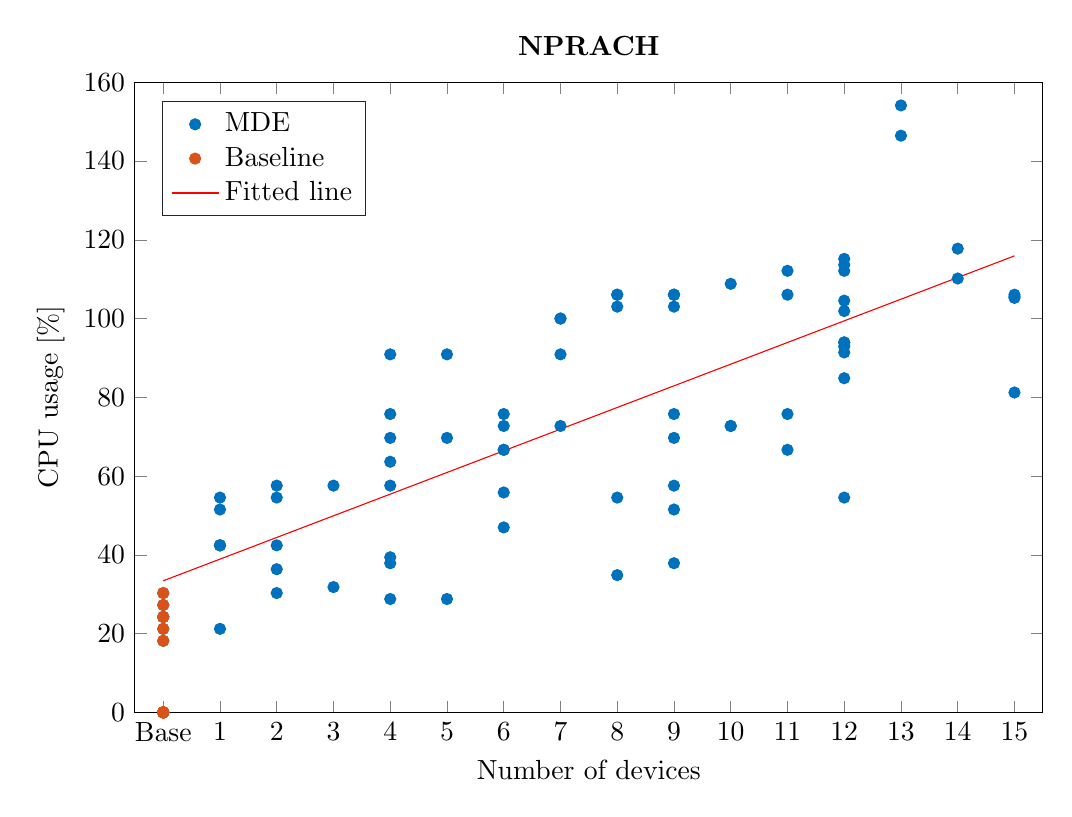
\begin{tikzpicture}

\begin{axis}[%
width=0.951\textwidth,
height=0.66\textwidth,
at={(0\textwidth,0\textwidth)},
scale only axis,
xmin=-0.5,
xmax=15.5,
xtick={0,1,2,3,4,5,6,7,8,9,10,11,12,13,14,15},
xticklabels={{Base},{1},{2},{3},{4},{5},{6},{7},{8},{9},{10},{11},{12},{13},{14},{15}},
xlabel={Number of devices},
ymin=0,
ymax=160,
ylabel={CPU usage [\%]},
axis background/.style={fill=white},
title style={font=\bfseries},
title={NPRACH},
legend style={at={(0.03,0.97)},anchor=north west,legend cell align=left,align=left,draw=white!15!black},
y tick label style={/pgf/number format/fixed}
]
\addplot [color=mycolor1,only marks,mark=*,mark options={solid}]
  table[row sep=crcr]{%
0	24.24\\
1	42.42\\
8	106.06\\
12	101.915\\
15	105.55375\\
2	30.305\\
12	115.15\\
4	69.7\\
5	90.91\\
6	66.67\\
10	72.73\\
12	113.635\\
2	54.55\\
6	66.67\\
11	66.67\\
12	54.545\\
15	81.223125\\
1	42.42\\
2	36.36\\
3	31.82\\
9	51.515\\
12	92.915\\
13	146.438571428571\\
3	57.58\\
15	106.061428571429\\
0	30.3\\
4	37.88\\
9	103.03\\
12	104.545\\
4	28.79\\
6	72.73\\
9	69.7\\
14	117.75\\
2	42.42\\
8	34.85\\
0	21.21\\
9	106.06\\
4	39.395\\
9	75.76\\
14	110.168\\
1	21.21\\
7	100\\
10	108.82\\
11	112.12\\
12	84.85\\
5	69.7\\
15	105.246875\\
0	18.18\\
5	28.79\\
7	72.73\\
4	57.58\\
11	106.06\\
12	91.4\\
13	154.115\\
1	42.42\\
6	46.97\\
8	106.06\\
9	57.575\\
10	72.73\\
12	112.12\\
0	27.27\\
1	54.55\\
9	106.06\\
1	51.52\\
2	57.58\\
4	75.76\\
7	100\\
8	54.545\\
9	37.88\\
0	24.24\\
4	90.91\\
6	75.76\\
9	106.06\\
11	75.76\\
12	93.94\\
4	63.64\\
6	55.8414285714286\\
7	90.91\\
8	103.03\\
12	93.94\\
};
\addlegendentry{MDE};

\addplot [color=mycolor2,only marks,mark=*,mark options={solid}]
  table[row sep=crcr]{%
0	24.24\\
0	0\\
0	0\\
0	0\\
0	0\\
0	0\\
0	30.3\\
0	0\\
0	0\\
0	21.21\\
0	0\\
0	0\\
0	0\\
0	18.18\\
0	0\\
0	0\\
0	27.27\\
0	0\\
0	24.24\\
0	0\\
};
\addlegendentry{Baseline};

\addplot [color=red,solid]
  table[row sep=crcr]{%
0	33.4187885533414\\
0.015	33.5012889477918\\
0.03	33.5837893422423\\
0.045	33.6662897366928\\
0.06	33.7487901311432\\
0.075	33.8312905255937\\
0.09	33.9137909200441\\
0.105	33.9962913144946\\
0.12	34.078791708945\\
0.135	34.1612921033955\\
0.15	34.2437924978459\\
0.165	34.3262928922964\\
0.18	34.4087932867469\\
0.195	34.4912936811973\\
0.21	34.5737940756478\\
0.225	34.6562944700982\\
0.24	34.7387948645487\\
0.255	34.8212952589991\\
0.27	34.9037956534496\\
0.285	34.9862960479\\
0.3	35.0687964423505\\
0.315	35.151296836801\\
0.33	35.2337972312514\\
0.345	35.3162976257019\\
0.36	35.3987980201523\\
0.375	35.4812984146028\\
0.39	35.5637988090532\\
0.405	35.6462992035037\\
0.42	35.7287995979542\\
0.435	35.8112999924046\\
0.45	35.8938003868551\\
0.465	35.9763007813055\\
0.48	36.058801175756\\
0.495	36.1413015702064\\
0.51	36.2238019646569\\
0.525	36.3063023591073\\
0.54	36.3888027535578\\
0.555	36.4713031480083\\
0.57	36.5538035424587\\
0.585	36.6363039369092\\
0.6	36.7188043313596\\
0.615	36.8013047258101\\
0.63	36.8838051202605\\
0.645	36.966305514711\\
0.66	37.0488059091615\\
0.675	37.1313063036119\\
0.69	37.2138066980624\\
0.705	37.2963070925128\\
0.72	37.3788074869633\\
0.735	37.4613078814137\\
0.75	37.5438082758642\\
0.765	37.6263086703146\\
0.78	37.7088090647651\\
0.795	37.7913094592156\\
0.81	37.873809853666\\
0.825	37.9563102481165\\
0.84	38.0388106425669\\
0.855	38.1213110370174\\
0.87	38.2038114314678\\
0.885	38.2863118259183\\
0.9	38.3688122203687\\
0.915	38.4513126148192\\
0.93	38.5338130092697\\
0.945	38.6163134037201\\
0.96	38.6988137981706\\
0.975	38.781314192621\\
0.99	38.8638145870715\\
1.005	38.9463149815219\\
1.02	39.0288153759724\\
1.035	39.1113157704228\\
1.05	39.1938161648733\\
1.065	39.2763165593238\\
1.08	39.3588169537742\\
1.095	39.4413173482247\\
1.11	39.5238177426751\\
1.125	39.6063181371256\\
1.14	39.688818531576\\
1.155	39.7713189260265\\
1.17	39.853819320477\\
1.185	39.9363197149274\\
1.2	40.0188201093779\\
1.215	40.1013205038283\\
1.23	40.1838208982788\\
1.245	40.2663212927292\\
1.26	40.3488216871797\\
1.275	40.4313220816301\\
1.29	40.5138224760806\\
1.305	40.5963228705311\\
1.32	40.6788232649815\\
1.335	40.761323659432\\
1.35	40.8438240538824\\
1.365	40.9263244483329\\
1.38	41.0088248427833\\
1.395	41.0913252372338\\
1.41	41.1738256316843\\
1.425	41.2563260261347\\
1.44	41.3388264205852\\
1.455	41.4213268150356\\
1.47	41.5038272094861\\
1.485	41.5863276039365\\
1.5	41.668827998387\\
1.515	41.7513283928374\\
1.53	41.8338287872879\\
1.545	41.9163291817384\\
1.56	41.9988295761888\\
1.575	42.0813299706393\\
1.59	42.1638303650897\\
1.605	42.2463307595402\\
1.62	42.3288311539906\\
1.635	42.4113315484411\\
1.65	42.4938319428915\\
1.665	42.576332337342\\
1.68	42.6588327317925\\
1.695	42.7413331262429\\
1.71	42.8238335206934\\
1.725	42.9063339151438\\
1.74	42.9888343095943\\
1.755	43.0713347040447\\
1.77	43.1538350984952\\
1.785	43.2363354929456\\
1.8	43.3188358873961\\
1.815	43.4013362818466\\
1.83	43.483836676297\\
1.845	43.5663370707475\\
1.86	43.6488374651979\\
1.875	43.7313378596484\\
1.89	43.8138382540988\\
1.905	43.8963386485493\\
1.92	43.9788390429998\\
1.935	44.0613394374502\\
1.95	44.1438398319007\\
1.965	44.2263402263511\\
1.98	44.3088406208016\\
1.995	44.391341015252\\
2.01	44.4738414097025\\
2.025	44.556341804153\\
2.04	44.6388421986034\\
2.055	44.7213425930539\\
2.07	44.8038429875043\\
2.085	44.8863433819548\\
2.1	44.9688437764052\\
2.115	45.0513441708557\\
2.13	45.1338445653061\\
2.145	45.2163449597566\\
2.16	45.2988453542071\\
2.175	45.3813457486575\\
2.19	45.463846143108\\
2.205	45.5463465375584\\
2.22	45.6288469320089\\
2.235	45.7113473264593\\
2.25	45.7938477209098\\
2.265	45.8763481153602\\
2.28	45.9588485098107\\
2.295	46.0413489042612\\
2.31	46.1238492987116\\
2.325	46.2063496931621\\
2.34	46.2888500876125\\
2.355	46.371350482063\\
2.37	46.4538508765134\\
2.385	46.5363512709639\\
2.4	46.6188516654143\\
2.415	46.7013520598648\\
2.43	46.7838524543153\\
2.445	46.8663528487657\\
2.46	46.9488532432162\\
2.475	47.0313536376666\\
2.49	47.1138540321171\\
2.505	47.1963544265675\\
2.52	47.278854821018\\
2.535	47.3613552154685\\
2.55	47.4438556099189\\
2.565	47.5263560043694\\
2.58	47.6088563988198\\
2.595	47.6913567932703\\
2.61	47.7738571877207\\
2.625	47.8563575821712\\
2.64	47.9388579766216\\
2.655	48.0213583710721\\
2.67	48.1038587655226\\
2.685	48.186359159973\\
2.7	48.2688595544235\\
2.715	48.3513599488739\\
2.73	48.4338603433244\\
2.745	48.5163607377748\\
2.76	48.5988611322253\\
2.775	48.6813615266757\\
2.79	48.7638619211262\\
2.805	48.8463623155767\\
2.82	48.9288627100271\\
2.835	49.0113631044776\\
2.85	49.093863498928\\
2.865	49.1763638933785\\
2.88	49.2588642878289\\
2.895	49.3413646822794\\
2.91	49.4238650767299\\
2.925	49.5063654711803\\
2.94	49.5888658656308\\
2.955	49.6713662600812\\
2.97	49.7538666545317\\
2.985	49.8363670489821\\
3	49.9188674434326\\
3.015	50.001367837883\\
3.03	50.0838682323335\\
3.045	50.166368626784\\
3.06	50.2488690212344\\
3.075	50.3313694156849\\
3.09	50.4138698101353\\
3.105	50.4963702045858\\
3.12	50.5788705990362\\
3.135	50.6613709934867\\
3.15	50.7438713879371\\
3.165	50.8263717823876\\
3.18	50.9088721768381\\
3.195	50.9913725712885\\
3.21	51.073872965739\\
3.225	51.1563733601894\\
3.24	51.2388737546399\\
3.255	51.3213741490903\\
3.27	51.4038745435408\\
3.285	51.4863749379913\\
3.3	51.5688753324417\\
3.315	51.6513757268922\\
3.33	51.7338761213426\\
3.345	51.8163765157931\\
3.36	51.8988769102435\\
3.375	51.981377304694\\
3.39	52.0638776991444\\
3.405	52.1463780935949\\
3.42	52.2288784880454\\
3.435	52.3113788824958\\
3.45	52.3938792769463\\
3.465	52.4763796713967\\
3.48	52.5588800658472\\
3.495	52.6413804602976\\
3.51	52.7238808547481\\
3.525	52.8063812491986\\
3.54	52.888881643649\\
3.555	52.9713820380995\\
3.57	53.0538824325499\\
3.585	53.1363828270004\\
3.6	53.2188832214508\\
3.615	53.3013836159013\\
3.63	53.3838840103517\\
3.645	53.4663844048022\\
3.66	53.5488847992526\\
3.675	53.6313851937031\\
3.69	53.7138855881536\\
3.705	53.796385982604\\
3.72	53.8788863770545\\
3.735	53.9613867715049\\
3.75	54.0438871659554\\
3.765	54.1263875604058\\
3.78	54.2088879548563\\
3.795	54.2913883493068\\
3.81	54.3738887437572\\
3.825	54.4563891382077\\
3.84	54.5388895326581\\
3.855	54.6213899271086\\
3.87	54.703890321559\\
3.885	54.7863907160095\\
3.9	54.8688911104599\\
3.915	54.9513915049104\\
3.93	55.0338918993609\\
3.945	55.1163922938113\\
3.96	55.1988926882618\\
3.975	55.2813930827122\\
3.99	55.3638934771627\\
4.005	55.4463938716131\\
4.02	55.5288942660636\\
4.035	55.6113946605141\\
4.05	55.6938950549645\\
4.065	55.776395449415\\
4.08	55.8588958438654\\
4.095	55.9413962383159\\
4.11	56.0238966327663\\
4.125	56.1063970272168\\
4.14	56.1888974216672\\
4.155	56.2713978161177\\
4.17	56.3538982105682\\
4.185	56.4363986050186\\
4.2	56.5188989994691\\
4.215	56.6013993939195\\
4.23	56.68389978837\\
4.245	56.7664001828204\\
4.26	56.8489005772709\\
4.275	56.9314009717213\\
4.29	57.0139013661718\\
4.305	57.0964017606223\\
4.32	57.1789021550727\\
4.335	57.2614025495232\\
4.35	57.3439029439736\\
4.365	57.4264033384241\\
4.38	57.5089037328745\\
4.395	57.591404127325\\
4.41	57.6739045217755\\
4.425	57.7564049162259\\
4.44	57.8389053106764\\
4.455	57.9214057051268\\
4.47	58.0039060995773\\
4.485	58.0864064940277\\
4.5	58.1689068884782\\
4.515	58.2514072829286\\
4.53	58.3339076773791\\
4.545	58.4164080718296\\
4.56	58.49890846628\\
4.575	58.5814088607305\\
4.59	58.6639092551809\\
4.605	58.7464096496314\\
4.62	58.8289100440818\\
4.635	58.9114104385323\\
4.65	58.9939108329827\\
4.665	59.0764112274332\\
4.68	59.1589116218837\\
4.695	59.2414120163341\\
4.71	59.3239124107846\\
4.725	59.406412805235\\
4.74	59.4889131996855\\
4.755	59.5714135941359\\
4.77	59.6539139885864\\
4.785	59.7364143830369\\
4.8	59.8189147774873\\
4.815	59.9014151719378\\
4.83	59.9839155663882\\
4.845	60.0664159608387\\
4.86	60.1489163552891\\
4.875	60.2314167497396\\
4.89	60.31391714419\\
4.905	60.3964175386405\\
4.92	60.478917933091\\
4.935	60.5614183275414\\
4.95	60.6439187219919\\
4.965	60.7264191164423\\
4.98	60.8089195108928\\
4.995	60.8914199053432\\
5.01	60.9739202997937\\
5.025	61.0564206942441\\
5.04	61.1389210886946\\
5.055	61.2214214831451\\
5.07	61.3039218775955\\
5.085	61.386422272046\\
5.1	61.4689226664964\\
5.115	61.5514230609469\\
5.13	61.6339234553973\\
5.145	61.7164238498478\\
5.16	61.7989242442982\\
5.175	61.8814246387487\\
5.19	61.9639250331992\\
5.205	62.0464254276496\\
5.22	62.1289258221001\\
5.235	62.2114262165505\\
5.25	62.293926611001\\
5.265	62.3764270054514\\
5.28	62.4589273999019\\
5.295	62.5414277943524\\
5.31	62.6239281888028\\
5.325	62.7064285832533\\
5.34	62.7889289777037\\
5.355	62.8714293721542\\
5.37	62.9539297666046\\
5.385	63.0364301610551\\
5.4	63.1189305555055\\
5.415	63.201430949956\\
5.43	63.2839313444065\\
5.445	63.3664317388569\\
5.46	63.4489321333074\\
5.475	63.5314325277578\\
5.49	63.6139329222083\\
5.505	63.6964333166587\\
5.52	63.7789337111092\\
5.535	63.8614341055597\\
5.55	63.9439345000101\\
5.565	64.0264348944606\\
5.58	64.108935288911\\
5.595	64.1914356833615\\
5.61	64.2739360778119\\
5.625	64.3564364722624\\
5.64	64.4389368667129\\
5.655	64.5214372611633\\
5.67	64.6039376556137\\
5.685	64.6864380500642\\
5.7	64.7689384445147\\
5.715	64.8514388389651\\
5.73	64.9339392334156\\
5.745	65.016439627866\\
5.76	65.0989400223165\\
5.775	65.1814404167669\\
5.79	65.2639408112174\\
5.805	65.3464412056679\\
5.82	65.4289416001183\\
5.835	65.5114419945688\\
5.85	65.5939423890192\\
5.865	65.6764427834697\\
5.88	65.7589431779201\\
5.895	65.8414435723706\\
5.91	65.923943966821\\
5.925	66.0064443612715\\
5.94	66.088944755722\\
5.955	66.1714451501724\\
5.97	66.2539455446229\\
5.985	66.3364459390733\\
6	66.4189463335238\\
6.015	66.5014467279742\\
6.03	66.5839471224247\\
6.045	66.6664475168752\\
6.06	66.7489479113256\\
6.075	66.8314483057761\\
6.09	66.9139487002265\\
6.105	66.996449094677\\
6.12	67.0789494891274\\
6.135	67.1614498835779\\
6.15	67.2439502780283\\
6.165	67.3264506724788\\
6.18	67.4089510669293\\
6.195	67.4914514613797\\
6.21	67.5739518558302\\
6.225	67.6564522502806\\
6.24	67.7389526447311\\
6.255	67.8214530391815\\
6.27	67.903953433632\\
6.285	67.9864538280825\\
6.3	68.0689542225329\\
6.315	68.1514546169834\\
6.33	68.2339550114338\\
6.345	68.3164554058843\\
6.36	68.3989558003347\\
6.375	68.4814561947852\\
6.39	68.5639565892356\\
6.405	68.6464569836861\\
6.42	68.7289573781366\\
6.435	68.811457772587\\
6.45	68.8939581670375\\
6.465	68.9764585614879\\
6.48	69.0589589559384\\
6.495	69.1414593503888\\
6.51	69.2239597448393\\
6.525	69.3064601392898\\
6.54	69.3889605337402\\
6.555	69.4714609281907\\
6.57	69.5539613226411\\
6.585	69.6364617170916\\
6.6	69.718962111542\\
6.615	69.8014625059925\\
6.63	69.8839629004429\\
6.645	69.9664632948934\\
6.66	70.0489636893439\\
6.675	70.1314640837943\\
6.69	70.2139644782448\\
6.705	70.2964648726952\\
6.72	70.3789652671457\\
6.735	70.4614656615961\\
6.75	70.5439660560466\\
6.765	70.626466450497\\
6.78	70.7089668449475\\
6.795	70.7914672393979\\
6.81	70.8739676338484\\
6.825	70.9564680282989\\
6.84	71.0389684227493\\
6.855	71.1214688171998\\
6.87	71.2039692116502\\
6.885	71.2864696061007\\
6.9	71.3689700005511\\
6.915	71.4514703950016\\
6.93	71.5339707894521\\
6.945	71.6164711839025\\
6.96	71.698971578353\\
6.975	71.7814719728034\\
6.99	71.8639723672539\\
7.005	71.9464727617043\\
7.02	72.0289731561548\\
7.035	72.1114735506053\\
7.05	72.1939739450557\\
7.065	72.2764743395062\\
7.08	72.3589747339566\\
7.095	72.4414751284071\\
7.11	72.5239755228575\\
7.125	72.606475917308\\
7.14	72.6889763117584\\
7.155	72.7714767062089\\
7.17	72.8539771006594\\
7.185	72.9364774951098\\
7.2	73.0189778895603\\
7.215	73.1014782840107\\
7.23	73.1839786784612\\
7.245	73.2664790729116\\
7.26	73.3489794673621\\
7.275	73.4314798618125\\
7.29	73.513980256263\\
7.305	73.5964806507135\\
7.32	73.6789810451639\\
7.335	73.7614814396144\\
7.35	73.8439818340648\\
7.365	73.9264822285153\\
7.38	74.0089826229657\\
7.395	74.0914830174162\\
7.41	74.1739834118667\\
7.425	74.2564838063171\\
7.44	74.3389842007676\\
7.455	74.421484595218\\
7.47	74.5039849896685\\
7.485	74.5864853841189\\
7.5	74.6689857785694\\
7.515	74.7514861730198\\
7.53	74.8339865674703\\
7.545	74.9164869619208\\
7.56	74.9989873563712\\
7.575	75.0814877508217\\
7.59	75.1639881452721\\
7.605	75.2464885397226\\
7.62	75.328988934173\\
7.635	75.4114893286235\\
7.65	75.493989723074\\
7.665	75.5764901175244\\
7.68	75.6589905119748\\
7.695	75.7414909064253\\
7.71	75.8239913008758\\
7.725	75.9064916953262\\
7.74	75.9889920897767\\
7.755	76.0714924842272\\
7.77	76.1539928786776\\
7.785	76.236493273128\\
7.8	76.3189936675785\\
7.815	76.401494062029\\
7.83	76.4839944564794\\
7.845	76.5664948509299\\
7.86	76.6489952453803\\
7.875	76.7314956398308\\
7.89	76.8139960342812\\
7.905	76.8964964287317\\
7.92	76.9789968231822\\
7.935	77.0614972176326\\
7.95	77.1439976120831\\
7.965	77.2264980065335\\
7.98	77.308998400984\\
7.995	77.3914987954344\\
8.01	77.4739991898849\\
8.025	77.5564995843353\\
8.04	77.6389999787858\\
8.055	77.7215003732363\\
8.07	77.8040007676867\\
8.085	77.8865011621372\\
8.1	77.9690015565876\\
8.115	78.0515019510381\\
8.13	78.1340023454885\\
8.145	78.216502739939\\
8.16	78.2990031343895\\
8.175	78.3815035288399\\
8.19	78.4640039232904\\
8.205	78.5465043177408\\
8.22	78.6290047121913\\
8.235	78.7115051066417\\
8.25	78.7940055010922\\
8.265	78.8765058955427\\
8.28	78.9590062899931\\
8.295	79.0415066844436\\
8.31	79.124007078894\\
8.325	79.2065074733445\\
8.34	79.2890078677949\\
8.355	79.3715082622454\\
8.37	79.4540086566958\\
8.385	79.5365090511463\\
8.4	79.6190094455968\\
8.415	79.7015098400472\\
8.43	79.7840102344977\\
8.445	79.8665106289481\\
8.46	79.9490110233986\\
8.475	80.031511417849\\
8.49	80.1140118122995\\
8.505	80.1965122067499\\
8.52	80.2790126012004\\
8.535	80.3615129956509\\
8.55	80.4440133901013\\
8.565	80.5265137845518\\
8.58	80.6090141790022\\
8.595	80.6915145734527\\
8.61	80.7740149679031\\
8.625	80.8565153623536\\
8.64	80.9390157568041\\
8.655	81.0215161512545\\
8.67	81.104016545705\\
8.685	81.1865169401554\\
8.7	81.2690173346059\\
8.715	81.3515177290563\\
8.73	81.4340181235068\\
8.745	81.5165185179572\\
8.76	81.5990189124077\\
8.775	81.6815193068581\\
8.79	81.7640197013086\\
8.805	81.8465200957591\\
8.82	81.9290204902095\\
8.835	82.01152088466\\
8.85	82.0940212791104\\
8.865	82.1765216735609\\
8.88	82.2590220680113\\
8.895	82.3415224624618\\
8.91	82.4240228569122\\
8.925	82.5065232513627\\
8.94	82.5890236458132\\
8.955	82.6715240402636\\
8.97	82.7540244347141\\
8.985	82.8365248291645\\
9	82.919025223615\\
9.015	83.0015256180654\\
9.03	83.0840260125159\\
9.045	83.1665264069664\\
9.06	83.2490268014168\\
9.075	83.3315271958673\\
9.09	83.4140275903177\\
9.105	83.4965279847682\\
9.12	83.5790283792186\\
9.135	83.6615287736691\\
9.15	83.7440291681196\\
9.165	83.82652956257\\
9.18	83.9090299570205\\
9.195	83.9915303514709\\
9.21	84.0740307459214\\
9.225	84.1565311403718\\
9.24	84.2390315348223\\
9.255	84.3215319292727\\
9.27	84.4040323237232\\
9.285	84.4865327181737\\
9.3	84.5690331126241\\
9.315	84.6515335070746\\
9.33	84.734033901525\\
9.345	84.8165342959755\\
9.36	84.8990346904259\\
9.375	84.9815350848764\\
9.39	85.0640354793268\\
9.405	85.1465358737773\\
9.42	85.2290362682278\\
9.435	85.3115366626782\\
9.45	85.3940370571287\\
9.465	85.4765374515791\\
9.48	85.5590378460296\\
9.495	85.64153824048\\
9.51	85.7240386349305\\
9.525	85.806539029381\\
9.54	85.8890394238314\\
9.555	85.9715398182819\\
9.57	86.0540402127323\\
9.585	86.1365406071828\\
9.6	86.2190410016332\\
9.615	86.3015413960837\\
9.63	86.3840417905341\\
9.645	86.4665421849846\\
9.66	86.5490425794351\\
9.675	86.6315429738855\\
9.69	86.714043368336\\
9.705	86.7965437627864\\
9.72	86.8790441572369\\
9.735	86.9615445516873\\
9.75	87.0440449461378\\
9.765	87.1265453405882\\
9.78	87.2090457350387\\
9.795	87.2915461294891\\
9.81	87.3740465239396\\
9.825	87.4565469183901\\
9.84	87.5390473128405\\
9.855	87.621547707291\\
9.87	87.7040481017414\\
9.885	87.7865484961919\\
9.9	87.8690488906423\\
9.915	87.9515492850928\\
9.93	88.0340496795433\\
9.945	88.1165500739937\\
9.96	88.1990504684442\\
9.975	88.2815508628946\\
9.99	88.3640512573451\\
10.005	88.4465516517955\\
10.02	88.529052046246\\
10.035	88.6115524406965\\
10.05	88.6940528351469\\
10.065	88.7765532295974\\
10.08	88.8590536240478\\
10.095	88.9415540184983\\
10.11	89.0240544129487\\
10.125	89.1065548073992\\
10.14	89.1890552018496\\
10.155	89.2715555963001\\
10.17	89.3540559907506\\
10.185	89.436556385201\\
10.2	89.5190567796515\\
10.215	89.6015571741019\\
10.23	89.6840575685524\\
10.245	89.7665579630028\\
10.26	89.8490583574533\\
10.275	89.9315587519038\\
10.29	90.0140591463542\\
10.305	90.0965595408047\\
10.32	90.1790599352551\\
10.335	90.2615603297056\\
10.35	90.344060724156\\
10.365	90.4265611186065\\
10.38	90.5090615130569\\
10.395	90.5915619075074\\
10.41	90.6740623019579\\
10.425	90.7565626964083\\
10.44	90.8390630908588\\
10.455	90.9215634853092\\
10.47	91.0040638797597\\
10.485	91.0865642742101\\
10.5	91.1690646686606\\
10.515	91.251565063111\\
10.53	91.3340654575615\\
10.545	91.416565852012\\
10.56	91.4990662464624\\
10.575	91.5815666409129\\
10.59	91.6640670353633\\
10.605	91.7465674298138\\
10.62	91.8290678242642\\
10.635	91.9115682187147\\
10.65	91.9940686131652\\
10.665	92.0765690076156\\
10.68	92.1590694020661\\
10.695	92.2415697965165\\
10.71	92.324070190967\\
10.725	92.4065705854174\\
10.74	92.4890709798679\\
10.755	92.5715713743183\\
10.77	92.6540717687688\\
10.785	92.7365721632193\\
10.8	92.8190725576697\\
10.815	92.9015729521202\\
10.83	92.9840733465706\\
10.845	93.0665737410211\\
10.86	93.1490741354715\\
10.875	93.231574529922\\
10.89	93.3140749243724\\
10.905	93.3965753188229\\
10.92	93.4790757132734\\
10.935	93.5615761077238\\
10.95	93.6440765021743\\
10.965	93.7265768966247\\
10.98	93.8090772910752\\
10.995	93.8915776855256\\
11.01	93.9740780799761\\
11.025	94.0565784744265\\
11.04	94.139078868877\\
11.055	94.2215792633275\\
11.07	94.3040796577779\\
11.085	94.3865800522284\\
11.1	94.4690804466788\\
11.115	94.5515808411293\\
11.13	94.6340812355797\\
11.145	94.7165816300302\\
11.16	94.7990820244807\\
11.175	94.8815824189311\\
11.19	94.9640828133816\\
11.205	95.046583207832\\
11.22	95.1290836022825\\
11.235	95.2115839967329\\
11.25	95.2940843911834\\
11.265	95.3765847856338\\
11.28	95.4590851800843\\
11.295	95.5415855745348\\
11.31	95.6240859689852\\
11.325	95.7065863634357\\
11.34	95.7890867578861\\
11.355	95.8715871523366\\
11.37	95.954087546787\\
11.385	96.0365879412375\\
11.4	96.119088335688\\
11.415	96.2015887301384\\
11.43	96.2840891245889\\
11.445	96.3665895190393\\
11.46	96.4490899134898\\
11.475	96.5315903079402\\
11.49	96.6140907023907\\
11.505	96.6965910968411\\
11.52	96.7790914912916\\
11.535	96.8615918857421\\
11.55	96.9440922801925\\
11.565	97.026592674643\\
11.58	97.1090930690934\\
11.595	97.1915934635439\\
11.61	97.2740938579943\\
11.625	97.3565942524448\\
11.64	97.4390946468952\\
11.655	97.5215950413457\\
11.67	97.6040954357962\\
11.685	97.6865958302466\\
11.7	97.7690962246971\\
11.715	97.8515966191475\\
11.73	97.934097013598\\
11.745	98.0165974080484\\
11.76	98.0990978024989\\
11.775	98.1815981969494\\
11.79	98.2640985913998\\
11.805	98.3465989858503\\
11.82	98.4290993803007\\
11.835	98.5115997747512\\
11.85	98.5941001692016\\
11.865	98.6766005636521\\
11.88	98.7591009581025\\
11.895	98.841601352553\\
11.91	98.9241017470034\\
11.925	99.0066021414539\\
11.94	99.0891025359044\\
11.955	99.1716029303548\\
11.97	99.2541033248053\\
11.985	99.3366037192557\\
12	99.4191041137062\\
12.015	99.5016045081566\\
12.03	99.5841049026071\\
12.045	99.6666052970576\\
12.06	99.749105691508\\
12.075	99.8316060859585\\
12.09	99.9141064804089\\
12.105	99.9966068748594\\
12.12	100.07910726931\\
12.135	100.16160766376\\
12.15	100.244108058211\\
12.165	100.326608452661\\
12.18	100.409108847112\\
12.195	100.491609241562\\
12.21	100.574109636013\\
12.225	100.656610030463\\
12.24	100.739110424913\\
12.255	100.821610819364\\
12.27	100.904111213814\\
12.285	100.986611608265\\
12.3	101.069112002715\\
12.315	101.151612397166\\
12.33	101.234112791616\\
12.345	101.316613186067\\
12.36	101.399113580517\\
12.375	101.481613974968\\
12.39	101.564114369418\\
12.405	101.646614763869\\
12.42	101.729115158319\\
12.435	101.811615552769\\
12.45	101.89411594722\\
12.465	101.97661634167\\
12.48	102.059116736121\\
12.495	102.141617130571\\
12.51	102.224117525022\\
12.525	102.306617919472\\
12.54	102.389118313923\\
12.555	102.471618708373\\
12.57	102.554119102824\\
12.585	102.636619497274\\
12.6	102.719119891724\\
12.615	102.801620286175\\
12.63	102.884120680625\\
12.645	102.966621075076\\
12.66	103.049121469526\\
12.675	103.131621863977\\
12.69	103.214122258427\\
12.705	103.296622652878\\
12.72	103.379123047328\\
12.735	103.461623441779\\
12.75	103.544123836229\\
12.765	103.626624230679\\
12.78	103.70912462513\\
12.795	103.79162501958\\
12.81	103.874125414031\\
12.825	103.956625808481\\
12.84	104.039126202932\\
12.855	104.121626597382\\
12.87	104.204126991833\\
12.885	104.286627386283\\
12.9	104.369127780734\\
12.915	104.451628175184\\
12.93	104.534128569634\\
12.945	104.616628964085\\
12.96	104.699129358535\\
12.975	104.781629752986\\
12.99	104.864130147436\\
13.005	104.946630541887\\
13.02	105.029130936337\\
13.035	105.111631330788\\
13.05	105.194131725238\\
13.065	105.276632119689\\
13.08	105.359132514139\\
13.095	105.441632908589\\
13.11	105.52413330304\\
13.125	105.60663369749\\
13.14	105.689134091941\\
13.155	105.771634486391\\
13.17	105.854134880842\\
13.185	105.936635275292\\
13.2	106.019135669743\\
13.215	106.101636064193\\
13.23	106.184136458644\\
13.245	106.266636853094\\
13.26	106.349137247544\\
13.275	106.431637641995\\
13.29	106.514138036445\\
13.305	106.596638430896\\
13.32	106.679138825346\\
13.335	106.761639219797\\
13.35	106.844139614247\\
13.365	106.926640008698\\
13.38	107.009140403148\\
13.395	107.091640797599\\
13.41	107.174141192049\\
13.425	107.2566415865\\
13.44	107.33914198095\\
13.455	107.4216423754\\
13.47	107.504142769851\\
13.485	107.586643164301\\
13.5	107.669143558752\\
13.515	107.751643953202\\
13.53	107.834144347653\\
13.545	107.916644742103\\
13.56	107.999145136554\\
13.575	108.081645531004\\
13.59	108.164145925455\\
13.605	108.246646319905\\
13.62	108.329146714355\\
13.635	108.411647108806\\
13.65	108.494147503256\\
13.665	108.576647897707\\
13.68	108.659148292157\\
13.695	108.741648686608\\
13.71	108.824149081058\\
13.725	108.906649475509\\
13.74	108.989149869959\\
13.755	109.07165026441\\
13.77	109.15415065886\\
13.785	109.23665105331\\
13.8	109.319151447761\\
13.815	109.401651842211\\
13.83	109.484152236662\\
13.845	109.566652631112\\
13.86	109.649153025563\\
13.875	109.731653420013\\
13.89	109.814153814464\\
13.905	109.896654208914\\
13.92	109.979154603365\\
13.935	110.061654997815\\
13.95	110.144155392265\\
13.965	110.226655786716\\
13.98	110.309156181166\\
13.995	110.391656575617\\
14.01	110.474156970067\\
14.025	110.556657364518\\
14.04	110.639157758968\\
14.055	110.721658153419\\
14.07	110.804158547869\\
14.085	110.88665894232\\
14.1	110.96915933677\\
14.115	111.05165973122\\
14.13	111.134160125671\\
14.145	111.216660520121\\
14.16	111.299160914572\\
14.175	111.381661309022\\
14.19	111.464161703473\\
14.205	111.546662097923\\
14.22	111.629162492374\\
14.235	111.711662886824\\
14.25	111.794163281275\\
14.265	111.876663675725\\
14.28	111.959164070176\\
14.295	112.041664464626\\
14.31	112.124164859076\\
14.325	112.206665253527\\
14.34	112.289165647977\\
14.355	112.371666042428\\
14.37	112.454166436878\\
14.385	112.536666831329\\
14.4	112.619167225779\\
14.415	112.70166762023\\
14.43	112.78416801468\\
14.445	112.866668409131\\
14.46	112.949168803581\\
14.475	113.031669198031\\
14.49	113.114169592482\\
14.505	113.196669986932\\
14.52	113.279170381383\\
14.535	113.361670775833\\
14.55	113.444171170284\\
14.565	113.526671564734\\
14.58	113.609171959185\\
14.595	113.691672353635\\
14.61	113.774172748086\\
14.625	113.856673142536\\
14.64	113.939173536986\\
14.655	114.021673931437\\
14.67	114.104174325887\\
14.685	114.186674720338\\
14.7	114.269175114788\\
14.715	114.351675509239\\
14.73	114.434175903689\\
14.745	114.51667629814\\
14.76	114.59917669259\\
14.775	114.681677087041\\
14.79	114.764177481491\\
14.805	114.846677875941\\
14.82	114.929178270392\\
14.835	115.011678664842\\
14.85	115.094179059293\\
14.865	115.176679453743\\
14.88	115.259179848194\\
14.895	115.341680242644\\
14.91	115.424180637095\\
14.925	115.506681031545\\
14.94	115.589181425996\\
14.955	115.671681820446\\
14.97	115.754182214896\\
14.985	115.836682609347\\
15	115.919183003797\\
};
\addlegendentry{Fitted line};

\end{axis}
\end{tikzpicture}%}
\caption{CPU usage for the NPRACH step of the MDE for different number of devices and the baseline emulator. The fitted line is a linear approximation}
\label{fig:CPU_NPRACH}
\end{figure}

The fitted line for the CPU usage is estimated to be:
\begin{equation}
CPU_{NPRACH} = 5.36 \cdot NoD + 34.13
\end{equation}

As seen on \autoref{fig:CPU_NPRACH}, the tendency is similar to the other steps. As the NPRACH step is even shorter in time than the NB-SIB2 step (1-2 samples), the spread is even wider than at the previous step.

\subsection{Summary}
At all steps in the process CPU usage rises with the number of devices, meaning the maximum number of devices the system can support can be found, when the system hits full usage. In \autoref{tab:NoDCPU} the maximum supported number of devices for each step can be seen. The number is calculated from the linear approximation, shown in all the plot throughout this section.

\begin{table}[H]
\centering
\begin{tabular}{|c|c|c|}
\hline
Steps & CPU kernels & NoD \\
\hline
Initialization & 1 & 27 \\
\hline
Synchronization & 1 & 43 \\
\hline
Decoding of MIB-NB & 1 & 73 \\
\hline
SIB1 & 1 & 67 \\
\hline
SIB2 & 1 & 112 \\
\hline
NPRACH & 1 & 124 \\
\hline
\end{tabular}
\caption{Number of devices to hit full CPU usage for the different steps.}
\label{tab:NoDCPU}
\end{table}

\section{Memory usage}
To test the memory usage, the massive emulator is run once for each number of devices, as well for the baseline emulator. As all the buffers and bigger arrays reserve space in the memory in the initialization step, the amount of memory use does not change during the emulation or between two emulations. It does change compared to number of devices, as this effects directly the amount of buffers and arrays that should be allocated. The results can be seen on \autoref{fig:RAMusage}.

\begin{figure}[H]
\tikzsetnextfilename{RAMusage}
\centering
\resizebox{0.5\textwidth}{!}{
% This file was created by matlab2tikz.
%
%The latest updates can be retrieved from
%  http://www.mathworks.com/matlabcentral/fileexchange/22022-matlab2tikz-matlab2tikz
%where you can also make suggestions and rate matlab2tikz.
%
%total RAM size = 32845968 KiB
%
\definecolor{mycolor1}{rgb}{0.00000,0.44700,0.74100}%
\definecolor{mycolor2}{rgb}{0.85000,0.32500,0.09800}%
%
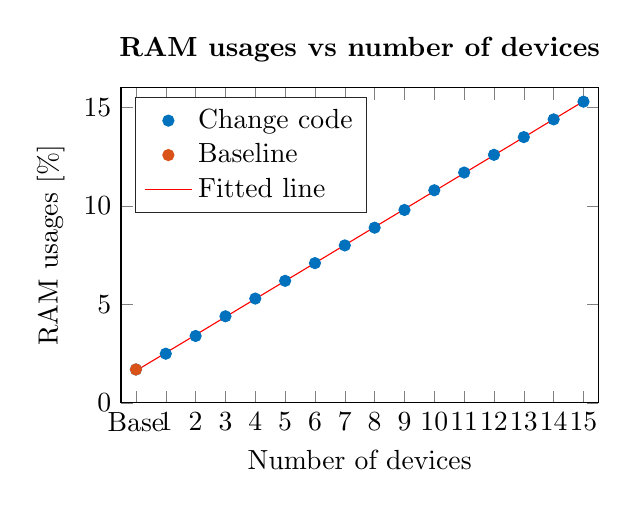
\begin{tikzpicture}

\begin{axis}[%
width=0.5\textwidth,
height=0.33\textwidth,
at={(0\textwidth,0\textwidth)},
scale only axis,
xmin=-0.5,
xmax=15.5,
xtick={0,1,2,3,4,5,6,7,8,9,10,11,12,13,14,15},
xticklabels={{Base},{1},{2},{3},{4},{5},{6},{7},{8},{9},{10},{11},{12},{13},{14},{15}},
xlabel={Number of devices},
ymin=0,
ymax=16,
ylabel={RAM usages [\%]},
axis background/.style={fill=white},
title style={font=\bfseries},
title={RAM usages vs number of devices},
legend style={at={(0.03,0.97)},anchor=north west,legend cell align=left,align=left,draw=white!15!black},
y tick label style={/pgf/number format/fixed}
]
\addplot [color=mycolor1,only marks,mark=*,mark options={solid}]
  table[row sep=crcr]{%
0	1.7\\
1	2.5\\
2	3.4\\
3	4.4\\
4	5.3\\
5	6.2\\
6	7.1\\
7	8\\
8	8.9\\
9	9.8\\
10	10.8\\
11	11.7\\
12	12.6\\
13	13.5\\
14	14.4\\
15	15.3\\
};
\addlegendentry{Change code};

\addplot [color=mycolor2,only marks,mark=*,mark options={solid}]
  table[row sep=crcr]{%
0	1.7\\
};
\addlegendentry{Baseline};

\addplot [color=red,solid]
  table[row sep=crcr]{%
0	1.63235294117647\\
0.015	1.64603823529412\\
0.03	1.65972352941176\\
0.045	1.67340882352941\\
0.06	1.68709411764706\\
0.075	1.70077941176471\\
0.09	1.71446470588235\\
0.105	1.72815\\
0.12	1.74183529411765\\
0.135	1.75552058823529\\
0.15	1.76920588235294\\
0.165	1.78289117647059\\
0.18	1.79657647058824\\
0.195	1.81026176470588\\
0.21	1.82394705882353\\
0.225	1.83763235294118\\
0.24	1.85131764705882\\
0.255	1.86500294117647\\
0.27	1.87868823529412\\
0.285	1.89237352941176\\
0.3	1.90605882352941\\
0.315	1.91974411764706\\
0.33	1.93342941176471\\
0.345	1.94711470588235\\
0.36	1.9608\\
0.375	1.97448529411765\\
0.39	1.98817058823529\\
0.405	2.00185588235294\\
0.42	2.01554117647059\\
0.435	2.02922647058824\\
0.45	2.04291176470588\\
0.465	2.05659705882353\\
0.48	2.07028235294118\\
0.495	2.08396764705882\\
0.51	2.09765294117647\\
0.525	2.11133823529412\\
0.54	2.12502352941176\\
0.555	2.13870882352941\\
0.57	2.15239411764706\\
0.585	2.16607941176471\\
0.6	2.17976470588235\\
0.615	2.19345\\
0.63	2.20713529411765\\
0.645	2.22082058823529\\
0.66	2.23450588235294\\
0.675	2.24819117647059\\
0.69	2.26187647058824\\
0.705	2.27556176470588\\
0.72	2.28924705882353\\
0.735	2.30293235294118\\
0.75	2.31661764705882\\
0.765	2.33030294117647\\
0.78	2.34398823529412\\
0.795	2.35767352941176\\
0.81	2.37135882352941\\
0.825	2.38504411764706\\
0.84	2.39872941176471\\
0.855	2.41241470588235\\
0.87	2.4261\\
0.885	2.43978529411765\\
0.9	2.45347058823529\\
0.915	2.46715588235294\\
0.93	2.48084117647059\\
0.945	2.49452647058824\\
0.96	2.50821176470588\\
0.975	2.52189705882353\\
0.99	2.53558235294118\\
1.005	2.54926764705882\\
1.02	2.56295294117647\\
1.035	2.57663823529412\\
1.05	2.59032352941176\\
1.065	2.60400882352941\\
1.08	2.61769411764706\\
1.095	2.63137941176471\\
1.11	2.64506470588235\\
1.125	2.65875\\
1.14	2.67243529411765\\
1.155	2.68612058823529\\
1.17	2.69980588235294\\
1.185	2.71349117647059\\
1.2	2.72717647058824\\
1.215	2.74086176470588\\
1.23	2.75454705882353\\
1.245	2.76823235294118\\
1.26	2.78191764705882\\
1.275	2.79560294117647\\
1.29	2.80928823529412\\
1.305	2.82297352941176\\
1.32	2.83665882352941\\
1.335	2.85034411764706\\
1.35	2.86402941176471\\
1.365	2.87771470588235\\
1.38	2.8914\\
1.395	2.90508529411765\\
1.41	2.91877058823529\\
1.425	2.93245588235294\\
1.44	2.94614117647059\\
1.455	2.95982647058824\\
1.47	2.97351176470588\\
1.485	2.98719705882353\\
1.5	3.00088235294118\\
1.515	3.01456764705882\\
1.53	3.02825294117647\\
1.545	3.04193823529412\\
1.56	3.05562352941176\\
1.575	3.06930882352941\\
1.59	3.08299411764706\\
1.605	3.09667941176471\\
1.62	3.11036470588235\\
1.635	3.12405\\
1.65	3.13773529411765\\
1.665	3.15142058823529\\
1.68	3.16510588235294\\
1.695	3.17879117647059\\
1.71	3.19247647058824\\
1.725	3.20616176470588\\
1.74	3.21984705882353\\
1.755	3.23353235294118\\
1.77	3.24721764705882\\
1.785	3.26090294117647\\
1.8	3.27458823529412\\
1.815	3.28827352941176\\
1.83	3.30195882352941\\
1.845	3.31564411764706\\
1.86	3.32932941176471\\
1.875	3.34301470588235\\
1.89	3.3567\\
1.905	3.37038529411765\\
1.92	3.38407058823529\\
1.935	3.39775588235294\\
1.95	3.41144117647059\\
1.965	3.42512647058824\\
1.98	3.43881176470588\\
1.995	3.45249705882353\\
2.01	3.46618235294118\\
2.025	3.47986764705882\\
2.04	3.49355294117647\\
2.055	3.50723823529412\\
2.07	3.52092352941176\\
2.085	3.53460882352941\\
2.1	3.54829411764706\\
2.115	3.56197941176471\\
2.13	3.57566470588235\\
2.145	3.58935\\
2.16	3.60303529411765\\
2.175	3.61672058823529\\
2.19	3.63040588235294\\
2.205	3.64409117647059\\
2.22	3.65777647058824\\
2.235	3.67146176470588\\
2.25	3.68514705882353\\
2.265	3.69883235294118\\
2.28	3.71251764705882\\
2.295	3.72620294117647\\
2.31	3.73988823529412\\
2.325	3.75357352941176\\
2.34	3.76725882352941\\
2.355	3.78094411764706\\
2.37	3.79462941176471\\
2.385	3.80831470588235\\
2.4	3.822\\
2.415	3.83568529411765\\
2.43	3.84937058823529\\
2.445	3.86305588235294\\
2.46	3.87674117647059\\
2.475	3.89042647058824\\
2.49	3.90411176470588\\
2.505	3.91779705882353\\
2.52	3.93148235294118\\
2.535	3.94516764705882\\
2.55	3.95885294117647\\
2.565	3.97253823529412\\
2.58	3.98622352941176\\
2.595	3.99990882352941\\
2.61	4.01359411764706\\
2.625	4.02727941176471\\
2.64	4.04096470588235\\
2.655	4.05465\\
2.67	4.06833529411765\\
2.685	4.08202058823529\\
2.7	4.09570588235294\\
2.715	4.10939117647059\\
2.73	4.12307647058824\\
2.745	4.13676176470588\\
2.76	4.15044705882353\\
2.775	4.16413235294118\\
2.79	4.17781764705882\\
2.805	4.19150294117647\\
2.82	4.20518823529412\\
2.835	4.21887352941176\\
2.85	4.23255882352941\\
2.865	4.24624411764706\\
2.88	4.25992941176471\\
2.895	4.27361470588235\\
2.91	4.2873\\
2.925	4.30098529411765\\
2.94	4.31467058823529\\
2.955	4.32835588235294\\
2.97	4.34204117647059\\
2.985	4.35572647058823\\
3	4.36941176470588\\
3.015	4.38309705882353\\
3.03	4.39678235294118\\
3.045	4.41046764705882\\
3.06	4.42415294117647\\
3.075	4.43783823529412\\
3.09	4.45152352941176\\
3.105	4.46520882352941\\
3.12	4.47889411764706\\
3.135	4.49257941176471\\
3.15	4.50626470588235\\
3.165	4.51995\\
3.18	4.53363529411765\\
3.195	4.54732058823529\\
3.21	4.56100588235294\\
3.225	4.57469117647059\\
3.24	4.58837647058824\\
3.255	4.60206176470588\\
3.27	4.61574705882353\\
3.285	4.62943235294118\\
3.3	4.64311764705882\\
3.315	4.65680294117647\\
3.33	4.67048823529412\\
3.345	4.68417352941176\\
3.36	4.69785882352941\\
3.375	4.71154411764706\\
3.39	4.72522941176471\\
3.405	4.73891470588235\\
3.42	4.7526\\
3.435	4.76628529411765\\
3.45	4.77997058823529\\
3.465	4.79365588235294\\
3.48	4.80734117647059\\
3.495	4.82102647058823\\
3.51	4.83471176470588\\
3.525	4.84839705882353\\
3.54	4.86208235294118\\
3.555	4.87576764705882\\
3.57	4.88945294117647\\
3.585	4.90313823529412\\
3.6	4.91682352941176\\
3.615	4.93050882352941\\
3.63	4.94419411764706\\
3.645	4.95787941176471\\
3.66	4.97156470588235\\
3.675	4.98525\\
3.69	4.99893529411765\\
3.705	5.01262058823529\\
3.72	5.02630588235294\\
3.735	5.03999117647059\\
3.75	5.05367647058824\\
3.765	5.06736176470588\\
3.78	5.08104705882353\\
3.795	5.09473235294118\\
3.81	5.10841764705882\\
3.825	5.12210294117647\\
3.84	5.13578823529412\\
3.855	5.14947352941176\\
3.87	5.16315882352941\\
3.885	5.17684411764706\\
3.9	5.19052941176471\\
3.915	5.20421470588235\\
3.93	5.2179\\
3.945	5.23158529411765\\
3.96	5.24527058823529\\
3.975	5.25895588235294\\
3.99	5.27264117647059\\
4.005	5.28632647058823\\
4.02	5.30001176470588\\
4.035	5.31369705882353\\
4.05	5.32738235294118\\
4.065	5.34106764705882\\
4.08	5.35475294117647\\
4.095	5.36843823529412\\
4.11	5.38212352941176\\
4.125	5.39580882352941\\
4.14	5.40949411764706\\
4.155	5.42317941176471\\
4.17	5.43686470588235\\
4.185	5.45055\\
4.2	5.46423529411765\\
4.215	5.47792058823529\\
4.23	5.49160588235294\\
4.245	5.50529117647059\\
4.26	5.51897647058823\\
4.275	5.53266176470588\\
4.29	5.54634705882353\\
4.305	5.56003235294118\\
4.32	5.57371764705882\\
4.335	5.58740294117647\\
4.35	5.60108823529412\\
4.365	5.61477352941176\\
4.38	5.62845882352941\\
4.395	5.64214411764706\\
4.41	5.65582941176471\\
4.425	5.66951470588235\\
4.44	5.6832\\
4.455	5.69688529411765\\
4.47	5.71057058823529\\
4.485	5.72425588235294\\
4.5	5.73794117647059\\
4.515	5.75162647058824\\
4.53	5.76531176470588\\
4.545	5.77899705882353\\
4.56	5.79268235294118\\
4.575	5.80636764705882\\
4.59	5.82005294117647\\
4.605	5.83373823529412\\
4.62	5.84742352941177\\
4.635	5.86110882352941\\
4.65	5.87479411764706\\
4.665	5.88847941176471\\
4.68	5.90216470588235\\
4.695	5.91585\\
4.71	5.92953529411765\\
4.725	5.94322058823529\\
4.74	5.95690588235294\\
4.755	5.97059117647059\\
4.77	5.98427647058823\\
4.785	5.99796176470588\\
4.8	6.01164705882353\\
4.815	6.02533235294118\\
4.83	6.03901764705882\\
4.845	6.05270294117647\\
4.86	6.06638823529412\\
4.875	6.08007352941176\\
4.89	6.09375882352941\\
4.905	6.10744411764706\\
4.92	6.12112941176471\\
4.935	6.13481470588235\\
4.95	6.1485\\
4.965	6.16218529411765\\
4.98	6.17587058823529\\
4.995	6.18955588235294\\
5.01	6.20324117647059\\
5.025	6.21692647058824\\
5.04	6.23061176470588\\
5.055	6.24429705882353\\
5.07	6.25798235294118\\
5.085	6.27166764705882\\
5.1	6.28535294117647\\
5.115	6.29903823529412\\
5.13	6.31272352941176\\
5.145	6.32640882352941\\
5.16	6.34009411764706\\
5.175	6.35377941176471\\
5.19	6.36746470588235\\
5.205	6.38115\\
5.22	6.39483529411765\\
5.235	6.40852058823529\\
5.25	6.42220588235294\\
5.265	6.43589117647059\\
5.28	6.44957647058823\\
5.295	6.46326176470588\\
5.31	6.47694705882353\\
5.325	6.49063235294118\\
5.34	6.50431764705882\\
5.355	6.51800294117647\\
5.37	6.53168823529412\\
5.385	6.54537352941176\\
5.4	6.55905882352941\\
5.415	6.57274411764706\\
5.43	6.58642941176471\\
5.445	6.60011470588235\\
5.46	6.6138\\
5.475	6.62748529411765\\
5.49	6.64117058823529\\
5.505	6.65485588235294\\
5.52	6.66854117647059\\
5.535	6.68222647058824\\
5.55	6.69591176470588\\
5.565	6.70959705882353\\
5.58	6.72328235294118\\
5.595	6.73696764705882\\
5.61	6.75065294117647\\
5.625	6.76433823529412\\
5.64	6.77802352941176\\
5.655	6.79170882352941\\
5.67	6.80539411764706\\
5.685	6.81907941176471\\
5.7	6.83276470588235\\
5.715	6.84645\\
5.73	6.86013529411765\\
5.745	6.87382058823529\\
5.76	6.88750588235294\\
5.775	6.90119117647059\\
5.79	6.91487647058824\\
5.805	6.92856176470588\\
5.82	6.94224705882353\\
5.835	6.95593235294118\\
5.85	6.96961764705882\\
5.865	6.98330294117647\\
5.88	6.99698823529412\\
5.895	7.01067352941176\\
5.91	7.02435882352941\\
5.925	7.03804411764706\\
5.94	7.0517294117647\\
5.955	7.06541470588235\\
5.97	7.0791\\
5.985	7.09278529411765\\
6	7.10647058823529\\
6.015	7.12015588235294\\
6.03	7.13384117647059\\
6.045	7.14752647058824\\
6.06	7.16121176470588\\
6.075	7.17489705882353\\
6.09	7.18858235294118\\
6.105	7.20226764705882\\
6.12	7.21595294117647\\
6.135	7.22963823529412\\
6.15	7.24332352941176\\
6.165	7.25700882352941\\
6.18	7.27069411764706\\
6.195	7.28437941176471\\
6.21	7.29806470588235\\
6.225	7.31175\\
6.24	7.32543529411765\\
6.255	7.33912058823529\\
6.27	7.35280588235294\\
6.285	7.36649117647059\\
6.3	7.38017647058823\\
6.315	7.39386176470588\\
6.33	7.40754705882353\\
6.345	7.42123235294118\\
6.36	7.43491764705882\\
6.375	7.44860294117647\\
6.39	7.46228823529412\\
6.405	7.47597352941176\\
6.42	7.48965882352941\\
6.435	7.50334411764706\\
6.45	7.51702941176471\\
6.465	7.53071470588235\\
6.48	7.5444\\
6.495	7.55808529411765\\
6.51	7.57177058823529\\
6.525	7.58545588235294\\
6.54	7.59914117647059\\
6.555	7.61282647058824\\
6.57	7.62651176470588\\
6.585	7.64019705882353\\
6.6	7.65388235294118\\
6.615	7.66756764705882\\
6.63	7.68125294117647\\
6.645	7.69493823529412\\
6.66	7.70862352941176\\
6.675	7.72230882352941\\
6.69	7.73599411764706\\
6.705	7.74967941176471\\
6.72	7.76336470588235\\
6.735	7.77705\\
6.75	7.79073529411765\\
6.765	7.80442058823529\\
6.78	7.81810588235294\\
6.795	7.83179117647059\\
6.81	7.84547647058823\\
6.825	7.85916176470588\\
6.84	7.87284705882353\\
6.855	7.88653235294118\\
6.87	7.90021764705882\\
6.885	7.91390294117647\\
6.9	7.92758823529412\\
6.915	7.94127352941176\\
6.93	7.95495882352941\\
6.945	7.96864411764706\\
6.96	7.98232941176471\\
6.975	7.99601470588235\\
6.99	8.0097\\
7.005	8.02338529411765\\
7.02	8.03707058823529\\
7.035	8.05075588235294\\
7.05	8.06444117647059\\
7.065	8.07812647058823\\
7.08	8.09181176470588\\
7.095	8.10549705882353\\
7.11	8.11918235294118\\
7.125	8.13286764705882\\
7.14	8.14655294117647\\
7.155	8.16023823529412\\
7.17	8.17392352941176\\
7.185	8.18760882352941\\
7.2	8.20129411764706\\
7.215	8.21497941176471\\
7.23	8.22866470588235\\
7.245	8.24235\\
7.26	8.25603529411765\\
7.275	8.26972058823529\\
7.29	8.28340588235294\\
7.305	8.29709117647059\\
7.32	8.31077647058823\\
7.335	8.32446176470588\\
7.35	8.33814705882353\\
7.365	8.35183235294117\\
7.38	8.36551764705882\\
7.395	8.37920294117647\\
7.41	8.39288823529412\\
7.425	8.40657352941176\\
7.44	8.42025882352941\\
7.455	8.43394411764706\\
7.47	8.44762941176471\\
7.485	8.46131470588235\\
7.5	8.475\\
7.515	8.48868529411765\\
7.53	8.50237058823529\\
7.545	8.51605588235294\\
7.56	8.52974117647059\\
7.575	8.54342647058823\\
7.59	8.55711176470588\\
7.605	8.57079705882353\\
7.62	8.58448235294118\\
7.635	8.59816764705882\\
7.65	8.61185294117647\\
7.665	8.62553823529412\\
7.68	8.63922352941176\\
7.695	8.65290882352941\\
7.71	8.66659411764706\\
7.725	8.6802794117647\\
7.74	8.69396470588235\\
7.755	8.70765\\
7.77	8.72133529411765\\
7.785	8.73502058823529\\
7.8	8.74870588235294\\
7.815	8.76239117647059\\
7.83	8.77607647058823\\
7.845	8.78976176470588\\
7.86	8.80344705882353\\
7.875	8.81713235294118\\
7.89	8.83081764705882\\
7.905	8.84450294117647\\
7.92	8.85818823529412\\
7.935	8.87187352941176\\
7.95	8.88555882352941\\
7.965	8.89924411764706\\
7.98	8.9129294117647\\
7.995	8.92661470588235\\
8.01	8.9403\\
8.025	8.95398529411765\\
8.04	8.96767058823529\\
8.055	8.98135588235294\\
8.07	8.99504117647059\\
8.085	9.00872647058823\\
8.1	9.02241176470588\\
8.115	9.03609705882353\\
8.13	9.04978235294118\\
8.145	9.06346764705882\\
8.16	9.07715294117647\\
8.175	9.09083823529412\\
8.19	9.10452352941176\\
8.205	9.11820882352941\\
8.22	9.13189411764706\\
8.235	9.1455794117647\\
8.25	9.15926470588235\\
8.265	9.17295\\
8.28	9.18663529411764\\
8.295	9.20032058823529\\
8.31	9.21400588235294\\
8.325	9.22769117647059\\
8.34	9.24137647058823\\
8.355	9.25506176470588\\
8.37	9.26874705882353\\
8.385	9.28243235294118\\
8.4	9.29611764705882\\
8.415	9.30980294117647\\
8.43	9.32348823529412\\
8.445	9.33717352941176\\
8.46	9.35085882352941\\
8.475	9.36454411764706\\
8.49	9.37822941176471\\
8.505	9.39191470588235\\
8.52	9.4056\\
8.535	9.41928529411765\\
8.55	9.43297058823529\\
8.565	9.44665588235294\\
8.58	9.46034117647059\\
8.595	9.47402647058823\\
8.61	9.48771176470588\\
8.625	9.50139705882353\\
8.64	9.51508235294118\\
8.655	9.52876764705882\\
8.67	9.54245294117647\\
8.685	9.55613823529412\\
8.7	9.56982352941176\\
8.715	9.58350882352941\\
8.73	9.59719411764706\\
8.745	9.6108794117647\\
8.76	9.62456470588235\\
8.775	9.63825\\
8.79	9.65193529411765\\
8.805	9.66562058823529\\
8.82	9.67930588235294\\
8.835	9.69299117647059\\
8.85	9.70667647058823\\
8.865	9.72036176470588\\
8.88	9.73404705882353\\
8.895	9.74773235294118\\
8.91	9.76141764705882\\
8.925	9.77510294117647\\
8.94	9.78878823529412\\
8.955	9.80247352941177\\
8.97	9.81615882352941\\
8.985	9.82984411764706\\
9	9.84352941176471\\
9.015	9.85721470588235\\
9.03	9.8709\\
9.045	9.88458529411765\\
9.06	9.89827058823529\\
9.075	9.91195588235294\\
9.09	9.92564117647059\\
9.105	9.93932647058823\\
9.12	9.95301176470588\\
9.135	9.96669705882353\\
9.15	9.98038235294118\\
9.165	9.99406764705882\\
9.18	10.0077529411765\\
9.195	10.0214382352941\\
9.21	10.0351235294118\\
9.225	10.0488088235294\\
9.24	10.0624941176471\\
9.255	10.0761794117647\\
9.27	10.0898647058824\\
9.285	10.10355\\
9.3	10.1172352941176\\
9.315	10.1309205882353\\
9.33	10.1446058823529\\
9.345	10.1582911764706\\
9.36	10.1719764705882\\
9.375	10.1856617647059\\
9.39	10.1993470588235\\
9.405	10.2130323529412\\
9.42	10.2267176470588\\
9.435	10.2404029411765\\
9.45	10.2540882352941\\
9.465	10.2677735294118\\
9.48	10.2814588235294\\
9.495	10.2951441176471\\
9.51	10.3088294117647\\
9.525	10.3225147058824\\
9.54	10.3362\\
9.555	10.3498852941176\\
9.57	10.3635705882353\\
9.585	10.3772558823529\\
9.6	10.3909411764706\\
9.615	10.4046264705882\\
9.63	10.4183117647059\\
9.645	10.4319970588235\\
9.66	10.4456823529412\\
9.675	10.4593676470588\\
9.69	10.4730529411765\\
9.705	10.4867382352941\\
9.72	10.5004235294118\\
9.735	10.5141088235294\\
9.75	10.5277941176471\\
9.765	10.5414794117647\\
9.78	10.5551647058824\\
9.795	10.56885\\
9.81	10.5825352941176\\
9.825	10.5962205882353\\
9.84	10.6099058823529\\
9.855	10.6235911764706\\
9.87	10.6372764705882\\
9.885	10.6509617647059\\
9.9	10.6646470588235\\
9.915	10.6783323529412\\
9.93	10.6920176470588\\
9.945	10.7057029411765\\
9.96	10.7193882352941\\
9.975	10.7330735294118\\
9.99	10.7467588235294\\
10.005	10.7604441176471\\
10.02	10.7741294117647\\
10.035	10.7878147058824\\
10.05	10.8015\\
10.065	10.8151852941176\\
10.08	10.8288705882353\\
10.095	10.8425558823529\\
10.11	10.8562411764706\\
10.125	10.8699264705882\\
10.14	10.8836117647059\\
10.155	10.8972970588235\\
10.17	10.9109823529412\\
10.185	10.9246676470588\\
10.2	10.9383529411765\\
10.215	10.9520382352941\\
10.23	10.9657235294118\\
10.245	10.9794088235294\\
10.26	10.9930941176471\\
10.275	11.0067794117647\\
10.29	11.0204647058824\\
10.305	11.03415\\
10.32	11.0478352941176\\
10.335	11.0615205882353\\
10.35	11.0752058823529\\
10.365	11.0888911764706\\
10.38	11.1025764705882\\
10.395	11.1162617647059\\
10.41	11.1299470588235\\
10.425	11.1436323529412\\
10.44	11.1573176470588\\
10.455	11.1710029411765\\
10.47	11.1846882352941\\
10.485	11.1983735294118\\
10.5	11.2120588235294\\
10.515	11.2257441176471\\
10.53	11.2394294117647\\
10.545	11.2531147058824\\
10.56	11.2668\\
10.575	11.2804852941176\\
10.59	11.2941705882353\\
10.605	11.3078558823529\\
10.62	11.3215411764706\\
10.635	11.3352264705882\\
10.65	11.3489117647059\\
10.665	11.3625970588235\\
10.68	11.3762823529412\\
10.695	11.3899676470588\\
10.71	11.4036529411765\\
10.725	11.4173382352941\\
10.74	11.4310235294118\\
10.755	11.4447088235294\\
10.77	11.4583941176471\\
10.785	11.4720794117647\\
10.8	11.4857647058824\\
10.815	11.49945\\
10.83	11.5131352941176\\
10.845	11.5268205882353\\
10.86	11.5405058823529\\
10.875	11.5541911764706\\
10.89	11.5678764705882\\
10.905	11.5815617647059\\
10.92	11.5952470588235\\
10.935	11.6089323529412\\
10.95	11.6226176470588\\
10.965	11.6363029411765\\
10.98	11.6499882352941\\
10.995	11.6636735294118\\
11.01	11.6773588235294\\
11.025	11.6910441176471\\
11.04	11.7047294117647\\
11.055	11.7184147058824\\
11.07	11.7321\\
11.085	11.7457852941176\\
11.1	11.7594705882353\\
11.115	11.7731558823529\\
11.13	11.7868411764706\\
11.145	11.8005264705882\\
11.16	11.8142117647059\\
11.175	11.8278970588235\\
11.19	11.8415823529412\\
11.205	11.8552676470588\\
11.22	11.8689529411765\\
11.235	11.8826382352941\\
11.25	11.8963235294118\\
11.265	11.9100088235294\\
11.28	11.9236941176471\\
11.295	11.9373794117647\\
11.31	11.9510647058824\\
11.325	11.96475\\
11.34	11.9784352941176\\
11.355	11.9921205882353\\
11.37	12.0058058823529\\
11.385	12.0194911764706\\
11.4	12.0331764705882\\
11.415	12.0468617647059\\
11.43	12.0605470588235\\
11.445	12.0742323529412\\
11.46	12.0879176470588\\
11.475	12.1016029411765\\
11.49	12.1152882352941\\
11.505	12.1289735294118\\
11.52	12.1426588235294\\
11.535	12.1563441176471\\
11.55	12.1700294117647\\
11.565	12.1837147058824\\
11.58	12.1974\\
11.595	12.2110852941176\\
11.61	12.2247705882353\\
11.625	12.2384558823529\\
11.64	12.2521411764706\\
11.655	12.2658264705882\\
11.67	12.2795117647059\\
11.685	12.2931970588235\\
11.7	12.3068823529412\\
11.715	12.3205676470588\\
11.73	12.3342529411765\\
11.745	12.3479382352941\\
11.76	12.3616235294118\\
11.775	12.3753088235294\\
11.79	12.3889941176471\\
11.805	12.4026794117647\\
11.82	12.4163647058824\\
11.835	12.43005\\
11.85	12.4437352941176\\
11.865	12.4574205882353\\
11.88	12.4711058823529\\
11.895	12.4847911764706\\
11.91	12.4984764705882\\
11.925	12.5121617647059\\
11.94	12.5258470588235\\
11.955	12.5395323529412\\
11.97	12.5532176470588\\
11.985	12.5669029411765\\
12	12.5805882352941\\
12.015	12.5942735294118\\
12.03	12.6079588235294\\
12.045	12.6216441176471\\
12.06	12.6353294117647\\
12.075	12.6490147058824\\
12.09	12.6627\\
12.105	12.6763852941176\\
12.12	12.6900705882353\\
12.135	12.7037558823529\\
12.15	12.7174411764706\\
12.165	12.7311264705882\\
12.18	12.7448117647059\\
12.195	12.7584970588235\\
12.21	12.7721823529412\\
12.225	12.7858676470588\\
12.24	12.7995529411765\\
12.255	12.8132382352941\\
12.27	12.8269235294118\\
12.285	12.8406088235294\\
12.3	12.8542941176471\\
12.315	12.8679794117647\\
12.33	12.8816647058824\\
12.345	12.89535\\
12.36	12.9090352941176\\
12.375	12.9227205882353\\
12.39	12.9364058823529\\
12.405	12.9500911764706\\
12.42	12.9637764705882\\
12.435	12.9774617647059\\
12.45	12.9911470588235\\
12.465	13.0048323529412\\
12.48	13.0185176470588\\
12.495	13.0322029411765\\
12.51	13.0458882352941\\
12.525	13.0595735294118\\
12.54	13.0732588235294\\
12.555	13.0869441176471\\
12.57	13.1006294117647\\
12.585	13.1143147058824\\
12.6	13.128\\
12.615	13.1416852941176\\
12.63	13.1553705882353\\
12.645	13.1690558823529\\
12.66	13.1827411764706\\
12.675	13.1964264705882\\
12.69	13.2101117647059\\
12.705	13.2237970588235\\
12.72	13.2374823529412\\
12.735	13.2511676470588\\
12.75	13.2648529411765\\
12.765	13.2785382352941\\
12.78	13.2922235294118\\
12.795	13.3059088235294\\
12.81	13.3195941176471\\
12.825	13.3332794117647\\
12.84	13.3469647058824\\
12.855	13.36065\\
12.87	13.3743352941176\\
12.885	13.3880205882353\\
12.9	13.4017058823529\\
12.915	13.4153911764706\\
12.93	13.4290764705882\\
12.945	13.4427617647059\\
12.96	13.4564470588235\\
12.975	13.4701323529412\\
12.99	13.4838176470588\\
13.005	13.4975029411765\\
13.02	13.5111882352941\\
13.035	13.5248735294118\\
13.05	13.5385588235294\\
13.065	13.5522441176471\\
13.08	13.5659294117647\\
13.095	13.5796147058824\\
13.11	13.5933\\
13.125	13.6069852941176\\
13.14	13.6206705882353\\
13.155	13.6343558823529\\
13.17	13.6480411764706\\
13.185	13.6617264705882\\
13.2	13.6754117647059\\
13.215	13.6890970588235\\
13.23	13.7027823529412\\
13.245	13.7164676470588\\
13.26	13.7301529411765\\
13.275	13.7438382352941\\
13.29	13.7575235294118\\
13.305	13.7712088235294\\
13.32	13.7848941176471\\
13.335	13.7985794117647\\
13.35	13.8122647058824\\
13.365	13.82595\\
13.38	13.8396352941176\\
13.395	13.8533205882353\\
13.41	13.8670058823529\\
13.425	13.8806911764706\\
13.44	13.8943764705882\\
13.455	13.9080617647059\\
13.47	13.9217470588235\\
13.485	13.9354323529412\\
13.5	13.9491176470588\\
13.515	13.9628029411765\\
13.53	13.9764882352941\\
13.545	13.9901735294118\\
13.56	14.0038588235294\\
13.575	14.0175441176471\\
13.59	14.0312294117647\\
13.605	14.0449147058824\\
13.62	14.0586\\
13.635	14.0722852941176\\
13.65	14.0859705882353\\
13.665	14.0996558823529\\
13.68	14.1133411764706\\
13.695	14.1270264705882\\
13.71	14.1407117647059\\
13.725	14.1543970588235\\
13.74	14.1680823529412\\
13.755	14.1817676470588\\
13.77	14.1954529411765\\
13.785	14.2091382352941\\
13.8	14.2228235294118\\
13.815	14.2365088235294\\
13.83	14.2501941176471\\
13.845	14.2638794117647\\
13.86	14.2775647058824\\
13.875	14.29125\\
13.89	14.3049352941176\\
13.905	14.3186205882353\\
13.92	14.3323058823529\\
13.935	14.3459911764706\\
13.95	14.3596764705882\\
13.965	14.3733617647059\\
13.98	14.3870470588235\\
13.995	14.4007323529412\\
14.01	14.4144176470588\\
14.025	14.4281029411765\\
14.04	14.4417882352941\\
14.055	14.4554735294118\\
14.07	14.4691588235294\\
14.085	14.4828441176471\\
14.1	14.4965294117647\\
14.115	14.5102147058824\\
14.13	14.5239\\
14.145	14.5375852941176\\
14.16	14.5512705882353\\
14.175	14.5649558823529\\
14.19	14.5786411764706\\
14.205	14.5923264705882\\
14.22	14.6060117647059\\
14.235	14.6196970588235\\
14.25	14.6333823529412\\
14.265	14.6470676470588\\
14.28	14.6607529411765\\
14.295	14.6744382352941\\
14.31	14.6881235294118\\
14.325	14.7018088235294\\
14.34	14.7154941176471\\
14.355	14.7291794117647\\
14.37	14.7428647058824\\
14.385	14.75655\\
14.4	14.7702352941176\\
14.415	14.7839205882353\\
14.43	14.7976058823529\\
14.445	14.8112911764706\\
14.46	14.8249764705882\\
14.475	14.8386617647059\\
14.49	14.8523470588235\\
14.505	14.8660323529412\\
14.52	14.8797176470588\\
14.535	14.8934029411765\\
14.55	14.9070882352941\\
14.565	14.9207735294118\\
14.58	14.9344588235294\\
14.595	14.9481441176471\\
14.61	14.9618294117647\\
14.625	14.9755147058824\\
14.64	14.9892\\
14.655	15.0028852941176\\
14.67	15.0165705882353\\
14.685	15.0302558823529\\
14.7	15.0439411764706\\
14.715	15.0576264705882\\
14.73	15.0713117647059\\
14.745	15.0849970588235\\
14.76	15.0986823529412\\
14.775	15.1123676470588\\
14.79	15.1260529411765\\
14.805	15.1397382352941\\
14.82	15.1534235294118\\
14.835	15.1671088235294\\
14.85	15.1807941176471\\
14.865	15.1944794117647\\
14.88	15.2081647058824\\
14.895	15.22185\\
14.91	15.2355352941176\\
14.925	15.2492205882353\\
14.94	15.2629058823529\\
14.955	15.2765911764706\\
14.97	15.2902764705882\\
14.985	15.3039617647059\\
15	15.3176470588235\\
};
\addlegendentry{Fitted line};

\end{axis}
\end{tikzpicture}%}
\caption{Memory usage for the whole process for different number of devices in the MDE and the baseline emulator. The fitted line is a linear approximation}
\label{fig:RAMusage}
\end{figure}

The fitted line for the CPU usage is estimated to be:
\begin{equation}
RAM = 0.91 \cdot NoD + 1.63
\end{equation}


As seen in \autoref{fig:RAMusage}, the memory usage follow a very linear tendency. This makes sense, as the whole structure is multiplied with the number of device and therefore also the memory usage. The reason for the difference between the baseline emulator and a single device, is the that the Co Phy use as much space as a normal device, as describe in \autoref{sec:Changes}. With the computer used for the project, the limit for number of devices that can emulated, when only looking at the memory usage, is 108 devices.



